\documentclass[twoside]{book}

% Packages required by doxygen
\usepackage{fixltx2e}
\usepackage{calc}
\usepackage{doxygen}
\usepackage[export]{adjustbox} % also loads graphicx
\usepackage{graphicx}
\usepackage[utf8]{inputenc}
\usepackage{makeidx}
\usepackage{multicol}
\usepackage{multirow}
\PassOptionsToPackage{warn}{textcomp}
\usepackage{textcomp}
\usepackage[nointegrals]{wasysym}
\usepackage[table]{xcolor}

% Font selection
\usepackage[T1]{fontenc}
\usepackage[scaled=.90]{helvet}
\usepackage{courier}
\usepackage{amssymb}
\usepackage{sectsty}
\renewcommand{\familydefault}{\sfdefault}
\allsectionsfont{%
  \fontseries{bc}\selectfont%
  \color{darkgray}%
}
\renewcommand{\DoxyLabelFont}{%
  \fontseries{bc}\selectfont%
  \color{darkgray}%
}
\newcommand{\+}{\discretionary{\mbox{\scriptsize$\hookleftarrow$}}{}{}}

% Page & text layout
\usepackage{geometry}
\geometry{%
  a4paper,%
  top=2.5cm,%
  bottom=2.5cm,%
  left=2.5cm,%
  right=2.5cm%
}
\tolerance=750
\hfuzz=15pt
\hbadness=750
\setlength{\emergencystretch}{15pt}
\setlength{\parindent}{0cm}
\setlength{\parskip}{3ex plus 2ex minus 2ex}
\makeatletter
\renewcommand{\paragraph}{%
  \@startsection{paragraph}{4}{0ex}{-1.0ex}{1.0ex}{%
    \normalfont\normalsize\bfseries\SS@parafont%
  }%
}
\renewcommand{\subparagraph}{%
  \@startsection{subparagraph}{5}{0ex}{-1.0ex}{1.0ex}{%
    \normalfont\normalsize\bfseries\SS@subparafont%
  }%
}
\makeatother

% Headers & footers
\usepackage{fancyhdr}
\pagestyle{fancyplain}
\fancyhead[LE]{\fancyplain{}{\bfseries\thepage}}
\fancyhead[CE]{\fancyplain{}{}}
\fancyhead[RE]{\fancyplain{}{\bfseries\leftmark}}
\fancyhead[LO]{\fancyplain{}{\bfseries\rightmark}}
\fancyhead[CO]{\fancyplain{}{}}
\fancyhead[RO]{\fancyplain{}{\bfseries\thepage}}
\fancyfoot[LE]{\fancyplain{}{}}
\fancyfoot[CE]{\fancyplain{}{}}
\fancyfoot[RE]{\fancyplain{}{\bfseries\scriptsize Generated by Doxygen }}
\fancyfoot[LO]{\fancyplain{}{\bfseries\scriptsize Generated by Doxygen }}
\fancyfoot[CO]{\fancyplain{}{}}
\fancyfoot[RO]{\fancyplain{}{}}
\renewcommand{\footrulewidth}{0.4pt}
\renewcommand{\chaptermark}[1]{%
  \markboth{#1}{}%
}
\renewcommand{\sectionmark}[1]{%
  \markright{\thesection\ #1}%
}

% Indices & bibliography
\usepackage{natbib}
\usepackage[titles]{tocloft}
\setcounter{tocdepth}{3}
\setcounter{secnumdepth}{5}
\makeindex

% Hyperlinks (required, but should be loaded last)
\usepackage{ifpdf}
\ifpdf
  \usepackage[pdftex,pagebackref=true]{hyperref}
\else
  \usepackage[ps2pdf,pagebackref=true]{hyperref}
\fi
\hypersetup{%
  colorlinks=true,%
  linkcolor=blue,%
  citecolor=blue,%
  unicode%
}

% Custom commands
\newcommand{\clearemptydoublepage}{%
  \newpage{\pagestyle{empty}\cleardoublepage}%
}

\usepackage{caption}
\captionsetup{labelsep=space,justification=centering,font={bf},singlelinecheck=off,skip=4pt,position=top}

%===== C O N T E N T S =====

\begin{document}

% Titlepage & ToC
\hypersetup{pageanchor=false,
             bookmarksnumbered=true,
             pdfencoding=unicode
            }
\pagenumbering{alph}
\begin{titlepage}
\vspace*{7cm}
\begin{center}%
{\Large E\+T\+VO \\[1ex]\large 2.\+0 }\\
\vspace*{1cm}
{\large Generated by Doxygen 1.8.14}\\
\end{center}
\end{titlepage}
\clearemptydoublepage
\pagenumbering{roman}
\tableofcontents
\clearemptydoublepage
\pagenumbering{arabic}
\hypersetup{pageanchor=true}

%--- Begin generated contents ---
\chapter{\mbox{[}E\+T\+VO (Event$\vert$\+Time-\/\+Variant Operators)\mbox{]}}
\label{index}\hypertarget{index}{}

\begin{DoxyAuthor}{Authors}
B.\+Cottenceau L.\+Hardouin J.\+Trunk (Laboratory L\+A\+R\+IS -\/ Angers -\/ F\+R\+A\+N\+CE)
\end{DoxyAuthor}
\section{Introduction}\label{index_Introduction}
This library is a set of classes to make computations on formal series used in Discrete Event Systems. More specifically, these series allow us to describe the behaviour of a subclass of Petri Nets The formal series handled with this library lie on a set of elementary operators used to describe Timed Event Graphs (T\+E\+Gs), Weighted Timed Event Graphs (W\+T\+E\+Gs) and some Timed Event Graphs with time-\/variant sojourn times. 
\chapter{Namespace Index}
\section{Namespace List}
Here is a list of all documented namespaces with brief descriptions\+:\begin{DoxyCompactList}
\item\contentsline{section}{\mbox{\hyperlink{namespaceetvo_i_i}{etvo\+II}} }{\pageref{namespaceetvo_i_i}}{}
\end{DoxyCompactList}

\chapter{Hierarchical Index}
\section{Class Hierarchy}
This inheritance list is sorted roughly, but not completely, alphabetically\+:\begin{DoxyCompactList}
\item \contentsline{section}{Pov\+Ray\+:\+:Pov\+Ray2\+:\+:Color}{\pageref{class_pov_ray_1_1_pov_ray2_1_1_color}}{}
\item \contentsline{section}{etvo\+II\+:\+:d\+Dd}{\pageref{classetvo_i_i_1_1d_dd}}{}
\item \contentsline{section}{etvo\+II\+:\+:E\+\_\+op}{\pageref{classetvo_i_i_1_1_e__op}}{}
\item \contentsline{section}{etvo\+II\+:\+:Ed}{\pageref{classetvo_i_i_1_1_ed}}{}
\item exception\begin{DoxyCompactList}
\item \contentsline{section}{etvo\+II\+:\+:etvo\+Exception}{\pageref{classetvo_i_i_1_1etvo_exception}}{}
\item \contentsline{section}{test\+:\+:test\+Exception}{\pageref{classtest_1_1test_exception}}{}
\end{DoxyCompactList}
\item \contentsline{section}{etvo\+II\+:\+:Factory$<$ T $>$}{\pageref{classetvo_i_i_1_1_factory}}{}
\item \contentsline{section}{etvo\+II\+:\+:Factory$<$ etvo\+II\+:\+:poly $>$}{\pageref{classetvo_i_i_1_1_factory}}{}
\begin{DoxyCompactList}
\item \contentsline{section}{etvo\+II\+:\+:Factory\+Poly}{\pageref{classetvo_i_i_1_1_factory_poly}}{}
\end{DoxyCompactList}
\item \contentsline{section}{etvo\+II\+:\+:Factory$<$ etvo\+II\+:\+:series $>$}{\pageref{classetvo_i_i_1_1_factory}}{}
\begin{DoxyCompactList}
\item \contentsline{section}{etvo\+II\+:\+:Factory\+Series}{\pageref{classetvo_i_i_1_1_factory_series}}{}
\end{DoxyCompactList}
\item \contentsline{section}{etvo\+II\+:\+:Factory$<$ Fper $>$}{\pageref{classetvo_i_i_1_1_factory}}{}
\begin{DoxyCompactList}
\item \contentsline{section}{etvo\+II\+:\+:Factory\+Fper}{\pageref{classetvo_i_i_1_1_factory_fper}}{}
\end{DoxyCompactList}
\item \contentsline{section}{etvo\+II\+:\+:Factory$<$ poly\+Ed $>$}{\pageref{classetvo_i_i_1_1_factory}}{}
\begin{DoxyCompactList}
\item \contentsline{section}{etvo\+II\+:\+:Factory\+Poly\+Ed}{\pageref{classetvo_i_i_1_1_factory_poly_ed}}{}
\end{DoxyCompactList}
\item \contentsline{section}{etvo\+II\+:\+:Factory$<$ poly\+Tg $>$}{\pageref{classetvo_i_i_1_1_factory}}{}
\begin{DoxyCompactList}
\item \contentsline{section}{etvo\+II\+:\+:Factory\+Poly\+Tg}{\pageref{classetvo_i_i_1_1_factory_poly_tg}}{}
\end{DoxyCompactList}
\item \contentsline{section}{etvo\+II\+:\+:Factory$<$ series\+Ed $>$}{\pageref{classetvo_i_i_1_1_factory}}{}
\begin{DoxyCompactList}
\item \contentsline{section}{etvo\+II\+:\+:Factory\+Series\+Ed}{\pageref{classetvo_i_i_1_1_factory_series_ed}}{}
\end{DoxyCompactList}
\item \contentsline{section}{etvo\+II\+:\+:Fper}{\pageref{classetvo_i_i_1_1_fper}}{}
\begin{DoxyCompactList}
\item \contentsline{section}{etvo\+II\+:\+:Fmaxp}{\pageref{classetvo_i_i_1_1_fmaxp}}{}
\item \contentsline{section}{etvo\+II\+:\+:Fminp}{\pageref{classetvo_i_i_1_1_fminp}}{}
\end{DoxyCompactList}
\item \contentsline{section}{mmgd\+:\+:gd}{\pageref{classmmgd_1_1gd}}{}
\begin{DoxyCompactList}
\item \contentsline{section}{etvo\+II\+:\+:gd}{\pageref{classetvo_i_i_1_1gd}}{}
\end{DoxyCompactList}
\item \contentsline{section}{global}{\pageref{classglobal}}{}
\item \contentsline{section}{etvo\+II\+:\+:g\+Ng}{\pageref{classetvo_i_i_1_1g_ng}}{}
\item grammar\begin{DoxyCompactList}
\item \contentsline{section}{calculator\+Etvo\+:\+:calculator$<$ Iterator $>$}{\pageref{structcalculator_etvo_1_1calculator}}{}
\item \contentsline{section}{parseped\+:\+:calculator$<$ Iterator $>$}{\pageref{structparseped_1_1calculator}}{}
\item \contentsline{section}{parsepoly\+I\+II\+:\+:calculator$<$ Iterator $>$}{\pageref{structparsepoly_i_i_i_1_1calculator}}{}
\item \contentsline{section}{parseptg\+:\+:calculator$<$ Iterator $>$}{\pageref{structparseptg_1_1calculator}}{}
\item \contentsline{section}{parseseriesed\+:\+:calculator$<$ Iterator $>$}{\pageref{structparseseriesed_1_1calculator}}{}
\end{DoxyCompactList}
\item \contentsline{section}{etvo\+II\+:\+:I\+Sterm}{\pageref{classetvo_i_i_1_1_i_sterm}}{}
\begin{DoxyCompactList}
\item \contentsline{section}{etvo\+II\+:\+:poly}{\pageref{classetvo_i_i_1_1poly}}{}
\item \contentsline{section}{etvo\+II\+:\+:poly\+Ed}{\pageref{classetvo_i_i_1_1poly_ed}}{}
\item \contentsline{section}{etvo\+II\+:\+:poly\+Tg}{\pageref{classetvo_i_i_1_1poly_tg}}{}
\item \contentsline{section}{etvo\+II\+:\+:series}{\pageref{classetvo_i_i_1_1series}}{}
\item \contentsline{section}{etvo\+II\+:\+:series\+Ed}{\pageref{classetvo_i_i_1_1series_ed}}{}
\end{DoxyCompactList}
\item \contentsline{section}{etvo\+II\+:\+:matrix$<$ T $>$}{\pageref{classetvo_i_i_1_1matrix}}{}
\item \contentsline{section}{mmgd\+:\+:mem\+\_\+limite}{\pageref{classmmgd_1_1mem__limite}}{}
\item \contentsline{section}{etvo\+II\+:\+:parser}{\pageref{classetvo_i_i_1_1parser}}{}
\item \contentsline{section}{Pov\+Ray\+:\+:Pov\+Ray2\+:\+:Point}{\pageref{class_pov_ray_1_1_pov_ray2_1_1_point}}{}
\item \contentsline{section}{mmgd\+:\+:poly}{\pageref{classmmgd_1_1poly}}{}
\begin{DoxyCompactList}
\item \contentsline{section}{etvo\+II\+:\+:poly}{\pageref{classetvo_i_i_1_1poly}}{}
\end{DoxyCompactList}
\item \contentsline{section}{Pov\+Ray\+:\+:Pov\+Ray2}{\pageref{class_pov_ray_1_1_pov_ray2}}{}
\item \contentsline{section}{etvo\+II\+:\+:rand\+Gen}{\pageref{classetvo_i_i_1_1rand_gen}}{}
\item \contentsline{section}{mmgd\+:\+:serie}{\pageref{classmmgd_1_1serie}}{}
\begin{DoxyCompactList}
\item \contentsline{section}{etvo\+II\+:\+:series}{\pageref{classetvo_i_i_1_1series}}{}
\end{DoxyCompactList}
\item \contentsline{section}{etvo\+II\+:\+:T\+\_\+op}{\pageref{classetvo_i_i_1_1_t__op}}{}
\item \contentsline{section}{mmgd\+:\+:taille\+\_\+incorrecte}{\pageref{classmmgd_1_1taille__incorrecte}}{}
\item \contentsline{section}{test\+:\+:Test}{\pageref{classtest_1_1_test}}{}
\item \contentsline{section}{test\+:\+:Test\+IS$<$ T $>$}{\pageref{classtest_1_1_test_i_s}}{}
\item \contentsline{section}{test\+:\+:Test\+Kleene$<$ T $>$}{\pageref{classtest_1_1_test_kleene}}{}
\item \contentsline{section}{test\+:\+:Test\+:\+:Test\+Poly\+Ed}{\pageref{classtest_1_1_test_1_1_test_poly_ed}}{}
\item \contentsline{section}{test\+:\+:Test\+Residuation$<$ T $>$}{\pageref{classtest_1_1_test_residuation}}{}
\item \contentsline{section}{test\+:\+:Test\+Residuation\+Ineq$<$ T $>$}{\pageref{classtest_1_1_test_residuation_ineq}}{}
\item \contentsline{section}{test\+:\+:Test\+:\+:Test\+Series\+Ed}{\pageref{classtest_1_1_test_1_1_test_series_ed}}{}
\item \contentsline{section}{test\+:\+:Test\+X\+IS$<$ T $>$}{\pageref{classtest_1_1_test_x_i_s}}{}
\item \contentsline{section}{etvo\+II\+:\+:Tg}{\pageref{classetvo_i_i_1_1_tg}}{}
\item \contentsline{section}{etvo\+II\+:\+:Tools}{\pageref{classetvo_i_i_1_1_tools}}{}
\end{DoxyCompactList}

\chapter{Class Index}
\section{Class List}
Here are the classes, structs, unions and interfaces with brief descriptions\+:\begin{DoxyCompactList}
\item\contentsline{section}{\textbf{ graphic\+P\+R\+::\+Pov\+Ray\+::\+Color} \\*Script description of a color in P\+O\+V-\/\+Ray }{\pageref{classgraphic_p_r_1_1_pov_ray_1_1_color}}{}
\item\contentsline{section}{\textbf{ etvo\+::d\+Dd} \\*Terms like d$^\wedge$tl T\+M\+\_\+m d$^\wedge$tc T\+B\+\_\+b d$^\wedge$tr }{\pageref{classetvo_1_1d_dd}}{}
\item\contentsline{section}{\textbf{ etvo\+::\+E\+\_\+op} \\*Class to describe E-\/operators which are coefficients of terms in E[[d]]. One \doxyref{E\+\_\+op}{p.}{classetvo_1_1_e__op} element is defined by a Counter-\/to-\/counter (\doxyref{Fminp}{p.}{classetvo_1_1_fminp}) function }{\pageref{classetvo_1_1_e__op}}{}
\item\contentsline{section}{\textbf{ etvo\+::\+Ed} \\*Class for monomials in the semiring E[[d]] }{\pageref{classetvo_1_1_ed}}{}
\item\contentsline{section}{\textbf{ etvo\+::etvo\+Exception} \\*Class to describe exceptions in etvo }{\pageref{classetvo_1_1etvo_exception}}{}
\item\contentsline{section}{\textbf{ etvo\+::\+Fmaxp} \\*Class for pseudo -\/ periodic functions with oplus=max and otimes=composition }{\pageref{classetvo_1_1_fmaxp}}{}
\item\contentsline{section}{\textbf{ etvo\+::\+Fminp} \\*Class for pseudo -\/ periodic functions with oplus=min and otimes=composition }{\pageref{classetvo_1_1_fminp}}{}
\item\contentsline{section}{\textbf{ etvo\+::\+Fper} \\*Base class for pseudo -\/ periodic functions Z-\/$>$Z where f(x + dP) = codP + f(x) }{\pageref{classetvo_1_1_fper}}{}
\item\contentsline{section}{\textbf{ mmgd\+::gd} }{\pageref{classmmgd_1_1gd}}{}
\item\contentsline{section}{\textbf{ mmgd\+::mmgd\+::gd} }{\pageref{classmmgd_1_1mmgd_1_1gd}}{}
\item\contentsline{section}{\textbf{ etvo\+::gd} \\*Wrapper class to \doxyref{mmgd\+::gd}{p.}{classmmgd_1_1gd} from Min\+Max\+GD library }{\pageref{classetvo_1_1gd}}{}
\item\contentsline{section}{\textbf{ global} }{\pageref{classglobal}}{}
\item\contentsline{section}{\textbf{ etvo\+::g\+Ng} \\*Class to describe terms in E[[d]] written g$^\wedge$n.Nabla\+\_\+(m$\vert$b).g$^\wedge$n\textquotesingle{} = g$^\wedge$nl.M\+\_\+m.\+B\+\_\+b.\+g$^\wedge$nr }{\pageref{classetvo_1_1g_ng}}{}
\item\contentsline{section}{\textbf{ etvo\+::\+I\+Sterm} \\*Abstract base class to handle Idempotent Semiring terms }{\pageref{classetvo_1_1_i_sterm}}{}
\item\contentsline{section}{\textbf{ etvo\+::matrix$<$ T $>$} }{\pageref{classetvo_1_1matrix}}{}
\item\contentsline{section}{\textbf{ etvo\+::matrix$<$ T $>$} \\*Template class to create matrix of semiring elements (series,\doxyref{series\+Ed}{p.}{classetvo_1_1series_ed} ...) }{\pageref{classetvo_1_1matrix_3_01_t_01_4}}{}
\item\contentsline{section}{\textbf{ mmgd\+::mmgd\+::mem\+\_\+limite} }{\pageref{classmmgd_1_1mmgd_1_1mem__limite}}{}
\item\contentsline{section}{\textbf{ mmgd\+::mem\+\_\+limite} }{\pageref{classmmgd_1_1mem__limite}}{}
\item\contentsline{section}{\textbf{ graphic\+P\+R\+::\+Pov\+Ray\+::\+Point} \\*Script description of a point in P\+O\+V-\/\+Ray }{\pageref{classgraphic_p_r_1_1_pov_ray_1_1_point}}{}
\item\contentsline{section}{\textbf{ etvo\+::poly} \\*Wrapper class to \doxyref{mmgd\+::poly}{p.}{classmmgd_1_1poly} from from Min\+Max\+GD library }{\pageref{classetvo_1_1poly}}{}
\item\contentsline{section}{\textbf{ mmgd\+::poly} }{\pageref{classmmgd_1_1poly}}{}
\item\contentsline{section}{\textbf{ mmgd\+::mmgd\+::poly} }{\pageref{classmmgd_1_1mmgd_1_1poly}}{}
\item\contentsline{section}{\textbf{ etvo\+::poly\+Ed} \\*Class for polynomials in the semiring E[[d]] }{\pageref{classetvo_1_1poly_ed}}{}
\item\contentsline{section}{\textbf{ etvo\+::poly\+Tg} \\*Class for polynomials in the semiring T[[g]] }{\pageref{classetvo_1_1poly_tg}}{}
\item\contentsline{section}{\textbf{ graphic\+P\+R\+::\+Pov\+Ray} \\*Used to generate P\+O\+V-\/\+Ray scripts to draw 3D descriptions of poly\+Ed and poly\+Tg objects }{\pageref{classgraphic_p_r_1_1_pov_ray}}{}
\item\contentsline{section}{\textbf{ mmgd\+::serie} }{\pageref{classmmgd_1_1serie}}{}
\item\contentsline{section}{\textbf{ etvo\+::series} \\*Wrapper class to \doxyref{mmgd\+::serie}{p.}{classmmgd_1_1serie} from Min\+Max\+GD library }{\pageref{classetvo_1_1series}}{}
\item\contentsline{section}{\textbf{ etvo\+::series\+Ed} \\*Class for ultimately-\/periodic series in the semiring E[[d]]. In a general way, the series are described by two standard (canonical) forms s=p+q.r$\ast$=p\textquotesingle{}+r\textquotesingle{}$\ast$.q\textquotesingle{} where p,p\textquotesingle{},q,q\textquotesingle{} are polynomials in E[[d]] and r/r\textquotesingle{} are \doxyref{etvo\+::gd}{p.}{classetvo_1_1gd} terms (in Min\+Max[[g,d]]) }{\pageref{classetvo_1_1series_ed}}{}
\item\contentsline{section}{\textbf{ etvo\+::series\+Tg} \\*Class for ultimately-\/periodic series in the semiring T[[g]] }{\pageref{classetvo_1_1series_tg}}{}
\item\contentsline{section}{\textbf{ etvo\+::\+T\+\_\+op} \\*Class to describe T-\/operators which are coefficients of terms in T[[g]] }{\pageref{classetvo_1_1_t__op}}{}
\item\contentsline{section}{\textbf{ mmgd\+::taille\+\_\+incorrecte} }{\pageref{classmmgd_1_1taille__incorrecte}}{}
\item\contentsline{section}{\textbf{ mmgd\+::mmgd\+::taille\+\_\+incorrecte} }{\pageref{classmmgd_1_1mmgd_1_1taille__incorrecte}}{}
\item\contentsline{section}{\textbf{ etvo\+::\+Tg} \\*Class for monomials in the semiring T[[g]] }{\pageref{classetvo_1_1_tg}}{}
\item\contentsline{section}{\textbf{ etvo\+::\+Tools} }{\pageref{classetvo_1_1_tools}}{}
\end{DoxyCompactList}

\chapter{File Index}
\section{File List}
Here is a list of all documented files with brief descriptions\+:\begin{DoxyCompactList}
\item\contentsline{section}{etvo/common/{\bfseries etvo\+Exception.\+h} }{\pageref{etvo_exception_8h}}{}
\item\contentsline{section}{etvo/common/{\bfseries global.\+h} }{\pageref{global_8h}}{}
\item\contentsline{section}{etvo/common/{\bfseries I\+Sterm.\+h} }{\pageref{_i_sterm_8h}}{}
\item\contentsline{section}{etvo/common/{\bfseries Tools.\+h} }{\pageref{_tools_8h}}{}
\item\contentsline{section}{etvo/etop/{\bfseries d\+Dd.\+h} }{\pageref{d_dd_8h}}{}
\item\contentsline{section}{etvo/etop/{\bfseries E\+\_\+op.\+h} }{\pageref{_e__op_8h}}{}
\item\contentsline{section}{etvo/etop/{\bfseries g\+Ng.\+h} }{\pageref{g_ng_8h}}{}
\item\contentsline{section}{etvo/etop/{\bfseries T\+\_\+op.\+h} }{\pageref{_t__op_8h}}{}
\item\contentsline{section}{etvo/factory/{\bfseries Factory\+Fper.\+h} }{\pageref{_factory_fper_8h}}{}
\item\contentsline{section}{etvo/factory/{\bfseries Factory\+Poly.\+h} }{\pageref{_factory_poly_8h}}{}
\item\contentsline{section}{etvo/factory/{\bfseries Factory\+Poly\+Ed.\+h} }{\pageref{_factory_poly_ed_8h}}{}
\item\contentsline{section}{etvo/factory/{\bfseries Factory\+Poly\+Tg.\+h} }{\pageref{_factory_poly_tg_8h}}{}
\item\contentsline{section}{etvo/factory/{\bfseries Factory\+Series.\+h} }{\pageref{_factory_series_8h}}{}
\item\contentsline{section}{etvo/factory/{\bfseries Factory\+Series\+Ed.\+h} }{\pageref{_factory_series_ed_8h}}{}
\item\contentsline{section}{etvo/factory/{\bfseries factory\+T.\+h} }{\pageref{factory_t_8h}}{}
\item\contentsline{section}{etvo/factory/{\bfseries rand\+Gen.\+h} }{\pageref{rand_gen_8h}}{}
\item\contentsline{section}{etvo/\+Fper/{\bfseries Fmaxp.\+h} }{\pageref{_fmaxp_8h}}{}
\item\contentsline{section}{etvo/\+Fper/{\bfseries Fminp.\+h} }{\pageref{_fminp_8h}}{}
\item\contentsline{section}{etvo/\+Fper/\mbox{\hyperlink{_fper_8cpp}{Fper.\+cpp}} }{\pageref{_fper_8cpp}}{}
\item\contentsline{section}{etvo/\+Fper/\mbox{\hyperlink{_fper_8h}{Fper.\+h}} }{\pageref{_fper_8h}}{}
\item\contentsline{section}{etvo/grafic/{\bfseries Pov\+Ray2.\+h} }{\pageref{_pov_ray2_8h}}{}
\item\contentsline{section}{etvo/minmaxgd/{\bfseries gd.\+h} }{\pageref{gd_8h}}{}
\item\contentsline{section}{etvo/minmaxgd/{\bfseries poly.\+h} }{\pageref{poly_8h}}{}
\item\contentsline{section}{etvo/minmaxgd/{\bfseries serie.\+h} }{\pageref{serie_8h}}{}
\item\contentsline{section}{etvo/parsers/{\bfseries parser.\+h} }{\pageref{parser_8h}}{}
\item\contentsline{section}{etvo/series\+Ed/{\bfseries Ed.\+h} }{\pageref{_ed_8h}}{}
\item\contentsline{section}{etvo/series\+Ed/{\bfseries poly\+Ed.\+h} }{\pageref{poly_ed_8h}}{}
\item\contentsline{section}{etvo/series\+Ed/{\bfseries series\+Ed.\+h} }{\pageref{series_ed_8h}}{}
\item\contentsline{section}{etvo/series\+Tg/{\bfseries poly\+Tg.\+h} }{\pageref{poly_tg_8h}}{}
\item\contentsline{section}{etvo/series\+Tg/{\bfseries Tg.\+h} }{\pageref{_tg_8h}}{}
\item\contentsline{section}{etvo/test/{\bfseries macros.\+h} }{\pageref{macros_8h}}{}
\item\contentsline{section}{etvo/test/{\bfseries Test.\+h} }{\pageref{_test_8h}}{}
\item\contentsline{section}{etvo/test/{\bfseries test\+Exception.\+h} }{\pageref{test_exception_8h}}{}
\item\contentsline{section}{etvo/test/\+Test\+Template/{\bfseries Test\+I\+S.\+h} }{\pageref{_test_i_s_8h}}{}
\item\contentsline{section}{etvo/test/\+Test\+Template/{\bfseries Test\+Kleene.\+h} }{\pageref{_test_kleene_8h}}{}
\item\contentsline{section}{etvo/test/\+Test\+Template/{\bfseries Test\+Residuation.\+h} }{\pageref{_test_residuation_8h}}{}
\item\contentsline{section}{etvo/test/\+Test\+Template/{\bfseries testresiduationineq.\+h} }{\pageref{testresiduationineq_8h}}{}
\item\contentsline{section}{etvo/test/\+Test\+Template/{\bfseries Test\+X\+I\+S.\+h} }{\pageref{_test_x_i_s_8h}}{}
\item\contentsline{section}{etvo/wrapper\+M\+M\+G\+D/{\bfseries gd\+Wrapper.\+h} }{\pageref{gd_wrapper_8h}}{}
\item\contentsline{section}{etvo/wrapper\+M\+M\+G\+D/{\bfseries matrix\+Wrapper.\+h} }{\pageref{matrix_wrapper_8h}}{}
\item\contentsline{section}{etvo/wrapper\+M\+M\+G\+D/{\bfseries poly\+Wrapper.\+h} }{\pageref{poly_wrapper_8h}}{}
\item\contentsline{section}{etvo/wrapper\+M\+M\+G\+D/{\bfseries series\+Wrapper.\+h} }{\pageref{series_wrapper_8h}}{}
\end{DoxyCompactList}

\chapter{Namespace Documentation}
\hypertarget{namespaceetvo_i_i}{}\section{etvo\+II Namespace Reference}
\label{namespaceetvo_i_i}\index{etvo\+II@{etvo\+II}}
\subsection*{Classes}
\begin{DoxyCompactItemize}
\item 
class \mbox{\hyperlink{classetvo_i_i_1_1d_dd}{d\+Dd}}
\begin{DoxyCompactList}\small\item\em terms like d$^\wedge$tl T\+M\+\_\+m d$^\wedge$tc T\+B\+\_\+b d$^\wedge$tr \end{DoxyCompactList}\item 
class \mbox{\hyperlink{classetvo_i_i_1_1_e__op}{E\+\_\+op}}
\item 
class \mbox{\hyperlink{classetvo_i_i_1_1_ed}{Ed}}
\item 
class \mbox{\hyperlink{classetvo_i_i_1_1etvo_exception}{etvo\+Exception}}
\item 
class \mbox{\hyperlink{classetvo_i_i_1_1_factory}{Factory}}
\item 
class \mbox{\hyperlink{classetvo_i_i_1_1_factory_fper}{Factory\+Fper}}
\item 
class \mbox{\hyperlink{classetvo_i_i_1_1_factory_poly}{Factory\+Poly}}
\item 
class \mbox{\hyperlink{classetvo_i_i_1_1_factory_poly_ed}{Factory\+Poly\+Ed}}
\item 
class \mbox{\hyperlink{classetvo_i_i_1_1_factory_poly_tg}{Factory\+Poly\+Tg}}
\item 
class \mbox{\hyperlink{classetvo_i_i_1_1_factory_series}{Factory\+Series}}
\item 
class \mbox{\hyperlink{classetvo_i_i_1_1_factory_series_ed}{Factory\+Series\+Ed}}
\item 
class \mbox{\hyperlink{classetvo_i_i_1_1_fmaxp}{Fmaxp}}
\item 
class \mbox{\hyperlink{classetvo_i_i_1_1_fminp}{Fminp}}
\item 
class \mbox{\hyperlink{classetvo_i_i_1_1_fper}{Fper}}
\begin{DoxyCompactList}\small\item\em Base class for pseudo -\/ periodic functions Z-\/$>$Z where f(x + dP) = codP + f(x) \end{DoxyCompactList}\item 
class \mbox{\hyperlink{classetvo_i_i_1_1gd}{gd}}
\item 
class \mbox{\hyperlink{classetvo_i_i_1_1g_ng}{g\+Ng}}
\begin{DoxyCompactList}\small\item\em terms like g$^\wedge$nl M\+\_\+m g$^\wedge$nc B\+\_\+b g$^\wedge$nr \end{DoxyCompactList}\item 
class \mbox{\hyperlink{classetvo_i_i_1_1_i_sterm}{I\+Sterm}}
\item 
class \mbox{\hyperlink{classetvo_i_i_1_1matrix}{matrix}}
\item 
class \mbox{\hyperlink{classetvo_i_i_1_1parser}{parser}}
\item 
class \mbox{\hyperlink{classetvo_i_i_1_1poly}{poly}}
\item 
class \mbox{\hyperlink{classetvo_i_i_1_1poly_ed}{poly\+Ed}}
\item 
class \mbox{\hyperlink{classetvo_i_i_1_1poly_tg}{poly\+Tg}}
\item 
class \mbox{\hyperlink{classetvo_i_i_1_1rand_gen}{rand\+Gen}}
\item 
class \mbox{\hyperlink{classetvo_i_i_1_1series}{series}}
\item 
class \mbox{\hyperlink{classetvo_i_i_1_1series_ed}{series\+Ed}}
\item 
class \mbox{\hyperlink{classetvo_i_i_1_1_t__op}{T\+\_\+op}}
\item 
class \mbox{\hyperlink{classetvo_i_i_1_1_tg}{Tg}}
\item 
class \mbox{\hyperlink{classetvo_i_i_1_1_tools}{Tools}}
\end{DoxyCompactItemize}
\subsection*{Functions}
\begin{DoxyCompactItemize}
\item 
\mbox{\Hypertarget{namespaceetvo_i_i_afbd4fcd3a8ac4d8ca62fe579e0240110}\label{namespaceetvo_i_i_afbd4fcd3a8ac4d8ca62fe579e0240110}} 
std\+::ostream \& {\bfseries operator$<$$<$} (std\+::ostream \&f, const \mbox{\hyperlink{classetvo_i_i_1_1d_dd}{d\+Dd}} \&m)
\item 
\mbox{\Hypertarget{namespaceetvo_i_i_ae0b1f4a2d2114b52ace9e09e98fb46bd}\label{namespaceetvo_i_i_ae0b1f4a2d2114b52ace9e09e98fb46bd}} 
std\+::ostream \& {\bfseries operator$<$$<$} (std\+::ostream \&f, const \mbox{\hyperlink{classetvo_i_i_1_1_e__op}{E\+\_\+op}} \&op)
\item 
\mbox{\Hypertarget{namespaceetvo_i_i_aa5a14ab4650cb30d0c854b45342a3bfb}\label{namespaceetvo_i_i_aa5a14ab4650cb30d0c854b45342a3bfb}} 
std\+::ostream \& {\bfseries operator$<$$<$} (std\+::ostream \&f, const \mbox{\hyperlink{classetvo_i_i_1_1g_ng}{g\+Ng}} \&m)
\item 
\mbox{\Hypertarget{namespaceetvo_i_i_a995225d369f46520cb09e3cf3cf30b3f}\label{namespaceetvo_i_i_a995225d369f46520cb09e3cf3cf30b3f}} 
std\+::ostream \& {\bfseries operator$<$$<$} (std\+::ostream \&f, const \mbox{\hyperlink{classetvo_i_i_1_1_t__op}{T\+\_\+op}} \&op)
\item 
\mbox{\Hypertarget{namespaceetvo_i_i_a27a7ebfe3fdfe42a5a029c1118b6aa9e}\label{namespaceetvo_i_i_a27a7ebfe3fdfe42a5a029c1118b6aa9e}} 
std\+::normal\+\_\+distribution {\bfseries norm\+\_\+dist} (50, 20)
\item 
\mbox{\Hypertarget{namespaceetvo_i_i_ab553670981730916fd84c2b3320d1920}\label{namespaceetvo_i_i_ab553670981730916fd84c2b3320d1920}} 
std\+::uniform\+\_\+int\+\_\+distribution {\bfseries uni\+\_\+dist} (1, 1000)
\item 
\mbox{\Hypertarget{namespaceetvo_i_i_aad9ff411d39ed3405d113d78490e3e40}\label{namespaceetvo_i_i_aad9ff411d39ed3405d113d78490e3e40}} 
\mbox{\hyperlink{classetvo_i_i_1_1g_ng}{g\+Ng}} {\bfseries rand\+\_\+g\+Ng1} ()
\item 
\mbox{\Hypertarget{namespaceetvo_i_i_a3d2f9ff649a0bb14415f02b21ce14e62}\label{namespaceetvo_i_i_a3d2f9ff649a0bb14415f02b21ce14e62}} 
\mbox{\hyperlink{classetvo_i_i_1_1g_ng}{g\+Ng}} {\bfseries rand\+\_\+g\+Ng2} ()
\item 
\mbox{\Hypertarget{namespaceetvo_i_i_ad5195b8b5ade5a29eeb422eeacacc8a1}\label{namespaceetvo_i_i_ad5195b8b5ade5a29eeb422eeacacc8a1}} 
\mbox{\hyperlink{classetvo_i_i_1_1g_ng}{g\+Ng}} {\bfseries rand\+\_\+g\+Ng3} ()
\item 
\mbox{\Hypertarget{namespaceetvo_i_i_adefb0dc685027b97bbc91441fd10bb8a}\label{namespaceetvo_i_i_adefb0dc685027b97bbc91441fd10bb8a}} 
\mbox{\hyperlink{classetvo_i_i_1_1d_dd}{d\+Dd}} {\bfseries rand\+\_\+d\+Dd1} ()
\item 
\mbox{\Hypertarget{namespaceetvo_i_i_a26f7f4157780567b3f5589db5c4bd5de}\label{namespaceetvo_i_i_a26f7f4157780567b3f5589db5c4bd5de}} 
\mbox{\hyperlink{classetvo_i_i_1_1d_dd}{d\+Dd}} {\bfseries rand\+\_\+d\+Dd2} ()
\item 
\mbox{\Hypertarget{namespaceetvo_i_i_a4d0d22e6695eba0ebd83de5792cea770}\label{namespaceetvo_i_i_a4d0d22e6695eba0ebd83de5792cea770}} 
\mbox{\hyperlink{classetvo_i_i_1_1d_dd}{d\+Dd}} {\bfseries rand\+\_\+d\+Dd3} ()
\item 
\mbox{\Hypertarget{namespaceetvo_i_i_a6b681e2eb7d5692ed0f2a285e56111a4}\label{namespaceetvo_i_i_a6b681e2eb7d5692ed0f2a285e56111a4}} 
\mbox{\hyperlink{classetvo_i_i_1_1_e__op}{E\+\_\+op}} {\bfseries Rand\+\_\+\+Eop\+\_\+fixed\+G1} (unsigned Me, unsigned Be, int g0)
\item 
\mbox{\Hypertarget{namespaceetvo_i_i_a4488ecbc105e92ee64dc41badfaf91ab}\label{namespaceetvo_i_i_a4488ecbc105e92ee64dc41badfaf91ab}} 
\mbox{\hyperlink{classetvo_i_i_1_1_e__op}{E\+\_\+op}} {\bfseries Rand\+\_\+\+Eop\+\_\+fixed\+G2} (unsigned Me, unsigned Be, int g0)
\item 
std\+::ostream \& \mbox{\hyperlink{namespaceetvo_i_i_a462212bcba4cc820676526d88ddbfb87}{operator$<$$<$}} (std\+::ostream \&f, const \mbox{\hyperlink{classetvo_i_i_1_1_fper}{Fper}} \&)
\begin{DoxyCompactList}\small\item\em operator to print \mbox{\hyperlink{classetvo_i_i_1_1_fper}{Fper}} elements into the standard ostream \end{DoxyCompactList}\item 
\mbox{\Hypertarget{namespaceetvo_i_i_a5cbede937a49cfe2f4676e44a0b64c54}\label{namespaceetvo_i_i_a5cbede937a49cfe2f4676e44a0b64c54}} 
std\+::ostream \& {\bfseries operator$<$$<$} (std\+::ostream \&st, const \mbox{\hyperlink{classetvo_i_i_1_1_ed}{Ed}} \&m)
\item 
\mbox{\Hypertarget{namespaceetvo_i_i_ab12162e23583bd82bec7f8cf7e3456ab}\label{namespaceetvo_i_i_ab12162e23583bd82bec7f8cf7e3456ab}} 
std\+::ostream \& {\bfseries operator$<$$<$} (std\+::ostream \&st, const \mbox{\hyperlink{classetvo_i_i_1_1poly_ed}{poly\+Ed}} \&p)
\item 
\mbox{\Hypertarget{namespaceetvo_i_i_a71c0721d29c1bc2155f5777828af6ba4}\label{namespaceetvo_i_i_a71c0721d29c1bc2155f5777828af6ba4}} 
bool {\bfseries compD} (\mbox{\hyperlink{classetvo_i_i_1_1_ed}{Ed}} m1, \mbox{\hyperlink{classetvo_i_i_1_1_ed}{Ed}} m2)
\item 
\mbox{\Hypertarget{namespaceetvo_i_i_a961c3615521784823542104aa98c013e}\label{namespaceetvo_i_i_a961c3615521784823542104aa98c013e}} 
\mbox{\hyperlink{classetvo_i_i_1_1series_ed}{series\+Ed}} {\bfseries eg} (int n)
\item 
\mbox{\Hypertarget{namespaceetvo_i_i_afecdad6945f373f42373ee2f13e46bb6}\label{namespaceetvo_i_i_afecdad6945f373f42373ee2f13e46bb6}} 
\mbox{\hyperlink{classetvo_i_i_1_1series_ed}{series\+Ed}} {\bfseries ed} (int t)
\item 
\mbox{\Hypertarget{namespaceetvo_i_i_afd4838c5cf9af007572ba55e597d845b}\label{namespaceetvo_i_i_afd4838c5cf9af007572ba55e597d845b}} 
\mbox{\hyperlink{classetvo_i_i_1_1series_ed}{series\+Ed}} {\bfseries em} (unsigned w)
\item 
\mbox{\Hypertarget{namespaceetvo_i_i_a4d949474921b61d47af250ba8eafff2d}\label{namespaceetvo_i_i_a4d949474921b61d47af250ba8eafff2d}} 
\mbox{\hyperlink{classetvo_i_i_1_1series_ed}{series\+Ed}} {\bfseries eb} (unsigned w)
\item 
\mbox{\Hypertarget{namespaceetvo_i_i_a217d3c5748b8b688dcfca9077d80e4da}\label{namespaceetvo_i_i_a217d3c5748b8b688dcfca9077d80e4da}} 
\mbox{\hyperlink{classetvo_i_i_1_1series_ed}{series\+Ed}} {\bfseries en} (unsigned n)
\item 
\mbox{\Hypertarget{namespaceetvo_i_i_a87ae98fc256063b0d8eafa5106b07eb5}\label{namespaceetvo_i_i_a87ae98fc256063b0d8eafa5106b07eb5}} 
\mbox{\hyperlink{classetvo_i_i_1_1series_ed}{series\+Ed}} {\bfseries em} (const std\+::vector$<$ unsigned $>$ \&w)
\item 
\mbox{\Hypertarget{namespaceetvo_i_i_a89a836b7e6b16e2c2c914d32061b3f71}\label{namespaceetvo_i_i_a89a836b7e6b16e2c2c914d32061b3f71}} 
\mbox{\hyperlink{classetvo_i_i_1_1series_ed}{series\+Ed}} {\bfseries eb} (const std\+::vector$<$ unsigned $>$ \&w)
\item 
\mbox{\Hypertarget{namespaceetvo_i_i_a61a2ee37a93cc22120b9fb3c8bed0443}\label{namespaceetvo_i_i_a61a2ee37a93cc22120b9fb3c8bed0443}} 
\mbox{\hyperlink{classetvo_i_i_1_1series_ed}{series\+Ed}} {\bfseries star} (const \mbox{\hyperlink{classetvo_i_i_1_1series_ed}{series\+Ed}} \&s)
\item 
\mbox{\Hypertarget{namespaceetvo_i_i_a9d5483c3e17e4c43af86f99f7756c9ab}\label{namespaceetvo_i_i_a9d5483c3e17e4c43af86f99f7756c9ab}} 
\mbox{\hyperlink{classetvo_i_i_1_1series_ed}{series\+Ed}} {\bfseries oplus} (const \mbox{\hyperlink{classetvo_i_i_1_1series_ed}{series\+Ed}} \&s1, const \mbox{\hyperlink{classetvo_i_i_1_1series_ed}{series\+Ed}} \&s2)
\item 
\mbox{\Hypertarget{namespaceetvo_i_i_a3f84513f1ed50a689c478761cddcd7ab}\label{namespaceetvo_i_i_a3f84513f1ed50a689c478761cddcd7ab}} 
\mbox{\hyperlink{classetvo_i_i_1_1series_ed}{series\+Ed}} {\bfseries inf} (const \mbox{\hyperlink{classetvo_i_i_1_1series_ed}{series\+Ed}} \&s1, const \mbox{\hyperlink{classetvo_i_i_1_1series_ed}{series\+Ed}} \&s2)
\item 
\mbox{\Hypertarget{namespaceetvo_i_i_ab9450cd361eba939f96769cabd5f3955}\label{namespaceetvo_i_i_ab9450cd361eba939f96769cabd5f3955}} 
\mbox{\hyperlink{classetvo_i_i_1_1series_ed}{series\+Ed}} {\bfseries otimes} (const \mbox{\hyperlink{classetvo_i_i_1_1series_ed}{series\+Ed}} \&s1, const \mbox{\hyperlink{classetvo_i_i_1_1series_ed}{series\+Ed}} \&s2)
\item 
\mbox{\Hypertarget{namespaceetvo_i_i_a2baf1401d1bed47aef52ba89b4fa11bc}\label{namespaceetvo_i_i_a2baf1401d1bed47aef52ba89b4fa11bc}} 
\mbox{\hyperlink{classetvo_i_i_1_1series_ed}{series\+Ed}} {\bfseries lfrac} (const \mbox{\hyperlink{classetvo_i_i_1_1series_ed}{series\+Ed}} \&s1, const \mbox{\hyperlink{classetvo_i_i_1_1series_ed}{series\+Ed}} \&s2)
\item 
\mbox{\Hypertarget{namespaceetvo_i_i_a1eebffde6d0e701be4ad55c91841807e}\label{namespaceetvo_i_i_a1eebffde6d0e701be4ad55c91841807e}} 
\mbox{\hyperlink{classetvo_i_i_1_1series_ed}{series\+Ed}} {\bfseries rfrac} (const \mbox{\hyperlink{classetvo_i_i_1_1series_ed}{series\+Ed}} \&s1, const \mbox{\hyperlink{classetvo_i_i_1_1series_ed}{series\+Ed}} \&s2)
\item 
\mbox{\Hypertarget{namespaceetvo_i_i_a9735d33b4c6844d040a882de00607edf}\label{namespaceetvo_i_i_a9735d33b4c6844d040a882de00607edf}} 
std\+::ostream \& {\bfseries operator$<$$<$} (std\+::ostream \&f, const \mbox{\hyperlink{classetvo_i_i_1_1series_ed}{series\+Ed}} \&s)
\item 
\mbox{\Hypertarget{namespaceetvo_i_i_a48de236d08de8be8f1072abf74e30ba0}\label{namespaceetvo_i_i_a48de236d08de8be8f1072abf74e30ba0}} 
std\+::ostream \& {\bfseries operator$<$$<$} (std\+::ostream \&st, const \mbox{\hyperlink{classetvo_i_i_1_1poly_tg}{poly\+Tg}} \&p)
\item 
\mbox{\Hypertarget{namespaceetvo_i_i_ad7fe5925d3dbd4aaa13e3886be3726af}\label{namespaceetvo_i_i_ad7fe5925d3dbd4aaa13e3886be3726af}} 
bool {\bfseries compG} (\mbox{\hyperlink{classetvo_i_i_1_1_tg}{Tg}} m1, \mbox{\hyperlink{classetvo_i_i_1_1_tg}{Tg}} m2)
\item 
\mbox{\Hypertarget{namespaceetvo_i_i_a27ad8b74b217358d673d1f35f50c9fb2}\label{namespaceetvo_i_i_a27ad8b74b217358d673d1f35f50c9fb2}} 
std\+::ostream \& {\bfseries operator$<$$<$} (std\+::ostream \&st, const \mbox{\hyperlink{classetvo_i_i_1_1_tg}{Tg}} \&m)
\item 
\mbox{\Hypertarget{namespaceetvo_i_i_aef771f0fae9b52a0d3c8dffae16a466c}\label{namespaceetvo_i_i_aef771f0fae9b52a0d3c8dffae16a466c}} 
std\+::ostream \& {\bfseries operator$<$$<$} (std\+::ostream \&f, const \mbox{\hyperlink{classetvo_i_i_1_1gd}{gd}} \&m)
\item 
\mbox{\Hypertarget{namespaceetvo_i_i_adc0efc706494f0fcfcba0c15996787c8}\label{namespaceetvo_i_i_adc0efc706494f0fcfcba0c15996787c8}} 
{\footnotesize template$<$class T $>$ }\\std\+::ostream \& {\bfseries operator$<$$<$} (std\+::ostream \&flot, const \mbox{\hyperlink{classetvo_i_i_1_1matrix}{matrix}}$<$ T $>$ \&m)
\item 
\mbox{\Hypertarget{namespaceetvo_i_i_a75f0cfa3147c81fb9898ced26e212bc6}\label{namespaceetvo_i_i_a75f0cfa3147c81fb9898ced26e212bc6}} 
{\footnotesize template$<$class T $>$ }\\\mbox{\hyperlink{classetvo_i_i_1_1matrix}{matrix}}$<$ T $>$ {\bfseries oplus\+Global} (const \mbox{\hyperlink{classetvo_i_i_1_1matrix}{matrix}}$<$ T $>$ \&m1, const \mbox{\hyperlink{classetvo_i_i_1_1matrix}{matrix}}$<$ T $>$ \&m2)
\item 
\mbox{\Hypertarget{namespaceetvo_i_i_a16c82a804fc13a5dcbff2ef56ee4fe37}\label{namespaceetvo_i_i_a16c82a804fc13a5dcbff2ef56ee4fe37}} 
{\footnotesize template$<$class T $>$ }\\\mbox{\hyperlink{classetvo_i_i_1_1matrix}{matrix}}$<$ T $>$ {\bfseries inf\+Global} (const \mbox{\hyperlink{classetvo_i_i_1_1matrix}{matrix}}$<$ T $>$ \&m1, const \mbox{\hyperlink{classetvo_i_i_1_1matrix}{matrix}}$<$ T $>$ \&m2)
\item 
\mbox{\Hypertarget{namespaceetvo_i_i_afecb310378949772734145cd40068fa4}\label{namespaceetvo_i_i_afecb310378949772734145cd40068fa4}} 
{\footnotesize template$<$class T $>$ }\\\mbox{\hyperlink{classetvo_i_i_1_1matrix}{matrix}}$<$ T $>$ {\bfseries otimes\+Global} (const \mbox{\hyperlink{classetvo_i_i_1_1matrix}{matrix}}$<$ T $>$ \&m1, const \mbox{\hyperlink{classetvo_i_i_1_1matrix}{matrix}}$<$ T $>$ \&m2)
\item 
\mbox{\Hypertarget{namespaceetvo_i_i_a42177946b544b421933b00ee9c3e75b5}\label{namespaceetvo_i_i_a42177946b544b421933b00ee9c3e75b5}} 
{\footnotesize template$<$class T $>$ }\\\mbox{\hyperlink{classetvo_i_i_1_1matrix}{matrix}}$<$ T $>$ {\bfseries star\+Global} (const \mbox{\hyperlink{classetvo_i_i_1_1matrix}{matrix}}$<$ T $>$ \&ak\+\_\+1)
\item 
\mbox{\Hypertarget{namespaceetvo_i_i_adb722ee4d24378a8700be02a68dd4438}\label{namespaceetvo_i_i_adb722ee4d24378a8700be02a68dd4438}} 
{\footnotesize template$<$class T $>$ }\\\mbox{\hyperlink{classetvo_i_i_1_1matrix}{matrix}}$<$ T $>$ {\bfseries lfrac\+Global} (const \mbox{\hyperlink{classetvo_i_i_1_1matrix}{matrix}}$<$ T $>$ \&m1, const \mbox{\hyperlink{classetvo_i_i_1_1matrix}{matrix}}$<$ T $>$ \&m2)
\item 
\mbox{\Hypertarget{namespaceetvo_i_i_a7e96b55e6b053bb22f294c2c9f800df3}\label{namespaceetvo_i_i_a7e96b55e6b053bb22f294c2c9f800df3}} 
{\footnotesize template$<$class T $>$ }\\\mbox{\hyperlink{classetvo_i_i_1_1matrix}{matrix}}$<$ T $>$ {\bfseries rfrac\+Global} (const \mbox{\hyperlink{classetvo_i_i_1_1matrix}{matrix}}$<$ T $>$ \&m1, const \mbox{\hyperlink{classetvo_i_i_1_1matrix}{matrix}}$<$ T $>$ \&m2)
\item 
\mbox{\Hypertarget{namespaceetvo_i_i_a6ce3d5b7c5cd3f151d354c8919572936}\label{namespaceetvo_i_i_a6ce3d5b7c5cd3f151d354c8919572936}} 
\mbox{\hyperlink{classetvo_i_i_1_1poly}{poly}} {\bfseries oplus} (const \mbox{\hyperlink{classetvo_i_i_1_1poly}{poly}} \&p1, const \mbox{\hyperlink{classetvo_i_i_1_1poly}{poly}} \&p2)
\item 
\mbox{\Hypertarget{namespaceetvo_i_i_a6ca8ed781277a7c232b2c91aa29298f5}\label{namespaceetvo_i_i_a6ca8ed781277a7c232b2c91aa29298f5}} 
\mbox{\hyperlink{classetvo_i_i_1_1poly}{poly}} {\bfseries otimes} (const \mbox{\hyperlink{classetvo_i_i_1_1poly}{poly}} \&p1, const \mbox{\hyperlink{classetvo_i_i_1_1poly}{poly}} \&p2)
\item 
\mbox{\Hypertarget{namespaceetvo_i_i_a54f73935e7d88cad5fb58e1362353ab8}\label{namespaceetvo_i_i_a54f73935e7d88cad5fb58e1362353ab8}} 
\mbox{\hyperlink{classetvo_i_i_1_1poly}{poly}} {\bfseries inf} (const \mbox{\hyperlink{classetvo_i_i_1_1poly}{poly}} \&p1, const \mbox{\hyperlink{classetvo_i_i_1_1poly}{poly}} \&p2)
\item 
\mbox{\Hypertarget{namespaceetvo_i_i_aba683eb36e0764939f3680ad63a8e528}\label{namespaceetvo_i_i_aba683eb36e0764939f3680ad63a8e528}} 
\mbox{\hyperlink{classetvo_i_i_1_1poly}{poly}} {\bfseries lfrac} (const \mbox{\hyperlink{classetvo_i_i_1_1poly}{poly}} \&p1, const \mbox{\hyperlink{classetvo_i_i_1_1poly}{poly}} \&p2)
\item 
\mbox{\Hypertarget{namespaceetvo_i_i_ab16dbe9552d721129224273948698380}\label{namespaceetvo_i_i_ab16dbe9552d721129224273948698380}} 
\mbox{\hyperlink{classetvo_i_i_1_1poly}{poly}} {\bfseries rfrac} (const \mbox{\hyperlink{classetvo_i_i_1_1poly}{poly}} \&p1, const \mbox{\hyperlink{classetvo_i_i_1_1poly}{poly}} \&p2)
\item 
\mbox{\Hypertarget{namespaceetvo_i_i_ae73381694ad447297127f8707dc8c9dc}\label{namespaceetvo_i_i_ae73381694ad447297127f8707dc8c9dc}} 
std\+::ostream \& {\bfseries operator$<$$<$} (std\+::ostream \&f, const \mbox{\hyperlink{classetvo_i_i_1_1poly}{poly}} \&p)
\item 
\mbox{\Hypertarget{namespaceetvo_i_i_a4a07e0774953c691c06d5d9befeb4c9d}\label{namespaceetvo_i_i_a4a07e0774953c691c06d5d9befeb4c9d}} 
\mbox{\hyperlink{classetvo_i_i_1_1series}{series}} {\bfseries star} (const \mbox{\hyperlink{classetvo_i_i_1_1series}{series}} \&s)
\item 
\mbox{\Hypertarget{namespaceetvo_i_i_ae8c131a518382c7bc93f81f8dbfc0032}\label{namespaceetvo_i_i_ae8c131a518382c7bc93f81f8dbfc0032}} 
\mbox{\hyperlink{classetvo_i_i_1_1series}{series}} {\bfseries oplus} (const \mbox{\hyperlink{classetvo_i_i_1_1series}{series}} \&s1, const \mbox{\hyperlink{classetvo_i_i_1_1series}{series}} \&s2)
\item 
\mbox{\Hypertarget{namespaceetvo_i_i_ac2fcda9ca5a65e6d84b7a885764204e6}\label{namespaceetvo_i_i_ac2fcda9ca5a65e6d84b7a885764204e6}} 
\mbox{\hyperlink{classetvo_i_i_1_1series}{series}} {\bfseries inf} (const \mbox{\hyperlink{classetvo_i_i_1_1series}{series}} \&s1, const \mbox{\hyperlink{classetvo_i_i_1_1series}{series}} \&s2)
\item 
\mbox{\Hypertarget{namespaceetvo_i_i_aa477f7194e87531b668e6d1a962516c1}\label{namespaceetvo_i_i_aa477f7194e87531b668e6d1a962516c1}} 
\mbox{\hyperlink{classetvo_i_i_1_1series}{series}} {\bfseries otimes} (const \mbox{\hyperlink{classetvo_i_i_1_1series}{series}} \&s1, const \mbox{\hyperlink{classetvo_i_i_1_1series}{series}} \&s2)
\item 
\mbox{\Hypertarget{namespaceetvo_i_i_aa3b9dc189f69408fe88b3e9c0cfedf3c}\label{namespaceetvo_i_i_aa3b9dc189f69408fe88b3e9c0cfedf3c}} 
\mbox{\hyperlink{classetvo_i_i_1_1series}{series}} {\bfseries lfrac} (const \mbox{\hyperlink{classetvo_i_i_1_1series}{series}} \&s1, const \mbox{\hyperlink{classetvo_i_i_1_1series}{series}} \&s2)
\item 
\mbox{\Hypertarget{namespaceetvo_i_i_a48f35f2917034aa30ea99e89d9da1354}\label{namespaceetvo_i_i_a48f35f2917034aa30ea99e89d9da1354}} 
\mbox{\hyperlink{classetvo_i_i_1_1series}{series}} {\bfseries rfrac} (const \mbox{\hyperlink{classetvo_i_i_1_1series}{series}} \&s1, const \mbox{\hyperlink{classetvo_i_i_1_1series}{series}} \&s2)
\item 
\mbox{\Hypertarget{namespaceetvo_i_i_a96938f46f78231e8b1d4ca37cd3528d6}\label{namespaceetvo_i_i_a96938f46f78231e8b1d4ca37cd3528d6}} 
std\+::ostream \& {\bfseries operator$<$$<$} (std\+::ostream \&flot, const \mbox{\hyperlink{classetvo_i_i_1_1series}{series}} \&s)
\end{DoxyCompactItemize}
\subsection*{Variables}
\begin{DoxyCompactItemize}
\item 
\mbox{\Hypertarget{namespaceetvo_i_i_a1bfb12d5c99ed9b6c9332f116b3a6c07}\label{namespaceetvo_i_i_a1bfb12d5c99ed9b6c9332f116b3a6c07}} 
std\+::default\+\_\+random\+\_\+engine {\bfseries gen} \{ static\+\_\+cast$<$long unsigned int$>$(time(0)) \}
\end{DoxyCompactItemize}


\subsection{Detailed Description}
namespace for E\+T\+VO classes 

\subsection{Function Documentation}
\mbox{\Hypertarget{namespaceetvo_i_i_a462212bcba4cc820676526d88ddbfb87}\label{namespaceetvo_i_i_a462212bcba4cc820676526d88ddbfb87}} 
\index{etvo\+II@{etvo\+II}!operator$<$$<$@{operator$<$$<$}}
\index{operator$<$$<$@{operator$<$$<$}!etvo\+II@{etvo\+II}}
\subsubsection{\texorpdfstring{operator$<$$<$()}{operator<<()}}
{\footnotesize\ttfamily std\+::ostream \& etvo\+I\+I\+::operator$<$$<$ (\begin{DoxyParamCaption}\item[{std\+::ostream \&}]{f,  }\item[{const \mbox{\hyperlink{classetvo_i_i_1_1_fper}{Fper}} \&}]{ }\end{DoxyParamCaption})}



operator to print \mbox{\hyperlink{classetvo_i_i_1_1_fper}{Fper}} elements into the standard ostream 


\chapter{Class Documentation}
\hypertarget{structcalculator_etvo_1_1calculator}{}\section{calculator\+Etvo\+:\+:calculator$<$ Iterator $>$ Struct Template Reference}
\label{structcalculator_etvo_1_1calculator}\index{calculator\+Etvo\+::calculator$<$ Iterator $>$@{calculator\+Etvo\+::calculator$<$ Iterator $>$}}
Inheritance diagram for calculator\+Etvo\+:\+:calculator$<$ Iterator $>$\+:\begin{figure}[H]
\begin{center}
\leavevmode
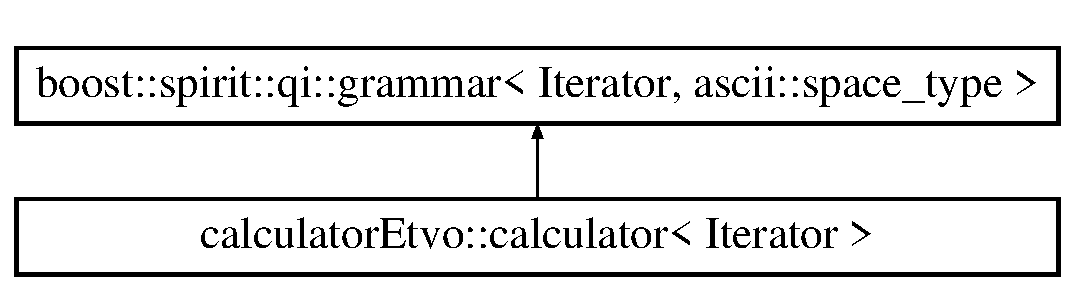
\includegraphics[height=2.000000cm]{structcalculator_etvo_1_1calculator}
\end{center}
\end{figure}
\subsection*{Public Attributes}
\begin{DoxyCompactItemize}
\item 
\mbox{\Hypertarget{structcalculator_etvo_1_1calculator_aeb809fd31fb429a4036d0246efa8c0a3}\label{structcalculator_etvo_1_1calculator_aeb809fd31fb429a4036d0246efa8c0a3}} 
qi\+::rule$<$ Iterator, ascii\+::space\+\_\+type $>$ {\bfseries statement}
\item 
\mbox{\Hypertarget{structcalculator_etvo_1_1calculator_a2fa5017612913058b3b43f6fad3773c7}\label{structcalculator_etvo_1_1calculator_a2fa5017612913058b3b43f6fad3773c7}} 
qi\+::rule$<$ Iterator, ascii\+::space\+\_\+type $>$ {\bfseries ev}
\item 
\mbox{\Hypertarget{structcalculator_etvo_1_1calculator_a0559f790e3950e00adf954df0f7af0e8}\label{structcalculator_etvo_1_1calculator_a0559f790e3950e00adf954df0f7af0e8}} 
qi\+::rule$<$ Iterator, ascii\+::space\+\_\+type $>$ {\bfseries expression\+Ed}
\item 
\mbox{\Hypertarget{structcalculator_etvo_1_1calculator_a607636f6ca0dfa332eaff309ae31afe0}\label{structcalculator_etvo_1_1calculator_a607636f6ca0dfa332eaff309ae31afe0}} 
qi\+::rule$<$ Iterator, ascii\+::space\+\_\+type $>$ {\bfseries inf\+Ed}
\item 
\mbox{\Hypertarget{structcalculator_etvo_1_1calculator_a04e25cab20ace8c27a4829d8ce9e96e6}\label{structcalculator_etvo_1_1calculator_a04e25cab20ace8c27a4829d8ce9e96e6}} 
qi\+::rule$<$ Iterator, ascii\+::space\+\_\+type $>$ {\bfseries lfrac\+Ed}
\item 
\mbox{\Hypertarget{structcalculator_etvo_1_1calculator_a8617083ed1d40f323392e599ae72f38e}\label{structcalculator_etvo_1_1calculator_a8617083ed1d40f323392e599ae72f38e}} 
qi\+::rule$<$ Iterator, ascii\+::space\+\_\+type $>$ {\bfseries rfrac\+Ed}
\item 
\mbox{\Hypertarget{structcalculator_etvo_1_1calculator_a988bc851dee4ed6e874708f78bc12993}\label{structcalculator_etvo_1_1calculator_a988bc851dee4ed6e874708f78bc12993}} 
qi\+::rule$<$ Iterator, ascii\+::space\+\_\+type $>$ {\bfseries prcaus\+Ed}
\item 
\mbox{\Hypertarget{structcalculator_etvo_1_1calculator_a69fc90d00ea5f1ce889e36e05d7749dd}\label{structcalculator_etvo_1_1calculator_a69fc90d00ea5f1ce889e36e05d7749dd}} 
qi\+::rule$<$ Iterator, ascii\+::space\+\_\+type $>$ {\bfseries right\+Ed}
\item 
\mbox{\Hypertarget{structcalculator_etvo_1_1calculator_a5ea0e4edd5c219636f27b68b1ae01104}\label{structcalculator_etvo_1_1calculator_a5ea0e4edd5c219636f27b68b1ae01104}} 
qi\+::rule$<$ Iterator, ascii\+::space\+\_\+type $>$ {\bfseries left\+Ed}
\item 
\mbox{\Hypertarget{structcalculator_etvo_1_1calculator_ab0f8965f74e8912eed5e297cc3cf4617}\label{structcalculator_etvo_1_1calculator_ab0f8965f74e8912eed5e297cc3cf4617}} 
qi\+::rule$<$ Iterator, ascii\+::space\+\_\+type $>$ {\bfseries M\+M\+To\+Ed}
\item 
\mbox{\Hypertarget{structcalculator_etvo_1_1calculator_aff49a0d056e905342bc9a981733d58ab}\label{structcalculator_etvo_1_1calculator_aff49a0d056e905342bc9a981733d58ab}} 
qi\+::rule$<$ Iterator, ascii\+::space\+\_\+type $>$ {\bfseries as\+Mu\+Var}
\item 
\mbox{\Hypertarget{structcalculator_etvo_1_1calculator_aa59a18a83b6f7efd1118b16af18604fb}\label{structcalculator_etvo_1_1calculator_aa59a18a83b6f7efd1118b16af18604fb}} 
qi\+::rule$<$ Iterator, ascii\+::space\+\_\+type $>$ {\bfseries factor\+Ed}
\item 
\mbox{\Hypertarget{structcalculator_etvo_1_1calculator_abb2bbd74c0fb200b1e4198aa94d33c8b}\label{structcalculator_etvo_1_1calculator_abb2bbd74c0fb200b1e4198aa94d33c8b}} 
qi\+::rule$<$ Iterator, ascii\+::space\+\_\+type $>$ {\bfseries group\+Ed}
\item 
\mbox{\Hypertarget{structcalculator_etvo_1_1calculator_afa1027ff41a729c4dec808fb423f1fef}\label{structcalculator_etvo_1_1calculator_afa1027ff41a729c4dec808fb423f1fef}} 
qi\+::rule$<$ Iterator, ascii\+::space\+\_\+type $>$ {\bfseries term\+Ed}
\item 
\mbox{\Hypertarget{structcalculator_etvo_1_1calculator_a46f213695a63ab1dda600e64088f5de7}\label{structcalculator_etvo_1_1calculator_a46f213695a63ab1dda600e64088f5de7}} 
qi\+::rule$<$ Iterator, ascii\+::space\+\_\+type $>$ {\bfseries poly\+Ed}
\item 
\mbox{\Hypertarget{structcalculator_etvo_1_1calculator_a4f32d19e49879b2b317cef1d102c76fd}\label{structcalculator_etvo_1_1calculator_a4f32d19e49879b2b317cef1d102c76fd}} 
qi\+::rule$<$ Iterator, ascii\+::space\+\_\+type $>$ {\bfseries nabla\+Ed}
\item 
\mbox{\Hypertarget{structcalculator_etvo_1_1calculator_abb1a048a718a91398e85f2395c8ceacb}\label{structcalculator_etvo_1_1calculator_abb1a048a718a91398e85f2395c8ceacb}} 
qi\+::rule$<$ Iterator, ascii\+::space\+\_\+type $>$ {\bfseries gamma\+Ed}
\item 
\mbox{\Hypertarget{structcalculator_etvo_1_1calculator_a012fbb8d7264f753ac5d90d08f9e58d9}\label{structcalculator_etvo_1_1calculator_a012fbb8d7264f753ac5d90d08f9e58d9}} 
qi\+::rule$<$ Iterator, ascii\+::space\+\_\+type $>$ {\bfseries seq\+Ed}
\item 
\mbox{\Hypertarget{structcalculator_etvo_1_1calculator_ae43df61896beb6c379311d1df1ab8ec2}\label{structcalculator_etvo_1_1calculator_ae43df61896beb6c379311d1df1ab8ec2}} 
qi\+::rule$<$ Iterator, ascii\+::space\+\_\+type $>$ {\bfseries mu\+Var\+Ed}
\item 
\mbox{\Hypertarget{structcalculator_etvo_1_1calculator_a668d32a18ee0d49c4fccf7c2bc75dfe8}\label{structcalculator_etvo_1_1calculator_a668d32a18ee0d49c4fccf7c2bc75dfe8}} 
qi\+::rule$<$ Iterator, ascii\+::space\+\_\+type $>$ {\bfseries beta\+Var\+Ed}
\item 
\mbox{\Hypertarget{structcalculator_etvo_1_1calculator_af6ec043bb5718d90fe0001497684a66f}\label{structcalculator_etvo_1_1calculator_af6ec043bb5718d90fe0001497684a66f}} 
qi\+::rule$<$ Iterator, ascii\+::space\+\_\+type $>$ {\bfseries equal\+Ed}
\item 
\mbox{\Hypertarget{structcalculator_etvo_1_1calculator_a8716e9e8256642de471529e6b411c486}\label{structcalculator_etvo_1_1calculator_a8716e9e8256642de471529e6b411c486}} 
qi\+::rule$<$ Iterator, ascii\+::space\+\_\+type $>$ {\bfseries as\+Core\+Ed}
\item 
\mbox{\Hypertarget{structcalculator_etvo_1_1calculator_a3e9e4e0874601a45a3d73496b54437ff}\label{structcalculator_etvo_1_1calculator_a3e9e4e0874601a45a3d73496b54437ff}} 
qi\+::rule$<$ Iterator, ascii\+::space\+\_\+type $>$ {\bfseries delta\+Ed}
\item 
\mbox{\Hypertarget{structcalculator_etvo_1_1calculator_a9347f5cd425b220238fdc8b5539ef814}\label{structcalculator_etvo_1_1calculator_a9347f5cd425b220238fdc8b5539ef814}} 
qi\+::rule$<$ Iterator, ascii\+::space\+\_\+type $>$ {\bfseries mu\+Ed}
\item 
\mbox{\Hypertarget{structcalculator_etvo_1_1calculator_a2fed4f985f9433d9f558fa23bdd20389}\label{structcalculator_etvo_1_1calculator_a2fed4f985f9433d9f558fa23bdd20389}} 
qi\+::rule$<$ Iterator, ascii\+::space\+\_\+type $>$ {\bfseries beta\+Ed}
\item 
\mbox{\Hypertarget{structcalculator_etvo_1_1calculator_af15e3b55521beb4b710e8919c2edc7d4}\label{structcalculator_etvo_1_1calculator_af15e3b55521beb4b710e8919c2edc7d4}} 
qi\+::rule$<$ Iterator, ascii\+::space\+\_\+type $>$ {\bfseries eps\+Ed}
\item 
\mbox{\Hypertarget{structcalculator_etvo_1_1calculator_a9460f35ba4420cbff06ebabeadefa70e}\label{structcalculator_etvo_1_1calculator_a9460f35ba4420cbff06ebabeadefa70e}} 
qi\+::rule$<$ Iterator, ascii\+::space\+\_\+type $>$ {\bfseries kleene\+Ed}
\item 
\mbox{\Hypertarget{structcalculator_etvo_1_1calculator_a79ac46378c7ffc24d2d0d0a11f83cc55}\label{structcalculator_etvo_1_1calculator_a79ac46378c7ffc24d2d0d0a11f83cc55}} 
qi\+::rule$<$ Iterator, ascii\+::space\+\_\+type $>$ {\bfseries ident\+Ed}
\item 
\mbox{\Hypertarget{structcalculator_etvo_1_1calculator_ae29f48db5abeb54b5fa3e447a1ee3cb6}\label{structcalculator_etvo_1_1calculator_ae29f48db5abeb54b5fa3e447a1ee3cb6}} 
qi\+::rule$<$ Iterator, ascii\+::space\+\_\+type $>$ {\bfseries assign\+Ed}
\item 
\mbox{\Hypertarget{structcalculator_etvo_1_1calculator_aac2c0edb6da3ef901146b5d80df8ccdf}\label{structcalculator_etvo_1_1calculator_aac2c0edb6da3ef901146b5d80df8ccdf}} 
qi\+::rule$<$ Iterator, ascii\+::space\+\_\+type $>$ {\bfseries expression\+MM}
\item 
\mbox{\Hypertarget{structcalculator_etvo_1_1calculator_a44f76720fa0c791479e6ff9ea177ea36}\label{structcalculator_etvo_1_1calculator_a44f76720fa0c791479e6ff9ea177ea36}} 
qi\+::rule$<$ Iterator, ascii\+::space\+\_\+type $>$ {\bfseries mm}
\item 
\mbox{\Hypertarget{structcalculator_etvo_1_1calculator_a57981d3466c2d1fa6e07341e15c7e145}\label{structcalculator_etvo_1_1calculator_a57981d3466c2d1fa6e07341e15c7e145}} 
qi\+::rule$<$ Iterator, ascii\+::space\+\_\+type $>$ {\bfseries gamma\+MM}
\item 
\mbox{\Hypertarget{structcalculator_etvo_1_1calculator_a27331245db72c81e8de55ae9816814a8}\label{structcalculator_etvo_1_1calculator_a27331245db72c81e8de55ae9816814a8}} 
qi\+::rule$<$ Iterator, ascii\+::space\+\_\+type $>$ {\bfseries delta\+MM}
\item 
\mbox{\Hypertarget{structcalculator_etvo_1_1calculator_af8d6c1a6fc9b8b64099f8592a11e7f16}\label{structcalculator_etvo_1_1calculator_af8d6c1a6fc9b8b64099f8592a11e7f16}} 
qi\+::rule$<$ Iterator, ascii\+::space\+\_\+type $>$ {\bfseries inf\+MM}
\item 
\mbox{\Hypertarget{structcalculator_etvo_1_1calculator_ad53aaf1f95058e74cf7f2f886bec1a15}\label{structcalculator_etvo_1_1calculator_ad53aaf1f95058e74cf7f2f886bec1a15}} 
qi\+::rule$<$ Iterator, ascii\+::space\+\_\+type $>$ {\bfseries frac\+MM}
\item 
\mbox{\Hypertarget{structcalculator_etvo_1_1calculator_a51920b7cc686d516fa1d9a518224d97d}\label{structcalculator_etvo_1_1calculator_a51920b7cc686d516fa1d9a518224d97d}} 
qi\+::rule$<$ Iterator, ascii\+::space\+\_\+type $>$ {\bfseries prcaus\+MM}
\item 
\mbox{\Hypertarget{structcalculator_etvo_1_1calculator_ac352ab017168124f4dedb66b38f30c6c}\label{structcalculator_etvo_1_1calculator_ac352ab017168124f4dedb66b38f30c6c}} 
qi\+::rule$<$ Iterator, ascii\+::space\+\_\+type $>$ {\bfseries Ed\+To\+MM}
\item 
\mbox{\Hypertarget{structcalculator_etvo_1_1calculator_aff27171330307206e88e90231a26370d}\label{structcalculator_etvo_1_1calculator_aff27171330307206e88e90231a26370d}} 
qi\+::rule$<$ Iterator, ascii\+::space\+\_\+type $>$ {\bfseries Tg\+To\+MM}
\item 
\mbox{\Hypertarget{structcalculator_etvo_1_1calculator_aecc67b4ee3f24e5d4d3e8fad49169eda}\label{structcalculator_etvo_1_1calculator_aecc67b4ee3f24e5d4d3e8fad49169eda}} 
qi\+::rule$<$ Iterator, ascii\+::space\+\_\+type $>$ {\bfseries equal\+MM}
\item 
\mbox{\Hypertarget{structcalculator_etvo_1_1calculator_a615ba8202e2a43e3a036f86b6202a4f7}\label{structcalculator_etvo_1_1calculator_a615ba8202e2a43e3a036f86b6202a4f7}} 
qi\+::rule$<$ Iterator, ascii\+::space\+\_\+type $>$ {\bfseries factor\+MM}
\item 
\mbox{\Hypertarget{structcalculator_etvo_1_1calculator_a0cdef6b09c6bd8a8de6242f66c280b60}\label{structcalculator_etvo_1_1calculator_a0cdef6b09c6bd8a8de6242f66c280b60}} 
qi\+::rule$<$ Iterator, ascii\+::space\+\_\+type $>$ {\bfseries group\+MM}
\item 
\mbox{\Hypertarget{structcalculator_etvo_1_1calculator_a80d0c260fb01f42d7c51c3ff210a4159}\label{structcalculator_etvo_1_1calculator_a80d0c260fb01f42d7c51c3ff210a4159}} 
qi\+::rule$<$ Iterator, ascii\+::space\+\_\+type $>$ {\bfseries term\+MM}
\item 
\mbox{\Hypertarget{structcalculator_etvo_1_1calculator_ab8306a14a281c79f1125f0e3b34a3a16}\label{structcalculator_etvo_1_1calculator_ab8306a14a281c79f1125f0e3b34a3a16}} 
qi\+::rule$<$ Iterator, ascii\+::space\+\_\+type $>$ {\bfseries poly\+MM}
\item 
\mbox{\Hypertarget{structcalculator_etvo_1_1calculator_a4efe854338e4e6e671bbf726be9db261}\label{structcalculator_etvo_1_1calculator_a4efe854338e4e6e671bbf726be9db261}} 
qi\+::rule$<$ Iterator, ascii\+::space\+\_\+type $>$ {\bfseries eps\+MM}
\item 
\mbox{\Hypertarget{structcalculator_etvo_1_1calculator_a6182756543d6e3dd7bd2834c321f7b09}\label{structcalculator_etvo_1_1calculator_a6182756543d6e3dd7bd2834c321f7b09}} 
qi\+::rule$<$ Iterator, ascii\+::space\+\_\+type $>$ {\bfseries kleene\+MM}
\item 
\mbox{\Hypertarget{structcalculator_etvo_1_1calculator_a5153c027576848fc52f5d8d15e27f75c}\label{structcalculator_etvo_1_1calculator_a5153c027576848fc52f5d8d15e27f75c}} 
qi\+::rule$<$ Iterator, ascii\+::space\+\_\+type $>$ {\bfseries ident\+MM}
\item 
\mbox{\Hypertarget{structcalculator_etvo_1_1calculator_af00637d056fd556568b4c095fabeae0c}\label{structcalculator_etvo_1_1calculator_af00637d056fd556568b4c095fabeae0c}} 
qi\+::rule$<$ Iterator, ascii\+::space\+\_\+type $>$ {\bfseries assign\+MM}
\item 
\mbox{\Hypertarget{structcalculator_etvo_1_1calculator_a29bde4b6d9501c3ae70e2b4ee3898141}\label{structcalculator_etvo_1_1calculator_a29bde4b6d9501c3ae70e2b4ee3898141}} 
qi\+::rule$<$ Iterator, ascii\+::space\+\_\+type $>$ {\bfseries expression\+Tg}
\item 
\mbox{\Hypertarget{structcalculator_etvo_1_1calculator_a719cc2ee8d7034b120b35cc2f2448597}\label{structcalculator_etvo_1_1calculator_a719cc2ee8d7034b120b35cc2f2448597}} 
qi\+::rule$<$ Iterator, ascii\+::space\+\_\+type $>$ {\bfseries tv}
\item 
\mbox{\Hypertarget{structcalculator_etvo_1_1calculator_a830c98c94ec448f7d26c495d79de7034}\label{structcalculator_etvo_1_1calculator_a830c98c94ec448f7d26c495d79de7034}} 
qi\+::rule$<$ Iterator, ascii\+::space\+\_\+type $>$ {\bfseries inf\+Tg}
\item 
\mbox{\Hypertarget{structcalculator_etvo_1_1calculator_a430020791d760fea756b2c6dd5567db1}\label{structcalculator_etvo_1_1calculator_a430020791d760fea756b2c6dd5567db1}} 
qi\+::rule$<$ Iterator, ascii\+::space\+\_\+type $>$ {\bfseries lfrac\+Tg}
\item 
\mbox{\Hypertarget{structcalculator_etvo_1_1calculator_a2ce177b720431ba76926ed281424e9a8}\label{structcalculator_etvo_1_1calculator_a2ce177b720431ba76926ed281424e9a8}} 
qi\+::rule$<$ Iterator, ascii\+::space\+\_\+type $>$ {\bfseries rfrac\+Tg}
\item 
\mbox{\Hypertarget{structcalculator_etvo_1_1calculator_a088cf29b4b40b878e355a426615d73dd}\label{structcalculator_etvo_1_1calculator_a088cf29b4b40b878e355a426615d73dd}} 
qi\+::rule$<$ Iterator, ascii\+::space\+\_\+type $>$ {\bfseries prcaus\+Tg}
\item 
\mbox{\Hypertarget{structcalculator_etvo_1_1calculator_a94433b60268bb7c067efce17787c3ea6}\label{structcalculator_etvo_1_1calculator_a94433b60268bb7c067efce17787c3ea6}} 
qi\+::rule$<$ Iterator, ascii\+::space\+\_\+type $>$ {\bfseries right\+Tg}
\item 
\mbox{\Hypertarget{structcalculator_etvo_1_1calculator_a9376ef9e6487392a9cc9569801b0edc4}\label{structcalculator_etvo_1_1calculator_a9376ef9e6487392a9cc9569801b0edc4}} 
qi\+::rule$<$ Iterator, ascii\+::space\+\_\+type $>$ {\bfseries left\+Tg}
\item 
\mbox{\Hypertarget{structcalculator_etvo_1_1calculator_a78b46537d6e8644bacf7ef7aff44b01d}\label{structcalculator_etvo_1_1calculator_a78b46537d6e8644bacf7ef7aff44b01d}} 
qi\+::rule$<$ Iterator, ascii\+::space\+\_\+type $>$ {\bfseries gamma\+Tg}
\item 
\mbox{\Hypertarget{structcalculator_etvo_1_1calculator_acb26b00e092bfc54764e96004b4bdadd}\label{structcalculator_etvo_1_1calculator_acb26b00e092bfc54764e96004b4bdadd}} 
qi\+::rule$<$ Iterator, ascii\+::space\+\_\+type $>$ {\bfseries delta\+Tg}
\item 
\mbox{\Hypertarget{structcalculator_etvo_1_1calculator_a867dfe99cfdea151d2e8bbc9a092242f}\label{structcalculator_etvo_1_1calculator_a867dfe99cfdea151d2e8bbc9a092242f}} 
qi\+::rule$<$ Iterator, ascii\+::space\+\_\+type $>$ {\bfseries Delta\+Tg}
\item 
\mbox{\Hypertarget{structcalculator_etvo_1_1calculator_a34773bac880f02d076f85dce25e8944a}\label{structcalculator_etvo_1_1calculator_a34773bac880f02d076f85dce25e8944a}} 
qi\+::rule$<$ Iterator, ascii\+::space\+\_\+type $>$ {\bfseries M\+M\+To\+Tg}
\item 
\mbox{\Hypertarget{structcalculator_etvo_1_1calculator_a5888f730e04cf524c296f53a6110fdf3}\label{structcalculator_etvo_1_1calculator_a5888f730e04cf524c296f53a6110fdf3}} 
qi\+::rule$<$ Iterator, ascii\+::space\+\_\+type $>$ {\bfseries factor\+Tg}
\item 
\mbox{\Hypertarget{structcalculator_etvo_1_1calculator_a51ba7b2938552f7565cfad74aa110403}\label{structcalculator_etvo_1_1calculator_a51ba7b2938552f7565cfad74aa110403}} 
qi\+::rule$<$ Iterator, ascii\+::space\+\_\+type $>$ {\bfseries group\+Tg}
\item 
\mbox{\Hypertarget{structcalculator_etvo_1_1calculator_a183b70fc36f2f93da9e0e014aeb37764}\label{structcalculator_etvo_1_1calculator_a183b70fc36f2f93da9e0e014aeb37764}} 
qi\+::rule$<$ Iterator, ascii\+::space\+\_\+type $>$ {\bfseries term\+Tg}
\item 
\mbox{\Hypertarget{structcalculator_etvo_1_1calculator_a20fb97055e0f86045fd0e8fd6df1bfb9}\label{structcalculator_etvo_1_1calculator_a20fb97055e0f86045fd0e8fd6df1bfb9}} 
qi\+::rule$<$ Iterator, ascii\+::space\+\_\+type $>$ {\bfseries poly\+Tg}
\item 
\mbox{\Hypertarget{structcalculator_etvo_1_1calculator_a23bd743a243f2f5af1ac12f1e5cc6dcc}\label{structcalculator_etvo_1_1calculator_a23bd743a243f2f5af1ac12f1e5cc6dcc}} 
qi\+::rule$<$ Iterator, ascii\+::space\+\_\+type $>$ {\bfseries eps\+Tg}
\item 
\mbox{\Hypertarget{structcalculator_etvo_1_1calculator_af39c11f4c9ea1f78752c9a89953d13c3}\label{structcalculator_etvo_1_1calculator_af39c11f4c9ea1f78752c9a89953d13c3}} 
qi\+::rule$<$ Iterator, ascii\+::space\+\_\+type $>$ {\bfseries kleene\+Tg}
\item 
\mbox{\Hypertarget{structcalculator_etvo_1_1calculator_a71a58b97998a33c024ce250d7055779e}\label{structcalculator_etvo_1_1calculator_a71a58b97998a33c024ce250d7055779e}} 
qi\+::rule$<$ Iterator, ascii\+::space\+\_\+type $>$ {\bfseries ident\+Tg}
\item 
\mbox{\Hypertarget{structcalculator_etvo_1_1calculator_a05a6608a64eed7eca37f3cf267c1e813}\label{structcalculator_etvo_1_1calculator_a05a6608a64eed7eca37f3cf267c1e813}} 
qi\+::rule$<$ Iterator, ascii\+::space\+\_\+type $>$ {\bfseries assign\+Tg}
\item 
\mbox{\Hypertarget{structcalculator_etvo_1_1calculator_acf4d6c84c7130e2bf64b9f650452d625}\label{structcalculator_etvo_1_1calculator_acf4d6c84c7130e2bf64b9f650452d625}} 
qi\+::rule$<$ Iterator, ascii\+::space\+\_\+type $>$ {\bfseries delta\+Var\+Tg}
\item 
\mbox{\Hypertarget{structcalculator_etvo_1_1calculator_afe6e95609570c818f6b05b9123ef9998}\label{structcalculator_etvo_1_1calculator_afe6e95609570c818f6b05b9123ef9998}} 
qi\+::rule$<$ Iterator, ascii\+::space\+\_\+type $>$ {\bfseries seq\+Tg}
\item 
\mbox{\Hypertarget{structcalculator_etvo_1_1calculator_acb6c729d98372ba07bc1c99ffc4c3d38}\label{structcalculator_etvo_1_1calculator_acb6c729d98372ba07bc1c99ffc4c3d38}} 
qi\+::rule$<$ Iterator, ascii\+::space\+\_\+type $>$ {\bfseries equal\+Tg}
\item 
\mbox{\Hypertarget{structcalculator_etvo_1_1calculator_abf09a1c1c233449b083ec03aa05e3a72}\label{structcalculator_etvo_1_1calculator_abf09a1c1c233449b083ec03aa05e3a72}} 
qi\+::rule$<$ Iterator, ascii\+::space\+\_\+type $>$ {\bfseries as\+Delta\+Var}
\item 
\mbox{\Hypertarget{structcalculator_etvo_1_1calculator_a211157350e38a3d60b7a247214e9e3bc}\label{structcalculator_etvo_1_1calculator_a211157350e38a3d60b7a247214e9e3bc}} 
qi\+::rule$<$ Iterator, ascii\+::space\+\_\+type $>$ {\bfseries as\+Core\+Tg}
\end{DoxyCompactItemize}


The documentation for this struct was generated from the following file\+:\begin{DoxyCompactItemize}
\item 
etvo/parsers/calculator.\+cpp\end{DoxyCompactItemize}

\hypertarget{structparseseriesed_1_1calculator}{}\section{parseseriesed\+:\+:calculator$<$ Iterator $>$ Struct Template Reference}
\label{structparseseriesed_1_1calculator}\index{parseseriesed\+::calculator$<$ Iterator $>$@{parseseriesed\+::calculator$<$ Iterator $>$}}
Inheritance diagram for parseseriesed\+:\+:calculator$<$ Iterator $>$\+:\begin{figure}[H]
\begin{center}
\leavevmode
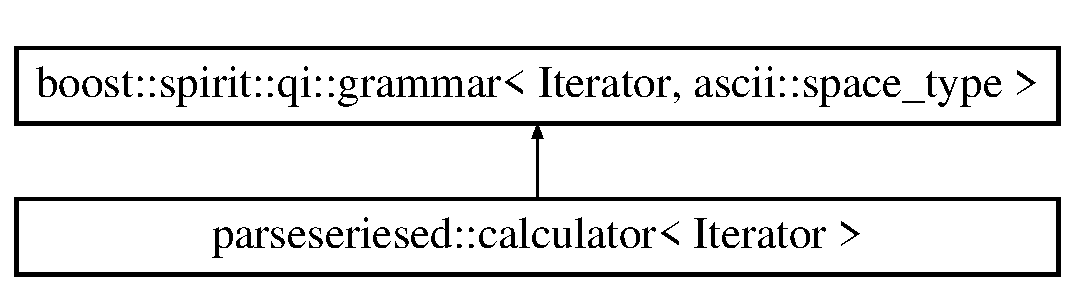
\includegraphics[height=2.000000cm]{structparseseriesed_1_1calculator}
\end{center}
\end{figure}
\subsection*{Public Attributes}
\begin{DoxyCompactItemize}
\item 
\mbox{\Hypertarget{structparseseriesed_1_1calculator_afbb52858bdfeda8fe33634a284f99aae}\label{structparseseriesed_1_1calculator_afbb52858bdfeda8fe33634a284f99aae}} 
qi\+::rule$<$ Iterator, ascii\+::space\+\_\+type $>$ {\bfseries statement}
\item 
\mbox{\Hypertarget{structparseseriesed_1_1calculator_a12755dbe77a1f4b01953e958689297cc}\label{structparseseriesed_1_1calculator_a12755dbe77a1f4b01953e958689297cc}} 
qi\+::rule$<$ Iterator, ascii\+::space\+\_\+type $>$ {\bfseries expression}
\item 
\mbox{\Hypertarget{structparseseriesed_1_1calculator_aa0ba1d9bbefbdef23b444bbce85a9950}\label{structparseseriesed_1_1calculator_aa0ba1d9bbefbdef23b444bbce85a9950}} 
qi\+::rule$<$ Iterator, ascii\+::space\+\_\+type $>$ {\bfseries factor}
\item 
\mbox{\Hypertarget{structparseseriesed_1_1calculator_a9ca16a3fe105eacb0c0f9ad5537cab7e}\label{structparseseriesed_1_1calculator_a9ca16a3fe105eacb0c0f9ad5537cab7e}} 
qi\+::rule$<$ Iterator, ascii\+::space\+\_\+type $>$ {\bfseries group}
\item 
\mbox{\Hypertarget{structparseseriesed_1_1calculator_a3090010544328d356e8daa12c150304b}\label{structparseseriesed_1_1calculator_a3090010544328d356e8daa12c150304b}} 
qi\+::rule$<$ Iterator, ascii\+::space\+\_\+type $>$ {\bfseries term}
\item 
\mbox{\Hypertarget{structparseseriesed_1_1calculator_a3fe87fe72cc305941229f2a07b912d87}\label{structparseseriesed_1_1calculator_a3fe87fe72cc305941229f2a07b912d87}} 
qi\+::rule$<$ Iterator, ascii\+::space\+\_\+type $>$ {\bfseries poly}
\item 
\mbox{\Hypertarget{structparseseriesed_1_1calculator_af8ddd3d404a8959f65ef3fd31344c978}\label{structparseseriesed_1_1calculator_af8ddd3d404a8959f65ef3fd31344c978}} 
qi\+::rule$<$ Iterator, ascii\+::space\+\_\+type $>$ {\bfseries nabla}
\item 
\mbox{\Hypertarget{structparseseriesed_1_1calculator_a2c069daeb82d9cccd8e3a1c0544ae59a}\label{structparseseriesed_1_1calculator_a2c069daeb82d9cccd8e3a1c0544ae59a}} 
qi\+::rule$<$ Iterator, ascii\+::space\+\_\+type $>$ {\bfseries gamma}
\item 
\mbox{\Hypertarget{structparseseriesed_1_1calculator_a829f802f5e0e84ed5fb1e7a2ae9a73dc}\label{structparseseriesed_1_1calculator_a829f802f5e0e84ed5fb1e7a2ae9a73dc}} 
qi\+::rule$<$ Iterator, ascii\+::space\+\_\+type $>$ {\bfseries delta}
\item 
\mbox{\Hypertarget{structparseseriesed_1_1calculator_a4124d1a64af9871e2c65d13c4593ddad}\label{structparseseriesed_1_1calculator_a4124d1a64af9871e2c65d13c4593ddad}} 
qi\+::rule$<$ Iterator, ascii\+::space\+\_\+type $>$ {\bfseries mu}
\item 
\mbox{\Hypertarget{structparseseriesed_1_1calculator_a84db848763cf5b78e6939a98af34ea50}\label{structparseseriesed_1_1calculator_a84db848763cf5b78e6939a98af34ea50}} 
qi\+::rule$<$ Iterator, ascii\+::space\+\_\+type $>$ {\bfseries beta}
\item 
\mbox{\Hypertarget{structparseseriesed_1_1calculator_ae716a0e0be96d22be033a01607b29dcc}\label{structparseseriesed_1_1calculator_ae716a0e0be96d22be033a01607b29dcc}} 
qi\+::rule$<$ Iterator, ascii\+::space\+\_\+type $>$ {\bfseries kleene}
\end{DoxyCompactItemize}


The documentation for this struct was generated from the following file\+:\begin{DoxyCompactItemize}
\item 
etvo/parsers/parser\+Series\+Ed.\+cpp\end{DoxyCompactItemize}

\hypertarget{structparseped_1_1calculator}{}\section{parseped\+:\+:calculator$<$ Iterator $>$ Struct Template Reference}
\label{structparseped_1_1calculator}\index{parseped\+::calculator$<$ Iterator $>$@{parseped\+::calculator$<$ Iterator $>$}}
Inheritance diagram for parseped\+:\+:calculator$<$ Iterator $>$\+:\begin{figure}[H]
\begin{center}
\leavevmode
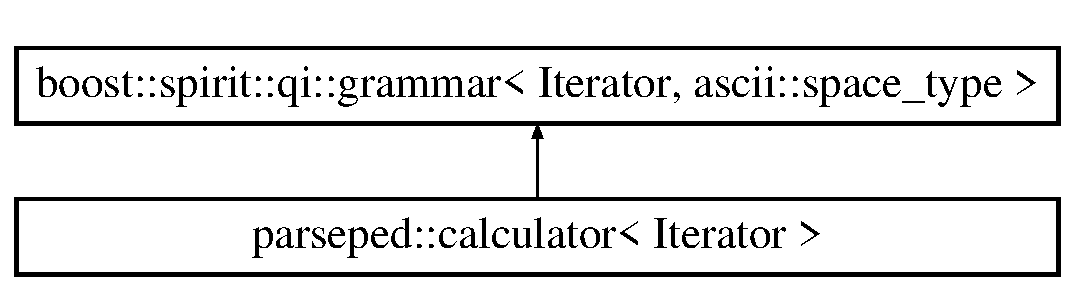
\includegraphics[height=2.000000cm]{structparseped_1_1calculator}
\end{center}
\end{figure}
\subsection*{Public Attributes}
\begin{DoxyCompactItemize}
\item 
\mbox{\Hypertarget{structparseped_1_1calculator_ab46d9b24fa79188d1a922a8e9f08d792}\label{structparseped_1_1calculator_ab46d9b24fa79188d1a922a8e9f08d792}} 
qi\+::rule$<$ Iterator, ascii\+::space\+\_\+type $>$ {\bfseries statement}
\item 
\mbox{\Hypertarget{structparseped_1_1calculator_a908d152da6ba5c5029fbc3ff4828a8b9}\label{structparseped_1_1calculator_a908d152da6ba5c5029fbc3ff4828a8b9}} 
qi\+::rule$<$ Iterator, ascii\+::space\+\_\+type $>$ {\bfseries expression}
\item 
\mbox{\Hypertarget{structparseped_1_1calculator_a7b00996c7b94579f09ef24b82e010a30}\label{structparseped_1_1calculator_a7b00996c7b94579f09ef24b82e010a30}} 
qi\+::rule$<$ Iterator, ascii\+::space\+\_\+type $>$ {\bfseries factor}
\item 
\mbox{\Hypertarget{structparseped_1_1calculator_a0bc97d6be1c040150a8dc66c5c44827a}\label{structparseped_1_1calculator_a0bc97d6be1c040150a8dc66c5c44827a}} 
qi\+::rule$<$ Iterator, ascii\+::space\+\_\+type $>$ {\bfseries group}
\item 
\mbox{\Hypertarget{structparseped_1_1calculator_a800f65823e037adb4d2acbd6ae560cd2}\label{structparseped_1_1calculator_a800f65823e037adb4d2acbd6ae560cd2}} 
qi\+::rule$<$ Iterator, ascii\+::space\+\_\+type $>$ {\bfseries term}
\item 
\mbox{\Hypertarget{structparseped_1_1calculator_a7cf1b97fe7e3097627734c89fe1241b2}\label{structparseped_1_1calculator_a7cf1b97fe7e3097627734c89fe1241b2}} 
qi\+::rule$<$ Iterator, ascii\+::space\+\_\+type $>$ {\bfseries poly}
\item 
\mbox{\Hypertarget{structparseped_1_1calculator_aad1491bb321232952f1a99bfe0ee3fa9}\label{structparseped_1_1calculator_aad1491bb321232952f1a99bfe0ee3fa9}} 
qi\+::rule$<$ Iterator, ascii\+::space\+\_\+type $>$ {\bfseries nabla}
\item 
\mbox{\Hypertarget{structparseped_1_1calculator_a29131c7c62893a894238965347125a04}\label{structparseped_1_1calculator_a29131c7c62893a894238965347125a04}} 
qi\+::rule$<$ Iterator, ascii\+::space\+\_\+type $>$ {\bfseries gamma}
\item 
\mbox{\Hypertarget{structparseped_1_1calculator_a62e78884259bdc822bf1693f7ead10c6}\label{structparseped_1_1calculator_a62e78884259bdc822bf1693f7ead10c6}} 
qi\+::rule$<$ Iterator, ascii\+::space\+\_\+type $>$ {\bfseries delta}
\item 
\mbox{\Hypertarget{structparseped_1_1calculator_a56e06ab194908855f63b09fc8d4eb57f}\label{structparseped_1_1calculator_a56e06ab194908855f63b09fc8d4eb57f}} 
qi\+::rule$<$ Iterator, ascii\+::space\+\_\+type $>$ {\bfseries mu}
\item 
\mbox{\Hypertarget{structparseped_1_1calculator_a3f6b58fbe01c4f3d93a3d2e8716674be}\label{structparseped_1_1calculator_a3f6b58fbe01c4f3d93a3d2e8716674be}} 
qi\+::rule$<$ Iterator, ascii\+::space\+\_\+type $>$ {\bfseries beta}
\end{DoxyCompactItemize}


The documentation for this struct was generated from the following file\+:\begin{DoxyCompactItemize}
\item 
etvo/parsers/parser.\+cpp\end{DoxyCompactItemize}

\hypertarget{structparseptg_1_1calculator}{}\section{parseptg\+:\+:calculator$<$ Iterator $>$ Struct Template Reference}
\label{structparseptg_1_1calculator}\index{parseptg\+::calculator$<$ Iterator $>$@{parseptg\+::calculator$<$ Iterator $>$}}
Inheritance diagram for parseptg\+:\+:calculator$<$ Iterator $>$\+:\begin{figure}[H]
\begin{center}
\leavevmode
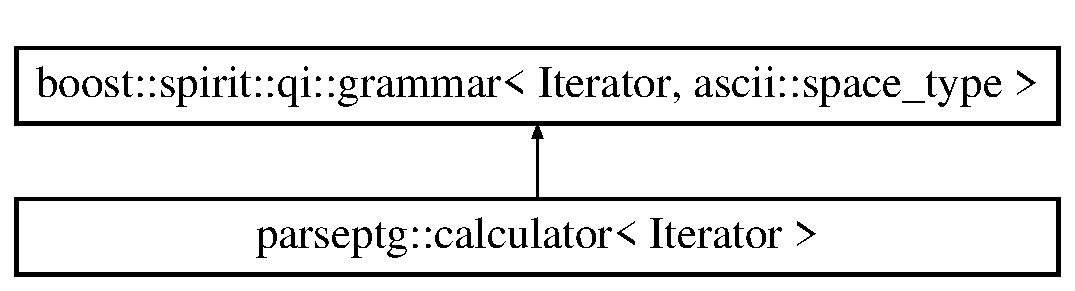
\includegraphics[height=2.000000cm]{structparseptg_1_1calculator}
\end{center}
\end{figure}
\subsection*{Public Attributes}
\begin{DoxyCompactItemize}
\item 
\mbox{\Hypertarget{structparseptg_1_1calculator_a53fdb55e2e860d17fcd42bf20129a5e7}\label{structparseptg_1_1calculator_a53fdb55e2e860d17fcd42bf20129a5e7}} 
qi\+::rule$<$ Iterator, ascii\+::space\+\_\+type $>$ {\bfseries statement}
\item 
\mbox{\Hypertarget{structparseptg_1_1calculator_a2142525e58cfcbe60bff5e57fade375a}\label{structparseptg_1_1calculator_a2142525e58cfcbe60bff5e57fade375a}} 
qi\+::rule$<$ Iterator, ascii\+::space\+\_\+type $>$ {\bfseries expression}
\item 
\mbox{\Hypertarget{structparseptg_1_1calculator_afde38ac64ef71f3107194a8ebef12ebf}\label{structparseptg_1_1calculator_afde38ac64ef71f3107194a8ebef12ebf}} 
qi\+::rule$<$ Iterator, ascii\+::space\+\_\+type $>$ {\bfseries factor}
\item 
\mbox{\Hypertarget{structparseptg_1_1calculator_abc10ee28c6611f001d682ee0dec3a236}\label{structparseptg_1_1calculator_abc10ee28c6611f001d682ee0dec3a236}} 
qi\+::rule$<$ Iterator, ascii\+::space\+\_\+type $>$ {\bfseries group}
\item 
\mbox{\Hypertarget{structparseptg_1_1calculator_a275331a2b5012b1fa282e13c5c278297}\label{structparseptg_1_1calculator_a275331a2b5012b1fa282e13c5c278297}} 
qi\+::rule$<$ Iterator, ascii\+::space\+\_\+type $>$ {\bfseries term}
\item 
\mbox{\Hypertarget{structparseptg_1_1calculator_a521dd00ceeb3839f1080f175f115c9ef}\label{structparseptg_1_1calculator_a521dd00ceeb3839f1080f175f115c9ef}} 
qi\+::rule$<$ Iterator, ascii\+::space\+\_\+type $>$ {\bfseries poly}
\item 
\mbox{\Hypertarget{structparseptg_1_1calculator_aaad87741e619d05ad584a29ca40a0b1a}\label{structparseptg_1_1calculator_aaad87741e619d05ad584a29ca40a0b1a}} 
qi\+::rule$<$ Iterator, ascii\+::space\+\_\+type $>$ {\bfseries D\+E\+L\+TA}
\item 
\mbox{\Hypertarget{structparseptg_1_1calculator_a5011dc3c707b95a3b3173f945740a730}\label{structparseptg_1_1calculator_a5011dc3c707b95a3b3173f945740a730}} 
qi\+::rule$<$ Iterator, ascii\+::space\+\_\+type $>$ {\bfseries gamma}
\item 
\mbox{\Hypertarget{structparseptg_1_1calculator_af4d4ed2e90c85f166ffc2c84bb38c376}\label{structparseptg_1_1calculator_af4d4ed2e90c85f166ffc2c84bb38c376}} 
qi\+::rule$<$ Iterator, ascii\+::space\+\_\+type $>$ {\bfseries delta}
\end{DoxyCompactItemize}


The documentation for this struct was generated from the following file\+:\begin{DoxyCompactItemize}
\item 
etvo/parsers/parser.\+cpp\end{DoxyCompactItemize}

\hypertarget{structparsepoly_i_i_i_1_1calculator}{}\section{parsepoly\+I\+II\+:\+:calculator$<$ Iterator $>$ Struct Template Reference}
\label{structparsepoly_i_i_i_1_1calculator}\index{parsepoly\+I\+I\+I\+::calculator$<$ Iterator $>$@{parsepoly\+I\+I\+I\+::calculator$<$ Iterator $>$}}
Inheritance diagram for parsepoly\+I\+II\+:\+:calculator$<$ Iterator $>$\+:\begin{figure}[H]
\begin{center}
\leavevmode
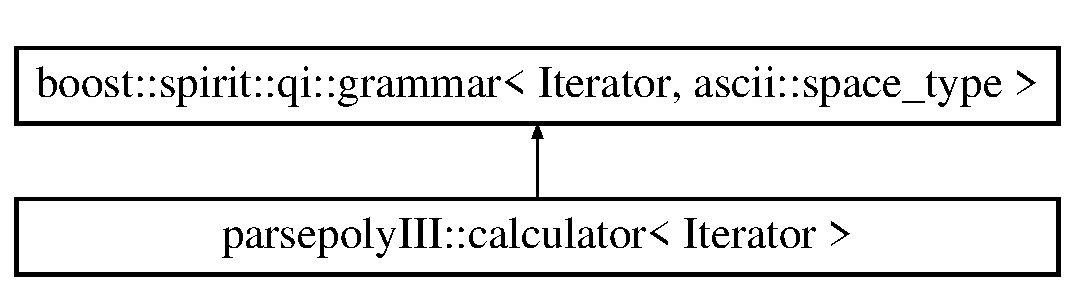
\includegraphics[height=2.000000cm]{structparsepoly_i_i_i_1_1calculator}
\end{center}
\end{figure}
\subsection*{Public Attributes}
\begin{DoxyCompactItemize}
\item 
\mbox{\Hypertarget{structparsepoly_i_i_i_1_1calculator_ac4d1630760c1a5dd42530359e7745fac}\label{structparsepoly_i_i_i_1_1calculator_ac4d1630760c1a5dd42530359e7745fac}} 
qi\+::rule$<$ Iterator, ascii\+::space\+\_\+type $>$ {\bfseries statement}
\item 
\mbox{\Hypertarget{structparsepoly_i_i_i_1_1calculator_acf9256c63c2d22fb796b60546d7afab7}\label{structparsepoly_i_i_i_1_1calculator_acf9256c63c2d22fb796b60546d7afab7}} 
qi\+::rule$<$ Iterator, ascii\+::space\+\_\+type $>$ {\bfseries expression}
\item 
\mbox{\Hypertarget{structparsepoly_i_i_i_1_1calculator_a0ee412204b1c723e26cf9d4d38ea23f0}\label{structparsepoly_i_i_i_1_1calculator_a0ee412204b1c723e26cf9d4d38ea23f0}} 
qi\+::rule$<$ Iterator, ascii\+::space\+\_\+type $>$ {\bfseries factor}
\item 
\mbox{\Hypertarget{structparsepoly_i_i_i_1_1calculator_a9094537b17e7894ac0a1f5940a80630a}\label{structparsepoly_i_i_i_1_1calculator_a9094537b17e7894ac0a1f5940a80630a}} 
qi\+::rule$<$ Iterator, ascii\+::space\+\_\+type $>$ {\bfseries group}
\item 
\mbox{\Hypertarget{structparsepoly_i_i_i_1_1calculator_a71a60be08388b36e22971d47817c3815}\label{structparsepoly_i_i_i_1_1calculator_a71a60be08388b36e22971d47817c3815}} 
qi\+::rule$<$ Iterator, ascii\+::space\+\_\+type $>$ {\bfseries term}
\item 
\mbox{\Hypertarget{structparsepoly_i_i_i_1_1calculator_ad217b4cf3123379b5ff80f5cacea1422}\label{structparsepoly_i_i_i_1_1calculator_ad217b4cf3123379b5ff80f5cacea1422}} 
qi\+::rule$<$ Iterator, ascii\+::space\+\_\+type $>$ {\bfseries poly}
\item 
\mbox{\Hypertarget{structparsepoly_i_i_i_1_1calculator_a5e97dd49cd73b13c9bd1fe50344a8014}\label{structparsepoly_i_i_i_1_1calculator_a5e97dd49cd73b13c9bd1fe50344a8014}} 
qi\+::rule$<$ Iterator, ascii\+::space\+\_\+type $>$ {\bfseries gamma}
\item 
\mbox{\Hypertarget{structparsepoly_i_i_i_1_1calculator_a1fb43c883186e7ad87107bfb78029c29}\label{structparsepoly_i_i_i_1_1calculator_a1fb43c883186e7ad87107bfb78029c29}} 
qi\+::rule$<$ Iterator, ascii\+::space\+\_\+type $>$ {\bfseries delta}
\end{DoxyCompactItemize}


The documentation for this struct was generated from the following file\+:\begin{DoxyCompactItemize}
\item 
etvo/parsers/parser.\+cpp\end{DoxyCompactItemize}

\hypertarget{class_pov_ray_1_1_pov_ray2_1_1_color}{}\section{Pov\+Ray\+:\+:Pov\+Ray2\+:\+:Color Class Reference}
\label{class_pov_ray_1_1_pov_ray2_1_1_color}\index{Pov\+Ray\+::\+Pov\+Ray2\+::\+Color@{Pov\+Ray\+::\+Pov\+Ray2\+::\+Color}}
\subsection*{Public Member Functions}
\begin{DoxyCompactItemize}
\item 
\mbox{\Hypertarget{class_pov_ray_1_1_pov_ray2_1_1_color_a14d3b4d82e65897414173376488eb0ae}\label{class_pov_ray_1_1_pov_ray2_1_1_color_a14d3b4d82e65897414173376488eb0ae}} 
{\bfseries Color} (float R=1, float G=0, float B=0)
\item 
\mbox{\Hypertarget{class_pov_ray_1_1_pov_ray2_1_1_color_a86d339a9eb53cb2fd63d0e051675b0a1}\label{class_pov_ray_1_1_pov_ray2_1_1_color_a86d339a9eb53cb2fd63d0e051675b0a1}} 
std\+::string {\bfseries To\+String} ()
\end{DoxyCompactItemize}
\subsection*{Public Attributes}
\begin{DoxyCompactItemize}
\item 
\mbox{\Hypertarget{class_pov_ray_1_1_pov_ray2_1_1_color_a3f25183ed6fe781b5c49222ff7438a60}\label{class_pov_ray_1_1_pov_ray2_1_1_color_a3f25183ed6fe781b5c49222ff7438a60}} 
float {\bfseries r}
\item 
\mbox{\Hypertarget{class_pov_ray_1_1_pov_ray2_1_1_color_aacee6993ef722705b5ea5837c12924aa}\label{class_pov_ray_1_1_pov_ray2_1_1_color_aacee6993ef722705b5ea5837c12924aa}} 
float {\bfseries g}
\item 
\mbox{\Hypertarget{class_pov_ray_1_1_pov_ray2_1_1_color_a0c8d9f83d0914f63ab1b178aa0cd66ae}\label{class_pov_ray_1_1_pov_ray2_1_1_color_a0c8d9f83d0914f63ab1b178aa0cd66ae}} 
float {\bfseries b}
\end{DoxyCompactItemize}


The documentation for this class was generated from the following file\+:\begin{DoxyCompactItemize}
\item 
etvo/grafic/Pov\+Ray2.\+h\end{DoxyCompactItemize}

\section{etvo\+II\+:\+:d\+Dd Class Reference}
\label{classetvo_i_i_1_1d_dd}\index{etvo\+I\+I\+::d\+Dd@{etvo\+I\+I\+::d\+Dd}}


Class to describe terms in T[[g]] written d$^\wedge$t.Delta\+\_\+(\+T).d$^\wedge$t\textquotesingle{}.  




{\ttfamily \#include $<$d\+Dd.\+h$>$}



\subsection{Detailed Description}
Class to describe terms in T[[g]] written d$^\wedge$t.Delta\+\_\+(\+T).d$^\wedge$t\textquotesingle{}. 

Formal series in T[[g]] can be seen as infinite sums of terms ( d$^\wedge$ti.Delta\+\_\+(\+T).d$^\wedge$ti\textquotesingle{}).g$^\wedge$n\+\_\+i

\begin{DoxyAuthor}{Author}
BC L\+A\+R\+IS 
\end{DoxyAuthor}
\begin{DoxyVersion}{Version}
2.\+0 
\end{DoxyVersion}


The documentation for this class was generated from the following file\+:\begin{DoxyCompactItemize}
\item 
C\+:/\+Users/usrlocal/own\+Cloud/\+Dev\+Soft/etvo\+I\+I\+I/etvo19/etvo/etop/\textbf{ d\+Dd.\+h}\end{DoxyCompactItemize}

\hypertarget{classetvo_i_i_1_1_e__op}{}\section{etvo\+II\+:\+:E\+\_\+op Class Reference}
\label{classetvo_i_i_1_1_e__op}\index{etvo\+I\+I\+::\+E\+\_\+op@{etvo\+I\+I\+::\+E\+\_\+op}}
\subsection*{Public Member Functions}
\begin{DoxyCompactItemize}
\item 
\mbox{\Hypertarget{classetvo_i_i_1_1_e__op_a1b3616b3a5abca1b395075c1e302e2b5}\label{classetvo_i_i_1_1_e__op_a1b3616b3a5abca1b395075c1e302e2b5}} 
\mbox{\hyperlink{classetvo_i_i_1_1_e__op_a1b3616b3a5abca1b395075c1e302e2b5}{E\+\_\+op}} ()
\begin{DoxyCompactList}\small\item\em E. \end{DoxyCompactList}\item 
\mbox{\Hypertarget{classetvo_i_i_1_1_e__op_a3fccb628ca2e37bff300f4751517acb2}\label{classetvo_i_i_1_1_e__op_a3fccb628ca2e37bff300f4751517acb2}} 
{\bfseries E\+\_\+op} (const \mbox{\hyperlink{classetvo_i_i_1_1g_ng}{g\+Ng}} \&term)
\item 
\mbox{\Hypertarget{classetvo_i_i_1_1_e__op_aeae079ab28d9e1e3b2b51fb321f1531f}\label{classetvo_i_i_1_1_e__op_aeae079ab28d9e1e3b2b51fb321f1531f}} 
void {\bfseries add} (const \mbox{\hyperlink{classetvo_i_i_1_1g_ng}{g\+Ng}} \&term)
\item 
\mbox{\Hypertarget{classetvo_i_i_1_1_e__op_ab7cd99ab85303c646657bc9d7d5f966b}\label{classetvo_i_i_1_1_e__op_ab7cd99ab85303c646657bc9d7d5f966b}} 
void {\bfseries add} (const \mbox{\hyperlink{classetvo_i_i_1_1_e__op}{E\+\_\+op}} \&op)
\item 
\mbox{\Hypertarget{classetvo_i_i_1_1_e__op_a23bf72df8da0c91af8c97610cd488efa}\label{classetvo_i_i_1_1_e__op_a23bf72df8da0c91af8c97610cd488efa}} 
std\+::pair$<$ unsigned, unsigned $>$ {\bfseries get\+Periodicity} () const
\item 
\mbox{\Hypertarget{classetvo_i_i_1_1_e__op_ab7a25edc78644c97479335c7ca865bb0}\label{classetvo_i_i_1_1_e__op_ab7a25edc78644c97479335c7ca865bb0}} 
std\+::vector$<$ \mbox{\hyperlink{classetvo_i_i_1_1g_ng}{g\+Ng}} $>$ {\bfseries get\+Terms} () const
\item 
\mbox{\Hypertarget{classetvo_i_i_1_1_e__op_adf9dc48bdefbdcdfec44607da02cbb40}\label{classetvo_i_i_1_1_e__op_adf9dc48bdefbdcdfec44607da02cbb40}} 
unsigned {\bfseries getM} () const
\item 
\mbox{\Hypertarget{classetvo_i_i_1_1_e__op_aef5f2d9aba7ea4967f072223eb664716}\label{classetvo_i_i_1_1_e__op_aef5f2d9aba7ea4967f072223eb664716}} 
unsigned {\bfseries getB} () const
\item 
\mbox{\Hypertarget{classetvo_i_i_1_1_e__op_ae0f2e2013555924c7cf5c8ae5f2305f0}\label{classetvo_i_i_1_1_e__op_ae0f2e2013555924c7cf5c8ae5f2305f0}} 
\mbox{\hyperlink{classetvo_i_i_1_1_e__op}{E\+\_\+op}} {\bfseries extend\+By} (unsigned mul) const
\item 
\mbox{\Hypertarget{classetvo_i_i_1_1_e__op_a6a9d3569d421ca582850137628dbca1d}\label{classetvo_i_i_1_1_e__op_a6a9d3569d421ca582850137628dbca1d}} 
void {\bfseries reduce} ()
\item 
\mbox{\Hypertarget{classetvo_i_i_1_1_e__op_a39323234b1d5a783462bd3db79435454}\label{classetvo_i_i_1_1_e__op_a39323234b1d5a783462bd3db79435454}} 
std\+::string {\bfseries to\+String} () const
\item 
\mbox{\Hypertarget{classetvo_i_i_1_1_e__op_afcb7c18a5902b1c5307fcd61364be605}\label{classetvo_i_i_1_1_e__op_afcb7c18a5902b1c5307fcd61364be605}} 
std\+::string {\bfseries to\+String\+As\+Mu\+Var} () const
\item 
\mbox{\Hypertarget{classetvo_i_i_1_1_e__op_a2145db7e51bbbfea45e0e7df8a6c08d7}\label{classetvo_i_i_1_1_e__op_a2145db7e51bbbfea45e0e7df8a6c08d7}} 
int {\bfseries Fw} (int ki) const
\item 
\mbox{\Hypertarget{classetvo_i_i_1_1_e__op_a7f49885eb694c3f7bb6d6174fcd3a328}\label{classetvo_i_i_1_1_e__op_a7f49885eb694c3f7bb6d6174fcd3a328}} 
\mbox{\hyperlink{classetvo_i_i_1_1_fminp}{Fminp}} {\bfseries get\+Fw} () const
\item 
\mbox{\Hypertarget{classetvo_i_i_1_1_e__op_a4e050d677a020c4d5457040d2edb48e7}\label{classetvo_i_i_1_1_e__op_a4e050d677a020c4d5457040d2edb48e7}} 
void {\bfseries set\+From\+Fw} (const \mbox{\hyperlink{classetvo_i_i_1_1_fminp}{Fminp}} \&)
\item 
\mbox{\Hypertarget{classetvo_i_i_1_1_e__op_ad8009a079e1aeebb5c1a8fa9e17265cc}\label{classetvo_i_i_1_1_e__op_ad8009a079e1aeebb5c1a8fa9e17265cc}} 
\mbox{\hyperlink{classetvo_i_i_1_1_e__op}{E\+\_\+op}} {\bfseries operator+} (const \mbox{\hyperlink{classetvo_i_i_1_1_e__op}{E\+\_\+op}} \&f) const
\item 
\mbox{\Hypertarget{classetvo_i_i_1_1_e__op_a235d2b5e241386aee089aa37937409e9}\label{classetvo_i_i_1_1_e__op_a235d2b5e241386aee089aa37937409e9}} 
\mbox{\hyperlink{classetvo_i_i_1_1_e__op}{E\+\_\+op}} {\bfseries oplus} (const \mbox{\hyperlink{classetvo_i_i_1_1_e__op}{E\+\_\+op}} \&f) const
\item 
\mbox{\Hypertarget{classetvo_i_i_1_1_e__op_ab3ef1d85c03b908f3fbb21c2ab72dd45}\label{classetvo_i_i_1_1_e__op_ab3ef1d85c03b908f3fbb21c2ab72dd45}} 
\mbox{\hyperlink{classetvo_i_i_1_1_e__op}{E\+\_\+op}} {\bfseries inf} (const \mbox{\hyperlink{classetvo_i_i_1_1_e__op}{E\+\_\+op}} \&f) const
\item 
\mbox{\Hypertarget{classetvo_i_i_1_1_e__op_afe0547ac06990cbf61b9c542de81c85f}\label{classetvo_i_i_1_1_e__op_afe0547ac06990cbf61b9c542de81c85f}} 
\mbox{\hyperlink{classetvo_i_i_1_1_e__op}{E\+\_\+op}} {\bfseries operator$\ast$} (const \mbox{\hyperlink{classetvo_i_i_1_1_e__op}{E\+\_\+op}} \&f) const
\item 
\mbox{\Hypertarget{classetvo_i_i_1_1_e__op_a438a7808291fad098a44edb0949330e5}\label{classetvo_i_i_1_1_e__op_a438a7808291fad098a44edb0949330e5}} 
\mbox{\hyperlink{classetvo_i_i_1_1_e__op}{E\+\_\+op}} {\bfseries otimes} (const \mbox{\hyperlink{classetvo_i_i_1_1_e__op}{E\+\_\+op}} \&f) const
\item 
\mbox{\Hypertarget{classetvo_i_i_1_1_e__op_a52723ad60d31730834eaf92d3d742eaa}\label{classetvo_i_i_1_1_e__op_a52723ad60d31730834eaf92d3d742eaa}} 
\mbox{\hyperlink{classetvo_i_i_1_1_e__op}{E\+\_\+op}} {\bfseries lfrac} (const \mbox{\hyperlink{classetvo_i_i_1_1_e__op}{E\+\_\+op}} \&f) const
\item 
\mbox{\Hypertarget{classetvo_i_i_1_1_e__op_a941677cb000221918fea7703b09822c2}\label{classetvo_i_i_1_1_e__op_a941677cb000221918fea7703b09822c2}} 
\mbox{\hyperlink{classetvo_i_i_1_1_e__op}{E\+\_\+op}} {\bfseries rfrac} (const \mbox{\hyperlink{classetvo_i_i_1_1_e__op}{E\+\_\+op}} \&f) const
\item 
\mbox{\Hypertarget{classetvo_i_i_1_1_e__op_a5e1d83042855364940eca44b58b6c591}\label{classetvo_i_i_1_1_e__op_a5e1d83042855364940eca44b58b6c591}} 
bool {\bfseries operator==} (const \mbox{\hyperlink{classetvo_i_i_1_1_e__op}{E\+\_\+op}} \&w) const
\item 
\mbox{\Hypertarget{classetvo_i_i_1_1_e__op_af6c2e897d0d92dcbc62fb56dcd42852b}\label{classetvo_i_i_1_1_e__op_af6c2e897d0d92dcbc62fb56dcd42852b}} 
bool {\bfseries operator!=} (const \mbox{\hyperlink{classetvo_i_i_1_1_e__op}{E\+\_\+op}} \&w) const
\item 
\mbox{\Hypertarget{classetvo_i_i_1_1_e__op_a7ace98f41dfab494914cd9c770899256}\label{classetvo_i_i_1_1_e__op_a7ace98f41dfab494914cd9c770899256}} 
bool {\bfseries operator$<$=} (const \mbox{\hyperlink{classetvo_i_i_1_1_e__op}{E\+\_\+op}} \&w) const
\item 
\mbox{\Hypertarget{classetvo_i_i_1_1_e__op_aeca76d268a6f7f658b638eede7e06de9}\label{classetvo_i_i_1_1_e__op_aeca76d268a6f7f658b638eede7e06de9}} 
bool {\bfseries operator$>$=} (const \mbox{\hyperlink{classetvo_i_i_1_1_e__op}{E\+\_\+op}} \&w) const
\item 
\mbox{\Hypertarget{classetvo_i_i_1_1_e__op_a63e8a96dab44b7f34b97329b81488dd0}\label{classetvo_i_i_1_1_e__op_a63e8a96dab44b7f34b97329b81488dd0}} 
bool {\bfseries operator$>$} (const \mbox{\hyperlink{classetvo_i_i_1_1_e__op}{E\+\_\+op}} \&w) const
\item 
\mbox{\Hypertarget{classetvo_i_i_1_1_e__op_a345fd630093e7cab0ecd151c9fb5fb9e}\label{classetvo_i_i_1_1_e__op_a345fd630093e7cab0ecd151c9fb5fb9e}} 
bool {\bfseries operator$<$} (const \mbox{\hyperlink{classetvo_i_i_1_1_e__op}{E\+\_\+op}} \&w) const
\end{DoxyCompactItemize}
\subsection*{Static Public Member Functions}
\begin{DoxyCompactItemize}
\item 
\mbox{\Hypertarget{classetvo_i_i_1_1_e__op_a368857f7003ef93ed337174c343c64c5}\label{classetvo_i_i_1_1_e__op_a368857f7003ef93ed337174c343c64c5}} 
static \mbox{\hyperlink{classetvo_i_i_1_1_e__op}{E\+\_\+op}} \mbox{\hyperlink{classetvo_i_i_1_1_e__op_a368857f7003ef93ed337174c343c64c5}{E}} ()
\begin{DoxyCompactList}\small\item\em neutral \mbox{\hyperlink{classetvo_i_i_1_1_e__op}{E\+\_\+op}} \end{DoxyCompactList}\item 
\mbox{\Hypertarget{classetvo_i_i_1_1_e__op_add7a9a5e024ad80ae12f4dbe886949ff}\label{classetvo_i_i_1_1_e__op_add7a9a5e024ad80ae12f4dbe886949ff}} 
static \mbox{\hyperlink{classetvo_i_i_1_1_e__op}{E\+\_\+op}} {\bfseries Mu} (unsigned m)
\item 
\mbox{\Hypertarget{classetvo_i_i_1_1_e__op_a0d731b6cad91d18b38760ec9fe31301a}\label{classetvo_i_i_1_1_e__op_a0d731b6cad91d18b38760ec9fe31301a}} 
static \mbox{\hyperlink{classetvo_i_i_1_1_e__op}{E\+\_\+op}} {\bfseries Beta} (unsigned b)
\item 
\mbox{\Hypertarget{classetvo_i_i_1_1_e__op_a4614fb95f4f3be49f990e4b340e2b8f7}\label{classetvo_i_i_1_1_e__op_a4614fb95f4f3be49f990e4b340e2b8f7}} 
static \mbox{\hyperlink{classetvo_i_i_1_1_e__op}{E\+\_\+op}} {\bfseries Nabla} (unsigned m, unsigned b)
\item 
\mbox{\Hypertarget{classetvo_i_i_1_1_e__op_ac6824ede01bb3eafcac00f5d9475aaa5}\label{classetvo_i_i_1_1_e__op_ac6824ede01bb3eafcac00f5d9475aaa5}} 
static \mbox{\hyperlink{classetvo_i_i_1_1_e__op}{E\+\_\+op}} {\bfseries Nabla} (unsigned mb)
\item 
\mbox{\Hypertarget{classetvo_i_i_1_1_e__op_a642ba0bd8d28039f11d6bfae224fbc06}\label{classetvo_i_i_1_1_e__op_a642ba0bd8d28039f11d6bfae224fbc06}} 
static \mbox{\hyperlink{classetvo_i_i_1_1_e__op}{E\+\_\+op}} {\bfseries Mu\+Var} (const std\+::vector$<$ unsigned $>$ \&weights)
\item 
\mbox{\Hypertarget{classetvo_i_i_1_1_e__op_afc127fea6be30c7783ef6d56f04f407d}\label{classetvo_i_i_1_1_e__op_afc127fea6be30c7783ef6d56f04f407d}} 
static \mbox{\hyperlink{classetvo_i_i_1_1_e__op}{E\+\_\+op}} {\bfseries Beta\+Var} (const std\+::vector$<$ unsigned $>$ \&weights)
\item 
\mbox{\Hypertarget{classetvo_i_i_1_1_e__op_a0730a54b29a7453ee305fe1317bd6a04}\label{classetvo_i_i_1_1_e__op_a0730a54b29a7453ee305fe1317bd6a04}} 
static \mbox{\hyperlink{classetvo_i_i_1_1_e__op}{E\+\_\+op}} {\bfseries Gamma} (int n)
\end{DoxyCompactItemize}
\subsection*{Protected Attributes}
\begin{DoxyCompactItemize}
\item 
\mbox{\Hypertarget{classetvo_i_i_1_1_e__op_a91391e58b0727cc20cd963746efb0884}\label{classetvo_i_i_1_1_e__op_a91391e58b0727cc20cd963746efb0884}} 
\mbox{\hyperlink{classetvo_i_i_1_1_fminp}{Fminp}} {\bfseries \+\_\+fper}
\end{DoxyCompactItemize}


The documentation for this class was generated from the following files\+:\begin{DoxyCompactItemize}
\item 
etvo/etop/E\+\_\+op.\+h\item 
etvo/etop/E\+\_\+op.\+cpp\end{DoxyCompactItemize}

\hypertarget{classetvo_i_i_1_1_ed}{}\section{etvo\+II\+:\+:Ed Class Reference}
\label{classetvo_i_i_1_1_ed}\index{etvo\+I\+I\+::\+Ed@{etvo\+I\+I\+::\+Ed}}
\subsection*{Public Member Functions}
\begin{DoxyCompactItemize}
\item 
\mbox{\Hypertarget{classetvo_i_i_1_1_ed_a2db9d90ab29eea4f124474d73c505701}\label{classetvo_i_i_1_1_ed_a2db9d90ab29eea4f124474d73c505701}} 
\mbox{\hyperlink{classetvo_i_i_1_1_ed_a2db9d90ab29eea4f124474d73c505701}{Ed}} ()
\begin{DoxyCompactList}\small\item\em init as neutral element \end{DoxyCompactList}\item 
\mbox{\Hypertarget{classetvo_i_i_1_1_ed_a0f1b0b4fde0ec98d922a888ed0964aa3}\label{classetvo_i_i_1_1_ed_a0f1b0b4fde0ec98d922a888ed0964aa3}} 
{\bfseries Ed} (const \mbox{\hyperlink{classetvo_i_i_1_1_e__op}{E\+\_\+op}} \&w, int d)
\item 
\mbox{\Hypertarget{classetvo_i_i_1_1_ed_a6c8ef3c605faea88759229bb51da7f28}\label{classetvo_i_i_1_1_ed_a6c8ef3c605faea88759229bb51da7f28}} 
\mbox{\hyperlink{classetvo_i_i_1_1_e__op}{E\+\_\+op}} {\bfseries get\+E\+\_\+op} () const
\item 
\mbox{\Hypertarget{classetvo_i_i_1_1_ed_a8d913559f543304987c6b639fa20de40}\label{classetvo_i_i_1_1_ed_a8d913559f543304987c6b639fa20de40}} 
void {\bfseries set\+E\+\_\+op} (const \mbox{\hyperlink{classetvo_i_i_1_1_e__op}{E\+\_\+op}} \&)
\item 
\mbox{\Hypertarget{classetvo_i_i_1_1_ed_ae68a7ba85ad141e8b8aa8c8634f27638}\label{classetvo_i_i_1_1_ed_ae68a7ba85ad141e8b8aa8c8634f27638}} 
int {\bfseries getD} () const
\item 
\mbox{\Hypertarget{classetvo_i_i_1_1_ed_af565464c3e255b596d94edb68d4714ed}\label{classetvo_i_i_1_1_ed_af565464c3e255b596d94edb68d4714ed}} 
void {\bfseries setD} (int d)
\item 
\mbox{\Hypertarget{classetvo_i_i_1_1_ed_a3068df53ffd3216010498fe326c381d7}\label{classetvo_i_i_1_1_ed_a3068df53ffd3216010498fe326c381d7}} 
void {\bfseries get\+Gain} (unsigned int \&mu, unsigned int \&beta) const
\item 
\mbox{\Hypertarget{classetvo_i_i_1_1_ed_a51299b0e5ffac47d056293ccb39db264}\label{classetvo_i_i_1_1_ed_a51299b0e5ffac47d056293ccb39db264}} 
\mbox{\hyperlink{classetvo_i_i_1_1_ed}{Ed}} {\bfseries operator$\ast$} (const \mbox{\hyperlink{classetvo_i_i_1_1_ed}{Ed}} \&) const
\item 
\mbox{\Hypertarget{classetvo_i_i_1_1_ed_a27eaae8e52bc7128d6814127a6ce625f}\label{classetvo_i_i_1_1_ed_a27eaae8e52bc7128d6814127a6ce625f}} 
\mbox{\hyperlink{classetvo_i_i_1_1_ed}{Ed}} {\bfseries otimes} (const \mbox{\hyperlink{classetvo_i_i_1_1_ed}{Ed}} \&) const
\item 
\mbox{\Hypertarget{classetvo_i_i_1_1_ed_a0309806e69a48b333aa46ed59710fbda}\label{classetvo_i_i_1_1_ed_a0309806e69a48b333aa46ed59710fbda}} 
\mbox{\hyperlink{classetvo_i_i_1_1poly_ed}{poly\+Ed}} {\bfseries operator$\ast$} (const \mbox{\hyperlink{classetvo_i_i_1_1poly_ed}{poly\+Ed}} \&) const
\item 
\mbox{\Hypertarget{classetvo_i_i_1_1_ed_ac517230bacaf48221a448322a8e93b95}\label{classetvo_i_i_1_1_ed_ac517230bacaf48221a448322a8e93b95}} 
\mbox{\hyperlink{classetvo_i_i_1_1poly_ed}{poly\+Ed}} {\bfseries otimes} (const \mbox{\hyperlink{classetvo_i_i_1_1poly_ed}{poly\+Ed}} \&) const
\item 
\mbox{\Hypertarget{classetvo_i_i_1_1_ed_a80c0b428c4b08752445988db768ebdc5}\label{classetvo_i_i_1_1_ed_a80c0b428c4b08752445988db768ebdc5}} 
\mbox{\hyperlink{classetvo_i_i_1_1series_ed}{series\+Ed}} {\bfseries operator$\ast$} (const \mbox{\hyperlink{classetvo_i_i_1_1series_ed}{series\+Ed}} \&) const
\item 
\mbox{\Hypertarget{classetvo_i_i_1_1_ed_a790f1af42df8de2f4c12fdecfc557e65}\label{classetvo_i_i_1_1_ed_a790f1af42df8de2f4c12fdecfc557e65}} 
\mbox{\hyperlink{classetvo_i_i_1_1series_ed}{series\+Ed}} {\bfseries otimes} (const \mbox{\hyperlink{classetvo_i_i_1_1series_ed}{series\+Ed}} \&) const
\item 
\mbox{\Hypertarget{classetvo_i_i_1_1_ed_adda26d24b0bfe3d5c8e742aeaa3322ad}\label{classetvo_i_i_1_1_ed_adda26d24b0bfe3d5c8e742aeaa3322ad}} 
\mbox{\hyperlink{classetvo_i_i_1_1poly_ed}{poly\+Ed}} {\bfseries oplus} (const \mbox{\hyperlink{classetvo_i_i_1_1_ed}{Ed}} \&m) const
\item 
\mbox{\Hypertarget{classetvo_i_i_1_1_ed_a2ba02083db0067928a15a9bf4dbb7562}\label{classetvo_i_i_1_1_ed_a2ba02083db0067928a15a9bf4dbb7562}} 
\mbox{\hyperlink{classetvo_i_i_1_1poly_ed}{poly\+Ed}} {\bfseries operator+} (const \mbox{\hyperlink{classetvo_i_i_1_1_ed}{Ed}} \&m) const
\item 
\mbox{\Hypertarget{classetvo_i_i_1_1_ed_af01f216a22a4a192bc1a38af2fd40cc8}\label{classetvo_i_i_1_1_ed_af01f216a22a4a192bc1a38af2fd40cc8}} 
\mbox{\hyperlink{classetvo_i_i_1_1poly_ed}{poly\+Ed}} {\bfseries oplus} (const \mbox{\hyperlink{classetvo_i_i_1_1poly_ed}{poly\+Ed}} \&p) const
\item 
\mbox{\Hypertarget{classetvo_i_i_1_1_ed_aeb16d68a19a7349b9c6e22392cdf7268}\label{classetvo_i_i_1_1_ed_aeb16d68a19a7349b9c6e22392cdf7268}} 
\mbox{\hyperlink{classetvo_i_i_1_1poly_ed}{poly\+Ed}} {\bfseries operator+} (const \mbox{\hyperlink{classetvo_i_i_1_1poly_ed}{poly\+Ed}} \&p) const
\item 
\mbox{\Hypertarget{classetvo_i_i_1_1_ed_a6da5082a23a2183a164b91010c6546f7}\label{classetvo_i_i_1_1_ed_a6da5082a23a2183a164b91010c6546f7}} 
\mbox{\hyperlink{classetvo_i_i_1_1_ed}{Ed}} {\bfseries inf} (const \mbox{\hyperlink{classetvo_i_i_1_1_ed}{Ed}} \&) const
\item 
\mbox{\Hypertarget{classetvo_i_i_1_1_ed_a543756200a31a1e01f7d0cf27912f9af}\label{classetvo_i_i_1_1_ed_a543756200a31a1e01f7d0cf27912f9af}} 
\mbox{\hyperlink{classetvo_i_i_1_1_ed}{Ed}} {\bfseries lfrac} (const \mbox{\hyperlink{classetvo_i_i_1_1_ed}{Ed}} \&) const
\item 
\mbox{\Hypertarget{classetvo_i_i_1_1_ed_aec6d09cf82aacc4b326375a100018347}\label{classetvo_i_i_1_1_ed_aec6d09cf82aacc4b326375a100018347}} 
\mbox{\hyperlink{classetvo_i_i_1_1_ed}{Ed}} {\bfseries rfrac} (const \mbox{\hyperlink{classetvo_i_i_1_1_ed}{Ed}} \&) const
\item 
\mbox{\Hypertarget{classetvo_i_i_1_1_ed_a04a305b6a3e811045fb9bf9b2ceac986}\label{classetvo_i_i_1_1_ed_a04a305b6a3e811045fb9bf9b2ceac986}} 
std\+::string {\bfseries to\+String} () const
\item 
\mbox{\Hypertarget{classetvo_i_i_1_1_ed_a0adde1d59c69b9e0d9bbe4eb10c007eb}\label{classetvo_i_i_1_1_ed_a0adde1d59c69b9e0d9bbe4eb10c007eb}} 
std\+::string {\bfseries to\+String\+As\+Mu\+Var} () const
\item 
\mbox{\Hypertarget{classetvo_i_i_1_1_ed_a0115b09e8eb93aa4128935cf4a8e69f9}\label{classetvo_i_i_1_1_ed_a0115b09e8eb93aa4128935cf4a8e69f9}} 
void {\bfseries canon} ()
\item 
\mbox{\Hypertarget{classetvo_i_i_1_1_ed_ae1e55888921cc886921a4b18d3cdd345}\label{classetvo_i_i_1_1_ed_ae1e55888921cc886921a4b18d3cdd345}} 
bool {\bfseries operator==} (const \mbox{\hyperlink{classetvo_i_i_1_1_ed}{Ed}} \&) const
\item 
\mbox{\Hypertarget{classetvo_i_i_1_1_ed_aaf2ce99756a4731ca5bc2c383189ed7b}\label{classetvo_i_i_1_1_ed_aaf2ce99756a4731ca5bc2c383189ed7b}} 
bool {\bfseries operator!=} (const \mbox{\hyperlink{classetvo_i_i_1_1_ed}{Ed}} \&) const
\item 
\mbox{\Hypertarget{classetvo_i_i_1_1_ed_a68dd406c9c10f053765482fb183031a0}\label{classetvo_i_i_1_1_ed_a68dd406c9c10f053765482fb183031a0}} 
bool {\bfseries operator$<$=} (const \mbox{\hyperlink{classetvo_i_i_1_1_ed}{Ed}} \&) const
\item 
\mbox{\Hypertarget{classetvo_i_i_1_1_ed_ad9022c8d29fbb809f72db8f8e716009c}\label{classetvo_i_i_1_1_ed_ad9022c8d29fbb809f72db8f8e716009c}} 
bool {\bfseries operator$>$=} (const \mbox{\hyperlink{classetvo_i_i_1_1_ed}{Ed}} \&) const
\item 
\mbox{\Hypertarget{classetvo_i_i_1_1_ed_aa3bf926f528bd660b62439f5bfead74e}\label{classetvo_i_i_1_1_ed_aa3bf926f528bd660b62439f5bfead74e}} 
void {\bfseries to\+Pov} (\mbox{\hyperlink{class_pov_ray_1_1_pov_ray2}{Pov\+Ray\+::\+Pov\+Ray2}} \&pov, \mbox{\hyperlink{class_pov_ray_1_1_pov_ray2_1_1_color}{Pov\+Ray\+::\+Pov\+Ray2\+::\+Color}} c, \mbox{\hyperlink{classetvo_i_i_1_1_ed}{Ed}} $\ast$prec, \mbox{\hyperlink{classetvo_i_i_1_1_ed}{Ed}} $\ast$next)
\end{DoxyCompactItemize}
\subsection*{Static Public Member Functions}
\begin{DoxyCompactItemize}
\item 
static \mbox{\hyperlink{classetvo_i_i_1_1_ed}{Ed}} \mbox{\hyperlink{classetvo_i_i_1_1_ed_a18b447baa048365da400ebf03ce2d978}{g}} (int n)
\item 
\mbox{\Hypertarget{classetvo_i_i_1_1_ed_a49fa4b3917fa54c5a7334e9c130e9b36}\label{classetvo_i_i_1_1_ed_a49fa4b3917fa54c5a7334e9c130e9b36}} 
static \mbox{\hyperlink{classetvo_i_i_1_1_ed}{Ed}} {\bfseries m} (unsigned m)
\item 
\mbox{\Hypertarget{classetvo_i_i_1_1_ed_a14693b931b050ddefcf19aa961b07269}\label{classetvo_i_i_1_1_ed_a14693b931b050ddefcf19aa961b07269}} 
static \mbox{\hyperlink{classetvo_i_i_1_1_ed}{Ed}} {\bfseries N} (unsigned m, unsigned b)
\item 
\mbox{\Hypertarget{classetvo_i_i_1_1_ed_a176790ecf697586d86f5459e1b45f096}\label{classetvo_i_i_1_1_ed_a176790ecf697586d86f5459e1b45f096}} 
static \mbox{\hyperlink{classetvo_i_i_1_1_ed}{Ed}} {\bfseries N} (unsigned mb)
\item 
\mbox{\Hypertarget{classetvo_i_i_1_1_ed_a6392a8b0b3f15e58996242fdfbce5eb4}\label{classetvo_i_i_1_1_ed_a6392a8b0b3f15e58996242fdfbce5eb4}} 
static \mbox{\hyperlink{classetvo_i_i_1_1_ed}{Ed}} {\bfseries b} (unsigned b)
\item 
\mbox{\Hypertarget{classetvo_i_i_1_1_ed_aabb689c44db30af31ec5a9eae50174ed}\label{classetvo_i_i_1_1_ed_aabb689c44db30af31ec5a9eae50174ed}} 
static \mbox{\hyperlink{classetvo_i_i_1_1_ed}{Ed}} {\bfseries d} (int d)
\item 
\mbox{\Hypertarget{classetvo_i_i_1_1_ed_a394dda52058fa926ccd39b867ec033ab}\label{classetvo_i_i_1_1_ed_a394dda52058fa926ccd39b867ec033ab}} 
static \mbox{\hyperlink{classetvo_i_i_1_1_ed}{Ed}} \mbox{\hyperlink{classetvo_i_i_1_1_ed_a394dda52058fa926ccd39b867ec033ab}{E}} ()
\begin{DoxyCompactList}\small\item\em neutral operator \end{DoxyCompactList}\end{DoxyCompactItemize}


\subsection{Member Function Documentation}
\mbox{\Hypertarget{classetvo_i_i_1_1_ed_a18b447baa048365da400ebf03ce2d978}\label{classetvo_i_i_1_1_ed_a18b447baa048365da400ebf03ce2d978}} 
\index{etvo\+I\+I\+::\+Ed@{etvo\+I\+I\+::\+Ed}!g@{g}}
\index{g@{g}!etvo\+I\+I\+::\+Ed@{etvo\+I\+I\+::\+Ed}}
\subsubsection{\texorpdfstring{g()}{g()}}
{\footnotesize\ttfamily \mbox{\hyperlink{classetvo_i_i_1_1_ed}{Ed}} etvo\+I\+I\+::\+Ed\+::g (\begin{DoxyParamCaption}\item[{int}]{n }\end{DoxyParamCaption})\hspace{0.3cm}{\ttfamily [static]}}

basic opertors as \mbox{\hyperlink{classetvo_i_i_1_1_ed}{Ed}} elements \+: Ed\+::g(n) Ed\+::d(t), Ed\+::m(mul), Ed\+::b(batch),Ed\+::\+N(nabla),Ed\+::\+N(mu,be) 

The documentation for this class was generated from the following files\+:\begin{DoxyCompactItemize}
\item 
etvo/series\+Ed/Ed.\+h\item 
etvo/series\+Ed/Ed.\+cpp\end{DoxyCompactItemize}

\hypertarget{classetvo_i_i_1_1etvo_exception}{}\section{etvo\+II\+:\+:etvo\+Exception Class Reference}
\label{classetvo_i_i_1_1etvo_exception}\index{etvo\+I\+I\+::etvo\+Exception@{etvo\+I\+I\+::etvo\+Exception}}
Inheritance diagram for etvo\+II\+:\+:etvo\+Exception\+:\begin{figure}[H]
\begin{center}
\leavevmode
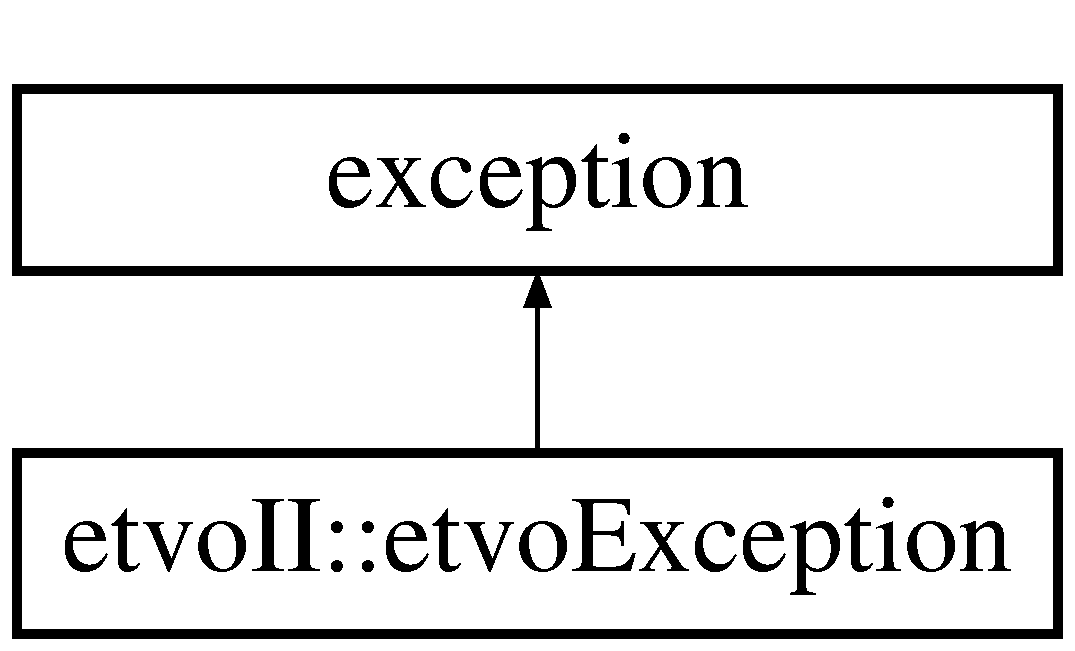
\includegraphics[height=2.000000cm]{classetvo_i_i_1_1etvo_exception}
\end{center}
\end{figure}
\subsection*{Public Member Functions}
\begin{DoxyCompactItemize}
\item 
\mbox{\Hypertarget{classetvo_i_i_1_1etvo_exception_aaf3ee1fbf5a3b7e1ee28c7760d357f33}\label{classetvo_i_i_1_1etvo_exception_aaf3ee1fbf5a3b7e1ee28c7760d357f33}} 
{\bfseries etvo\+Exception} (unsigned num, const std\+::string \&msg)
\item 
\mbox{\Hypertarget{classetvo_i_i_1_1etvo_exception_aa9cffbb354b53bba6faa4d343c621bfa}\label{classetvo_i_i_1_1etvo_exception_aa9cffbb354b53bba6faa4d343c621bfa}} 
unsigned {\bfseries Num} () const
\item 
\mbox{\Hypertarget{classetvo_i_i_1_1etvo_exception_aeed89d0c1ac5f4e39dc2938f8d75e822}\label{classetvo_i_i_1_1etvo_exception_aeed89d0c1ac5f4e39dc2938f8d75e822}} 
std\+::string {\bfseries Message} () const
\end{DoxyCompactItemize}


The documentation for this class was generated from the following files\+:\begin{DoxyCompactItemize}
\item 
etvo/common/etvo\+Exception.\+h\item 
etvo/common/etvo\+Exception.\+cpp\end{DoxyCompactItemize}

\hypertarget{classetvo_i_i_1_1_factory}{}\section{etvo\+II\+:\+:Factory$<$ T $>$ Class Template Reference}
\label{classetvo_i_i_1_1_factory}\index{etvo\+I\+I\+::\+Factory$<$ T $>$@{etvo\+I\+I\+::\+Factory$<$ T $>$}}
\subsection*{Public Member Functions}
\begin{DoxyCompactItemize}
\item 
\mbox{\Hypertarget{classetvo_i_i_1_1_factory_a2361657bfa8883db9c5b2d799afbebec}\label{classetvo_i_i_1_1_factory_a2361657bfa8883db9c5b2d799afbebec}} 
virtual T {\bfseries create} () const =0
\item 
\mbox{\Hypertarget{classetvo_i_i_1_1_factory_acb9d9e4a19ea84a356e5e21f1dbf4cf6}\label{classetvo_i_i_1_1_factory_acb9d9e4a19ea84a356e5e21f1dbf4cf6}} 
virtual std\+::vector$<$ T $>$ {\bfseries createN} (unsigned int n) const
\end{DoxyCompactItemize}


The documentation for this class was generated from the following file\+:\begin{DoxyCompactItemize}
\item 
etvo/factory/factory\+T.\+h\end{DoxyCompactItemize}

\hypertarget{classetvo_i_i_1_1_factory_fper}{}\section{etvo\+II\+:\+:Factory\+Fper Class Reference}
\label{classetvo_i_i_1_1_factory_fper}\index{etvo\+I\+I\+::\+Factory\+Fper@{etvo\+I\+I\+::\+Factory\+Fper}}
Inheritance diagram for etvo\+II\+:\+:Factory\+Fper\+:\begin{figure}[H]
\begin{center}
\leavevmode
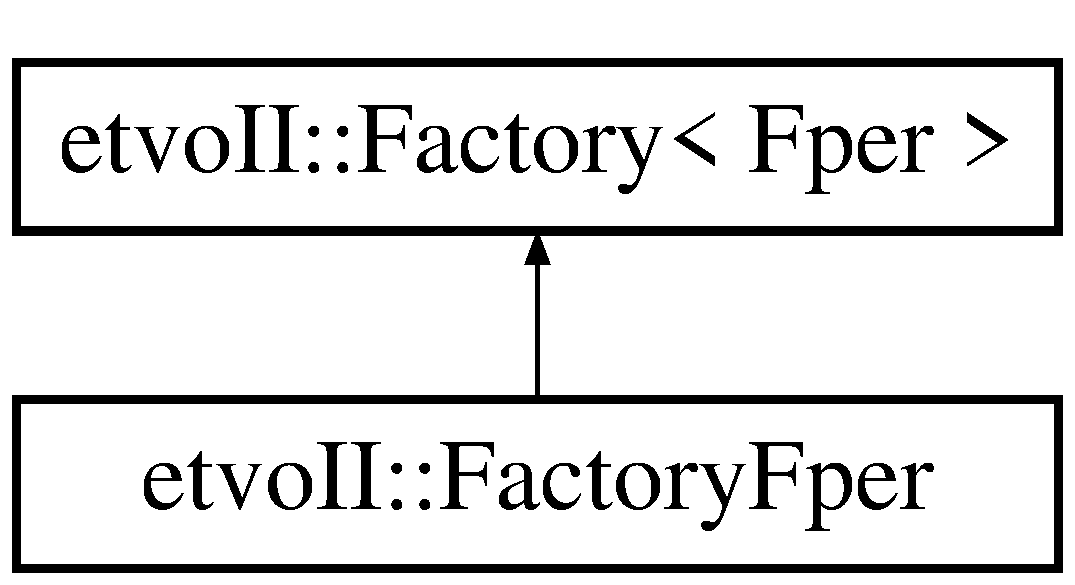
\includegraphics[height=2.000000cm]{classetvo_i_i_1_1_factory_fper}
\end{center}
\end{figure}
\subsection*{Public Member Functions}
\begin{DoxyCompactItemize}
\item 
\mbox{\Hypertarget{classetvo_i_i_1_1_factory_fper_ac61ad54d72b59e5cd1c3056e8240aa6f}\label{classetvo_i_i_1_1_factory_fper_ac61ad54d72b59e5cd1c3056e8240aa6f}} 
{\bfseries Factory\+Fper} (int d, int cod, int Y0, int range\+Y0, bool fixedG=true, bool fixed\+Y0=true)
\item 
\mbox{\Hypertarget{classetvo_i_i_1_1_factory_fper_a00419c2dc7090c04353dedc0a291adc0}\label{classetvo_i_i_1_1_factory_fper_a00419c2dc7090c04353dedc0a291adc0}} 
virtual \mbox{\hyperlink{classetvo_i_i_1_1_fper}{Fper}} {\bfseries create} () const
\end{DoxyCompactItemize}


The documentation for this class was generated from the following files\+:\begin{DoxyCompactItemize}
\item 
etvo/factory/Factory\+Fper.\+h\item 
etvo/factory/Factory\+Fper.\+cpp\end{DoxyCompactItemize}

\hypertarget{classetvo_i_i_1_1_factory_poly}{}\section{etvo\+II\+:\+:Factory\+Poly Class Reference}
\label{classetvo_i_i_1_1_factory_poly}\index{etvo\+I\+I\+::\+Factory\+Poly@{etvo\+I\+I\+::\+Factory\+Poly}}
Inheritance diagram for etvo\+II\+:\+:Factory\+Poly\+:\begin{figure}[H]
\begin{center}
\leavevmode
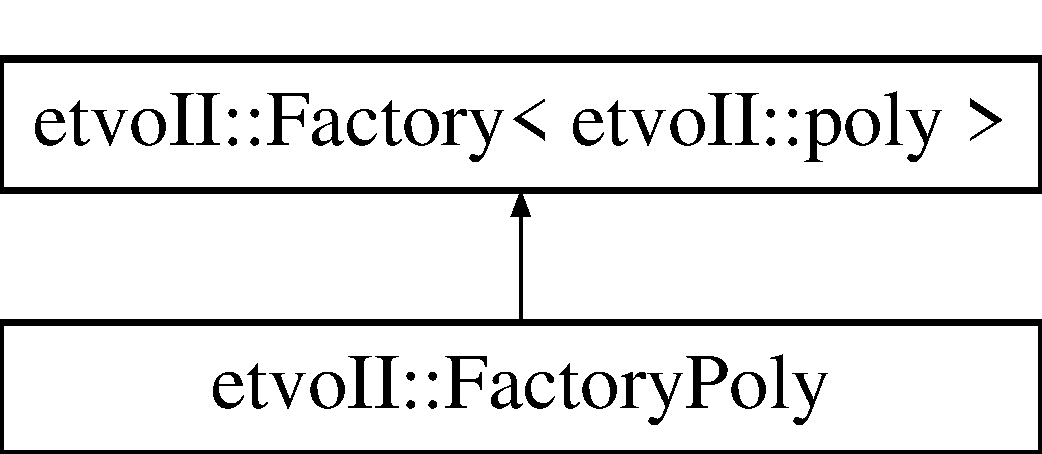
\includegraphics[height=2.000000cm]{classetvo_i_i_1_1_factory_poly}
\end{center}
\end{figure}
\subsection*{Public Member Functions}
\begin{DoxyCompactItemize}
\item 
\mbox{\Hypertarget{classetvo_i_i_1_1_factory_poly_a5d17d3f7ea7986f679a4071df664a23b}\label{classetvo_i_i_1_1_factory_poly_a5d17d3f7ea7986f679a4071df664a23b}} 
{\bfseries Factory\+Poly} (unsigned int nb\+Terms, int gap=5, bool fixed\+Off=true, const \mbox{\hyperlink{classetvo_i_i_1_1gd}{etvo\+I\+I\+::gd}} \&off=\mbox{\hyperlink{classetvo_i_i_1_1gd}{gd}}(0, 0), int range=0)
\item 
\mbox{\Hypertarget{classetvo_i_i_1_1_factory_poly_ac42e8caed1fb4e62384c2fb49e6e7dfa}\label{classetvo_i_i_1_1_factory_poly_ac42e8caed1fb4e62384c2fb49e6e7dfa}} 
virtual \mbox{\hyperlink{classetvo_i_i_1_1poly}{etvo\+I\+I\+::poly}} {\bfseries create} () const
\end{DoxyCompactItemize}


The documentation for this class was generated from the following files\+:\begin{DoxyCompactItemize}
\item 
etvo/factory/Factory\+Poly.\+h\item 
etvo/factory/Factory\+Poly.\+cpp\end{DoxyCompactItemize}

\hypertarget{classetvo_i_i_1_1_factory_poly_ed}{}\section{etvo\+II\+:\+:Factory\+Poly\+Ed Class Reference}
\label{classetvo_i_i_1_1_factory_poly_ed}\index{etvo\+I\+I\+::\+Factory\+Poly\+Ed@{etvo\+I\+I\+::\+Factory\+Poly\+Ed}}
Inheritance diagram for etvo\+II\+:\+:Factory\+Poly\+Ed\+:\begin{figure}[H]
\begin{center}
\leavevmode
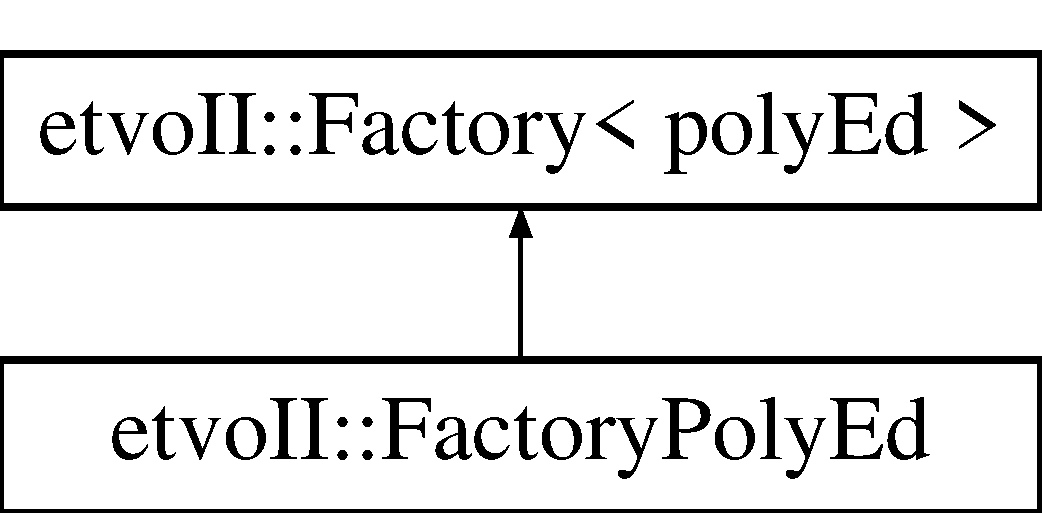
\includegraphics[height=2.000000cm]{classetvo_i_i_1_1_factory_poly_ed}
\end{center}
\end{figure}
\subsection*{Public Member Functions}
\begin{DoxyCompactItemize}
\item 
\mbox{\Hypertarget{classetvo_i_i_1_1_factory_poly_ed_a4d037f3b18493820a5c9abdf6ee4ca64}\label{classetvo_i_i_1_1_factory_poly_ed_a4d037f3b18493820a5c9abdf6ee4ca64}} 
{\bfseries Factory\+Poly\+Ed} (unsigned int nb\+Terms, unsigned int M, unsigned int B, int gap=5, bool fixed\+Gain=true, bool fixed\+Off=true, const \mbox{\hyperlink{classetvo_i_i_1_1gd}{etvo\+I\+I\+::gd}} \&off=\mbox{\hyperlink{classetvo_i_i_1_1gd}{gd}}(0, 0), int range=0)
\item 
\mbox{\Hypertarget{classetvo_i_i_1_1_factory_poly_ed_addf2b16db2accf6e938bf96e18af5c7f}\label{classetvo_i_i_1_1_factory_poly_ed_addf2b16db2accf6e938bf96e18af5c7f}} 
virtual \mbox{\hyperlink{classetvo_i_i_1_1poly_ed}{etvo\+I\+I\+::poly\+Ed}} {\bfseries create} () const
\end{DoxyCompactItemize}


The documentation for this class was generated from the following files\+:\begin{DoxyCompactItemize}
\item 
etvo/factory/Factory\+Poly\+Ed.\+h\item 
etvo/factory/Factory\+Poly\+Ed.\+cpp\end{DoxyCompactItemize}

\hypertarget{classetvo_i_i_1_1_factory_poly_tg}{}\section{etvo\+II\+:\+:Factory\+Poly\+Tg Class Reference}
\label{classetvo_i_i_1_1_factory_poly_tg}\index{etvo\+I\+I\+::\+Factory\+Poly\+Tg@{etvo\+I\+I\+::\+Factory\+Poly\+Tg}}
Inheritance diagram for etvo\+II\+:\+:Factory\+Poly\+Tg\+:\begin{figure}[H]
\begin{center}
\leavevmode
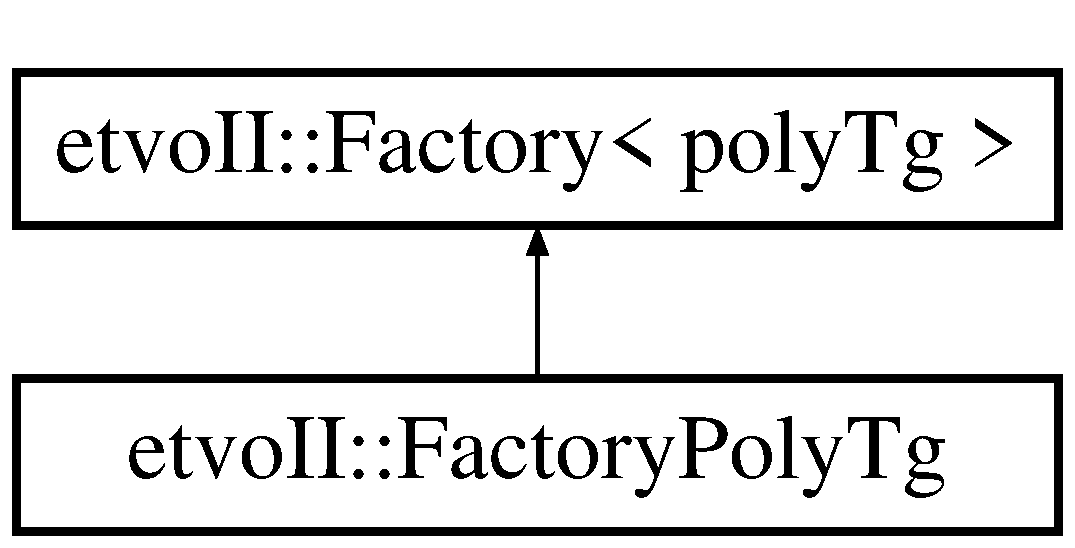
\includegraphics[height=2.000000cm]{classetvo_i_i_1_1_factory_poly_tg}
\end{center}
\end{figure}
\subsection*{Public Member Functions}
\begin{DoxyCompactItemize}
\item 
\mbox{\Hypertarget{classetvo_i_i_1_1_factory_poly_tg_a8d4e35219144179322320573b7de2a41}\label{classetvo_i_i_1_1_factory_poly_tg_a8d4e35219144179322320573b7de2a41}} 
{\bfseries Factory\+Poly\+Tg} (unsigned int nb\+Terms, unsigned int MB, int gap=5, bool fixed\+Gain=true, bool fixed\+Off=true, const \mbox{\hyperlink{classetvo_i_i_1_1gd}{etvo\+I\+I\+::gd}} \&off=\mbox{\hyperlink{classetvo_i_i_1_1gd}{gd}}(0, 0), int range=0)
\item 
\mbox{\Hypertarget{classetvo_i_i_1_1_factory_poly_tg_a2186561e95cb41fa39280b7f93ed28ed}\label{classetvo_i_i_1_1_factory_poly_tg_a2186561e95cb41fa39280b7f93ed28ed}} 
virtual \mbox{\hyperlink{classetvo_i_i_1_1poly_tg}{etvo\+I\+I\+::poly\+Tg}} {\bfseries create} () const
\end{DoxyCompactItemize}


The documentation for this class was generated from the following files\+:\begin{DoxyCompactItemize}
\item 
etvo/factory/Factory\+Poly\+Tg.\+h\item 
etvo/factory/Factory\+Poly\+Tg.\+cpp\end{DoxyCompactItemize}

\hypertarget{classetvo_i_i_1_1_factory_series}{}\section{etvo\+II\+:\+:Factory\+Series Class Reference}
\label{classetvo_i_i_1_1_factory_series}\index{etvo\+I\+I\+::\+Factory\+Series@{etvo\+I\+I\+::\+Factory\+Series}}
Inheritance diagram for etvo\+II\+:\+:Factory\+Series\+:\begin{figure}[H]
\begin{center}
\leavevmode
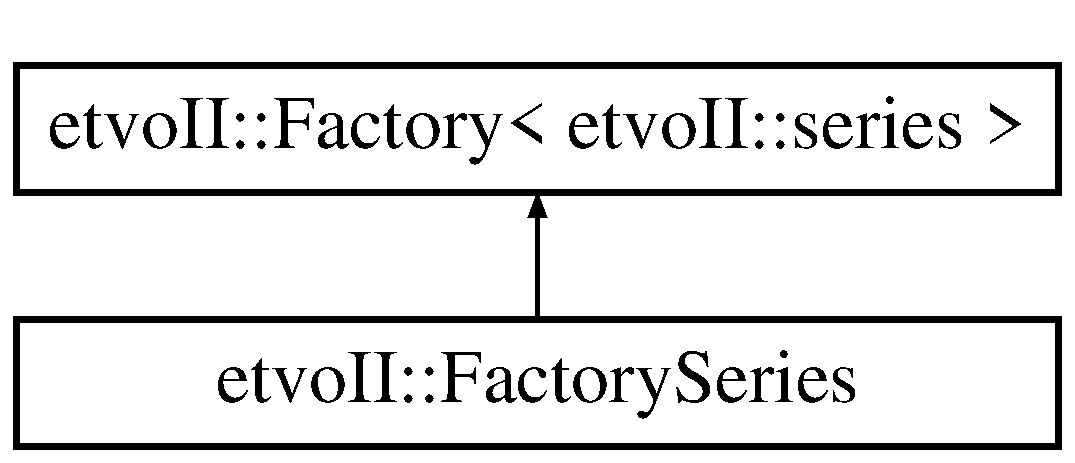
\includegraphics[height=2.000000cm]{classetvo_i_i_1_1_factory_series}
\end{center}
\end{figure}
\subsection*{Public Member Functions}
\begin{DoxyCompactItemize}
\item 
\mbox{\Hypertarget{classetvo_i_i_1_1_factory_series_a7eb04b7a5c5e842777ce132c390f2b56}\label{classetvo_i_i_1_1_factory_series_a7eb04b7a5c5e842777ce132c390f2b56}} 
{\bfseries Factory\+Series} (unsigned int nb\+Terms, const \mbox{\hyperlink{classetvo_i_i_1_1gd}{etvo\+I\+I\+::gd}} \&slopeR, bool fixed\+Slope=true, int gap=5, bool fixed\+Off=true, const \mbox{\hyperlink{classetvo_i_i_1_1gd}{etvo\+I\+I\+::gd}} \&off=\mbox{\hyperlink{classetvo_i_i_1_1gd}{gd}}(0, 0), int range=0)
\item 
\mbox{\Hypertarget{classetvo_i_i_1_1_factory_series_a6fe9c534f741fa3de3a56051f5ca957d}\label{classetvo_i_i_1_1_factory_series_a6fe9c534f741fa3de3a56051f5ca957d}} 
virtual \mbox{\hyperlink{classetvo_i_i_1_1series}{etvo\+I\+I\+::series}} {\bfseries create} () const
\end{DoxyCompactItemize}


The documentation for this class was generated from the following files\+:\begin{DoxyCompactItemize}
\item 
etvo/factory/Factory\+Series.\+h\item 
etvo/factory/Factory\+Series.\+cpp\end{DoxyCompactItemize}

\hypertarget{classetvo_i_i_1_1_factory_series_ed}{}\section{etvo\+II\+:\+:Factory\+Series\+Ed Class Reference}
\label{classetvo_i_i_1_1_factory_series_ed}\index{etvo\+I\+I\+::\+Factory\+Series\+Ed@{etvo\+I\+I\+::\+Factory\+Series\+Ed}}
Inheritance diagram for etvo\+II\+:\+:Factory\+Series\+Ed\+:\begin{figure}[H]
\begin{center}
\leavevmode
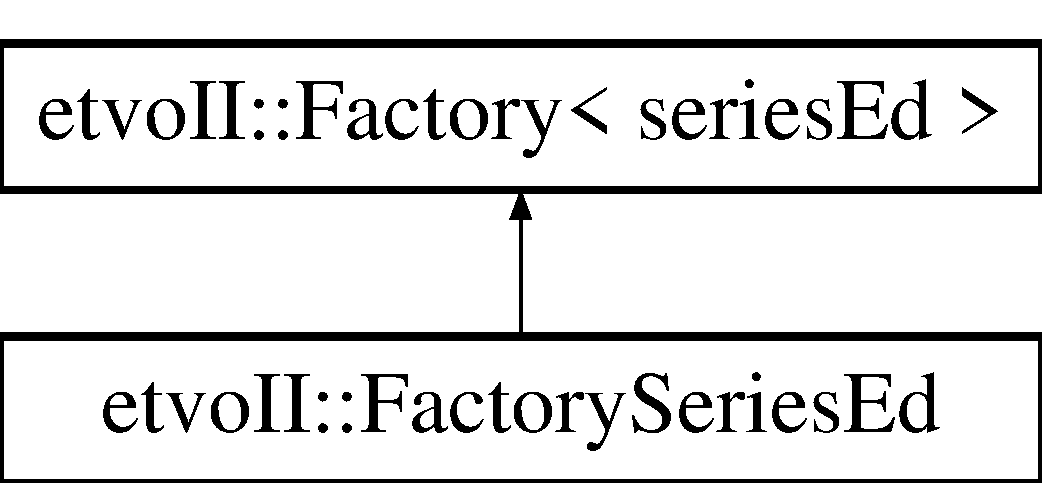
\includegraphics[height=2.000000cm]{classetvo_i_i_1_1_factory_series_ed}
\end{center}
\end{figure}
\subsection*{Public Member Functions}
\begin{DoxyCompactItemize}
\item 
\mbox{\Hypertarget{classetvo_i_i_1_1_factory_series_ed_a7802f76e038a023e3ee9d8be4c9a82b4}\label{classetvo_i_i_1_1_factory_series_ed_a7802f76e038a023e3ee9d8be4c9a82b4}} 
{\bfseries Factory\+Series\+Ed} (unsigned int nb\+Terms, unsigned int M, unsigned int B, const \mbox{\hyperlink{classetvo_i_i_1_1gd}{etvo\+I\+I\+::gd}} \&slopeR, bool fixed\+Slope=true, bool fixed\+Gain=true, bool fixed\+Off=true, const \mbox{\hyperlink{classetvo_i_i_1_1gd}{etvo\+I\+I\+::gd}} \&off=\mbox{\hyperlink{classetvo_i_i_1_1gd}{gd}}(0, 0), int range=0)
\item 
\mbox{\Hypertarget{classetvo_i_i_1_1_factory_series_ed_a45f550b195a9b7dfe9b408e5716ef718}\label{classetvo_i_i_1_1_factory_series_ed_a45f550b195a9b7dfe9b408e5716ef718}} 
virtual \mbox{\hyperlink{classetvo_i_i_1_1series_ed}{etvo\+I\+I\+::series\+Ed}} {\bfseries create} () const
\end{DoxyCompactItemize}


The documentation for this class was generated from the following files\+:\begin{DoxyCompactItemize}
\item 
etvo/factory/Factory\+Series\+Ed.\+h\item 
etvo/factory/Factory\+Series\+Ed.\+cpp\end{DoxyCompactItemize}

\hypertarget{classetvo_i_i_1_1_fmaxp}{}\section{etvo\+II\+:\+:Fmaxp Class Reference}
\label{classetvo_i_i_1_1_fmaxp}\index{etvo\+I\+I\+::\+Fmaxp@{etvo\+I\+I\+::\+Fmaxp}}
Inheritance diagram for etvo\+II\+:\+:Fmaxp\+:\begin{figure}[H]
\begin{center}
\leavevmode
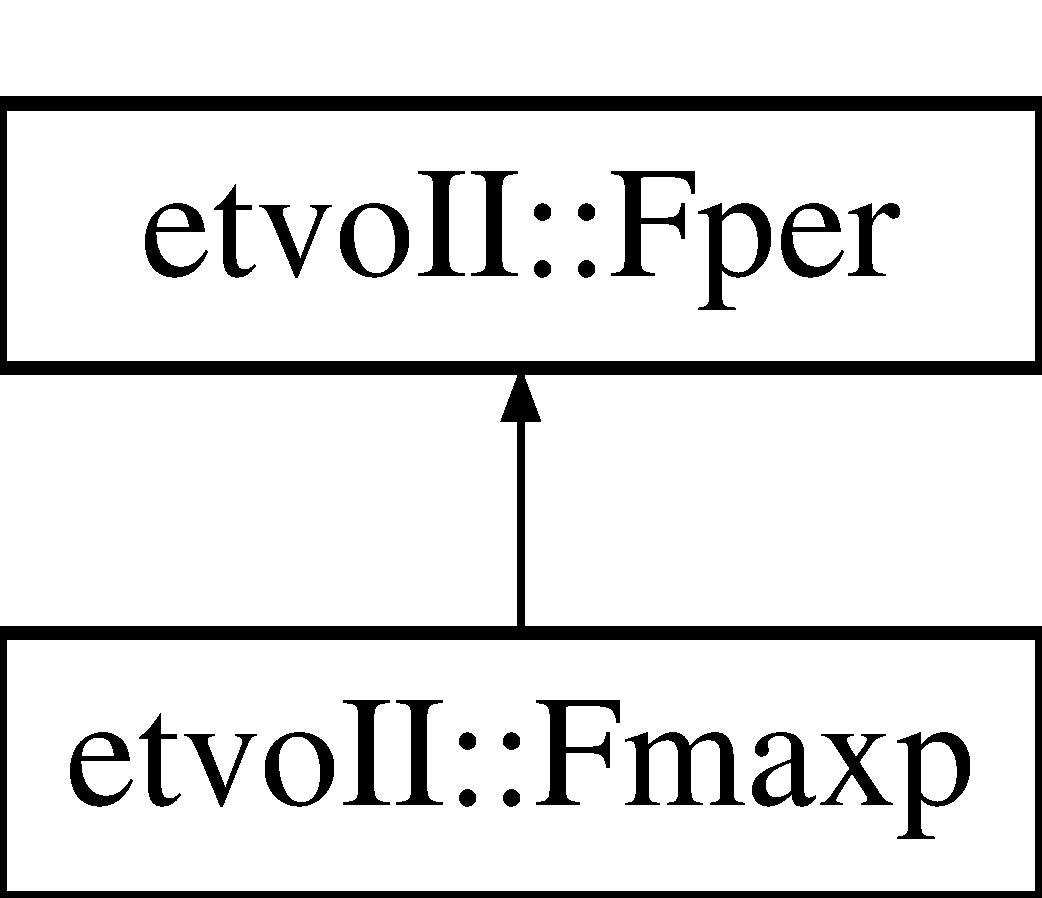
\includegraphics[height=2.000000cm]{classetvo_i_i_1_1_fmaxp}
\end{center}
\end{figure}
\subsection*{Public Member Functions}
\begin{DoxyCompactItemize}
\item 
\mbox{\Hypertarget{classetvo_i_i_1_1_fmaxp_a8a25abfc85dac08a0333d77ea049647e}\label{classetvo_i_i_1_1_fmaxp_a8a25abfc85dac08a0333d77ea049647e}} 
{\bfseries Fmaxp} (int dP, int codP, const std\+::vector$<$ int $>$ \&seq)
\item 
\mbox{\Hypertarget{classetvo_i_i_1_1_fmaxp_ad5a99b9640644bef88f1eaa5777d65ff}\label{classetvo_i_i_1_1_fmaxp_ad5a99b9640644bef88f1eaa5777d65ff}} 
{\bfseries Fmaxp} (const \mbox{\hyperlink{classetvo_i_i_1_1_fper}{Fper}} \&)
\item 
\mbox{\Hypertarget{classetvo_i_i_1_1_fmaxp_ab49bf80d2fa170f7271e50e1e49e6192}\label{classetvo_i_i_1_1_fmaxp_ab49bf80d2fa170f7271e50e1e49e6192}} 
\mbox{\hyperlink{classetvo_i_i_1_1_fmaxp}{Fmaxp}} {\bfseries min} (const \mbox{\hyperlink{classetvo_i_i_1_1_fmaxp}{Fmaxp}} \&) const
\item 
\mbox{\Hypertarget{classetvo_i_i_1_1_fmaxp_a34e208f0e70930980603d8d9c8d73508}\label{classetvo_i_i_1_1_fmaxp_a34e208f0e70930980603d8d9c8d73508}} 
\mbox{\hyperlink{classetvo_i_i_1_1_fmaxp}{Fmaxp}} {\bfseries max} (const \mbox{\hyperlink{classetvo_i_i_1_1_fmaxp}{Fmaxp}} \&) const
\item 
\mbox{\Hypertarget{classetvo_i_i_1_1_fmaxp_a79086bdd6a2464f6765d0f2f1ef20e98}\label{classetvo_i_i_1_1_fmaxp_a79086bdd6a2464f6765d0f2f1ef20e98}} 
\mbox{\hyperlink{classetvo_i_i_1_1_fmaxp}{Fmaxp}} {\bfseries operator+} (const \mbox{\hyperlink{classetvo_i_i_1_1_fmaxp}{Fmaxp}} \&f) const
\item 
\mbox{\Hypertarget{classetvo_i_i_1_1_fmaxp_aae09e9a936f66c77dcdb78753190bcf7}\label{classetvo_i_i_1_1_fmaxp_aae09e9a936f66c77dcdb78753190bcf7}} 
\mbox{\hyperlink{classetvo_i_i_1_1_fmaxp}{Fmaxp}} {\bfseries operator$\ast$} (const \mbox{\hyperlink{classetvo_i_i_1_1_fmaxp}{Fmaxp}} \&f) const
\item 
\mbox{\Hypertarget{classetvo_i_i_1_1_fmaxp_a189a53e2cdddeccf6f4a99158cb063e5}\label{classetvo_i_i_1_1_fmaxp_a189a53e2cdddeccf6f4a99158cb063e5}} 
bool {\bfseries operator==} (const \mbox{\hyperlink{classetvo_i_i_1_1_fmaxp}{Fmaxp}} \&) const
\item 
\mbox{\Hypertarget{classetvo_i_i_1_1_fmaxp_af65b31aa0bfe94b70121c428e51d9ee2}\label{classetvo_i_i_1_1_fmaxp_af65b31aa0bfe94b70121c428e51d9ee2}} 
bool {\bfseries operator!=} (const \mbox{\hyperlink{classetvo_i_i_1_1_fmaxp}{Fmaxp}} \&) const
\item 
\mbox{\Hypertarget{classetvo_i_i_1_1_fmaxp_ac7db4ab710b4cde43f70d6626ea98592}\label{classetvo_i_i_1_1_fmaxp_ac7db4ab710b4cde43f70d6626ea98592}} 
bool {\bfseries operator$<$=} (const \mbox{\hyperlink{classetvo_i_i_1_1_fmaxp}{Fmaxp}} \&) const
\item 
\mbox{\Hypertarget{classetvo_i_i_1_1_fmaxp_a13ec6f5521e1c1ee82458cfa3270ef6c}\label{classetvo_i_i_1_1_fmaxp_a13ec6f5521e1c1ee82458cfa3270ef6c}} 
bool {\bfseries operator$>$=} (const \mbox{\hyperlink{classetvo_i_i_1_1_fmaxp}{Fmaxp}} \&) const
\item 
\mbox{\Hypertarget{classetvo_i_i_1_1_fmaxp_aab37cf27c2048c453c4f00e27750cb78}\label{classetvo_i_i_1_1_fmaxp_aab37cf27c2048c453c4f00e27750cb78}} 
bool {\bfseries operator$<$} (const \mbox{\hyperlink{classetvo_i_i_1_1_fmaxp}{Fmaxp}} \&) const
\item 
\mbox{\Hypertarget{classetvo_i_i_1_1_fmaxp_a14533ec251ebdf8ff52e136a8d7133ca}\label{classetvo_i_i_1_1_fmaxp_a14533ec251ebdf8ff52e136a8d7133ca}} 
bool {\bfseries operator$>$} (const \mbox{\hyperlink{classetvo_i_i_1_1_fmaxp}{Fmaxp}} \&) const
\item 
\mbox{\Hypertarget{classetvo_i_i_1_1_fmaxp_a4064466629ccadd8eccfcb3ea9a64ea3}\label{classetvo_i_i_1_1_fmaxp_a4064466629ccadd8eccfcb3ea9a64ea3}} 
\mbox{\hyperlink{classetvo_i_i_1_1_fmaxp}{Fmaxp}} {\bfseries inf} (const \mbox{\hyperlink{classetvo_i_i_1_1_fmaxp}{Fmaxp}} \&f) const
\item 
\mbox{\hyperlink{classetvo_i_i_1_1_fmaxp}{Fmaxp}} \mbox{\hyperlink{classetvo_i_i_1_1_fmaxp_ad72699ad7193e83e3412cde79c1a461d}{lfrac}} (const \mbox{\hyperlink{classetvo_i_i_1_1_fmaxp}{Fmaxp}} \&a) const
\item 
\mbox{\hyperlink{classetvo_i_i_1_1_fmaxp}{Fmaxp}} \mbox{\hyperlink{classetvo_i_i_1_1_fmaxp_a60837ce28327bcb91be8f5260d90e40c}{rfrac}} (const \mbox{\hyperlink{classetvo_i_i_1_1_fmaxp}{Fmaxp}} \&a) const
\item 
virtual std\+::string \mbox{\hyperlink{classetvo_i_i_1_1_fmaxp_ac9d63f5e1e7eef10af1e3122f5dd4809}{to\+String}} () const
\end{DoxyCompactItemize}
\subsection*{Static Public Member Functions}
\begin{DoxyCompactItemize}
\item 
\mbox{\Hypertarget{classetvo_i_i_1_1_fmaxp_aeeda0aa584bb1d93df2fe63f3634107f}\label{classetvo_i_i_1_1_fmaxp_aeeda0aa584bb1d93df2fe63f3634107f}} 
static \mbox{\hyperlink{classetvo_i_i_1_1_fmaxp}{Fmaxp}} {\bfseries E} ()
\end{DoxyCompactItemize}
\subsection*{Additional Inherited Members}


\subsection{Member Function Documentation}
\mbox{\Hypertarget{classetvo_i_i_1_1_fmaxp_ad72699ad7193e83e3412cde79c1a461d}\label{classetvo_i_i_1_1_fmaxp_ad72699ad7193e83e3412cde79c1a461d}} 
\index{etvo\+I\+I\+::\+Fmaxp@{etvo\+I\+I\+::\+Fmaxp}!lfrac@{lfrac}}
\index{lfrac@{lfrac}!etvo\+I\+I\+::\+Fmaxp@{etvo\+I\+I\+::\+Fmaxp}}
\subsubsection{\texorpdfstring{lfrac()}{lfrac()}}
{\footnotesize\ttfamily \mbox{\hyperlink{classetvo_i_i_1_1_fmaxp}{Fmaxp}} etvo\+I\+I\+::\+Fmaxp\+::lfrac (\begin{DoxyParamCaption}\item[{const \mbox{\hyperlink{classetvo_i_i_1_1_fmaxp}{Fmaxp}} \&}]{a }\end{DoxyParamCaption}) const}

a{\bfseries =} Max \{x $\vert$ a(x)$<$= b\} forall t, x(t)=max\{ tmax $\vert$ f(tmax)$<$=g(t)\} returns a{\bfseries }(b=$\ast$this) ~\newline
~\newline
 result periodicity

I\+N\+IT \mbox{\Hypertarget{classetvo_i_i_1_1_fmaxp_a60837ce28327bcb91be8f5260d90e40c}\label{classetvo_i_i_1_1_fmaxp_a60837ce28327bcb91be8f5260d90e40c}} 
\index{etvo\+I\+I\+::\+Fmaxp@{etvo\+I\+I\+::\+Fmaxp}!rfrac@{rfrac}}
\index{rfrac@{rfrac}!etvo\+I\+I\+::\+Fmaxp@{etvo\+I\+I\+::\+Fmaxp}}
\subsubsection{\texorpdfstring{rfrac()}{rfrac()}}
{\footnotesize\ttfamily \mbox{\hyperlink{classetvo_i_i_1_1_fmaxp}{Fmaxp}} etvo\+I\+I\+::\+Fmaxp\+::rfrac (\begin{DoxyParamCaption}\item[{const \mbox{\hyperlink{classetvo_i_i_1_1_fmaxp}{Fmaxp}} \&}]{a }\end{DoxyParamCaption}) const}

in construction ... returns b/a (b=$\ast$this) ~\newline
~\newline
~\newline
~\newline
 result periodicity

find the least tinit s.\+t. a(tinit)$>$=res\+Dom

a(tinit)$>$=res\+Dom

Fill the begining if not complete \mbox{\Hypertarget{classetvo_i_i_1_1_fmaxp_ac9d63f5e1e7eef10af1e3122f5dd4809}\label{classetvo_i_i_1_1_fmaxp_ac9d63f5e1e7eef10af1e3122f5dd4809}} 
\index{etvo\+I\+I\+::\+Fmaxp@{etvo\+I\+I\+::\+Fmaxp}!to\+String@{to\+String}}
\index{to\+String@{to\+String}!etvo\+I\+I\+::\+Fmaxp@{etvo\+I\+I\+::\+Fmaxp}}
\subsubsection{\texorpdfstring{to\+String()}{toString()}}
{\footnotesize\ttfamily std\+::string etvo\+I\+I\+::\+Fmaxp\+::to\+String (\begin{DoxyParamCaption}{ }\end{DoxyParamCaption}) const\hspace{0.3cm}{\ttfamily [virtual]}}

Returns a string description of a pseudo-\/periodic function Ex\+: \char`\"{}\mbox{[}-\/7 -\/7 -\/3 -\/3 \mbox{]}(4,5)\char`\"{} for a (4,5) pseudo-\/periodic function f(0)=-\/7,f(1)=-\/7,f(2)=-\/3 ... 

Reimplemented from \mbox{\hyperlink{classetvo_i_i_1_1_fper_a53276a36ff7ada879be26655ccff7ed6}{etvo\+I\+I\+::\+Fper}}.



The documentation for this class was generated from the following files\+:\begin{DoxyCompactItemize}
\item 
etvo/\+Fper/Fmaxp.\+h\item 
etvo/\+Fper/Fmaxp.\+cpp\end{DoxyCompactItemize}

\section{etvo\+II\+:\+:Fminp Class Reference}
\label{classetvo_i_i_1_1_fminp}\index{etvo\+I\+I\+::\+Fminp@{etvo\+I\+I\+::\+Fminp}}


Class for pseudo -\/ periodic functions with oplus=min and otimes=composition.  




{\ttfamily \#include $<$Fminp.\+h$>$}



\subsection{Detailed Description}
Class for pseudo -\/ periodic functions with oplus=min and otimes=composition. 

\begin{DoxyAuthor}{Author}
BC L\+A\+R\+IS 
\end{DoxyAuthor}
\begin{DoxyVersion}{Version}
2.\+0 
\end{DoxyVersion}


The documentation for this class was generated from the following file\+:\begin{DoxyCompactItemize}
\item 
C\+:/\+Users/usrlocal/own\+Cloud/\+Dev\+Soft/etvo\+I\+I\+I/etvo19/etvo/\+Fper/\textbf{ Fminp.\+h}\end{DoxyCompactItemize}

\section{etvo\+II\+:\+:Fper Class Reference}
\label{classetvo_i_i_1_1_fper}\index{etvo\+I\+I\+::\+Fper@{etvo\+I\+I\+::\+Fper}}


Base class for pseudo -\/ periodic functions Z-\/$>$Z where f(x + dP) = codP + f(x)  




{\ttfamily \#include $<$Fper.\+h$>$}



\subsection{Detailed Description}
Base class for pseudo -\/ periodic functions Z-\/$>$Z where f(x + dP) = codP + f(x) 

\begin{DoxyAuthor}{Author}
BC L\+A\+R\+IS 
\end{DoxyAuthor}
\begin{DoxyVersion}{Version}
2.\+0 
\end{DoxyVersion}


The documentation for this class was generated from the following file\+:\begin{DoxyCompactItemize}
\item 
C\+:/\+Users/usrlocal/own\+Cloud/\+Dev\+Soft/etvo\+I\+I\+I/etvo19/etvo/\+Fper/\textbf{ Fper.\+h}\end{DoxyCompactItemize}

\hypertarget{classmmgd_1_1gd}{}\section{mmgd\+:\+:gd Class Reference}
\label{classmmgd_1_1gd}\index{mmgd\+::gd@{mmgd\+::gd}}
Inheritance diagram for mmgd\+:\+:gd\+:\begin{figure}[H]
\begin{center}
\leavevmode
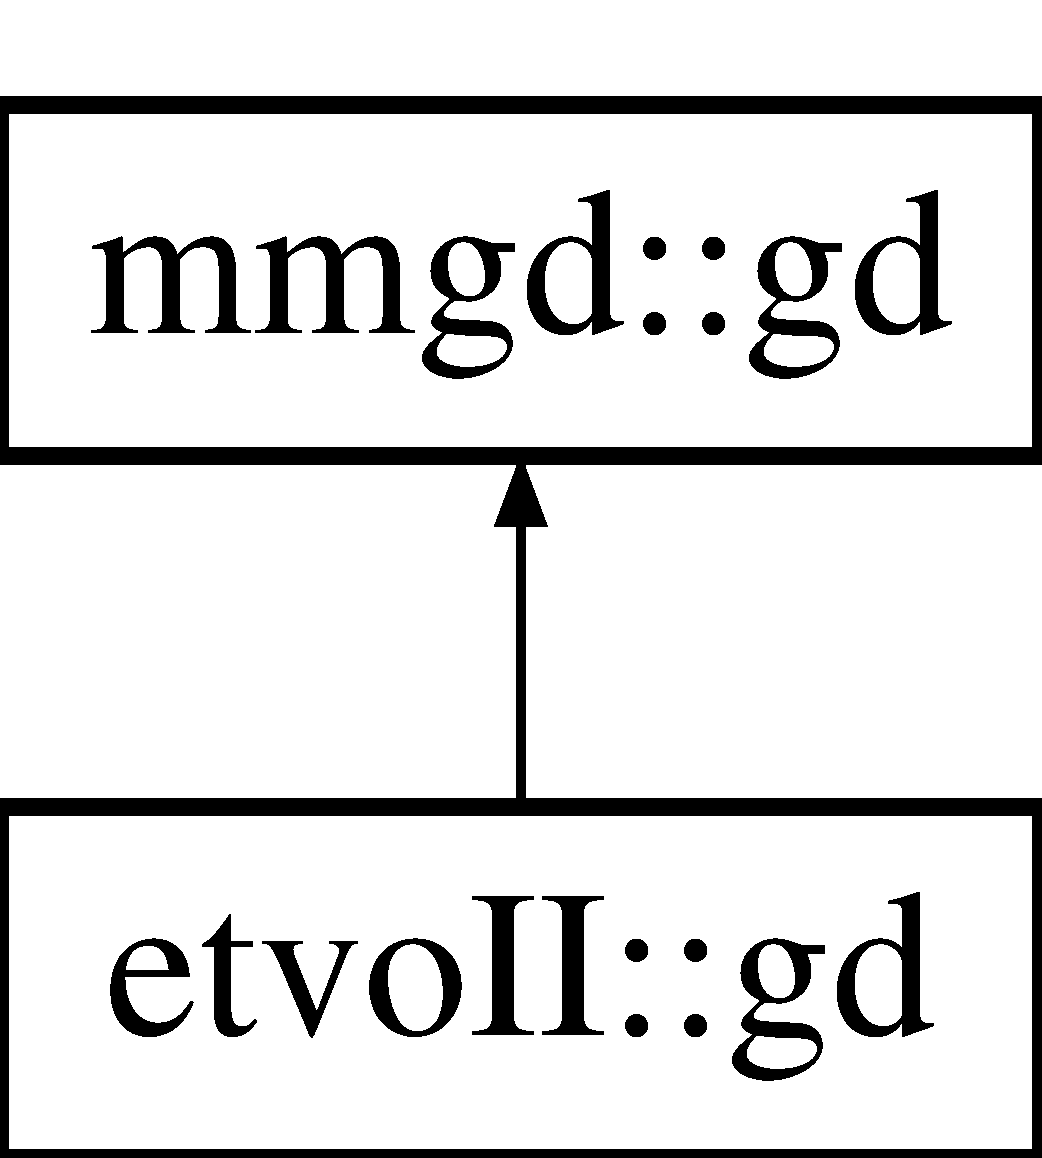
\includegraphics[height=2.000000cm]{classmmgd_1_1gd}
\end{center}
\end{figure}
\subsection*{Public Member Functions}
\begin{DoxyCompactItemize}
\item 
\mbox{\Hypertarget{classmmgd_1_1gd_ac8e74872b52997c0aa6090b82d721e08}\label{classmmgd_1_1gd_ac8e74872b52997c0aa6090b82d721e08}} 
{\bfseries gd} (const \mbox{\hyperlink{classmmgd_1_1gd}{gd}} \&)
\item 
\mbox{\Hypertarget{classmmgd_1_1gd_a512d9003aff50f7b7d2185d7e7272ac6}\label{classmmgd_1_1gd_a512d9003aff50f7b7d2185d7e7272ac6}} 
{\bfseries gd} (long, long)
\item 
\mbox{\Hypertarget{classmmgd_1_1gd_a050613b096bdf3cb95a46d8a207b92cd}\label{classmmgd_1_1gd_a050613b096bdf3cb95a46d8a207b92cd}} 
\mbox{\hyperlink{classmmgd_1_1gd}{gd}} \& {\bfseries operator=} (const \mbox{\hyperlink{classmmgd_1_1gd}{gd}} \&)
\item 
\mbox{\Hypertarget{classmmgd_1_1gd_aceb773d2d343c2c0b9a14f6030d0ac62}\label{classmmgd_1_1gd_aceb773d2d343c2c0b9a14f6030d0ac62}} 
int {\bfseries operator!=} (const \mbox{\hyperlink{classmmgd_1_1gd}{gd}} \&)
\item 
\mbox{\Hypertarget{classmmgd_1_1gd_a4ff3fb6e099001641de565a933d4d898}\label{classmmgd_1_1gd_a4ff3fb6e099001641de565a933d4d898}} 
int {\bfseries operator==} (const \mbox{\hyperlink{classmmgd_1_1gd}{gd}} \&)
\item 
\mbox{\Hypertarget{classmmgd_1_1gd_acfc56cfcff1288f8f4b6120394e7548f}\label{classmmgd_1_1gd_acfc56cfcff1288f8f4b6120394e7548f}} 
int {\bfseries operator$>$=} (const \mbox{\hyperlink{classmmgd_1_1gd}{gd}} \&)
\item 
\mbox{\Hypertarget{classmmgd_1_1gd_a3e38156b0cf3e7cd0a22ba765b874e26}\label{classmmgd_1_1gd_a3e38156b0cf3e7cd0a22ba765b874e26}} 
int {\bfseries operator$<$=} (const \mbox{\hyperlink{classmmgd_1_1gd}{gd}} \&)
\item 
\mbox{\Hypertarget{classmmgd_1_1gd_a89fc335c8bfe23cef630b06e8f1ae507}\label{classmmgd_1_1gd_a89fc335c8bfe23cef630b06e8f1ae507}} 
bool {\bfseries operator$<$} (const \mbox{\hyperlink{classmmgd_1_1gd}{gd}} \&) const
\item 
\mbox{\Hypertarget{classmmgd_1_1gd_a2d04acd086664d7880a2a39ffef3588d}\label{classmmgd_1_1gd_a2d04acd086664d7880a2a39ffef3588d}} 
\mbox{\hyperlink{classmmgd_1_1gd}{gd}} \& {\bfseries init} (long, long)
\item 
\mbox{\Hypertarget{classmmgd_1_1gd_a473a1d68f6362c8b8e7f48aeb38e6461}\label{classmmgd_1_1gd_a473a1d68f6362c8b8e7f48aeb38e6461}} 
\mbox{\hyperlink{classmmgd_1_1gd}{gd}} \& {\bfseries operator()} (long, long)
\item 
\mbox{\Hypertarget{classmmgd_1_1gd_ab452d60ee78b36d09dda2f587f908ce6}\label{classmmgd_1_1gd_ab452d60ee78b36d09dda2f587f908ce6}} 
long {\bfseries getg} (void)
\item 
\mbox{\Hypertarget{classmmgd_1_1gd_af0875481e5b2d5de2f9a2e8a8500aa05}\label{classmmgd_1_1gd_af0875481e5b2d5de2f9a2e8a8500aa05}} 
long {\bfseries getd} (void)
\end{DoxyCompactItemize}
\subsection*{Static Public Attributes}
\begin{DoxyCompactItemize}
\item 
\mbox{\Hypertarget{classmmgd_1_1gd_a406d8038e331c71ec13b5dd00f134207}\label{classmmgd_1_1gd_a406d8038e331c71ec13b5dd00f134207}} 
static \mbox{\hyperlink{classmmgd_1_1gd}{gd}} {\bfseries Top}
\item 
\mbox{\Hypertarget{classmmgd_1_1gd_a066162305c8f563ea3e3bab929c6e94a}\label{classmmgd_1_1gd_a066162305c8f563ea3e3bab929c6e94a}} 
static \mbox{\hyperlink{classmmgd_1_1gd}{gd}} {\bfseries epsilon}
\item 
\mbox{\Hypertarget{classmmgd_1_1gd_afd7496b861bcfa4313382867e16f5ff6}\label{classmmgd_1_1gd_afd7496b861bcfa4313382867e16f5ff6}} 
static \mbox{\hyperlink{classmmgd_1_1gd}{gd}} {\bfseries e}
\end{DoxyCompactItemize}
\subsection*{Protected Member Functions}
\begin{DoxyCompactItemize}
\item 
\mbox{\Hypertarget{classmmgd_1_1gd_a9f0cbddb58f4e9e1c89d03263589af88}\label{classmmgd_1_1gd_a9f0cbddb58f4e9e1c89d03263589af88}} 
void {\bfseries affecte} (long, long)
\end{DoxyCompactItemize}
\subsection*{Protected Attributes}
\begin{DoxyCompactItemize}
\item 
\mbox{\Hypertarget{classmmgd_1_1gd_a4d509ea069575b9c3c4719ebfbfdee59}\label{classmmgd_1_1gd_a4d509ea069575b9c3c4719ebfbfdee59}} 
long {\bfseries g}
\item 
\mbox{\Hypertarget{classmmgd_1_1gd_ab00168800630d031f671ad7057b05aba}\label{classmmgd_1_1gd_ab00168800630d031f671ad7057b05aba}} 
long {\bfseries d}
\end{DoxyCompactItemize}
\subsection*{Friends}
\begin{DoxyCompactItemize}
\item 
\mbox{\Hypertarget{classmmgd_1_1gd_ae6debbf0c1df1dfa98cc657c12c878c1}\label{classmmgd_1_1gd_ae6debbf0c1df1dfa98cc657c12c878c1}} 
std\+::ostream \& {\bfseries operator$<$$<$} (std\+::ostream \&, \mbox{\hyperlink{classmmgd_1_1gd}{gd}} \&)
\item 
\mbox{\Hypertarget{classmmgd_1_1gd_a2652ce1c0563883317a07fd500b1c6ff}\label{classmmgd_1_1gd_a2652ce1c0563883317a07fd500b1c6ff}} 
std\+::fstream \& {\bfseries operator$<$$<$} (std\+::fstream \&, \mbox{\hyperlink{classmmgd_1_1gd}{gd}} \&)
\item 
\mbox{\Hypertarget{classmmgd_1_1gd_a359420ee0032329d8d8273b9fc01d0b7}\label{classmmgd_1_1gd_a359420ee0032329d8d8273b9fc01d0b7}} 
\mbox{\hyperlink{classmmgd_1_1gd}{gd}} {\bfseries inf} (const \mbox{\hyperlink{classmmgd_1_1gd}{gd}} \&gd1, const \mbox{\hyperlink{classmmgd_1_1gd}{gd}} \&gd2)
\item 
\mbox{\Hypertarget{classmmgd_1_1gd_a673acceac37b151854972a1851d1e546}\label{classmmgd_1_1gd_a673acceac37b151854972a1851d1e546}} 
\mbox{\hyperlink{classmmgd_1_1gd}{gd}} {\bfseries otimes} (const \mbox{\hyperlink{classmmgd_1_1gd}{gd}} \&gd1, const \mbox{\hyperlink{classmmgd_1_1gd}{gd}} \&gd2)
\item 
\mbox{\Hypertarget{classmmgd_1_1gd_a3f4a2aa21f57e46b13660bd83cffa8c4}\label{classmmgd_1_1gd_a3f4a2aa21f57e46b13660bd83cffa8c4}} 
\mbox{\hyperlink{classmmgd_1_1gd}{gd}} {\bfseries frac} (const \mbox{\hyperlink{classmmgd_1_1gd}{gd}} \&gd1, const \mbox{\hyperlink{classmmgd_1_1gd}{gd}} \&gd2)
\item 
\mbox{\Hypertarget{classmmgd_1_1gd_a2dd6930af5ca5df0fcb2b684b415c72c}\label{classmmgd_1_1gd_a2dd6930af5ca5df0fcb2b684b415c72c}} 
\mbox{\hyperlink{classmmgd_1_1gd}{gd}} {\bfseries Dualfrac} (const \mbox{\hyperlink{classmmgd_1_1gd}{gd}} \&gd1, const \mbox{\hyperlink{classmmgd_1_1gd}{gd}} \&gd2)
\item 
\mbox{\Hypertarget{classmmgd_1_1gd_a7f189133bc654eb0b9d129cae50b343a}\label{classmmgd_1_1gd_a7f189133bc654eb0b9d129cae50b343a}} 
\mbox{\hyperlink{classmmgd_1_1gd}{gd}} {\bfseries odot} (const \mbox{\hyperlink{classmmgd_1_1gd}{gd}} \&gd1, const \mbox{\hyperlink{classmmgd_1_1gd}{gd}} \&gd2)
\item 
\mbox{\Hypertarget{classmmgd_1_1gd_a4e07c2d7bbd16afdfa616eb51f368b9f}\label{classmmgd_1_1gd_a4e07c2d7bbd16afdfa616eb51f368b9f}} 
\mbox{\hyperlink{classmmgd_1_1gd}{gd}} {\bfseries fracodotsharp} (const \mbox{\hyperlink{classmmgd_1_1gd}{gd}} \&gd1, const \mbox{\hyperlink{classmmgd_1_1gd}{gd}} \&gd2)
\item 
\mbox{\Hypertarget{classmmgd_1_1gd_a204321412b18107581b1d547a931d1ff}\label{classmmgd_1_1gd_a204321412b18107581b1d547a931d1ff}} 
\mbox{\hyperlink{classmmgd_1_1gd}{gd}} {\bfseries fracodotflat} (const \mbox{\hyperlink{classmmgd_1_1gd}{gd}} \&gd1, const \mbox{\hyperlink{classmmgd_1_1gd}{gd}} \&gd2)
\end{DoxyCompactItemize}


The documentation for this class was generated from the following files\+:\begin{DoxyCompactItemize}
\item 
etvo/minmaxgd/gd.\+h\item 
etvo/minmaxgd/gd.\+cpp\end{DoxyCompactItemize}

\hypertarget{classetvo_i_i_1_1gd}{}\section{etvo\+II\+:\+:gd Class Reference}
\label{classetvo_i_i_1_1gd}\index{etvo\+I\+I\+::gd@{etvo\+I\+I\+::gd}}
Inheritance diagram for etvo\+II\+:\+:gd\+:\begin{figure}[H]
\begin{center}
\leavevmode
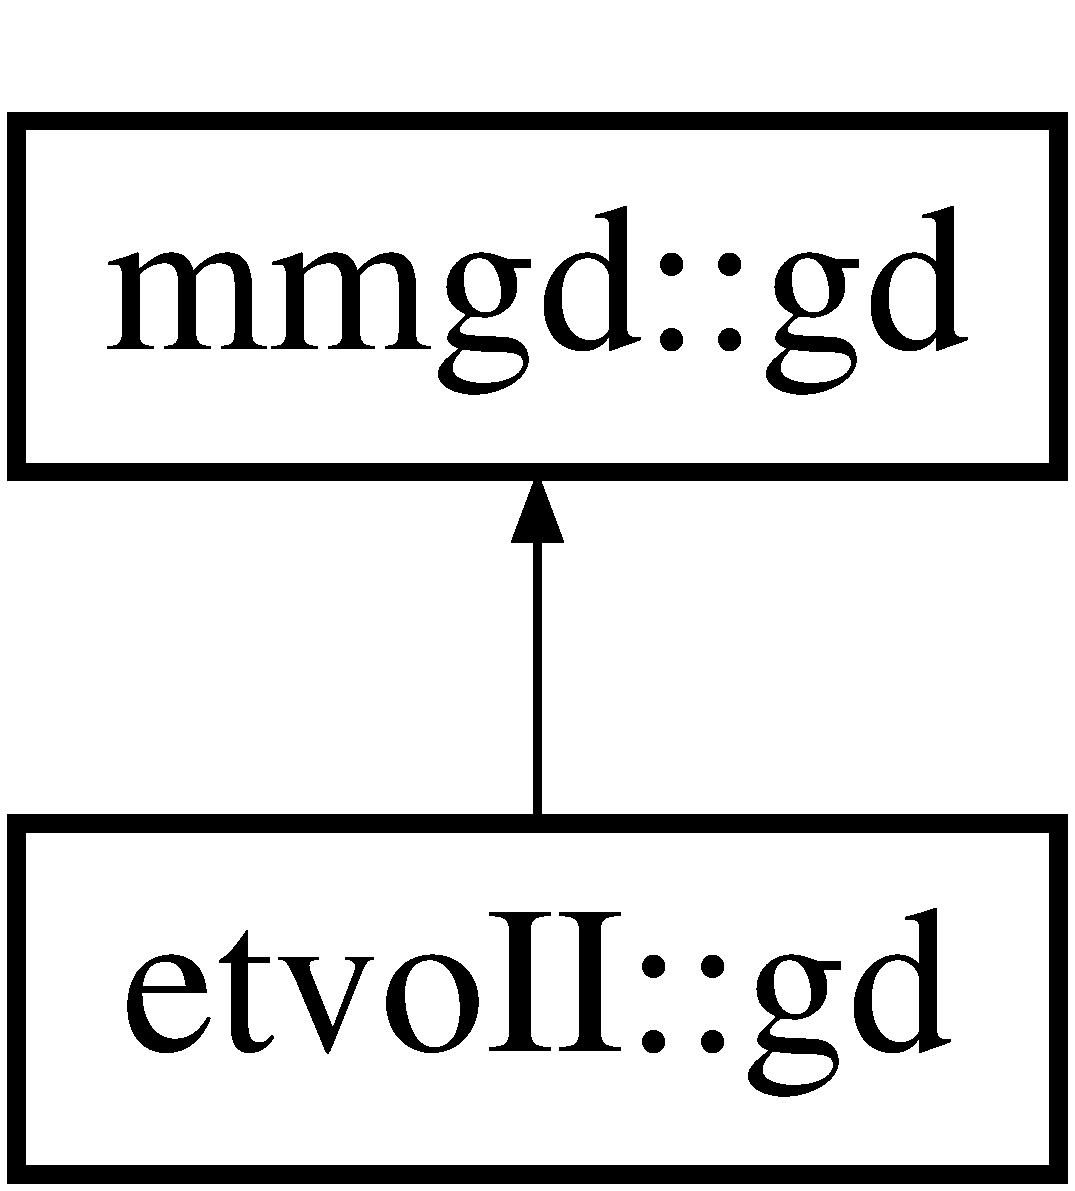
\includegraphics[height=2.000000cm]{classetvo_i_i_1_1gd}
\end{center}
\end{figure}
\subsection*{Public Member Functions}
\begin{DoxyCompactItemize}
\item 
\mbox{\Hypertarget{classetvo_i_i_1_1gd_a907834f286d3b6776280c0daea369825}\label{classetvo_i_i_1_1gd_a907834f286d3b6776280c0daea369825}} 
{\bfseries gd} (long g, long d)
\item 
\mbox{\Hypertarget{classetvo_i_i_1_1gd_a2ba6a8a668b49c1a0d9ec743f6fb26c2}\label{classetvo_i_i_1_1gd_a2ba6a8a668b49c1a0d9ec743f6fb26c2}} 
{\bfseries gd} (const \mbox{\hyperlink{classetvo_i_i_1_1gd}{gd}} \&m)
\item 
\mbox{\Hypertarget{classetvo_i_i_1_1gd_a2af50d7ca46f7909f52e655f4c447a8a}\label{classetvo_i_i_1_1gd_a2af50d7ca46f7909f52e655f4c447a8a}} 
{\bfseries gd} (const \mbox{\hyperlink{classmmgd_1_1gd}{mmgd\+::gd}} \&m)
\item 
\mbox{\Hypertarget{classetvo_i_i_1_1gd_a7d667d50b7d853d4cb6f7479e28e5b91}\label{classetvo_i_i_1_1gd_a7d667d50b7d853d4cb6f7479e28e5b91}} 
\mbox{\hyperlink{classetvo_i_i_1_1gd}{gd}} \& {\bfseries operator=} (const \mbox{\hyperlink{classetvo_i_i_1_1gd}{gd}} \&m)
\item 
\mbox{\Hypertarget{classetvo_i_i_1_1gd_a7590f56c2e1d7e196435b685461a1dfc}\label{classetvo_i_i_1_1gd_a7590f56c2e1d7e196435b685461a1dfc}} 
\mbox{\hyperlink{classetvo_i_i_1_1gd}{gd}} {\bfseries operator$\ast$} (const \mbox{\hyperlink{classetvo_i_i_1_1gd}{gd}} \&m) const
\item 
\mbox{\Hypertarget{classetvo_i_i_1_1gd_a856c302bde775d83ae8960e4fb05f423}\label{classetvo_i_i_1_1gd_a856c302bde775d83ae8960e4fb05f423}} 
long {\bfseries getg} () const
\item 
\mbox{\Hypertarget{classetvo_i_i_1_1gd_a47b2511afe2e3a1bab94a516c5e524dd}\label{classetvo_i_i_1_1gd_a47b2511afe2e3a1bab94a516c5e524dd}} 
long {\bfseries getd} () const
\item 
\mbox{\Hypertarget{classetvo_i_i_1_1gd_a35dfa6812456c575b46682633e4c08f9}\label{classetvo_i_i_1_1gd_a35dfa6812456c575b46682633e4c08f9}} 
bool {\bfseries isE} () const
\item 
\mbox{\Hypertarget{classetvo_i_i_1_1gd_ad736e42b2f93eecfd2178ff489cabb0a}\label{classetvo_i_i_1_1gd_ad736e42b2f93eecfd2178ff489cabb0a}} 
bool {\bfseries operator!=} (const \mbox{\hyperlink{classetvo_i_i_1_1gd}{gd}} \&m) const
\item 
\mbox{\Hypertarget{classetvo_i_i_1_1gd_a8725b56848f17a58154ebaa0b407a4f7}\label{classetvo_i_i_1_1gd_a8725b56848f17a58154ebaa0b407a4f7}} 
bool {\bfseries operator==} (const \mbox{\hyperlink{classetvo_i_i_1_1gd}{gd}} \&) const
\item 
\mbox{\Hypertarget{classetvo_i_i_1_1gd_af6815832a745521df516a446dc46ca55}\label{classetvo_i_i_1_1gd_af6815832a745521df516a446dc46ca55}} 
bool {\bfseries operator$>$=} (const \mbox{\hyperlink{classetvo_i_i_1_1gd}{gd}} \&) const
\item 
\mbox{\Hypertarget{classetvo_i_i_1_1gd_a2b082e42795b21d95b9fb3993e3bce0d}\label{classetvo_i_i_1_1gd_a2b082e42795b21d95b9fb3993e3bce0d}} 
bool {\bfseries operator$<$=} (const \mbox{\hyperlink{classetvo_i_i_1_1gd}{gd}} \&) const
\item 
\mbox{\Hypertarget{classetvo_i_i_1_1gd_abcb521a76cb6f88d843b59794bfc0a08}\label{classetvo_i_i_1_1gd_abcb521a76cb6f88d843b59794bfc0a08}} 
\mbox{\hyperlink{classetvo_i_i_1_1poly}{poly}} {\bfseries operator+} (const \mbox{\hyperlink{classetvo_i_i_1_1gd}{gd}} \&m) const
\item 
\mbox{\Hypertarget{classetvo_i_i_1_1gd_a6177b126400a49eed93dc097e695de78}\label{classetvo_i_i_1_1gd_a6177b126400a49eed93dc097e695de78}} 
\mbox{\hyperlink{classetvo_i_i_1_1poly}{poly}} {\bfseries operator+} (const \mbox{\hyperlink{classetvo_i_i_1_1poly}{poly}} \&p) const
\item 
\mbox{\Hypertarget{classetvo_i_i_1_1gd_a22ada16c77209531f30ba2e9c29299bd}\label{classetvo_i_i_1_1gd_a22ada16c77209531f30ba2e9c29299bd}} 
\mbox{\hyperlink{classetvo_i_i_1_1gd}{gd}} {\bfseries inf} (const \mbox{\hyperlink{classetvo_i_i_1_1gd}{gd}} \&m) const
\item 
\mbox{\Hypertarget{classetvo_i_i_1_1gd_acafc3cdada6c4b78a7f08b988820ca34}\label{classetvo_i_i_1_1gd_acafc3cdada6c4b78a7f08b988820ca34}} 
\mbox{\hyperlink{classetvo_i_i_1_1gd}{gd}} {\bfseries frac} (const \mbox{\hyperlink{classetvo_i_i_1_1gd}{gd}} \&m) const
\item 
\mbox{\Hypertarget{classetvo_i_i_1_1gd_a501d33b5825ea139f9f9271039f408ff}\label{classetvo_i_i_1_1gd_a501d33b5825ea139f9f9271039f408ff}} 
std\+::string {\bfseries To\+String} () const
\end{DoxyCompactItemize}
\subsection*{Static Public Member Functions}
\begin{DoxyCompactItemize}
\item 
\mbox{\Hypertarget{classetvo_i_i_1_1gd_a4a0fc6b9c68ab8e30fc515820fdae3db}\label{classetvo_i_i_1_1gd_a4a0fc6b9c68ab8e30fc515820fdae3db}} 
static \mbox{\hyperlink{classetvo_i_i_1_1gd}{gd}} {\bfseries E} ()
\end{DoxyCompactItemize}
\subsection*{Additional Inherited Members}


The documentation for this class was generated from the following files\+:\begin{DoxyCompactItemize}
\item 
etvo/wrapper\+M\+M\+G\+D/gd\+Wrapper.\+h\item 
etvo/wrapper\+M\+M\+G\+D/gd\+Wrapper.\+cpp\end{DoxyCompactItemize}

\section{global Class Reference}
\label{classglobal}\index{global@{global}}
\subsection*{Static Public Attributes}
\begin{DoxyCompactItemize}
\item 
\mbox{\label{classglobal_a9fe6aeb44df54c3e343f6239074246b3}} 
static int {\bfseries L\+I\+M\+I\+T\+\_\+\+T\+R\+A\+N\+S\+\_\+\+D\+E\+L\+TA} = 2000
\item 
\mbox{\label{classglobal_acc4aeb51e1ad5462dab6fce5ed4ce10f}} 
static unsigned {\bfseries N\+B\+\_\+\+I\+T\+ER} = 20
\item 
\mbox{\label{classglobal_a8153f51df56fd7b014bd0bb6474d2d92}} 
static unsigned {\bfseries N\+B\+\_\+\+L\+O\+O\+PS} = 20
\item 
\mbox{\label{classglobal_a745de8daa78fcc2e02d355bcacdb2047}} 
static unsigned char {\bfseries T\+S\+T\+\_\+\+IS} = 1
\item 
\mbox{\label{classglobal_afdd98731166b06015b81324312a983f6}} 
static unsigned char {\bfseries T\+S\+T\+\_\+\+X\+IS} =2
\item 
\mbox{\label{classglobal_a7aea29eb941a586207d32e4c74c5dbc9}} 
static unsigned char {\bfseries T\+S\+T\+\_\+\+R\+E\+S\+I\+D\+U\+EQ} =4
\item 
\mbox{\label{classglobal_aa6d8b94869d802c205cde70e93f34147}} 
static unsigned char {\bfseries T\+S\+T\+\_\+\+R\+E\+S\+I\+D\+U\+I\+N\+EQ} =8
\item 
\mbox{\label{classglobal_a08bdf876f09fa139ae1ce8e6b8225734}} 
static unsigned char {\bfseries T\+S\+T\+\_\+\+A\+LL} =31
\item 
\mbox{\label{classglobal_a5ece81970bfcede24f93054fe77419c4}} 
static unsigned char {\bfseries T\+S\+T\+\_\+\+K\+L\+E\+E\+NE} = 16
\item 
\mbox{\label{classglobal_a0a9a0abc84481a0cb0ddef8f9288ea69}} 
static long {\bfseries I\+NF} = 2147483647
\item 
\mbox{\label{classglobal_a860fb67122fac26af5eb53e82ea07983}} 
static long {\bfseries \+\_\+\+I\+NF} = -\/2147483647
\end{DoxyCompactItemize}


The documentation for this class was generated from the following files\+:\begin{DoxyCompactItemize}
\item 
F\+:/\+U\+A Box/\+Dev\+Soft/etvo\+I\+I\+I/etvo21/etvo/common/global.\+h\item 
F\+:/\+U\+A Box/\+Dev\+Soft/etvo\+I\+I\+I/etvo21/etvo/common/global.\+cpp\end{DoxyCompactItemize}

\hypertarget{classetvo_i_i_1_1g_ng}{}\section{etvo\+II\+:\+:g\+Ng Class Reference}
\label{classetvo_i_i_1_1g_ng}\index{etvo\+I\+I\+::g\+Ng@{etvo\+I\+I\+::g\+Ng}}


terms like g$^\wedge$nl M\+\_\+m g$^\wedge$nc B\+\_\+b g$^\wedge$nr  




{\ttfamily \#include $<$g\+Ng.\+h$>$}

\subsection*{Public Member Functions}
\begin{DoxyCompactItemize}
\item 
\mbox{\Hypertarget{classetvo_i_i_1_1g_ng_a7b817eff213cb6980af56f6f0398d477}\label{classetvo_i_i_1_1g_ng_a7b817eff213cb6980af56f6f0398d477}} 
\mbox{\hyperlink{classetvo_i_i_1_1g_ng_a7b817eff213cb6980af56f6f0398d477}{g\+Ng}} (int nl, unsigned int m, int nc, unsigned int b, int nr)
\begin{DoxyCompactList}\small\item\em Create term g$^\wedge$nl M\+\_\+m g$^\wedge$nc B\+\_\+b g$^\wedge$nr. \end{DoxyCompactList}\item 
\mbox{\Hypertarget{classetvo_i_i_1_1g_ng_ad3f911b4815d6b2d6cfed7769ceccc15}\label{classetvo_i_i_1_1g_ng_ad3f911b4815d6b2d6cfed7769ceccc15}} 
\mbox{\hyperlink{classetvo_i_i_1_1g_ng_ad3f911b4815d6b2d6cfed7769ceccc15}{g\+Ng}} (int nl, unsigned int m, unsigned int b, int nr)
\begin{DoxyCompactList}\small\item\em Create term g$^\wedge$nl M\+\_\+m g$^\wedge$0 B\+\_\+b g$^\wedge$nr. \end{DoxyCompactList}\item 
\mbox{\Hypertarget{classetvo_i_i_1_1g_ng_aa9a2ce82c40a4567bfca54270fd4a3d8}\label{classetvo_i_i_1_1g_ng_aa9a2ce82c40a4567bfca54270fd4a3d8}} 
\mbox{\hyperlink{classetvo_i_i_1_1g_ng_aa9a2ce82c40a4567bfca54270fd4a3d8}{g\+Ng}} (int nl, unsigned int mb, int nr)
\begin{DoxyCompactList}\small\item\em Create term g$^\wedge$nl M\+\_\+mb g$^\wedge$0 B\+\_\+mb g$^\wedge$nr. \end{DoxyCompactList}\item 
\mbox{\Hypertarget{classetvo_i_i_1_1g_ng_a040cd9c0eab1923496ead6c4545cfba1}\label{classetvo_i_i_1_1g_ng_a040cd9c0eab1923496ead6c4545cfba1}} 
\mbox{\hyperlink{classetvo_i_i_1_1g_ng_a040cd9c0eab1923496ead6c4545cfba1}{g\+Ng}} (int nc)
\begin{DoxyCompactList}\small\item\em g$^\wedge$0 M\+\_\+1 g$^\wedge$nc B\+\_\+1 g$^\wedge$0 = g$^\wedge$nc \end{DoxyCompactList}\item 
\mbox{\Hypertarget{classetvo_i_i_1_1g_ng_aa92563bccdaf0aaeccd21ff9dcedb3a2}\label{classetvo_i_i_1_1g_ng_aa92563bccdaf0aaeccd21ff9dcedb3a2}} 
int \mbox{\hyperlink{classetvo_i_i_1_1g_ng_aa92563bccdaf0aaeccd21ff9dcedb3a2}{get\+Nl}} () const
\begin{DoxyCompactList}\small\item\em getters nl, m, b, br of term g$^\wedge$nl M\+\_\+m B\+\_\+b g$^\wedge$nr \end{DoxyCompactList}\item 
\mbox{\Hypertarget{classetvo_i_i_1_1g_ng_a84fc15c3fcaa968ab41309082516dac3}\label{classetvo_i_i_1_1g_ng_a84fc15c3fcaa968ab41309082516dac3}} 
unsigned int {\bfseries getM} () const
\item 
\mbox{\Hypertarget{classetvo_i_i_1_1g_ng_a7dde7c77f104f5fa1151164d175d1f59}\label{classetvo_i_i_1_1g_ng_a7dde7c77f104f5fa1151164d175d1f59}} 
int {\bfseries get\+Nc} () const
\item 
\mbox{\Hypertarget{classetvo_i_i_1_1g_ng_a742d4c1f56003400ff3570b19b1d7583}\label{classetvo_i_i_1_1g_ng_a742d4c1f56003400ff3570b19b1d7583}} 
unsigned int {\bfseries getB} () const
\item 
\mbox{\Hypertarget{classetvo_i_i_1_1g_ng_aeedcb05be4d265a05d8b8e90fb123d4b}\label{classetvo_i_i_1_1g_ng_aeedcb05be4d265a05d8b8e90fb123d4b}} 
int {\bfseries get\+Nr} () const
\item 
\mbox{\Hypertarget{classetvo_i_i_1_1g_ng_ae119d681053751594bbd46b59ffd1b92}\label{classetvo_i_i_1_1g_ng_ae119d681053751594bbd46b59ffd1b92}} 
bool \mbox{\hyperlink{classetvo_i_i_1_1g_ng_ae119d681053751594bbd46b59ffd1b92}{operator$<$=}} (const \mbox{\hyperlink{classetvo_i_i_1_1g_ng}{g\+Ng}} \&m) const
\begin{DoxyCompactList}\small\item\em comparison of terms (with the same Periodicity) \end{DoxyCompactList}\item 
\mbox{\Hypertarget{classetvo_i_i_1_1g_ng_a37c236ac77b8c91f02cdb3c8060db301}\label{classetvo_i_i_1_1g_ng_a37c236ac77b8c91f02cdb3c8060db301}} 
bool {\bfseries operator$>$=} (const \mbox{\hyperlink{classetvo_i_i_1_1g_ng}{g\+Ng}} \&m) const
\item 
\mbox{\Hypertarget{classetvo_i_i_1_1g_ng_a7393fa830f72d4911ab523c5b21f37c2}\label{classetvo_i_i_1_1g_ng_a7393fa830f72d4911ab523c5b21f37c2}} 
bool {\bfseries operator==} (const \mbox{\hyperlink{classetvo_i_i_1_1g_ng}{g\+Ng}} \&m) const
\item 
\mbox{\Hypertarget{classetvo_i_i_1_1g_ng_a78624342184c361ff14a4eb8215e5832}\label{classetvo_i_i_1_1g_ng_a78624342184c361ff14a4eb8215e5832}} 
void \mbox{\hyperlink{classetvo_i_i_1_1g_ng_a78624342184c361ff14a4eb8215e5832}{canon}} ()
\begin{DoxyCompactList}\small\item\em gives canonical form (depends on set\+Canon\+Form choice) \end{DoxyCompactList}\item 
\mbox{\Hypertarget{classetvo_i_i_1_1g_ng_a0c8273bff466780729524d88173e4973}\label{classetvo_i_i_1_1g_ng_a0c8273bff466780729524d88173e4973}} 
void \mbox{\hyperlink{classetvo_i_i_1_1g_ng_a0c8273bff466780729524d88173e4973}{canonL}} ()
\begin{DoxyCompactList}\small\item\em set Left form \mbox{[}0$<$=nr$<$=b-\/1 and nc=0\mbox{]} \end{DoxyCompactList}\item 
\mbox{\Hypertarget{classetvo_i_i_1_1g_ng_abff475fb0ca90af69ae983560b057e38}\label{classetvo_i_i_1_1g_ng_abff475fb0ca90af69ae983560b057e38}} 
void \mbox{\hyperlink{classetvo_i_i_1_1g_ng_abff475fb0ca90af69ae983560b057e38}{canonC}} ()
\begin{DoxyCompactList}\small\item\em set Central \mbox{[}0$<$=nl$<$=m-\/1 and 0$<$=nr$<$=b-\/1\mbox{]} \end{DoxyCompactList}\item 
\mbox{\Hypertarget{classetvo_i_i_1_1g_ng_a236145cf430e6d4ac456517eebaa5965}\label{classetvo_i_i_1_1g_ng_a236145cf430e6d4ac456517eebaa5965}} 
void \mbox{\hyperlink{classetvo_i_i_1_1g_ng_a236145cf430e6d4ac456517eebaa5965}{canonR}} ()
\begin{DoxyCompactList}\small\item\em set Right form \mbox{[}0$<$=nl$<$=m-\/1 and nc=0\mbox{]} \end{DoxyCompactList}\item 
\mbox{\Hypertarget{classetvo_i_i_1_1g_ng_a9047025599a1b77ecaf1ec848c5d67d3}\label{classetvo_i_i_1_1g_ng_a9047025599a1b77ecaf1ec848c5d67d3}} 
int \mbox{\hyperlink{classetvo_i_i_1_1g_ng_a9047025599a1b77ecaf1ec848c5d67d3}{Fw}} (int ki) const
\begin{DoxyCompactList}\small\item\em value of C/C function Fw(ki) = floor(((nr+ki)/b)+nc)$\ast$m+nl \end{DoxyCompactList}\item 
\mbox{\Hypertarget{classetvo_i_i_1_1g_ng_a86b5837b0df28b1c3dfb84aeff8a1d73}\label{classetvo_i_i_1_1g_ng_a86b5837b0df28b1c3dfb84aeff8a1d73}} 
\mbox{\hyperlink{classetvo_i_i_1_1_fminp}{Fminp}} \mbox{\hyperlink{classetvo_i_i_1_1g_ng_a86b5837b0df28b1c3dfb84aeff8a1d73}{get\+Fw}} () const
\begin{DoxyCompactList}\small\item\em returns function Fw \end{DoxyCompactList}\item 
\mbox{\Hypertarget{classetvo_i_i_1_1g_ng_ac654c7ec491ab5a184137e01a202ef2e}\label{classetvo_i_i_1_1g_ng_ac654c7ec491ab5a184137e01a202ef2e}} 
\mbox{\hyperlink{classetvo_i_i_1_1_e__op}{E\+\_\+op}} \mbox{\hyperlink{classetvo_i_i_1_1g_ng_ac654c7ec491ab5a184137e01a202ef2e}{extend\+By}} (unsigned mul) const
\begin{DoxyCompactList}\small\item\em Extension of g$^\wedge$nl M\+\_\+m B\+\_\+b g$^\wedge$nr -\/$>$ S\+U\+M\+\_\+i g$^\wedge$(nl+i$\ast$ M\+\_\+(mul$\ast$m) B\+\_\+(mul$\ast$\+\_\+b) g$^\wedge$(mul-\/1) .... \end{DoxyCompactList}\item 
\mbox{\Hypertarget{classetvo_i_i_1_1g_ng_aaa615f59e4855b8977cc8f0ec2ed90f2}\label{classetvo_i_i_1_1g_ng_aaa615f59e4855b8977cc8f0ec2ed90f2}} 
std\+::pair$<$ unsigned, unsigned $>$ \mbox{\hyperlink{classetvo_i_i_1_1g_ng_aaa615f59e4855b8977cc8f0ec2ed90f2}{get\+Periodicity}} () const
\begin{DoxyCompactList}\small\item\em periodicity as a pair $<$\+\_\+b,\+\_\+m$>$ \end{DoxyCompactList}\item 
\mbox{\Hypertarget{classetvo_i_i_1_1g_ng_a78675574e1c1077aa66bef9dfbc2056c}\label{classetvo_i_i_1_1g_ng_a78675574e1c1077aa66bef9dfbc2056c}} 
std\+::string \mbox{\hyperlink{classetvo_i_i_1_1g_ng_a78675574e1c1077aa66bef9dfbc2056c}{to\+String}} (unsigned n\+Ver=0) const
\begin{DoxyCompactList}\small\item\em gain rational(m/b) \end{DoxyCompactList}\end{DoxyCompactItemize}
\subsection*{Static Public Member Functions}
\begin{DoxyCompactItemize}
\item 
\mbox{\Hypertarget{classetvo_i_i_1_1g_ng_a6ceb1e64283a16aeec64dcc3a40ce4d9}\label{classetvo_i_i_1_1g_ng_a6ceb1e64283a16aeec64dcc3a40ce4d9}} 
static void {\bfseries set\+Canon\+Form} (unsigned val=0)
\end{DoxyCompactItemize}
\subsection*{Protected Attributes}
\begin{DoxyCompactItemize}
\item 
\mbox{\Hypertarget{classetvo_i_i_1_1g_ng_a9cb6c20901b91d34dd17157668ccd199}\label{classetvo_i_i_1_1g_ng_a9cb6c20901b91d34dd17157668ccd199}} 
int \mbox{\hyperlink{classetvo_i_i_1_1g_ng_a9cb6c20901b91d34dd17157668ccd199}{\+\_\+nl}}
\begin{DoxyCompactList}\small\item\em nl,m,b,nr \end{DoxyCompactList}\item 
\mbox{\Hypertarget{classetvo_i_i_1_1g_ng_aa167ce6f4030dc5fae3e10750668d970}\label{classetvo_i_i_1_1g_ng_aa167ce6f4030dc5fae3e10750668d970}} 
unsigned int {\bfseries \+\_\+m}
\item 
\mbox{\Hypertarget{classetvo_i_i_1_1g_ng_a4b856ea7fb171e3cdb619631dd78cfdd}\label{classetvo_i_i_1_1g_ng_a4b856ea7fb171e3cdb619631dd78cfdd}} 
int {\bfseries \+\_\+nc}
\item 
\mbox{\Hypertarget{classetvo_i_i_1_1g_ng_acfd602904616c0b6e5a51b35113fd9a3}\label{classetvo_i_i_1_1g_ng_acfd602904616c0b6e5a51b35113fd9a3}} 
unsigned int {\bfseries \+\_\+b}
\item 
\mbox{\Hypertarget{classetvo_i_i_1_1g_ng_ae0b4168e235fae57436f78e7c3362100}\label{classetvo_i_i_1_1g_ng_ae0b4168e235fae57436f78e7c3362100}} 
int {\bfseries \+\_\+nr}
\end{DoxyCompactItemize}
\subsection*{Static Protected Attributes}
\begin{DoxyCompactItemize}
\item 
static unsigned \mbox{\hyperlink{classetvo_i_i_1_1g_ng_a788cd29adc53a556f5070d76cfbd80b2}{\+\_\+canon}} =0
\begin{DoxyCompactList}\small\item\em set canonical form of \mbox{\hyperlink{classetvo_i_i_1_1g_ng}{g\+Ng}} (default left form) \end{DoxyCompactList}\end{DoxyCompactItemize}


\subsection{Detailed Description}
terms like g$^\wedge$nl M\+\_\+m g$^\wedge$nc B\+\_\+b g$^\wedge$nr 

\subsection{Member Data Documentation}
\mbox{\Hypertarget{classetvo_i_i_1_1g_ng_a788cd29adc53a556f5070d76cfbd80b2}\label{classetvo_i_i_1_1g_ng_a788cd29adc53a556f5070d76cfbd80b2}} 
\index{etvo\+I\+I\+::g\+Ng@{etvo\+I\+I\+::g\+Ng}!\+\_\+canon@{\+\_\+canon}}
\index{\+\_\+canon@{\+\_\+canon}!etvo\+I\+I\+::g\+Ng@{etvo\+I\+I\+::g\+Ng}}
\subsubsection{\texorpdfstring{\+\_\+canon}{\_canon}}
{\footnotesize\ttfamily unsigned etvo\+I\+I\+::g\+Ng\+::\+\_\+canon =0\hspace{0.3cm}{\ttfamily [static]}, {\ttfamily [protected]}}



set canonical form of \mbox{\hyperlink{classetvo_i_i_1_1g_ng}{g\+Ng}} (default left form) 

set the default form as Central Form 

The documentation for this class was generated from the following files\+:\begin{DoxyCompactItemize}
\item 
etvo/etop/g\+Ng.\+h\item 
etvo/etop/g\+Ng.\+cpp\end{DoxyCompactItemize}

\section{etvo\+II\+:\+:I\+Sterm Class Reference}
\label{classetvo_i_i_1_1_i_sterm}\index{etvo\+I\+I\+::\+I\+Sterm@{etvo\+I\+I\+::\+I\+Sterm}}


Abstract base class to handle Idempotent Semiring terms.  




{\ttfamily \#include $<$I\+Sterm.\+h$>$}



\subsection{Detailed Description}
Abstract base class to handle Idempotent Semiring terms. 

Attribute \+\_\+eps\+N\+Top describes epsilon (-\/1) Top(+1) and Not extrem (0)

\begin{DoxyAuthor}{Author}
BC L\+A\+R\+IS 
\end{DoxyAuthor}
\begin{DoxyVersion}{Version}
2.\+0 
\end{DoxyVersion}


The documentation for this class was generated from the following file\+:\begin{DoxyCompactItemize}
\item 
C\+:/\+Users/usrlocal/own\+Cloud/\+Dev\+Soft/etvo\+I\+I\+I/etvo19/etvo/common/\textbf{ I\+Sterm.\+h}\end{DoxyCompactItemize}

\hypertarget{classetvo_i_i_1_1matrix}{}\section{etvo\+II\+:\+:matrix$<$ T $>$ Class Template Reference}
\label{classetvo_i_i_1_1matrix}\index{etvo\+I\+I\+::matrix$<$ T $>$@{etvo\+I\+I\+::matrix$<$ T $>$}}
\subsection*{Public Member Functions}
\begin{DoxyCompactItemize}
\item 
\mbox{\Hypertarget{classetvo_i_i_1_1matrix_afd7d69ed3bbae7d524e850ac13ec4ac8}\label{classetvo_i_i_1_1matrix_afd7d69ed3bbae7d524e850ac13ec4ac8}} 
{\bfseries operator T} ()
\item 
\mbox{\Hypertarget{classetvo_i_i_1_1matrix_a94e3340d596dccb804be55a791e7c40c}\label{classetvo_i_i_1_1matrix_a94e3340d596dccb804be55a791e7c40c}} 
{\bfseries matrix} (unsigned li=1, unsigned co=1)
\item 
\mbox{\Hypertarget{classetvo_i_i_1_1matrix_a1c6e2bdb5f36125ace183ef2c0b8384a}\label{classetvo_i_i_1_1matrix_a1c6e2bdb5f36125ace183ef2c0b8384a}} 
T \& {\bfseries operator()} (unsigned li, unsigned co)
\item 
\mbox{\Hypertarget{classetvo_i_i_1_1matrix_aabea634af0454bcf58867ff155a7f764}\label{classetvo_i_i_1_1matrix_aabea634af0454bcf58867ff155a7f764}} 
T {\bfseries operator()} (unsigned li, unsigned co) const
\item 
\mbox{\Hypertarget{classetvo_i_i_1_1matrix_a6d14e19a2c42197b91aff8ba6490676c}\label{classetvo_i_i_1_1matrix_a6d14e19a2c42197b91aff8ba6490676c}} 
\mbox{\hyperlink{classetvo_i_i_1_1matrix}{matrix}}$<$ T $>$ {\bfseries operator+} (const \mbox{\hyperlink{classetvo_i_i_1_1matrix}{matrix}}$<$ T $>$ \&mat) const
\item 
\mbox{\Hypertarget{classetvo_i_i_1_1matrix_a1a3e5c841be234955c330a84fa289ec7}\label{classetvo_i_i_1_1matrix_a1a3e5c841be234955c330a84fa289ec7}} 
\mbox{\hyperlink{classetvo_i_i_1_1matrix}{matrix}}$<$ T $>$ {\bfseries operator$\ast$} (const \mbox{\hyperlink{classetvo_i_i_1_1matrix}{matrix}}$<$ T $>$ \&mat) const
\item 
\mbox{\Hypertarget{classetvo_i_i_1_1matrix_a76a39a436002a07fb8124501029a5e9d}\label{classetvo_i_i_1_1matrix_a76a39a436002a07fb8124501029a5e9d}} 
\mbox{\hyperlink{classetvo_i_i_1_1matrix}{matrix}}$<$ T $>$ {\bfseries lfrac} (const \mbox{\hyperlink{classetvo_i_i_1_1matrix}{matrix}}$<$ T $>$ \&mat) const
\item 
\mbox{\Hypertarget{classetvo_i_i_1_1matrix_a837e32704f2ffd4222ade7e3bf511613}\label{classetvo_i_i_1_1matrix_a837e32704f2ffd4222ade7e3bf511613}} 
\mbox{\hyperlink{classetvo_i_i_1_1matrix}{matrix}}$<$ T $>$ {\bfseries rfrac} (const \mbox{\hyperlink{classetvo_i_i_1_1matrix}{matrix}}$<$ T $>$ \&mat) const
\item 
\mbox{\Hypertarget{classetvo_i_i_1_1matrix_ae8113541eac59b1d4e306d7e28ce9025}\label{classetvo_i_i_1_1matrix_ae8113541eac59b1d4e306d7e28ce9025}} 
\mbox{\hyperlink{classetvo_i_i_1_1matrix}{matrix}}$<$ T $>$ {\bfseries inf} (const \mbox{\hyperlink{classetvo_i_i_1_1matrix}{matrix}}$<$ T $>$ \&mat) const
\item 
\mbox{\Hypertarget{classetvo_i_i_1_1matrix_a398e9ebe11c9a3656a0dea8f2f558dc8}\label{classetvo_i_i_1_1matrix_a398e9ebe11c9a3656a0dea8f2f558dc8}} 
\mbox{\hyperlink{classetvo_i_i_1_1matrix}{matrix}}$<$ T $>$ {\bfseries star} () const
\item 
\mbox{\Hypertarget{classetvo_i_i_1_1matrix_a2aee163327f9b8df41cce9a227d13710}\label{classetvo_i_i_1_1matrix_a2aee163327f9b8df41cce9a227d13710}} 
unsigned int {\bfseries Get\+Row} () const
\item 
\mbox{\Hypertarget{classetvo_i_i_1_1matrix_a4993db01a58342feec5578ffa4b41e26}\label{classetvo_i_i_1_1matrix_a4993db01a58342feec5578ffa4b41e26}} 
unsigned int {\bfseries Get\+Column} () const
\item 
\mbox{\Hypertarget{classetvo_i_i_1_1matrix_ab294d43a3e8f7bb49202516d53b65775}\label{classetvo_i_i_1_1matrix_ab294d43a3e8f7bb49202516d53b65775}} 
bool {\bfseries operator==} (const \mbox{\hyperlink{classetvo_i_i_1_1matrix}{matrix}}$<$ T $>$ \&m) const
\end{DoxyCompactItemize}


The documentation for this class was generated from the following file\+:\begin{DoxyCompactItemize}
\item 
etvo/wrapper\+M\+M\+G\+D/matrix\+Wrapper.\+h\end{DoxyCompactItemize}

\section{mmgd\+:\+:mem\+\_\+limite Class Reference}
\label{classmmgd_1_1mem__limite}\index{mmgd\+::mem\+\_\+limite@{mmgd\+::mem\+\_\+limite}}
\subsection*{Public Member Functions}
\begin{DoxyCompactItemize}
\item 
\mbox{\label{classmmgd_1_1mem__limite_ab00a238d0429a5bf079c4534db8b912c}} 
{\bfseries mem\+\_\+limite} (int i)
\end{DoxyCompactItemize}
\subsection*{Public Attributes}
\begin{DoxyCompactItemize}
\item 
\mbox{\label{classmmgd_1_1mem__limite_ade5cb5c82021ac0faaf831ab83ece8ae}} 
int {\bfseries memoire}
\end{DoxyCompactItemize}


The documentation for this class was generated from the following file\+:\begin{DoxyCompactItemize}
\item 
F\+:/\+U\+A Box/\+Dev\+Soft/etvo\+I\+I\+I/etvo21/etvo/libminmaxgd/include/gd.\+h\end{DoxyCompactItemize}

\hypertarget{classetvo_i_i_1_1parser}{}\section{etvo\+II\+:\+:parser Class Reference}
\label{classetvo_i_i_1_1parser}\index{etvo\+I\+I\+::parser@{etvo\+I\+I\+::parser}}
\subsection*{Static Public Member Functions}
\begin{DoxyCompactItemize}
\item 
\mbox{\Hypertarget{classetvo_i_i_1_1parser_aaf779f48960c18a9021b6270752f44ca}\label{classetvo_i_i_1_1parser_aaf779f48960c18a9021b6270752f44ca}} 
static \mbox{\hyperlink{classetvo_i_i_1_1poly_ed}{poly\+Ed}} {\bfseries parse\+Poly\+Ed} (const std\+::string \&s)
\item 
\mbox{\Hypertarget{classetvo_i_i_1_1parser_aba1401a254d4227d4bc6f236efc2f4c3}\label{classetvo_i_i_1_1parser_aba1401a254d4227d4bc6f236efc2f4c3}} 
static \mbox{\hyperlink{classetvo_i_i_1_1series_ed}{series\+Ed}} {\bfseries parse\+Series\+Ed} (const std\+::string \&s)
\item 
\mbox{\Hypertarget{classetvo_i_i_1_1parser_acdcc3451e69e50b0e3f8c24cac299bf8}\label{classetvo_i_i_1_1parser_acdcc3451e69e50b0e3f8c24cac299bf8}} 
static \mbox{\hyperlink{classetvo_i_i_1_1poly_tg}{poly\+Tg}} {\bfseries parse\+Poly\+Tg} (const std\+::string \&s)
\item 
\mbox{\Hypertarget{classetvo_i_i_1_1parser_a61226859a639ceaa441064f321766527}\label{classetvo_i_i_1_1parser_a61226859a639ceaa441064f321766527}} 
static \mbox{\hyperlink{classetvo_i_i_1_1poly}{poly}} {\bfseries parse\+Poly} (const std\+::string \&str)
\item 
\mbox{\Hypertarget{classetvo_i_i_1_1parser_ae871e7ac21dfcca6e707729722c5818d}\label{classetvo_i_i_1_1parser_ae871e7ac21dfcca6e707729722c5818d}} 
static void {\bfseries run\+Calculator\+Etvo} ()
\end{DoxyCompactItemize}


The documentation for this class was generated from the following files\+:\begin{DoxyCompactItemize}
\item 
etvo/parsers/parser.\+h\item 
etvo/parsers/calculator.\+cpp\item 
etvo/parsers/parser.\+cpp\item 
etvo/parsers/parser\+Series\+Ed.\+cpp\end{DoxyCompactItemize}

\section{Pov\+Ray\+:\+:Pov\+Ray2\+:\+:Point Class Reference}
\label{class_pov_ray_1_1_pov_ray2_1_1_point}\index{Pov\+Ray\+::\+Pov\+Ray2\+::\+Point@{Pov\+Ray\+::\+Pov\+Ray2\+::\+Point}}
\subsection*{Public Member Functions}
\begin{DoxyCompactItemize}
\item 
\mbox{\label{class_pov_ray_1_1_pov_ray2_1_1_point_aaad775e15b0968f3a4b8991aa1c67c77}} 
{\bfseries Point} (float X=0, float Y=0, float Z=0)
\item 
\mbox{\label{class_pov_ray_1_1_pov_ray2_1_1_point_aab7b20ba9e713159f1f54f0685a64a42}} 
std\+::string {\bfseries To\+String} ()
\end{DoxyCompactItemize}
\subsection*{Public Attributes}
\begin{DoxyCompactItemize}
\item 
\mbox{\label{class_pov_ray_1_1_pov_ray2_1_1_point_ae263d2db95131761a3210715e5a2c4f5}} 
float {\bfseries x}
\item 
\mbox{\label{class_pov_ray_1_1_pov_ray2_1_1_point_affc0692adeada35a2c4578bad78ae8e1}} 
float {\bfseries y}
\item 
\mbox{\label{class_pov_ray_1_1_pov_ray2_1_1_point_ad5362439150ce1146f38a0bd847a3584}} 
float {\bfseries z}
\end{DoxyCompactItemize}


The documentation for this class was generated from the following file\+:\begin{DoxyCompactItemize}
\item 
F\+:/\+U\+A Box/\+Dev\+Soft/etvo\+I\+I\+I/etvo21/etvo/grafic/Pov\+Ray2.\+h\end{DoxyCompactItemize}

\hypertarget{classmmgd_1_1poly}{}\section{mmgd\+:\+:poly Class Reference}
\label{classmmgd_1_1poly}\index{mmgd\+::poly@{mmgd\+::poly}}
Inheritance diagram for mmgd\+:\+:poly\+:\begin{figure}[H]
\begin{center}
\leavevmode
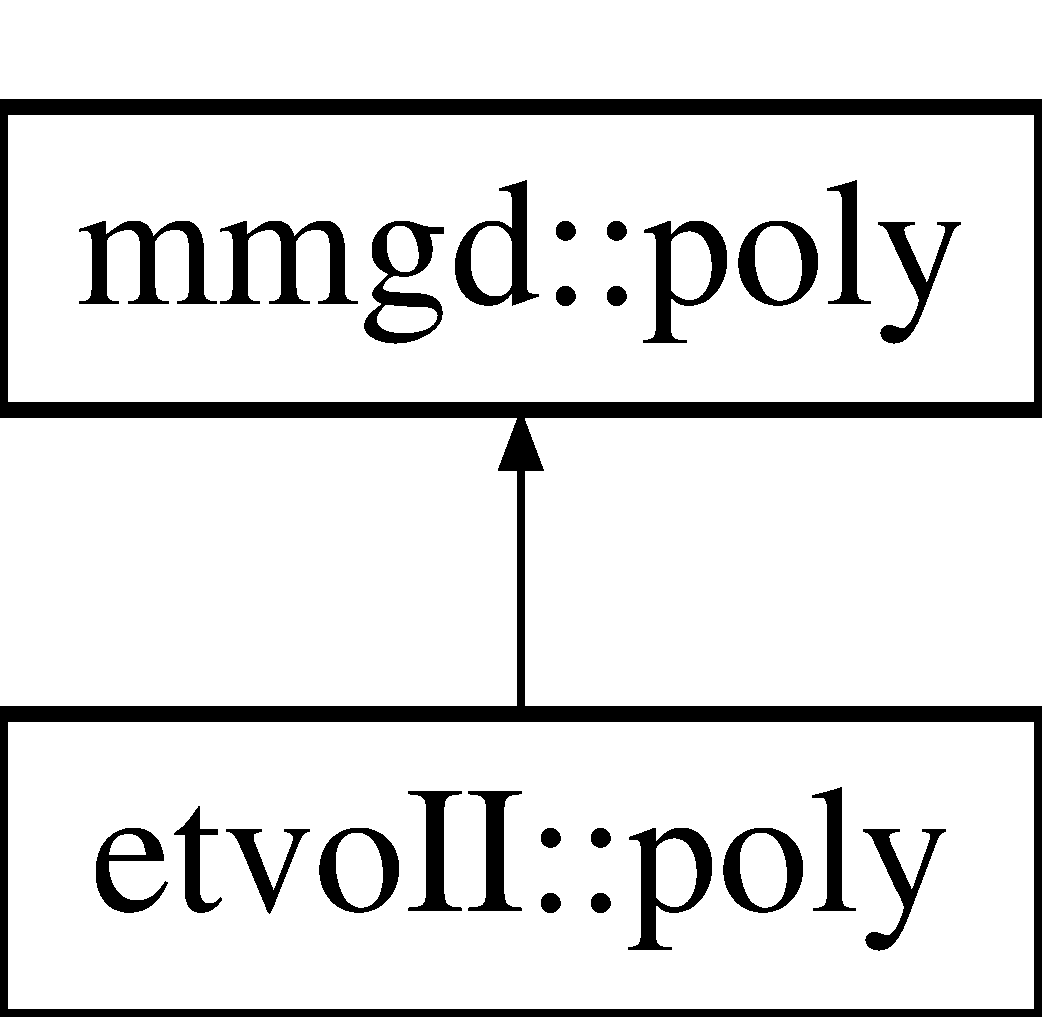
\includegraphics[height=2.000000cm]{classmmgd_1_1poly}
\end{center}
\end{figure}
\subsection*{Public Member Functions}
\begin{DoxyCompactItemize}
\item 
\mbox{\Hypertarget{classmmgd_1_1poly_aeda6ade4af424598ef30767c990a6dea}\label{classmmgd_1_1poly_aeda6ade4af424598ef30767c990a6dea}} 
{\bfseries poly} (const \mbox{\hyperlink{classmmgd_1_1poly}{poly}} \&)
\item 
\mbox{\Hypertarget{classmmgd_1_1poly_ad382086366b79f689dbd7928ecdfdbb5}\label{classmmgd_1_1poly_ad382086366b79f689dbd7928ecdfdbb5}} 
{\bfseries poly} (const \mbox{\hyperlink{classmmgd_1_1gd}{gd}} \&)
\item 
\mbox{\Hypertarget{classmmgd_1_1poly_a133a3b2591c6b3a15a4d4fe03ef3599c}\label{classmmgd_1_1poly_a133a3b2591c6b3a15a4d4fe03ef3599c}} 
{\bfseries poly} (long g, long d)
\item 
\mbox{\Hypertarget{classmmgd_1_1poly_a06487929da588e96a1f63503bad5cd9d}\label{classmmgd_1_1poly_a06487929da588e96a1f63503bad5cd9d}} 
{\bfseries poly} (unsigned int, \mbox{\hyperlink{classmmgd_1_1gd}{gd}} $\ast$)
\item 
\mbox{\Hypertarget{classmmgd_1_1poly_ac9ae9acd1a5d97c73856ff68aaa8f509}\label{classmmgd_1_1poly_ac9ae9acd1a5d97c73856ff68aaa8f509}} 
\mbox{\hyperlink{classmmgd_1_1poly}{poly}} \& {\bfseries operator=} (const \mbox{\hyperlink{classmmgd_1_1poly}{poly}} \&)
\item 
\mbox{\Hypertarget{classmmgd_1_1poly_a593698e5f78e7aa64a143c85c35333f9}\label{classmmgd_1_1poly_a593698e5f78e7aa64a143c85c35333f9}} 
\mbox{\hyperlink{classmmgd_1_1poly}{poly}} \& {\bfseries operator()} (long g, long d)
\item 
\mbox{\Hypertarget{classmmgd_1_1poly_a5d092e747d276a8f38461a0b7d459759}\label{classmmgd_1_1poly_a5d092e747d276a8f38461a0b7d459759}} 
void {\bfseries init} (unsigned int, \mbox{\hyperlink{classmmgd_1_1gd}{gd}} $\ast$, int)
\item 
\mbox{\Hypertarget{classmmgd_1_1poly_aec0dc14f9919d62e2223afb9844d1f08}\label{classmmgd_1_1poly_aec0dc14f9919d62e2223afb9844d1f08}} 
\mbox{\hyperlink{classmmgd_1_1poly}{poly}} \& {\bfseries operator=} (const \mbox{\hyperlink{classmmgd_1_1gd}{gd}} \&gd1)
\item 
\mbox{\Hypertarget{classmmgd_1_1poly_a5bd23732151750b7e29789f6e17b9f6b}\label{classmmgd_1_1poly_a5bd23732151750b7e29789f6e17b9f6b}} 
\mbox{\hyperlink{classmmgd_1_1poly}{poly}} \& {\bfseries init} (long g, long d)
\item 
\mbox{\Hypertarget{classmmgd_1_1poly_ad8b13c9086778f9461ae8460ecca0d28}\label{classmmgd_1_1poly_ad8b13c9086778f9461ae8460ecca0d28}} 
void {\bfseries affecte} (unsigned int, const \mbox{\hyperlink{classmmgd_1_1gd}{gd}} $\ast$, unsigned int propre)
\item 
\mbox{\Hypertarget{classmmgd_1_1poly_ae5b5e62d2e6a5a820b71f939f4d06872}\label{classmmgd_1_1poly_ae5b5e62d2e6a5a820b71f939f4d06872}} 
\mbox{\hyperlink{classmmgd_1_1gd}{gd}} \& {\bfseries getpol} (int i) const
\item 
\mbox{\Hypertarget{classmmgd_1_1poly_a2f4f968f61c7af5aff9e349f65d0da23}\label{classmmgd_1_1poly_a2f4f968f61c7af5aff9e349f65d0da23}} 
unsigned int {\bfseries getn} () const
\item 
\mbox{\Hypertarget{classmmgd_1_1poly_a5495fb6ca0d7c61bb5b206f559ffcf01}\label{classmmgd_1_1poly_a5495fb6ca0d7c61bb5b206f559ffcf01}} 
void {\bfseries setsimple} ()
\item 
\mbox{\Hypertarget{classmmgd_1_1poly_a18c1e001f43ce42745d7b2be6890cc3f}\label{classmmgd_1_1poly_a18c1e001f43ce42745d7b2be6890cc3f}} 
\mbox{\hyperlink{classmmgd_1_1gd}{gd}} $\ast$ {\bfseries getdata} ()
\item 
\mbox{\Hypertarget{classmmgd_1_1poly_a184a9b26eed443676f8d55919856a363}\label{classmmgd_1_1poly_a184a9b26eed443676f8d55919856a363}} 
void {\bfseries popj} (unsigned int j)
\item 
\mbox{\Hypertarget{classmmgd_1_1poly_a8b72b2a38fe605ee83d03c546315feaa}\label{classmmgd_1_1poly_a8b72b2a38fe605ee83d03c546315feaa}} 
void {\bfseries pop} ()
\item 
\mbox{\Hypertarget{classmmgd_1_1poly_a0b40ee1475cd9d321ddea43dde871321}\label{classmmgd_1_1poly_a0b40ee1475cd9d321ddea43dde871321}} 
void {\bfseries add} (const \mbox{\hyperlink{classmmgd_1_1gd}{gd}} \&m1)
\item 
\mbox{\Hypertarget{classmmgd_1_1poly_a49ff0c355621ee90b83986b5c21a681b}\label{classmmgd_1_1poly_a49ff0c355621ee90b83986b5c21a681b}} 
void {\bfseries simpli} ()
\item 
\mbox{\Hypertarget{classmmgd_1_1poly_a7c0e2e60fb473ecd70af742d6cfb8214}\label{classmmgd_1_1poly_a7c0e2e60fb473ecd70af742d6cfb8214}} 
void {\bfseries onlysimpli} ()
\item 
\mbox{\Hypertarget{classmmgd_1_1poly_a5033ce10a8708ca2a6d43d31ac0abb70}\label{classmmgd_1_1poly_a5033ce10a8708ca2a6d43d31ac0abb70}} 
void {\bfseries swapgd} (\mbox{\hyperlink{classmmgd_1_1gd}{gd}} \&a, \mbox{\hyperlink{classmmgd_1_1gd}{gd}} \&b)
\item 
\mbox{\Hypertarget{classmmgd_1_1poly_ab3bd363ed00bc3be3d31b0e9e79debde}\label{classmmgd_1_1poly_ab3bd363ed00bc3be3d31b0e9e79debde}} 
int {\bfseries partitionner} (\mbox{\hyperlink{classmmgd_1_1gd}{gd}} $\ast$tab, int debut, int dernier, int pivot, int comp(const void $\ast$, const void $\ast$))
\item 
\mbox{\Hypertarget{classmmgd_1_1poly_ae121ae3e10e8252bc9b9c1b745867a8b}\label{classmmgd_1_1poly_ae121ae3e10e8252bc9b9c1b745867a8b}} 
int {\bfseries operator==} (const \mbox{\hyperlink{classmmgd_1_1poly}{poly}} \&)
\end{DoxyCompactItemize}
\subsection*{Static Public Attributes}
\begin{DoxyCompactItemize}
\item 
\mbox{\Hypertarget{classmmgd_1_1poly_a4c658d3ff941048a220fe08f3bc2dfab}\label{classmmgd_1_1poly_a4c658d3ff941048a220fe08f3bc2dfab}} 
static int {\bfseries forcage} =0
\end{DoxyCompactItemize}
\subsection*{Friends}
\begin{DoxyCompactItemize}
\item 
\mbox{\Hypertarget{classmmgd_1_1poly_a902bbbf11a23a3fc4075dcd29e9ba0a3}\label{classmmgd_1_1poly_a902bbbf11a23a3fc4075dcd29e9ba0a3}} 
int {\bfseries compgd} (const void $\ast$p1, const void $\ast$p2)
\item 
\mbox{\Hypertarget{classmmgd_1_1poly_a6e11338fa76cb7916e75802534f77587}\label{classmmgd_1_1poly_a6e11338fa76cb7916e75802534f77587}} 
void {\bfseries qsort\+\_\+gd} (\mbox{\hyperlink{classmmgd_1_1gd}{gd}} $\ast$adtab, int premier, int dernier, int comp(const void $\ast$, const void $\ast$))
\item 
\mbox{\Hypertarget{classmmgd_1_1poly_abcce92100cdf3208f275859d3908fbe6}\label{classmmgd_1_1poly_abcce92100cdf3208f275859d3908fbe6}} 
\mbox{\hyperlink{classmmgd_1_1poly}{poly}} {\bfseries oplus} (\mbox{\hyperlink{classmmgd_1_1poly}{poly}} \&, \mbox{\hyperlink{classmmgd_1_1poly}{poly}} \&)
\item 
\mbox{\Hypertarget{classmmgd_1_1poly_a247e64e536c6f1a070bc8eb9d870058d}\label{classmmgd_1_1poly_a247e64e536c6f1a070bc8eb9d870058d}} 
\mbox{\hyperlink{classmmgd_1_1poly}{poly}} {\bfseries oplus} (\mbox{\hyperlink{classmmgd_1_1gd}{gd}} \&, \mbox{\hyperlink{classmmgd_1_1gd}{gd}} \&)
\item 
\mbox{\Hypertarget{classmmgd_1_1poly_a8408c8cbe50239231608be92b6c8b47f}\label{classmmgd_1_1poly_a8408c8cbe50239231608be92b6c8b47f}} 
\mbox{\hyperlink{classmmgd_1_1poly}{poly}} {\bfseries oplus} (\mbox{\hyperlink{classmmgd_1_1poly}{poly}} \&, \mbox{\hyperlink{classmmgd_1_1gd}{gd}} \&)
\item 
\mbox{\Hypertarget{classmmgd_1_1poly_a7d137100cfb94e8231c00c253b1c0d45}\label{classmmgd_1_1poly_a7d137100cfb94e8231c00c253b1c0d45}} 
\mbox{\hyperlink{classmmgd_1_1poly}{poly}} {\bfseries oplus} (\mbox{\hyperlink{classmmgd_1_1gd}{gd}} \&, \mbox{\hyperlink{classmmgd_1_1poly}{poly}} \&)
\item 
\mbox{\Hypertarget{classmmgd_1_1poly_aa457431adea4b51f375222c772dfa926}\label{classmmgd_1_1poly_aa457431adea4b51f375222c772dfa926}} 
\mbox{\hyperlink{classmmgd_1_1poly}{poly}} {\bfseries oplus} (\mbox{\hyperlink{classmmgd_1_1poly}{poly}} \&, \mbox{\hyperlink{classmmgd_1_1poly}{poly}} \&, \mbox{\hyperlink{classmmgd_1_1poly}{poly}} \&)
\item 
\mbox{\Hypertarget{classmmgd_1_1poly_a035bd6940202bdaefbd9f15b65aca4c7}\label{classmmgd_1_1poly_a035bd6940202bdaefbd9f15b65aca4c7}} 
\mbox{\hyperlink{classmmgd_1_1poly}{poly}} {\bfseries oplus} (\mbox{\hyperlink{classmmgd_1_1poly}{poly}} \&, \mbox{\hyperlink{classmmgd_1_1poly}{poly}} \&, \mbox{\hyperlink{classmmgd_1_1poly}{poly}} \&, \mbox{\hyperlink{classmmgd_1_1poly}{poly}} \&)
\item 
\mbox{\Hypertarget{classmmgd_1_1poly_adc4c4b3ff5bde03992056d6293de8adc}\label{classmmgd_1_1poly_adc4c4b3ff5bde03992056d6293de8adc}} 
\mbox{\hyperlink{classmmgd_1_1poly}{poly}} {\bfseries otimes} (\mbox{\hyperlink{classmmgd_1_1poly}{poly}} \&poly1, \mbox{\hyperlink{classmmgd_1_1poly}{poly}} \&poly2)
\item 
\mbox{\Hypertarget{classmmgd_1_1poly_ab6880d5f38b5617b51b536cc12dbe632}\label{classmmgd_1_1poly_ab6880d5f38b5617b51b536cc12dbe632}} 
\mbox{\hyperlink{classmmgd_1_1poly}{poly}} {\bfseries otimes} (\mbox{\hyperlink{classmmgd_1_1poly}{poly}} \&poly1, \mbox{\hyperlink{classmmgd_1_1gd}{gd}} \&gd2)
\item 
\mbox{\Hypertarget{classmmgd_1_1poly_a48427a3900629c5a386cbc2817f16e55}\label{classmmgd_1_1poly_a48427a3900629c5a386cbc2817f16e55}} 
\mbox{\hyperlink{classmmgd_1_1poly}{poly}} {\bfseries otimes} (\mbox{\hyperlink{classmmgd_1_1gd}{gd}} \&gd1, \mbox{\hyperlink{classmmgd_1_1poly}{poly}} \&poly2)
\item 
\mbox{\Hypertarget{classmmgd_1_1poly_a803937f55e9be138336bd21748fea019}\label{classmmgd_1_1poly_a803937f55e9be138336bd21748fea019}} 
\mbox{\hyperlink{classmmgd_1_1poly}{poly}} {\bfseries inf} (\mbox{\hyperlink{classmmgd_1_1poly}{poly}} \&poly1, \mbox{\hyperlink{classmmgd_1_1poly}{poly}} \&poly2)
\item 
\mbox{\Hypertarget{classmmgd_1_1poly_a03fcc1a1d0999a26f741958726ad8786}\label{classmmgd_1_1poly_a03fcc1a1d0999a26f741958726ad8786}} 
\mbox{\hyperlink{classmmgd_1_1poly}{poly}} {\bfseries inf} (\mbox{\hyperlink{classmmgd_1_1poly}{poly}} \&poly1, \mbox{\hyperlink{classmmgd_1_1gd}{gd}} \&gd2)
\item 
\mbox{\Hypertarget{classmmgd_1_1poly_a201336586d8f06607e606a71d56d0620}\label{classmmgd_1_1poly_a201336586d8f06607e606a71d56d0620}} 
\mbox{\hyperlink{classmmgd_1_1poly}{poly}} {\bfseries inf} (\mbox{\hyperlink{classmmgd_1_1gd}{gd}} \&gd1, \mbox{\hyperlink{classmmgd_1_1poly}{poly}} \&poly2)
\item 
\mbox{\Hypertarget{classmmgd_1_1poly_a1ca2365b15ec5d9647e2ee8cc82bc0c3}\label{classmmgd_1_1poly_a1ca2365b15ec5d9647e2ee8cc82bc0c3}} 
\mbox{\hyperlink{classmmgd_1_1poly}{poly}} {\bfseries frac} (\mbox{\hyperlink{classmmgd_1_1poly}{poly}} \&poly1, \mbox{\hyperlink{classmmgd_1_1gd}{gd}} \&gd2)
\item 
\mbox{\Hypertarget{classmmgd_1_1poly_a2bb496ce83846bee4b6273821e059827}\label{classmmgd_1_1poly_a2bb496ce83846bee4b6273821e059827}} 
\mbox{\hyperlink{classmmgd_1_1poly}{poly}} {\bfseries frac} (\mbox{\hyperlink{classmmgd_1_1poly}{poly}} \&poly1, \mbox{\hyperlink{classmmgd_1_1poly}{poly}} \&poly2)
\item 
\mbox{\Hypertarget{classmmgd_1_1poly_af8dd7f52f6fa54f4f40d657652b14a54}\label{classmmgd_1_1poly_af8dd7f52f6fa54f4f40d657652b14a54}} 
\mbox{\hyperlink{classmmgd_1_1poly}{poly}} {\bfseries frac} (\mbox{\hyperlink{classmmgd_1_1gd}{gd}} \&gd1, \mbox{\hyperlink{classmmgd_1_1poly}{poly}} \&poly2)
\item 
\mbox{\Hypertarget{classmmgd_1_1poly_ad9580516418e4c9c5ee22b7f67cfb6ee}\label{classmmgd_1_1poly_ad9580516418e4c9c5ee22b7f67cfb6ee}} 
\mbox{\hyperlink{classmmgd_1_1poly}{poly}} {\bfseries prcaus} (\mbox{\hyperlink{classmmgd_1_1poly}{poly}} \&)
\item 
\mbox{\Hypertarget{classmmgd_1_1poly_a0361c355a8ea5d7e13ec20144390082f}\label{classmmgd_1_1poly_a0361c355a8ea5d7e13ec20144390082f}} 
std\+::ostream \& {\bfseries operator$<$$<$} (std\+::ostream \&, \mbox{\hyperlink{classmmgd_1_1poly}{poly}} \&)
\item 
\mbox{\Hypertarget{classmmgd_1_1poly_af0ab9a74b034ed507c6070d9a47951b8}\label{classmmgd_1_1poly_af0ab9a74b034ed507c6070d9a47951b8}} 
std\+::fstream \& {\bfseries operator$<$$<$} (std\+::fstream \&, \mbox{\hyperlink{classmmgd_1_1poly}{poly}} \&)
\item 
\mbox{\Hypertarget{classmmgd_1_1poly_a9cecbf55fe370b38e24b8b639fd1ee03}\label{classmmgd_1_1poly_a9cecbf55fe370b38e24b8b639fd1ee03}} 
\mbox{\hyperlink{classmmgd_1_1poly}{poly}} {\bfseries odot} (const \mbox{\hyperlink{classmmgd_1_1poly}{poly}} \&poly1, const \mbox{\hyperlink{classmmgd_1_1poly}{poly}} \&poly2)
\item 
\mbox{\Hypertarget{classmmgd_1_1poly_aff323f3e36b51b89ff4b52ffdf7464dd}\label{classmmgd_1_1poly_aff323f3e36b51b89ff4b52ffdf7464dd}} 
\mbox{\hyperlink{classmmgd_1_1poly}{poly}} {\bfseries fracodotsharp} (\mbox{\hyperlink{classmmgd_1_1poly}{poly}} \&poly1, \mbox{\hyperlink{classmmgd_1_1poly}{poly}} \&poly2)
\item 
\mbox{\Hypertarget{classmmgd_1_1poly_ad284d1dbb550ed9c6a6ad3f9f3e2e3cc}\label{classmmgd_1_1poly_ad284d1dbb550ed9c6a6ad3f9f3e2e3cc}} 
\mbox{\hyperlink{classmmgd_1_1poly}{poly}} {\bfseries fracodotflat} (\mbox{\hyperlink{classmmgd_1_1poly}{poly}} \&poly1, \mbox{\hyperlink{classmmgd_1_1poly}{poly}} \&poly2)
\end{DoxyCompactItemize}


The documentation for this class was generated from the following files\+:\begin{DoxyCompactItemize}
\item 
etvo/minmaxgd/poly.\+h\item 
etvo/minmaxgd/poly.\+cpp\end{DoxyCompactItemize}

\hypertarget{classetvo_i_i_1_1poly}{}\section{etvo\+II\+:\+:poly Class Reference}
\label{classetvo_i_i_1_1poly}\index{etvo\+I\+I\+::poly@{etvo\+I\+I\+::poly}}
Inheritance diagram for etvo\+II\+:\+:poly\+:\begin{figure}[H]
\begin{center}
\leavevmode
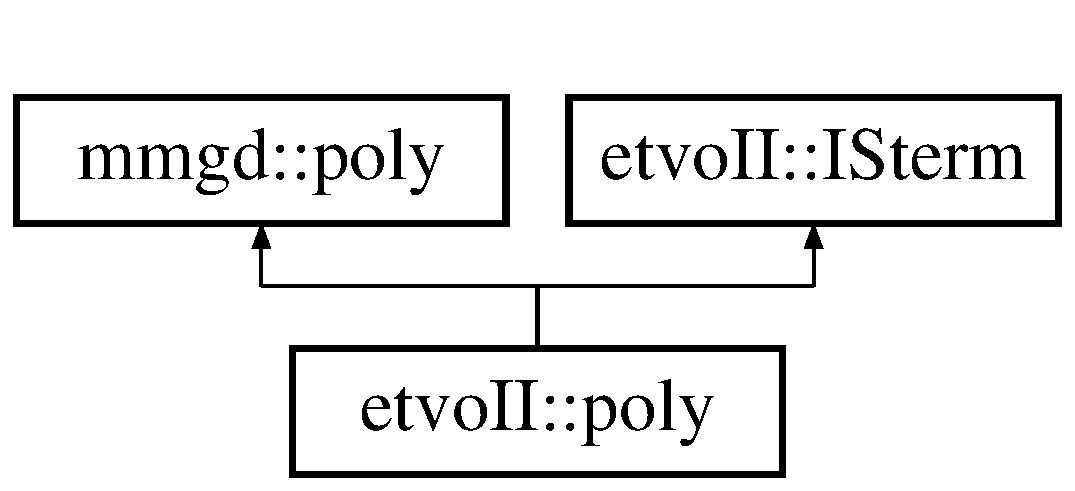
\includegraphics[height=2.000000cm]{classetvo_i_i_1_1poly}
\end{center}
\end{figure}
\subsection*{Public Member Functions}
\begin{DoxyCompactItemize}
\item 
\mbox{\Hypertarget{classetvo_i_i_1_1poly_a353bfb20ce3f36a59c33daca14d1892c}\label{classetvo_i_i_1_1poly_a353bfb20ce3f36a59c33daca14d1892c}} 
bool {\bfseries is\+Epsilon} () const
\item 
\mbox{\Hypertarget{classetvo_i_i_1_1poly_a0e60bb5d6fef4a0d54099f65672b5ae8}\label{classetvo_i_i_1_1poly_a0e60bb5d6fef4a0d54099f65672b5ae8}} 
{\bfseries poly} (bool Top\+NotE)
\item 
\mbox{\Hypertarget{classetvo_i_i_1_1poly_a1762ddb945535fbe929613e2bb1f39dc}\label{classetvo_i_i_1_1poly_a1762ddb945535fbe929613e2bb1f39dc}} 
{\bfseries poly} (const \mbox{\hyperlink{classetvo_i_i_1_1poly}{poly}} \&)
\item 
\mbox{\Hypertarget{classetvo_i_i_1_1poly_abc4a5b558c505c982d4a755ed0bb36c1}\label{classetvo_i_i_1_1poly_abc4a5b558c505c982d4a755ed0bb36c1}} 
{\bfseries poly} (const \mbox{\hyperlink{classetvo_i_i_1_1gd}{gd}} \&)
\item 
\mbox{\Hypertarget{classetvo_i_i_1_1poly_aa321444d01a4172e3d22b92555983004}\label{classetvo_i_i_1_1poly_aa321444d01a4172e3d22b92555983004}} 
{\bfseries poly} (const \mbox{\hyperlink{classmmgd_1_1poly}{mmgd\+::poly}} \&p)
\item 
\mbox{\Hypertarget{classetvo_i_i_1_1poly_a367aed21018a2bd216caf41655d034d1}\label{classetvo_i_i_1_1poly_a367aed21018a2bd216caf41655d034d1}} 
{\bfseries poly} (long g, long d)
\item 
\mbox{\Hypertarget{classetvo_i_i_1_1poly_a4234613f4b26238a03af66cef2ff31aa}\label{classetvo_i_i_1_1poly_a4234613f4b26238a03af66cef2ff31aa}} 
{\bfseries poly} (const std\+::vector$<$ \mbox{\hyperlink{classmmgd_1_1gd}{mmgd\+::gd}} $>$ \&v)
\item 
\mbox{\hyperlink{classetvo_i_i_1_1poly_ae6a829a66995bc2fe54024c96dc23c24}{poly}} (const std\+::vector$<$ \mbox{\hyperlink{classetvo_i_i_1_1gd}{gd}} $>$ \&v)
\item 
\mbox{\Hypertarget{classetvo_i_i_1_1poly_a1710fc7eabe9e7466f421c829a9e2a2a}\label{classetvo_i_i_1_1poly_a1710fc7eabe9e7466f421c829a9e2a2a}} 
void {\bfseries add} (const \mbox{\hyperlink{classetvo_i_i_1_1gd}{gd}} \&m)
\item 
\mbox{\Hypertarget{classetvo_i_i_1_1poly_a92c17ebde40549708b5d8d088b48f3cb}\label{classetvo_i_i_1_1poly_a92c17ebde40549708b5d8d088b48f3cb}} 
\mbox{\hyperlink{classetvo_i_i_1_1gd}{gd}} {\bfseries operator\mbox{[}$\,$\mbox{]}} (unsigned i) const
\item 
\mbox{\Hypertarget{classetvo_i_i_1_1poly_af9ccac57a1ae1947aeee5c5a04e283db}\label{classetvo_i_i_1_1poly_af9ccac57a1ae1947aeee5c5a04e283db}} 
\mbox{\hyperlink{classetvo_i_i_1_1poly}{poly}} \& {\bfseries operator=} (const \mbox{\hyperlink{classetvo_i_i_1_1poly}{poly}} \&p)
\item 
\mbox{\Hypertarget{classetvo_i_i_1_1poly_a95fb66a60f73cb682cc8e31774e83a47}\label{classetvo_i_i_1_1poly_a95fb66a60f73cb682cc8e31774e83a47}} 
\mbox{\hyperlink{classetvo_i_i_1_1poly}{poly}} \& {\bfseries operator=} (const \mbox{\hyperlink{classetvo_i_i_1_1gd}{gd}} \&m)
\item 
\mbox{\Hypertarget{classetvo_i_i_1_1poly_af50a93ff94c09153c4a4205d19d0260a}\label{classetvo_i_i_1_1poly_af50a93ff94c09153c4a4205d19d0260a}} 
bool {\bfseries operator==} (const \mbox{\hyperlink{classetvo_i_i_1_1poly}{poly}} \&p) const
\item 
\mbox{\Hypertarget{classetvo_i_i_1_1poly_a93e1e1bf7f5bd8609c01209ae5e5fe89}\label{classetvo_i_i_1_1poly_a93e1e1bf7f5bd8609c01209ae5e5fe89}} 
bool {\bfseries operator$<$=} (const \mbox{\hyperlink{classetvo_i_i_1_1poly}{poly}} \&p) const
\item 
\mbox{\Hypertarget{classetvo_i_i_1_1poly_a6857c709afd01ea4c0b5a5443d9c5ba9}\label{classetvo_i_i_1_1poly_a6857c709afd01ea4c0b5a5443d9c5ba9}} 
bool {\bfseries operator$>$=} (const \mbox{\hyperlink{classetvo_i_i_1_1poly}{poly}} \&p) const
\item 
\mbox{\Hypertarget{classetvo_i_i_1_1poly_aa92f2a0b10df5e0d1906e19d849c340e}\label{classetvo_i_i_1_1poly_aa92f2a0b10df5e0d1906e19d849c340e}} 
\mbox{\hyperlink{classetvo_i_i_1_1poly}{poly}} {\bfseries operator+} (const \mbox{\hyperlink{classetvo_i_i_1_1poly}{poly}} \&p) const
\item 
\mbox{\Hypertarget{classetvo_i_i_1_1poly_aeb92d816c138071e4c06c0838cb8da72}\label{classetvo_i_i_1_1poly_aeb92d816c138071e4c06c0838cb8da72}} 
\mbox{\hyperlink{classetvo_i_i_1_1poly}{poly}} {\bfseries operator+} (const \mbox{\hyperlink{classetvo_i_i_1_1gd}{gd}} \&m) const
\item 
\mbox{\Hypertarget{classetvo_i_i_1_1poly_afed4491e22af7c9aadd9b1ad1a562fd8}\label{classetvo_i_i_1_1poly_afed4491e22af7c9aadd9b1ad1a562fd8}} 
\mbox{\hyperlink{classetvo_i_i_1_1poly}{poly}} {\bfseries operator$\ast$} (const \mbox{\hyperlink{classetvo_i_i_1_1poly}{poly}} \&p) const
\item 
\mbox{\Hypertarget{classetvo_i_i_1_1poly_a494b6d1aaa61396c7126ae0f3137897a}\label{classetvo_i_i_1_1poly_a494b6d1aaa61396c7126ae0f3137897a}} 
\mbox{\hyperlink{classetvo_i_i_1_1poly}{poly}} {\bfseries operator$\ast$} (const \mbox{\hyperlink{classetvo_i_i_1_1gd}{gd}} \&m) const
\item 
\mbox{\Hypertarget{classetvo_i_i_1_1poly_acaa48cefc9d3a74c252cad52c234416f}\label{classetvo_i_i_1_1poly_acaa48cefc9d3a74c252cad52c234416f}} 
\mbox{\hyperlink{classetvo_i_i_1_1poly}{poly}} {\bfseries inf} (const \mbox{\hyperlink{classetvo_i_i_1_1poly}{poly}} \&p) const
\item 
\mbox{\Hypertarget{classetvo_i_i_1_1poly_a5df0d14cd444a28530f6f39663afff27}\label{classetvo_i_i_1_1poly_a5df0d14cd444a28530f6f39663afff27}} 
\mbox{\hyperlink{classetvo_i_i_1_1poly}{poly}} {\bfseries inf} (const \mbox{\hyperlink{classetvo_i_i_1_1gd}{gd}} \&m) const
\item 
\mbox{\Hypertarget{classetvo_i_i_1_1poly_a22a0d088cc40aa41dfaf78cc07769aa2}\label{classetvo_i_i_1_1poly_a22a0d088cc40aa41dfaf78cc07769aa2}} 
\mbox{\hyperlink{classetvo_i_i_1_1poly}{poly}} {\bfseries lfrac} (const \mbox{\hyperlink{classetvo_i_i_1_1poly}{poly}} \&p) const
\item 
\mbox{\Hypertarget{classetvo_i_i_1_1poly_adc09dbbb43f9875d4525f407818c68ba}\label{classetvo_i_i_1_1poly_adc09dbbb43f9875d4525f407818c68ba}} 
\mbox{\hyperlink{classetvo_i_i_1_1poly}{poly}} {\bfseries rfrac} (const \mbox{\hyperlink{classetvo_i_i_1_1poly}{poly}} \&p) const
\item 
\mbox{\Hypertarget{classetvo_i_i_1_1poly_ad785794b0e7392a93767e77f59695e38}\label{classetvo_i_i_1_1poly_ad785794b0e7392a93767e77f59695e38}} 
\mbox{\hyperlink{classetvo_i_i_1_1poly}{poly}} {\bfseries frac} (const \mbox{\hyperlink{classetvo_i_i_1_1poly}{poly}} \&p) const
\item 
\mbox{\Hypertarget{classetvo_i_i_1_1poly_a1f647dbcbc5adadde24f4206363e5b75}\label{classetvo_i_i_1_1poly_a1f647dbcbc5adadde24f4206363e5b75}} 
\mbox{\hyperlink{classetvo_i_i_1_1poly}{poly}} {\bfseries frac} (const \mbox{\hyperlink{classetvo_i_i_1_1gd}{gd}} \&m) const
\item 
\mbox{\Hypertarget{classetvo_i_i_1_1poly_a9b76e1797e23249124ea7a8d1c0b9269}\label{classetvo_i_i_1_1poly_a9b76e1797e23249124ea7a8d1c0b9269}} 
\mbox{\hyperlink{classetvo_i_i_1_1series}{series}} {\bfseries star} () const
\item 
\mbox{\Hypertarget{classetvo_i_i_1_1poly_ac742906503aad7d42a88229397195103}\label{classetvo_i_i_1_1poly_ac742906503aad7d42a88229397195103}} 
\mbox{\hyperlink{classetvo_i_i_1_1poly}{poly}} {\bfseries prcaus} () const
\item 
\mbox{\Hypertarget{classetvo_i_i_1_1poly_a0b3abe28ff1af7704983917b5ff6e50b}\label{classetvo_i_i_1_1poly_a0b3abe28ff1af7704983917b5ff6e50b}} 
std\+::string {\bfseries To\+String} () const
\end{DoxyCompactItemize}
\subsection*{Static Public Member Functions}
\begin{DoxyCompactItemize}
\item 
\mbox{\Hypertarget{classetvo_i_i_1_1poly_a418ab66b51e7537f9d631b5635f94e9e}\label{classetvo_i_i_1_1poly_a418ab66b51e7537f9d631b5635f94e9e}} 
static \mbox{\hyperlink{classetvo_i_i_1_1poly}{poly}} {\bfseries Epsilon} ()
\item 
\mbox{\Hypertarget{classetvo_i_i_1_1poly_a5b100fc773873e32030033198fc8559a}\label{classetvo_i_i_1_1poly_a5b100fc773873e32030033198fc8559a}} 
static \mbox{\hyperlink{classetvo_i_i_1_1poly}{poly}} {\bfseries E} ()
\item 
\mbox{\Hypertarget{classetvo_i_i_1_1poly_a3c5589c416c9ac1651c2ad706d8dfd51}\label{classetvo_i_i_1_1poly_a3c5589c416c9ac1651c2ad706d8dfd51}} 
static \mbox{\hyperlink{classetvo_i_i_1_1poly}{poly}} {\bfseries Top} ()
\end{DoxyCompactItemize}
\subsection*{Additional Inherited Members}


\subsection{Constructor \& Destructor Documentation}
\mbox{\Hypertarget{classetvo_i_i_1_1poly_ae6a829a66995bc2fe54024c96dc23c24}\label{classetvo_i_i_1_1poly_ae6a829a66995bc2fe54024c96dc23c24}} 
\index{etvo\+I\+I\+::poly@{etvo\+I\+I\+::poly}!poly@{poly}}
\index{poly@{poly}!etvo\+I\+I\+::poly@{etvo\+I\+I\+::poly}}
\subsubsection{\texorpdfstring{poly()}{poly()}}
{\footnotesize\ttfamily etvo\+I\+I\+::poly\+::poly (\begin{DoxyParamCaption}\item[{const std\+::vector$<$ \mbox{\hyperlink{classetvo_i_i_1_1gd}{gd}} $>$ \&}]{v }\end{DoxyParamCaption})}

create a poly with the previous constr. 

The documentation for this class was generated from the following files\+:\begin{DoxyCompactItemize}
\item 
etvo/wrapper\+M\+M\+G\+D/poly\+Wrapper.\+h\item 
etvo/wrapper\+M\+M\+G\+D/poly\+Wrapper.\+cpp\end{DoxyCompactItemize}

\hypertarget{classetvo_i_i_1_1poly_ed}{}\section{etvo\+II\+:\+:poly\+Ed Class Reference}
\label{classetvo_i_i_1_1poly_ed}\index{etvo\+I\+I\+::poly\+Ed@{etvo\+I\+I\+::poly\+Ed}}
Inheritance diagram for etvo\+II\+:\+:poly\+Ed\+:\begin{figure}[H]
\begin{center}
\leavevmode
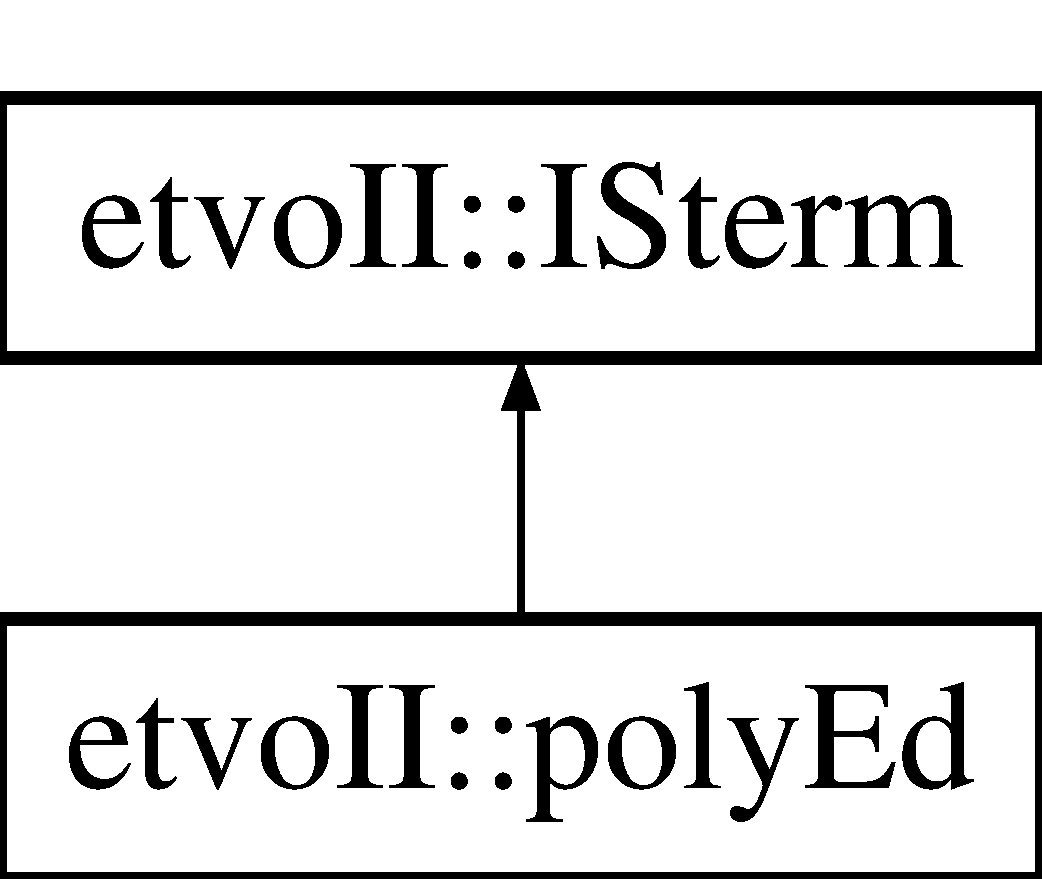
\includegraphics[height=2.000000cm]{classetvo_i_i_1_1poly_ed}
\end{center}
\end{figure}
\subsection*{Public Member Functions}
\begin{DoxyCompactItemize}
\item 
\mbox{\Hypertarget{classetvo_i_i_1_1poly_ed_a1f196af469b883ae567c2b024e0bf340}\label{classetvo_i_i_1_1poly_ed_a1f196af469b883ae567c2b024e0bf340}} 
{\bfseries poly\+Ed} (bool Top\+NotE)
\item 
\mbox{\Hypertarget{classetvo_i_i_1_1poly_ed_a2129297d769b8567d732413376c9a056}\label{classetvo_i_i_1_1poly_ed_a2129297d769b8567d732413376c9a056}} 
{\bfseries poly\+Ed} (const \mbox{\hyperlink{classetvo_i_i_1_1_ed}{Ed}} \&m)
\item 
\mbox{\Hypertarget{classetvo_i_i_1_1poly_ed_ab66e44a8b466d0de444a4e512fe489cc}\label{classetvo_i_i_1_1poly_ed_ab66e44a8b466d0de444a4e512fe489cc}} 
{\bfseries poly\+Ed} (const std\+::vector$<$ \mbox{\hyperlink{classetvo_i_i_1_1_ed}{Ed}} $>$ \&)
\item 
\mbox{\Hypertarget{classetvo_i_i_1_1poly_ed_acf74bead77c2d405dae3ab0fa79c6146}\label{classetvo_i_i_1_1poly_ed_acf74bead77c2d405dae3ab0fa79c6146}} 
\mbox{\hyperlink{classetvo_i_i_1_1poly}{poly}} {\bfseries to\+Poly} () const
\item 
\mbox{\Hypertarget{classetvo_i_i_1_1poly_ed_adeb4c6b9787fd9c09e5b4321873e543d}\label{classetvo_i_i_1_1poly_ed_adeb4c6b9787fd9c09e5b4321873e543d}} 
\mbox{\hyperlink{classetvo_i_i_1_1poly_ed}{poly\+Ed}} {\bfseries operator+} (const \mbox{\hyperlink{classetvo_i_i_1_1poly_ed}{poly\+Ed}} \&p) const
\item 
\mbox{\Hypertarget{classetvo_i_i_1_1poly_ed_ab0185415cab37365b9f252227e7271f7}\label{classetvo_i_i_1_1poly_ed_ab0185415cab37365b9f252227e7271f7}} 
\mbox{\hyperlink{classetvo_i_i_1_1poly_ed}{poly\+Ed}} {\bfseries oplus} (const \mbox{\hyperlink{classetvo_i_i_1_1poly_ed}{poly\+Ed}} \&p) const
\item 
\mbox{\Hypertarget{classetvo_i_i_1_1poly_ed_ad1b56f93a4fca155110c5f2f3bcf5aa3}\label{classetvo_i_i_1_1poly_ed_ad1b56f93a4fca155110c5f2f3bcf5aa3}} 
\mbox{\hyperlink{classetvo_i_i_1_1poly_ed}{poly\+Ed}} {\bfseries oplus\+CD} (const \mbox{\hyperlink{classetvo_i_i_1_1poly_ed}{poly\+Ed}} \&p) const
\item 
\mbox{\Hypertarget{classetvo_i_i_1_1poly_ed_a8a03100c98b2e060ac4ed8594e2bf624}\label{classetvo_i_i_1_1poly_ed_a8a03100c98b2e060ac4ed8594e2bf624}} 
\mbox{\hyperlink{classetvo_i_i_1_1poly_ed}{poly\+Ed}} {\bfseries operator+} (const \mbox{\hyperlink{classetvo_i_i_1_1_ed}{Ed}} \&m) const
\item 
\mbox{\Hypertarget{classetvo_i_i_1_1poly_ed_ac982c8af4cb0a52dbded07dd1f33f183}\label{classetvo_i_i_1_1poly_ed_ac982c8af4cb0a52dbded07dd1f33f183}} 
void {\bfseries add} (const \mbox{\hyperlink{classetvo_i_i_1_1_ed}{Ed}} \&m)
\item 
\mbox{\Hypertarget{classetvo_i_i_1_1poly_ed_ae75d2b9d0cd71f7c8629cf6b252651ac}\label{classetvo_i_i_1_1poly_ed_ae75d2b9d0cd71f7c8629cf6b252651ac}} 
\mbox{\hyperlink{classetvo_i_i_1_1poly_ed}{poly\+Ed}} {\bfseries operator$\ast$} (const \mbox{\hyperlink{classetvo_i_i_1_1poly_ed}{poly\+Ed}} \&p) const
\item 
\mbox{\Hypertarget{classetvo_i_i_1_1poly_ed_adcb55ea5c9bf5c39893bc6c740e74704}\label{classetvo_i_i_1_1poly_ed_adcb55ea5c9bf5c39893bc6c740e74704}} 
\mbox{\hyperlink{classetvo_i_i_1_1poly_ed}{poly\+Ed}} {\bfseries operator$\ast$} (const \mbox{\hyperlink{classetvo_i_i_1_1_ed}{Ed}} \&m) const
\item 
\mbox{\Hypertarget{classetvo_i_i_1_1poly_ed_a45892c5e5b356d7c5491b8c0fc982fef}\label{classetvo_i_i_1_1poly_ed_a45892c5e5b356d7c5491b8c0fc982fef}} 
\mbox{\hyperlink{classetvo_i_i_1_1poly_ed}{poly\+Ed}} {\bfseries otimes} (const \mbox{\hyperlink{classetvo_i_i_1_1poly_ed}{poly\+Ed}} \&p) const
\item 
\mbox{\Hypertarget{classetvo_i_i_1_1poly_ed_af7ae999d13b58a2f8ddb4fb3e95e37c2}\label{classetvo_i_i_1_1poly_ed_af7ae999d13b58a2f8ddb4fb3e95e37c2}} 
\mbox{\hyperlink{classetvo_i_i_1_1poly_ed}{poly\+Ed}} {\bfseries otimes\+CD} (const \mbox{\hyperlink{classetvo_i_i_1_1poly_ed}{poly\+Ed}} \&p) const
\item 
\mbox{\Hypertarget{classetvo_i_i_1_1poly_ed_a03eeb8b76f668f15b70898c8a99bd953}\label{classetvo_i_i_1_1poly_ed_a03eeb8b76f668f15b70898c8a99bd953}} 
\mbox{\hyperlink{classetvo_i_i_1_1poly_ed}{poly\+Ed}} {\bfseries inf} (const \mbox{\hyperlink{classetvo_i_i_1_1poly_ed}{poly\+Ed}} \&) const
\item 
\mbox{\Hypertarget{classetvo_i_i_1_1poly_ed_a37a71a5d8d47b3d02c61cf5fbddacb96}\label{classetvo_i_i_1_1poly_ed_a37a71a5d8d47b3d02c61cf5fbddacb96}} 
\mbox{\hyperlink{classetvo_i_i_1_1poly_ed}{poly\+Ed}} {\bfseries inf\+CD} (const \mbox{\hyperlink{classetvo_i_i_1_1poly_ed}{poly\+Ed}} \&) const
\item 
\mbox{\Hypertarget{classetvo_i_i_1_1poly_ed_a689f9cb8aa508dd783332e1c614dd4ab}\label{classetvo_i_i_1_1poly_ed_a689f9cb8aa508dd783332e1c614dd4ab}} 
\mbox{\hyperlink{classetvo_i_i_1_1series_ed}{series\+Ed}} {\bfseries star} () const
\item 
\mbox{\Hypertarget{classetvo_i_i_1_1poly_ed_af4edaa3b37ec578fcca36ab7fb05042f}\label{classetvo_i_i_1_1poly_ed_af4edaa3b37ec578fcca36ab7fb05042f}} 
\mbox{\hyperlink{classetvo_i_i_1_1poly_ed}{poly\+Ed}} {\bfseries lfrac} (const \mbox{\hyperlink{classetvo_i_i_1_1poly_ed}{poly\+Ed}} \&) const
\item 
\mbox{\Hypertarget{classetvo_i_i_1_1poly_ed_ad6cff67652a41965d0965a602f40e931}\label{classetvo_i_i_1_1poly_ed_ad6cff67652a41965d0965a602f40e931}} 
\mbox{\hyperlink{classetvo_i_i_1_1poly_ed}{poly\+Ed}} {\bfseries lfrac\+CD} (const \mbox{\hyperlink{classetvo_i_i_1_1poly_ed}{poly\+Ed}} \&) const
\item 
\mbox{\Hypertarget{classetvo_i_i_1_1poly_ed_aa6c04e5c4cee614fef3fa076a90b844f}\label{classetvo_i_i_1_1poly_ed_aa6c04e5c4cee614fef3fa076a90b844f}} 
\mbox{\hyperlink{classetvo_i_i_1_1poly_ed}{poly\+Ed}} {\bfseries lfrac} (const \mbox{\hyperlink{classetvo_i_i_1_1_ed}{Ed}} \&m) const
\item 
\mbox{\Hypertarget{classetvo_i_i_1_1poly_ed_a58764f59d783437a11c8e2917241f220}\label{classetvo_i_i_1_1poly_ed_a58764f59d783437a11c8e2917241f220}} 
\mbox{\hyperlink{classetvo_i_i_1_1poly_ed}{poly\+Ed}} {\bfseries rfrac} (const \mbox{\hyperlink{classetvo_i_i_1_1poly_ed}{poly\+Ed}} \&) const
\item 
\mbox{\Hypertarget{classetvo_i_i_1_1poly_ed_ad9fe3ff1012b67f3c8b7995be629a321}\label{classetvo_i_i_1_1poly_ed_ad9fe3ff1012b67f3c8b7995be629a321}} 
\mbox{\hyperlink{classetvo_i_i_1_1poly_ed}{poly\+Ed}} {\bfseries rfrac\+CD} (const \mbox{\hyperlink{classetvo_i_i_1_1poly_ed}{poly\+Ed}} \&) const
\item 
\mbox{\Hypertarget{classetvo_i_i_1_1poly_ed_a2bc172be3677d61a6771ba4a47ce3b05}\label{classetvo_i_i_1_1poly_ed_a2bc172be3677d61a6771ba4a47ce3b05}} 
\mbox{\hyperlink{classetvo_i_i_1_1poly_ed}{poly\+Ed}} {\bfseries rfrac} (const \mbox{\hyperlink{classetvo_i_i_1_1_ed}{Ed}} \&m) const
\item 
\mbox{\Hypertarget{classetvo_i_i_1_1poly_ed_abf15216ada869fad086e9d4c9f7bf4ec}\label{classetvo_i_i_1_1poly_ed_abf15216ada869fad086e9d4c9f7bf4ec}} 
bool {\bfseries operator==} (const \mbox{\hyperlink{classetvo_i_i_1_1poly_ed}{poly\+Ed}} \&) const
\item 
\mbox{\Hypertarget{classetvo_i_i_1_1poly_ed_a2714800955c124fda4ecff8f89f8db9d}\label{classetvo_i_i_1_1poly_ed_a2714800955c124fda4ecff8f89f8db9d}} 
bool {\bfseries operator!=} (const \mbox{\hyperlink{classetvo_i_i_1_1poly_ed}{poly\+Ed}} \&) const
\item 
\mbox{\Hypertarget{classetvo_i_i_1_1poly_ed_a930cd9ea814582e998e4c5ec1a50cf85}\label{classetvo_i_i_1_1poly_ed_a930cd9ea814582e998e4c5ec1a50cf85}} 
bool {\bfseries operator$<$=} (const \mbox{\hyperlink{classetvo_i_i_1_1poly_ed}{poly\+Ed}} \&) const
\item 
\mbox{\Hypertarget{classetvo_i_i_1_1poly_ed_ac5c27b9d6d6770a9f95fde3e96ca7cc6}\label{classetvo_i_i_1_1poly_ed_ac5c27b9d6d6770a9f95fde3e96ca7cc6}} 
bool {\bfseries operator$>$=} (const \mbox{\hyperlink{classetvo_i_i_1_1poly_ed}{poly\+Ed}} \&) const
\item 
\mbox{\Hypertarget{classetvo_i_i_1_1poly_ed_a6d31374d35b4b63529dd67648aa4896b}\label{classetvo_i_i_1_1poly_ed_a6d31374d35b4b63529dd67648aa4896b}} 
\mbox{\hyperlink{classetvo_i_i_1_1_ed}{Ed}} {\bfseries get\+First\+Dif} (const \mbox{\hyperlink{classetvo_i_i_1_1poly_ed}{poly\+Ed}} \&p) const
\item 
\mbox{\Hypertarget{classetvo_i_i_1_1poly_ed_a7347edf67ed722e6e8ff6fea0a85d5f6}\label{classetvo_i_i_1_1poly_ed_a7347edf67ed722e6e8ff6fea0a85d5f6}} 
\mbox{\hyperlink{classetvo_i_i_1_1poly_ed}{poly\+Ed}} {\bfseries transient\+Star} (int Tmax) const
\item 
\mbox{\Hypertarget{classetvo_i_i_1_1poly_ed_a5c96b87637668d0e7e94444cf96e42f9}\label{classetvo_i_i_1_1poly_ed_a5c96b87637668d0e7e94444cf96e42f9}} 
bool {\bfseries is\+Canon} () const
\item 
\mbox{\Hypertarget{classetvo_i_i_1_1poly_ed_a7b31e5b470be0d0ade9df3db49f89d83}\label{classetvo_i_i_1_1poly_ed_a7b31e5b470be0d0ade9df3db49f89d83}} 
void {\bfseries canon} ()
\item 
\mbox{\Hypertarget{classetvo_i_i_1_1poly_ed_a88c754e2079f6747911488cb4c944873}\label{classetvo_i_i_1_1poly_ed_a88c754e2079f6747911488cb4c944873}} 
void {\bfseries get\+Max\+Gain} (unsigned int \&mu, unsigned int \&beta) const
\item 
\mbox{\Hypertarget{classetvo_i_i_1_1poly_ed_aeb407a22f80a8ea93326d57e4a9dddcb}\label{classetvo_i_i_1_1poly_ed_aeb407a22f80a8ea93326d57e4a9dddcb}} 
void {\bfseries get\+Lcm\+Gain} (unsigned int \&mu, unsigned int \&beta) const
\item 
\mbox{\Hypertarget{classetvo_i_i_1_1poly_ed_a3477d58052e65589deecd65cdf84ea54}\label{classetvo_i_i_1_1poly_ed_a3477d58052e65589deecd65cdf84ea54}} 
std\+::pair$<$ unsigned int, unsigned int $>$ {\bfseries get\+Periodicity} () const
\item 
\mbox{\Hypertarget{classetvo_i_i_1_1poly_ed_ac646be88247752e34c150be845fea1a4}\label{classetvo_i_i_1_1poly_ed_ac646be88247752e34c150be845fea1a4}} 
std\+::vector$<$ \mbox{\hyperlink{classetvo_i_i_1_1_ed}{Ed}} $>$ {\bfseries get\+Terms} () const
\item 
\mbox{\Hypertarget{classetvo_i_i_1_1poly_ed_acc22bfd6913bf19d462581258aba6eee}\label{classetvo_i_i_1_1poly_ed_acc22bfd6913bf19d462581258aba6eee}} 
void {\bfseries remove\+Term} (unsigned idx)
\item 
\mbox{\Hypertarget{classetvo_i_i_1_1poly_ed_a5924ce227c6686c3aba963369942348e}\label{classetvo_i_i_1_1poly_ed_a5924ce227c6686c3aba963369942348e}} 
\mbox{\hyperlink{classetvo_i_i_1_1_ed}{Ed}} {\bfseries operator\mbox{[}$\,$\mbox{]}} (unsigned idx) const
\item 
\mbox{\Hypertarget{classetvo_i_i_1_1poly_ed_a0144c07553cabc8f5ed6756310091e01}\label{classetvo_i_i_1_1poly_ed_a0144c07553cabc8f5ed6756310091e01}} 
unsigned int {\bfseries size} () const
\item 
\mbox{\Hypertarget{classetvo_i_i_1_1poly_ed_a1d48eeb38de8e92a735c7d7761859c60}\label{classetvo_i_i_1_1poly_ed_a1d48eeb38de8e92a735c7d7761859c60}} 
std\+::string {\bfseries to\+String} () const
\item 
\mbox{\Hypertarget{classetvo_i_i_1_1poly_ed_ae33ce685d8b683627e81cf68b0f231b3}\label{classetvo_i_i_1_1poly_ed_ae33ce685d8b683627e81cf68b0f231b3}} 
std\+::string {\bfseries to\+String\+As\+Mu\+Var} () const
\item 
\mbox{\Hypertarget{classetvo_i_i_1_1poly_ed_a88a7b88edeedab27791238f016a73fde}\label{classetvo_i_i_1_1poly_ed_a88a7b88edeedab27791238f016a73fde}} 
bool {\bfseries isE} () const
\item 
\mbox{\Hypertarget{classetvo_i_i_1_1poly_ed_abed05f75b2eea96f0611d4f03cc290ea}\label{classetvo_i_i_1_1poly_ed_abed05f75b2eea96f0611d4f03cc290ea}} 
\mbox{\hyperlink{classetvo_i_i_1_1matrix}{matrix}}$<$ \mbox{\hyperlink{classetvo_i_i_1_1poly}{poly}} $>$ {\bfseries get\+Core} (unsigned ratio=1) const
\item 
\mbox{\Hypertarget{classetvo_i_i_1_1poly_ed_a054fba51c041896ec929d93fc064ab02}\label{classetvo_i_i_1_1poly_ed_a054fba51c041896ec929d93fc064ab02}} 
\mbox{\hyperlink{classetvo_i_i_1_1matrix}{matrix}}$<$ \mbox{\hyperlink{classetvo_i_i_1_1poly}{poly}} $>$ {\bfseries get\+Core\+Max} (unsigned ratio=1) const
\item 
\mbox{\Hypertarget{classetvo_i_i_1_1poly_ed_a7c7533bedf4db97d625e5a9992935c0c}\label{classetvo_i_i_1_1poly_ed_a7c7533bedf4db97d625e5a9992935c0c}} 
void {\bfseries to\+Pov} (\mbox{\hyperlink{class_pov_ray_1_1_pov_ray2}{Pov\+Ray\+::\+Pov\+Ray2}} \&pov, \mbox{\hyperlink{class_pov_ray_1_1_pov_ray2_1_1_color}{Pov\+Ray\+::\+Pov\+Ray2\+::\+Color}} c)
\end{DoxyCompactItemize}
\subsection*{Static Public Member Functions}
\begin{DoxyCompactItemize}
\item 
\mbox{\Hypertarget{classetvo_i_i_1_1poly_ed_ab9e33f97a21c328267c9c646e05a001e}\label{classetvo_i_i_1_1poly_ed_ab9e33f97a21c328267c9c646e05a001e}} 
static \mbox{\hyperlink{classetvo_i_i_1_1poly_ed}{poly\+Ed}} \mbox{\hyperlink{classetvo_i_i_1_1poly_ed_ab9e33f97a21c328267c9c646e05a001e}{Epsilon}} ()
\begin{DoxyCompactList}\small\item\em Epsilon, E and Top elements. \end{DoxyCompactList}\item 
\mbox{\Hypertarget{classetvo_i_i_1_1poly_ed_a60cccba880282a54ffadf525f11c6b6a}\label{classetvo_i_i_1_1poly_ed_a60cccba880282a54ffadf525f11c6b6a}} 
static \mbox{\hyperlink{classetvo_i_i_1_1poly_ed}{poly\+Ed}} {\bfseries Top} ()
\item 
\mbox{\Hypertarget{classetvo_i_i_1_1poly_ed_a2c72d93ad0a39ef1da41da5e5bce17c7}\label{classetvo_i_i_1_1poly_ed_a2c72d93ad0a39ef1da41da5e5bce17c7}} 
static \mbox{\hyperlink{classetvo_i_i_1_1poly_ed}{poly\+Ed}} {\bfseries E} ()
\item 
\mbox{\Hypertarget{classetvo_i_i_1_1poly_ed_a8ab73f46af25e1efeb8125b395e38834}\label{classetvo_i_i_1_1poly_ed_a8ab73f46af25e1efeb8125b395e38834}} 
static \mbox{\hyperlink{classetvo_i_i_1_1poly_ed}{poly\+Ed}} {\bfseries to\+Poly\+Ed} (const \mbox{\hyperlink{classetvo_i_i_1_1poly}{poly}} \&p)
\item 
\mbox{\Hypertarget{classetvo_i_i_1_1poly_ed_ae24ad92b0ce8a801ca1e69d44fab17e9}\label{classetvo_i_i_1_1poly_ed_ae24ad92b0ce8a801ca1e69d44fab17e9}} 
static \mbox{\hyperlink{classetvo_i_i_1_1poly_ed}{poly\+Ed}} {\bfseries to\+Causal} (const \mbox{\hyperlink{classetvo_i_i_1_1poly_ed}{poly\+Ed}} \&p)
\item 
\mbox{\Hypertarget{classetvo_i_i_1_1poly_ed_a971d9ef2be790d11f4c77b10cd96abe1}\label{classetvo_i_i_1_1poly_ed_a971d9ef2be790d11f4c77b10cd96abe1}} 
static \mbox{\hyperlink{classetvo_i_i_1_1poly_ed}{poly\+Ed}} {\bfseries otimes} (const \mbox{\hyperlink{classetvo_i_i_1_1_ed}{Ed}} \&m, const \mbox{\hyperlink{classetvo_i_i_1_1poly_ed}{poly\+Ed}} \&p)
\item 
\mbox{\Hypertarget{classetvo_i_i_1_1poly_ed_aebabec8fd3cc51d23ad43b51444aa1d0}\label{classetvo_i_i_1_1poly_ed_aebabec8fd3cc51d23ad43b51444aa1d0}} 
static \mbox{\hyperlink{classetvo_i_i_1_1poly_ed}{poly\+Ed}} {\bfseries core\+To\+Poly\+Ed} (const \mbox{\hyperlink{classetvo_i_i_1_1matrix}{matrix}}$<$ \mbox{\hyperlink{classetvo_i_i_1_1poly}{poly}} $>$ \&core)
\item 
\mbox{\Hypertarget{classetvo_i_i_1_1poly_ed_aee49048ec9ca0e6facbd93635f9cf391}\label{classetvo_i_i_1_1poly_ed_aee49048ec9ca0e6facbd93635f9cf391}} 
static \mbox{\hyperlink{classetvo_i_i_1_1matrix}{etvo\+I\+I\+::matrix}}$<$ \mbox{\hyperlink{classetvo_i_i_1_1poly}{poly}} $>$ {\bfseries get\+MatN} (unsigned size)
\end{DoxyCompactItemize}
\subsection*{Additional Inherited Members}


The documentation for this class was generated from the following files\+:\begin{DoxyCompactItemize}
\item 
etvo/series\+Ed/poly\+Ed.\+h\item 
etvo/series\+Ed/poly\+Ed.\+cpp\end{DoxyCompactItemize}

\hypertarget{classetvo_i_i_1_1poly_tg}{}\section{etvo\+II\+:\+:poly\+Tg Class Reference}
\label{classetvo_i_i_1_1poly_tg}\index{etvo\+I\+I\+::poly\+Tg@{etvo\+I\+I\+::poly\+Tg}}
Inheritance diagram for etvo\+II\+:\+:poly\+Tg\+:\begin{figure}[H]
\begin{center}
\leavevmode
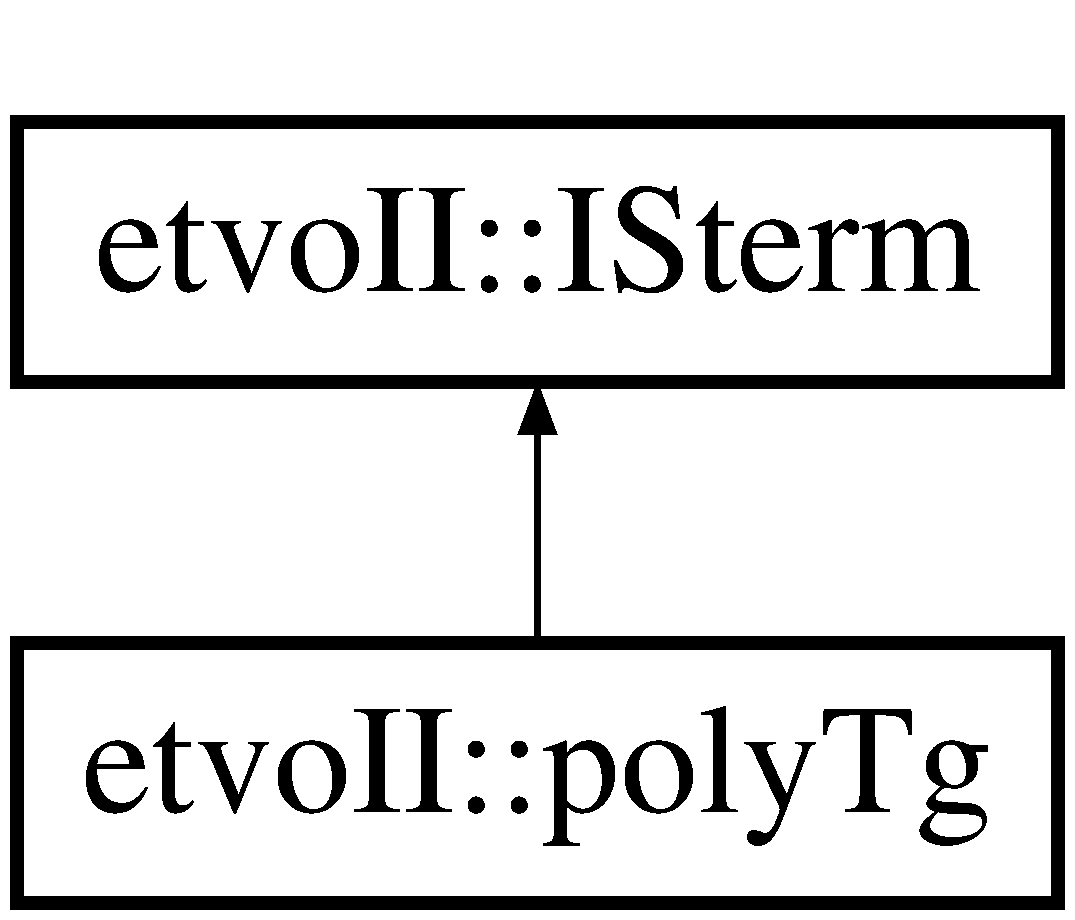
\includegraphics[height=2.000000cm]{classetvo_i_i_1_1poly_tg}
\end{center}
\end{figure}
\subsection*{Public Member Functions}
\begin{DoxyCompactItemize}
\item 
\mbox{\Hypertarget{classetvo_i_i_1_1poly_tg_a51eadd5385e7e950181936fc8465d0bf}\label{classetvo_i_i_1_1poly_tg_a51eadd5385e7e950181936fc8465d0bf}} 
{\bfseries poly\+Tg} (const \mbox{\hyperlink{classetvo_i_i_1_1_tg}{Tg}} \&m)
\item 
\mbox{\Hypertarget{classetvo_i_i_1_1poly_tg_a2f2f176c6c6655791315b4256dcc0428}\label{classetvo_i_i_1_1poly_tg_a2f2f176c6c6655791315b4256dcc0428}} 
{\bfseries poly\+Tg} (bool Top\+NotE)
\item 
\mbox{\Hypertarget{classetvo_i_i_1_1poly_tg_a91a8168c094f2eff996ddb7aacd283fb}\label{classetvo_i_i_1_1poly_tg_a91a8168c094f2eff996ddb7aacd283fb}} 
{\bfseries poly\+Tg} (const std\+::vector$<$ \mbox{\hyperlink{classetvo_i_i_1_1_tg}{Tg}} $>$ \&v)
\item 
\mbox{\Hypertarget{classetvo_i_i_1_1poly_tg_abab3fbca07d31489a6245f8a9baf199a}\label{classetvo_i_i_1_1poly_tg_abab3fbca07d31489a6245f8a9baf199a}} 
\mbox{\hyperlink{classetvo_i_i_1_1poly}{poly}} {\bfseries to\+Poly} () const
\item 
\mbox{\Hypertarget{classetvo_i_i_1_1poly_tg_ac87af312dacba483a82a707a878386f8}\label{classetvo_i_i_1_1poly_tg_ac87af312dacba483a82a707a878386f8}} 
\mbox{\hyperlink{classetvo_i_i_1_1poly_tg}{poly\+Tg}} {\bfseries operator+} (const \mbox{\hyperlink{classetvo_i_i_1_1poly_tg}{poly\+Tg}} \&p) const
\item 
\mbox{\Hypertarget{classetvo_i_i_1_1poly_tg_aa4c184ba112de2a20387e40becd23e74}\label{classetvo_i_i_1_1poly_tg_aa4c184ba112de2a20387e40becd23e74}} 
\mbox{\hyperlink{classetvo_i_i_1_1poly_tg}{poly\+Tg}} {\bfseries oplus} (const \mbox{\hyperlink{classetvo_i_i_1_1poly_tg}{poly\+Tg}} \&p) const
\item 
\mbox{\Hypertarget{classetvo_i_i_1_1poly_tg_af8c8247e5b98c8e25dec5e4e1d0b38f6}\label{classetvo_i_i_1_1poly_tg_af8c8247e5b98c8e25dec5e4e1d0b38f6}} 
\mbox{\hyperlink{classetvo_i_i_1_1poly_tg}{poly\+Tg}} {\bfseries oplus\+CD} (const \mbox{\hyperlink{classetvo_i_i_1_1poly_tg}{poly\+Tg}} \&p) const
\item 
\mbox{\Hypertarget{classetvo_i_i_1_1poly_tg_a770b0005c586ca8c68acf5f90f043342}\label{classetvo_i_i_1_1poly_tg_a770b0005c586ca8c68acf5f90f043342}} 
\mbox{\hyperlink{classetvo_i_i_1_1poly_tg}{poly\+Tg}} {\bfseries operator+} (const \mbox{\hyperlink{classetvo_i_i_1_1_tg}{Tg}} \&m) const
\item 
\mbox{\Hypertarget{classetvo_i_i_1_1poly_tg_af470637282b34e4206028db9dd412f68}\label{classetvo_i_i_1_1poly_tg_af470637282b34e4206028db9dd412f68}} 
void {\bfseries add} (const \mbox{\hyperlink{classetvo_i_i_1_1_tg}{Tg}} \&m)
\item 
\mbox{\Hypertarget{classetvo_i_i_1_1poly_tg_a883331b7b74426c05848660c9922ed10}\label{classetvo_i_i_1_1poly_tg_a883331b7b74426c05848660c9922ed10}} 
\mbox{\hyperlink{classetvo_i_i_1_1poly_tg}{poly\+Tg}} {\bfseries operator$\ast$} (const \mbox{\hyperlink{classetvo_i_i_1_1poly_tg}{poly\+Tg}} \&p) const
\item 
\mbox{\Hypertarget{classetvo_i_i_1_1poly_tg_a69d139c7cd5d77ba977b50d8fd384837}\label{classetvo_i_i_1_1poly_tg_a69d139c7cd5d77ba977b50d8fd384837}} 
\mbox{\hyperlink{classetvo_i_i_1_1poly_tg}{poly\+Tg}} {\bfseries operator$\ast$} (const \mbox{\hyperlink{classetvo_i_i_1_1_tg}{Tg}} \&m) const
\item 
\mbox{\Hypertarget{classetvo_i_i_1_1poly_tg_abff5fda80b1d95eace86bd179e92181e}\label{classetvo_i_i_1_1poly_tg_abff5fda80b1d95eace86bd179e92181e}} 
\mbox{\hyperlink{classetvo_i_i_1_1poly_tg}{poly\+Tg}} {\bfseries otimes} (const \mbox{\hyperlink{classetvo_i_i_1_1poly_tg}{poly\+Tg}} \&p) const
\item 
\mbox{\Hypertarget{classetvo_i_i_1_1poly_tg_ae0ce64acafc33199aadd6dc55d9ddb1a}\label{classetvo_i_i_1_1poly_tg_ae0ce64acafc33199aadd6dc55d9ddb1a}} 
\mbox{\hyperlink{classetvo_i_i_1_1poly_tg}{poly\+Tg}} {\bfseries otimes\+CD} (const \mbox{\hyperlink{classetvo_i_i_1_1poly_tg}{poly\+Tg}} \&p) const
\item 
\mbox{\Hypertarget{classetvo_i_i_1_1poly_tg_a2d27a4aa2c3de8af00757db7d43ec929}\label{classetvo_i_i_1_1poly_tg_a2d27a4aa2c3de8af00757db7d43ec929}} 
\mbox{\hyperlink{classetvo_i_i_1_1poly_tg}{poly\+Tg}} {\bfseries inf} (const \mbox{\hyperlink{classetvo_i_i_1_1poly_tg}{poly\+Tg}} \&p) const
\item 
\mbox{\Hypertarget{classetvo_i_i_1_1poly_tg_a3e12758740b160cb50eeaa8359535900}\label{classetvo_i_i_1_1poly_tg_a3e12758740b160cb50eeaa8359535900}} 
\mbox{\hyperlink{classetvo_i_i_1_1poly_tg}{poly\+Tg}} {\bfseries inf\+CD} (const \mbox{\hyperlink{classetvo_i_i_1_1poly_tg}{poly\+Tg}} \&p) const
\item 
\mbox{\Hypertarget{classetvo_i_i_1_1poly_tg_a4792386c16d07ae5a7af732ff65ea0e5}\label{classetvo_i_i_1_1poly_tg_a4792386c16d07ae5a7af732ff65ea0e5}} 
\mbox{\hyperlink{classetvo_i_i_1_1poly_tg}{poly\+Tg}} {\bfseries lfrac} (const \mbox{\hyperlink{classetvo_i_i_1_1poly_tg}{poly\+Tg}} \&p) const
\item 
\mbox{\Hypertarget{classetvo_i_i_1_1poly_tg_abacccf566a8d120f1055c9896eb42e2d}\label{classetvo_i_i_1_1poly_tg_abacccf566a8d120f1055c9896eb42e2d}} 
\mbox{\hyperlink{classetvo_i_i_1_1poly_tg}{poly\+Tg}} {\bfseries lfrac\+CD} (const \mbox{\hyperlink{classetvo_i_i_1_1poly_tg}{poly\+Tg}} \&p) const
\item 
\mbox{\Hypertarget{classetvo_i_i_1_1poly_tg_aa8ffcea6d42960951b94ca071087a686}\label{classetvo_i_i_1_1poly_tg_aa8ffcea6d42960951b94ca071087a686}} 
\mbox{\hyperlink{classetvo_i_i_1_1poly_tg}{poly\+Tg}} {\bfseries lfrac} (const \mbox{\hyperlink{classetvo_i_i_1_1_tg}{Tg}} \&m) const
\item 
\mbox{\Hypertarget{classetvo_i_i_1_1poly_tg_aad99384f669329aec71d6f407b8972c7}\label{classetvo_i_i_1_1poly_tg_aad99384f669329aec71d6f407b8972c7}} 
\mbox{\hyperlink{classetvo_i_i_1_1poly_tg}{poly\+Tg}} {\bfseries rfrac} (const \mbox{\hyperlink{classetvo_i_i_1_1poly_tg}{poly\+Tg}} \&p) const
\item 
\mbox{\Hypertarget{classetvo_i_i_1_1poly_tg_aae8e6144cc1cef3c1355033b0c16d5ff}\label{classetvo_i_i_1_1poly_tg_aae8e6144cc1cef3c1355033b0c16d5ff}} 
\mbox{\hyperlink{classetvo_i_i_1_1poly_tg}{poly\+Tg}} {\bfseries rfrac\+CD} (const \mbox{\hyperlink{classetvo_i_i_1_1poly_tg}{poly\+Tg}} \&p) const
\item 
\mbox{\Hypertarget{classetvo_i_i_1_1poly_tg_a71171f64c83fd4babcd1cdc6849b9a7d}\label{classetvo_i_i_1_1poly_tg_a71171f64c83fd4babcd1cdc6849b9a7d}} 
\mbox{\hyperlink{classetvo_i_i_1_1poly_tg}{poly\+Tg}} {\bfseries rfrac} (const \mbox{\hyperlink{classetvo_i_i_1_1_tg}{Tg}} \&m) const
\item 
\mbox{\Hypertarget{classetvo_i_i_1_1poly_tg_a102f303739f639174f38cd0b3c132782}\label{classetvo_i_i_1_1poly_tg_a102f303739f639174f38cd0b3c132782}} 
bool {\bfseries operator==} (const \mbox{\hyperlink{classetvo_i_i_1_1poly_tg}{poly\+Tg}} \&) const
\item 
\mbox{\Hypertarget{classetvo_i_i_1_1poly_tg_a341077ff4125249e46589638b24aa869}\label{classetvo_i_i_1_1poly_tg_a341077ff4125249e46589638b24aa869}} 
bool {\bfseries operator!=} (const \mbox{\hyperlink{classetvo_i_i_1_1poly_tg}{poly\+Tg}} \&) const
\item 
\mbox{\Hypertarget{classetvo_i_i_1_1poly_tg_a361269f37b3023584dc85ba2f5139c1f}\label{classetvo_i_i_1_1poly_tg_a361269f37b3023584dc85ba2f5139c1f}} 
bool {\bfseries operator$<$=} (const \mbox{\hyperlink{classetvo_i_i_1_1poly_tg}{poly\+Tg}} \&) const
\item 
\mbox{\Hypertarget{classetvo_i_i_1_1poly_tg_ab593db8253d4aeebd8606710fad3e31e}\label{classetvo_i_i_1_1poly_tg_ab593db8253d4aeebd8606710fad3e31e}} 
bool {\bfseries operator$>$=} (const \mbox{\hyperlink{classetvo_i_i_1_1poly_tg}{poly\+Tg}} \&) const
\item 
\mbox{\Hypertarget{classetvo_i_i_1_1poly_tg_a991fffde5654b2dbe0af41f36b5c9ece}\label{classetvo_i_i_1_1poly_tg_a991fffde5654b2dbe0af41f36b5c9ece}} 
\mbox{\hyperlink{classetvo_i_i_1_1poly_tg}{poly\+Tg}} {\bfseries transient\+Star} (int Tmax) const
\item 
\mbox{\Hypertarget{classetvo_i_i_1_1poly_tg_a3ff16d4529b79874fe5e98c1dc8c88b6}\label{classetvo_i_i_1_1poly_tg_a3ff16d4529b79874fe5e98c1dc8c88b6}} 
\mbox{\hyperlink{classetvo_i_i_1_1_tg}{Tg}} {\bfseries get\+First\+Dif} (const \mbox{\hyperlink{classetvo_i_i_1_1poly_tg}{poly\+Tg}} \&p) const
\item 
\mbox{\Hypertarget{classetvo_i_i_1_1poly_tg_aaa2f904ac840befbca94c5eb5e54d44e}\label{classetvo_i_i_1_1poly_tg_aaa2f904ac840befbca94c5eb5e54d44e}} 
void {\bfseries canon} ()
\item 
\mbox{\Hypertarget{classetvo_i_i_1_1poly_tg_ae1c27b061e6be35f3d2eb37e3dc88ff5}\label{classetvo_i_i_1_1poly_tg_ae1c27b061e6be35f3d2eb37e3dc88ff5}} 
bool {\bfseries is\+Canon} () const
\item 
\mbox{\Hypertarget{classetvo_i_i_1_1poly_tg_a9c83814e41b379df076506277c17f80d}\label{classetvo_i_i_1_1poly_tg_a9c83814e41b379df076506277c17f80d}} 
\mbox{\hyperlink{classetvo_i_i_1_1_tg}{Tg}} {\bfseries operator\mbox{[}$\,$\mbox{]}} (unsigned idx) const
\item 
\mbox{\Hypertarget{classetvo_i_i_1_1poly_tg_a3478ec63c61bd0733feb44d1346abd79}\label{classetvo_i_i_1_1poly_tg_a3478ec63c61bd0733feb44d1346abd79}} 
unsigned int {\bfseries size} () const
\item 
\mbox{\Hypertarget{classetvo_i_i_1_1poly_tg_a16615dcdb674a8563071e167793a5869}\label{classetvo_i_i_1_1poly_tg_a16615dcdb674a8563071e167793a5869}} 
std\+::string {\bfseries to\+String} () const
\item 
\mbox{\Hypertarget{classetvo_i_i_1_1poly_tg_a15eafe0409c5d4a64ff5b4fa79828c0b}\label{classetvo_i_i_1_1poly_tg_a15eafe0409c5d4a64ff5b4fa79828c0b}} 
std\+::string {\bfseries to\+String\+As\+Delta\+Var} () const
\item 
\mbox{\Hypertarget{classetvo_i_i_1_1poly_tg_a541322ec9b45a0d8bd9ccb3ef3869487}\label{classetvo_i_i_1_1poly_tg_a541322ec9b45a0d8bd9ccb3ef3869487}} 
bool {\bfseries isE} () const
\item 
\mbox{\Hypertarget{classetvo_i_i_1_1poly_tg_a59d6ac1f74cb08d2f1076e51fe11491d}\label{classetvo_i_i_1_1poly_tg_a59d6ac1f74cb08d2f1076e51fe11491d}} 
void {\bfseries get\+Max\+Gain} (unsigned int \&mb) const
\item 
\mbox{\Hypertarget{classetvo_i_i_1_1poly_tg_a0d0cdba224e873357e2da17da883c95f}\label{classetvo_i_i_1_1poly_tg_a0d0cdba224e873357e2da17da883c95f}} 
void {\bfseries get\+Lcm\+Gain} (unsigned int \&mb) const
\item 
\mbox{\Hypertarget{classetvo_i_i_1_1poly_tg_a4bfec05f9b189aa2942bdb575b53351d}\label{classetvo_i_i_1_1poly_tg_a4bfec05f9b189aa2942bdb575b53351d}} 
unsigned int {\bfseries get\+Max\+Gain} () const
\item 
\mbox{\Hypertarget{classetvo_i_i_1_1poly_tg_a4de56328e83b821cc0f0041c7b31a405}\label{classetvo_i_i_1_1poly_tg_a4de56328e83b821cc0f0041c7b31a405}} 
unsigned int {\bfseries get\+Lcm\+Gain} () const
\item 
\mbox{\Hypertarget{classetvo_i_i_1_1poly_tg_ad105b9223b1edae79b89c51c73fe98f1}\label{classetvo_i_i_1_1poly_tg_ad105b9223b1edae79b89c51c73fe98f1}} 
unsigned {\bfseries get\+Periodicity} () const
\item 
\mbox{\Hypertarget{classetvo_i_i_1_1poly_tg_a3b606730404c4e887cad5092998b8162}\label{classetvo_i_i_1_1poly_tg_a3b606730404c4e887cad5092998b8162}} 
std\+::vector$<$ \mbox{\hyperlink{classetvo_i_i_1_1_tg}{Tg}} $>$ {\bfseries get\+Terms} () const
\item 
\mbox{\Hypertarget{classetvo_i_i_1_1poly_tg_ab7a34bc66bc3a2dbd76fba0084f9bbdb}\label{classetvo_i_i_1_1poly_tg_ab7a34bc66bc3a2dbd76fba0084f9bbdb}} 
void {\bfseries remove\+Term} (unsigned idx)
\item 
\mbox{\Hypertarget{classetvo_i_i_1_1poly_tg_ab4ff23a26ac7621c410119cf248e2699}\label{classetvo_i_i_1_1poly_tg_ab4ff23a26ac7621c410119cf248e2699}} 
\mbox{\hyperlink{classetvo_i_i_1_1matrix}{matrix}}$<$ \mbox{\hyperlink{classetvo_i_i_1_1poly}{poly}} $>$ {\bfseries get\+Core} (unsigned ratio=1) const
\item 
\mbox{\Hypertarget{classetvo_i_i_1_1poly_tg_aecd2bb7d9b39b30b620ca634acd37bf6}\label{classetvo_i_i_1_1poly_tg_aecd2bb7d9b39b30b620ca634acd37bf6}} 
\mbox{\hyperlink{classetvo_i_i_1_1matrix}{matrix}}$<$ \mbox{\hyperlink{classetvo_i_i_1_1poly}{poly}} $>$ {\bfseries get\+Core\+Max} (unsigned ratio=1) const
\end{DoxyCompactItemize}
\subsection*{Static Public Member Functions}
\begin{DoxyCompactItemize}
\item 
\mbox{\Hypertarget{classetvo_i_i_1_1poly_tg_a2285557904eb669575096b9faae416eb}\label{classetvo_i_i_1_1poly_tg_a2285557904eb669575096b9faae416eb}} 
static \mbox{\hyperlink{classetvo_i_i_1_1poly_tg}{poly\+Tg}} \mbox{\hyperlink{classetvo_i_i_1_1poly_tg_a2285557904eb669575096b9faae416eb}{Epsilon}} ()
\begin{DoxyCompactList}\small\item\em Epsilon, E and Top elements. \end{DoxyCompactList}\item 
\mbox{\Hypertarget{classetvo_i_i_1_1poly_tg_a8b3ec0536f45a8ad3e2375ee0c39e7c4}\label{classetvo_i_i_1_1poly_tg_a8b3ec0536f45a8ad3e2375ee0c39e7c4}} 
static \mbox{\hyperlink{classetvo_i_i_1_1poly_tg}{poly\+Tg}} {\bfseries Top} ()
\item 
\mbox{\Hypertarget{classetvo_i_i_1_1poly_tg_add8eda75a141e5f1434c389493c45dcd}\label{classetvo_i_i_1_1poly_tg_add8eda75a141e5f1434c389493c45dcd}} 
static \mbox{\hyperlink{classetvo_i_i_1_1poly_tg}{poly\+Tg}} {\bfseries E} ()
\item 
\mbox{\Hypertarget{classetvo_i_i_1_1poly_tg_ac3b58c29621a09c45c18bab5e89aabb3}\label{classetvo_i_i_1_1poly_tg_ac3b58c29621a09c45c18bab5e89aabb3}} 
static \mbox{\hyperlink{classetvo_i_i_1_1poly_tg}{poly\+Tg}} {\bfseries to\+Poly\+Tg} (const \mbox{\hyperlink{classetvo_i_i_1_1poly}{poly}} \&p)
\item 
\mbox{\Hypertarget{classetvo_i_i_1_1poly_tg_aec5b4b5f47a5b6be81c77ee25822ade8}\label{classetvo_i_i_1_1poly_tg_aec5b4b5f47a5b6be81c77ee25822ade8}} 
static \mbox{\hyperlink{classetvo_i_i_1_1poly_tg}{poly\+Tg}} {\bfseries otimes} (const \mbox{\hyperlink{classetvo_i_i_1_1_tg}{Tg}} \&m, const \mbox{\hyperlink{classetvo_i_i_1_1poly_tg}{poly\+Tg}} \&p)
\item 
\mbox{\Hypertarget{classetvo_i_i_1_1poly_tg_a82404bc41285950fc405668fbb925a21}\label{classetvo_i_i_1_1poly_tg_a82404bc41285950fc405668fbb925a21}} 
static \mbox{\hyperlink{classetvo_i_i_1_1matrix}{etvo\+I\+I\+::matrix}}$<$ \mbox{\hyperlink{classetvo_i_i_1_1poly}{poly}} $>$ {\bfseries get\+MatN} (unsigned size)
\item 
\mbox{\Hypertarget{classetvo_i_i_1_1poly_tg_a6c9e90cee9ced76c2b6b6e840751280a}\label{classetvo_i_i_1_1poly_tg_a6c9e90cee9ced76c2b6b6e840751280a}} 
static \mbox{\hyperlink{classetvo_i_i_1_1poly_tg}{poly\+Tg}} {\bfseries core\+To\+Poly\+Tg} (const \mbox{\hyperlink{classetvo_i_i_1_1matrix}{matrix}}$<$ \mbox{\hyperlink{classetvo_i_i_1_1poly}{poly}} $>$ \&core)
\end{DoxyCompactItemize}
\subsection*{Additional Inherited Members}


The documentation for this class was generated from the following files\+:\begin{DoxyCompactItemize}
\item 
etvo/series\+Tg/poly\+Tg.\+h\item 
etvo/series\+Tg/poly\+Tg.\+cpp\end{DoxyCompactItemize}

\hypertarget{class_pov_ray_1_1_pov_ray2}{}\section{Pov\+Ray\+:\+:Pov\+Ray2 Class Reference}
\label{class_pov_ray_1_1_pov_ray2}\index{Pov\+Ray\+::\+Pov\+Ray2@{Pov\+Ray\+::\+Pov\+Ray2}}
\subsection*{Classes}
\begin{DoxyCompactItemize}
\item 
class \mbox{\hyperlink{class_pov_ray_1_1_pov_ray2_1_1_color}{Color}}
\item 
class \mbox{\hyperlink{class_pov_ray_1_1_pov_ray2_1_1_point}{Point}}
\end{DoxyCompactItemize}
\subsection*{Public Member Functions}
\begin{DoxyCompactItemize}
\item 
\mbox{\Hypertarget{class_pov_ray_1_1_pov_ray2_a406830b8660f8b663638e088df68f667}\label{class_pov_ray_1_1_pov_ray2_a406830b8660f8b663638e088df68f667}} 
{\bfseries Pov\+Ray2} (const std\+::string \&str)
\item 
\mbox{\Hypertarget{class_pov_ray_1_1_pov_ray2_a6252e0fcb0284511239b958d6055b753}\label{class_pov_ray_1_1_pov_ray2_a6252e0fcb0284511239b958d6055b753}} 
void {\bfseries Repere} ()
\item 
\mbox{\Hypertarget{class_pov_ray_1_1_pov_ray2_a3aca29106ba7b7ea8e10319dc1daff12}\label{class_pov_ray_1_1_pov_ray2_a3aca29106ba7b7ea8e10319dc1daff12}} 
void {\bfseries Fichier\+Pov\+\_\+\+Debut} ()
\item 
\mbox{\Hypertarget{class_pov_ray_1_1_pov_ray2_a86dd8fc3a11b14636660e0e79285bf68}\label{class_pov_ray_1_1_pov_ray2_a86dd8fc3a11b14636660e0e79285bf68}} 
void {\bfseries Fichier\+Pov\+\_\+\+Fin} ()
\item 
\mbox{\Hypertarget{class_pov_ray_1_1_pov_ray2_ae4d0d4637b7c82467f83106251dc5590}\label{class_pov_ray_1_1_pov_ray2_ae4d0d4637b7c82467f83106251dc5590}} 
void {\bfseries Save\+To\+File} ()
\item 
\mbox{\Hypertarget{class_pov_ray_1_1_pov_ray2_a37d75622523e020b273c38a4cfebf0cd}\label{class_pov_ray_1_1_pov_ray2_a37d75622523e020b273c38a4cfebf0cd}} 
void {\bfseries Box} (\mbox{\hyperlink{class_pov_ray_1_1_pov_ray2_1_1_point}{Point}} pA, \mbox{\hyperlink{class_pov_ray_1_1_pov_ray2_1_1_point}{Point}} pB, \mbox{\hyperlink{class_pov_ray_1_1_pov_ray2_1_1_color}{Color}} c)
\item 
\mbox{\Hypertarget{class_pov_ray_1_1_pov_ray2_a953d98ac33a6451d6cf8162d9c107088}\label{class_pov_ray_1_1_pov_ray2_a953d98ac33a6451d6cf8162d9c107088}} 
void {\bfseries Sphere} (\mbox{\hyperlink{class_pov_ray_1_1_pov_ray2_1_1_point}{Point}} centre, float rayon, \mbox{\hyperlink{class_pov_ray_1_1_pov_ray2_1_1_color}{Color}} c)
\item 
\mbox{\Hypertarget{class_pov_ray_1_1_pov_ray2_ac9831468bc6d2d197682845c7ee6c7f7}\label{class_pov_ray_1_1_pov_ray2_ac9831468bc6d2d197682845c7ee6c7f7}} 
void {\bfseries Cylindre} (\mbox{\hyperlink{class_pov_ray_1_1_pov_ray2_1_1_point}{Point}} pA, \mbox{\hyperlink{class_pov_ray_1_1_pov_ray2_1_1_point}{Point}} pB, float rayon, \mbox{\hyperlink{class_pov_ray_1_1_pov_ray2_1_1_color}{Color}} c)
\item 
\mbox{\Hypertarget{class_pov_ray_1_1_pov_ray2_a1f61a4895abc1fd884e2fdf9fbcff3c2}\label{class_pov_ray_1_1_pov_ray2_a1f61a4895abc1fd884e2fdf9fbcff3c2}} 
void {\bfseries Face\+XY} (\mbox{\hyperlink{class_pov_ray_1_1_pov_ray2_1_1_point}{Point}} pA, \mbox{\hyperlink{class_pov_ray_1_1_pov_ray2_1_1_point}{Point}} pB)
\item 
\mbox{\Hypertarget{class_pov_ray_1_1_pov_ray2_a9297aff14816d16ef1fa58e392280779}\label{class_pov_ray_1_1_pov_ray2_a9297aff14816d16ef1fa58e392280779}} 
void {\bfseries FaceZ} (\mbox{\hyperlink{class_pov_ray_1_1_pov_ray2_1_1_point}{Point}} pA, \mbox{\hyperlink{class_pov_ray_1_1_pov_ray2_1_1_point}{Point}} pB)
\end{DoxyCompactItemize}
\subsection*{Public Attributes}
\begin{DoxyCompactItemize}
\item 
\mbox{\Hypertarget{class_pov_ray_1_1_pov_ray2_abba09dc6793e4ac70e75b30f5b9b5082}\label{class_pov_ray_1_1_pov_ray2_abba09dc6793e4ac70e75b30f5b9b5082}} 
\mbox{\hyperlink{class_pov_ray_1_1_pov_ray2_1_1_point}{Point}} {\bfseries Position\+Camera}
\item 
\mbox{\Hypertarget{class_pov_ray_1_1_pov_ray2_a219dab2e4a54b7ff61727246837458fa}\label{class_pov_ray_1_1_pov_ray2_a219dab2e4a54b7ff61727246837458fa}} 
\mbox{\hyperlink{class_pov_ray_1_1_pov_ray2_1_1_point}{Point}} {\bfseries Camera\+Look\+At}
\item 
\mbox{\Hypertarget{class_pov_ray_1_1_pov_ray2_ab8c81f8038e987667f05ebfea64d29b9}\label{class_pov_ray_1_1_pov_ray2_ab8c81f8038e987667f05ebfea64d29b9}} 
\mbox{\hyperlink{class_pov_ray_1_1_pov_ray2_1_1_color}{Color}} {\bfseries C\+Surface}
\item 
\mbox{\Hypertarget{class_pov_ray_1_1_pov_ray2_aac21b14144097da2b288dd35ffca5885}\label{class_pov_ray_1_1_pov_ray2_aac21b14144097da2b288dd35ffca5885}} 
int {\bfseries xmin}
\item 
\mbox{\Hypertarget{class_pov_ray_1_1_pov_ray2_a2a7b42fbe8d38ecc0b4071205e0c5e20}\label{class_pov_ray_1_1_pov_ray2_a2a7b42fbe8d38ecc0b4071205e0c5e20}} 
int {\bfseries ymax}
\item 
\mbox{\Hypertarget{class_pov_ray_1_1_pov_ray2_aa5ad3e488bc8153cc45ba918409dbf96}\label{class_pov_ray_1_1_pov_ray2_aa5ad3e488bc8153cc45ba918409dbf96}} 
int {\bfseries zmin}
\item 
\mbox{\Hypertarget{class_pov_ray_1_1_pov_ray2_a342e45e1769ece5a245fd647c77060ce}\label{class_pov_ray_1_1_pov_ray2_a342e45e1769ece5a245fd647c77060ce}} 
int {\bfseries xmax}
\item 
\mbox{\Hypertarget{class_pov_ray_1_1_pov_ray2_a715ef2f3a63a842780f08c3bafe275dc}\label{class_pov_ray_1_1_pov_ray2_a715ef2f3a63a842780f08c3bafe275dc}} 
int {\bfseries zmax}
\item 
\mbox{\Hypertarget{class_pov_ray_1_1_pov_ray2_a5132ba86a9dccd58f6965a19b2491ffc}\label{class_pov_ray_1_1_pov_ray2_a5132ba86a9dccd58f6965a19b2491ffc}} 
int {\bfseries ymin}
\item 
\mbox{\Hypertarget{class_pov_ray_1_1_pov_ray2_a9a1db6d7b3ac0907ce91a73958458d4f}\label{class_pov_ray_1_1_pov_ray2_a9a1db6d7b3ac0907ce91a73958458d4f}} 
std\+::string {\bfseries nom\+Fichier\+Dfx}
\item 
\mbox{\Hypertarget{class_pov_ray_1_1_pov_ray2_a262172e2cbfcaeff82b88d054673e9d6}\label{class_pov_ray_1_1_pov_ray2_a262172e2cbfcaeff82b88d054673e9d6}} 
std\+::strstream {\bfseries ss}
\end{DoxyCompactItemize}


The documentation for this class was generated from the following files\+:\begin{DoxyCompactItemize}
\item 
etvo/grafic/Pov\+Ray2.\+h\item 
etvo/grafic/Pov\+Ray2.\+cpp\end{DoxyCompactItemize}

\hypertarget{classetvo_i_i_1_1rand_gen}{}\section{etvo\+II\+:\+:rand\+Gen Class Reference}
\label{classetvo_i_i_1_1rand_gen}\index{etvo\+I\+I\+::rand\+Gen@{etvo\+I\+I\+::rand\+Gen}}
\subsection*{Static Public Member Functions}
\begin{DoxyCompactItemize}
\item 
\mbox{\Hypertarget{classetvo_i_i_1_1rand_gen_a4363a2d9a3bb53dff78264ad3e0123dc}\label{classetvo_i_i_1_1rand_gen_a4363a2d9a3bb53dff78264ad3e0123dc}} 
static int {\bfseries uni\+\_\+int} (int mini, int maxi)
\item 
\mbox{\Hypertarget{classetvo_i_i_1_1rand_gen_a4337921dc310b89c2473d3e2a0d7fd65}\label{classetvo_i_i_1_1rand_gen_a4337921dc310b89c2473d3e2a0d7fd65}} 
static int {\bfseries norm\+\_\+int} (int mini, int maxi)
\item 
\mbox{\Hypertarget{classetvo_i_i_1_1rand_gen_abe5be8388f069c984ea0a416dd2f6874}\label{classetvo_i_i_1_1rand_gen_abe5be8388f069c984ea0a416dd2f6874}} 
static \mbox{\hyperlink{classetvo_i_i_1_1poly}{etvo\+I\+I\+::poly}} {\bfseries Rand\+\_\+poly} (unsigned nb\+Terms, const \mbox{\hyperlink{classetvo_i_i_1_1gd}{etvo\+I\+I\+::gd}} \&offset, int max\+Gap=5)
\item 
\mbox{\Hypertarget{classetvo_i_i_1_1rand_gen_a4eaa8f9c89f80bc0b1706733657af7eb}\label{classetvo_i_i_1_1rand_gen_a4eaa8f9c89f80bc0b1706733657af7eb}} 
static \mbox{\hyperlink{classetvo_i_i_1_1poly}{etvo\+I\+I\+::poly}} {\bfseries Rand\+\_\+poly} (unsigned nb\+Terms)
\item 
\mbox{\Hypertarget{classetvo_i_i_1_1rand_gen_aa70969b36e5cc6600959bcf10fae5de9}\label{classetvo_i_i_1_1rand_gen_aa70969b36e5cc6600959bcf10fae5de9}} 
static \mbox{\hyperlink{classetvo_i_i_1_1series}{etvo\+I\+I\+::series}} {\bfseries Rand\+\_\+series} (unsigned n\+Terms, const \mbox{\hyperlink{classetvo_i_i_1_1gd}{etvo\+I\+I\+::gd}} \&slopeR=\mbox{\hyperlink{classetvo_i_i_1_1gd}{gd}}(5, 6), const \mbox{\hyperlink{classetvo_i_i_1_1gd}{etvo\+I\+I\+::gd}} \&offset=\mbox{\hyperlink{classetvo_i_i_1_1gd}{etvo\+I\+I\+::gd}}(0, 0), int max\+Gap=5)
\item 
\mbox{\Hypertarget{classetvo_i_i_1_1rand_gen_a15d6c9cab96f643813f37fa71b413ace}\label{classetvo_i_i_1_1rand_gen_a15d6c9cab96f643813f37fa71b413ace}} 
static \mbox{\hyperlink{classetvo_i_i_1_1g_ng}{etvo\+I\+I\+::g\+Ng}} {\bfseries Rand\+\_\+g\+Ng} ()
\item 
\mbox{\Hypertarget{classetvo_i_i_1_1rand_gen_a6765c9abd785a0f192d62943556ab7b6}\label{classetvo_i_i_1_1rand_gen_a6765c9abd785a0f192d62943556ab7b6}} 
static \mbox{\hyperlink{classetvo_i_i_1_1d_dd}{etvo\+I\+I\+::d\+Dd}} {\bfseries Rand\+\_\+d\+Dd} ()
\item 
\mbox{\Hypertarget{classetvo_i_i_1_1rand_gen_a80f77da93edc9515d518c539f1cc468c}\label{classetvo_i_i_1_1rand_gen_a80f77da93edc9515d518c539f1cc468c}} 
static \mbox{\hyperlink{classetvo_i_i_1_1_fper}{etvo\+I\+I\+::\+Fper}} {\bfseries Rand\+\_\+\+Fper\+\_\+fixed\+Per} (int range\+Y0, int dP, int codP)
\item 
\mbox{\Hypertarget{classetvo_i_i_1_1rand_gen_a04868fddf9b38dafb1840cfe02a11416}\label{classetvo_i_i_1_1rand_gen_a04868fddf9b38dafb1840cfe02a11416}} 
static \mbox{\hyperlink{classetvo_i_i_1_1_fper}{etvo\+I\+I\+::\+Fper}} {\bfseries Rand\+\_\+\+Fper\+\_\+fixed\+Per\+\_\+and\+\_\+\+Y0} (int Y0, int dP, int codP)
\item 
\mbox{\Hypertarget{classetvo_i_i_1_1rand_gen_ab3e1bdffd58ebfffac344243d78a6038}\label{classetvo_i_i_1_1rand_gen_ab3e1bdffd58ebfffac344243d78a6038}} 
static \mbox{\hyperlink{classetvo_i_i_1_1_fminp}{etvo\+I\+I\+::\+Fminp}} {\bfseries Rand\+\_\+\+Fminp\+\_\+fixed\+Per} (int range\+Y0, int dP, int codP)
\item 
\mbox{\Hypertarget{classetvo_i_i_1_1rand_gen_a0752ba7864ee9adde6340a6def1d4379}\label{classetvo_i_i_1_1rand_gen_a0752ba7864ee9adde6340a6def1d4379}} 
static \mbox{\hyperlink{classetvo_i_i_1_1_fminp}{etvo\+I\+I\+::\+Fminp}} {\bfseries Rand\+\_\+\+Fminp\+\_\+fixed\+Per\+\_\+and\+\_\+\+Y0} (int Y0, int dP, int codP)
\item 
\mbox{\Hypertarget{classetvo_i_i_1_1rand_gen_ae27f1bbeb708fda85e6e4a23a3905401}\label{classetvo_i_i_1_1rand_gen_ae27f1bbeb708fda85e6e4a23a3905401}} 
static \mbox{\hyperlink{classetvo_i_i_1_1_fmaxp}{etvo\+I\+I\+::\+Fmaxp}} {\bfseries Rand\+\_\+\+Fmaxp\+\_\+fixed\+Per} (int range\+Y0, int dP, int codP)
\item 
\mbox{\Hypertarget{classetvo_i_i_1_1rand_gen_a95a221a53fe9084bde09080d9d9ceffe}\label{classetvo_i_i_1_1rand_gen_a95a221a53fe9084bde09080d9d9ceffe}} 
static \mbox{\hyperlink{classetvo_i_i_1_1_fmaxp}{etvo\+I\+I\+::\+Fmaxp}} {\bfseries Rand\+\_\+\+Fmaxp\+\_\+fixed\+Per\+\_\+and\+\_\+\+Y0} (int Y0, int dP, int codP)
\item 
\mbox{\Hypertarget{classetvo_i_i_1_1rand_gen_a74c0a6e99d5aaed5b42008064d2f24da}\label{classetvo_i_i_1_1rand_gen_a74c0a6e99d5aaed5b42008064d2f24da}} 
static \mbox{\hyperlink{classetvo_i_i_1_1_e__op}{etvo\+I\+I\+::\+E\+\_\+op}} {\bfseries Rand\+\_\+\+Eop\+\_\+fixedG} (unsigned Me, unsigned Be)
\item 
\mbox{\Hypertarget{classetvo_i_i_1_1rand_gen_aa7ad68ff6717ea680cde9bcd122121bf}\label{classetvo_i_i_1_1rand_gen_aa7ad68ff6717ea680cde9bcd122121bf}} 
static \mbox{\hyperlink{classetvo_i_i_1_1_e__op}{etvo\+I\+I\+::\+E\+\_\+op}} {\bfseries Rand\+\_\+\+Eop\+\_\+fixedG} (unsigned Me, unsigned Be, int g0)
\item 
\mbox{\Hypertarget{classetvo_i_i_1_1rand_gen_acec699b0a1f209940d36ff7c3d8fa869}\label{classetvo_i_i_1_1rand_gen_acec699b0a1f209940d36ff7c3d8fa869}} 
static \mbox{\hyperlink{classetvo_i_i_1_1_e__op}{etvo\+I\+I\+::\+E\+\_\+op}} {\bfseries Rand\+\_\+\+Eop} (unsigned Me, unsigned Be)
\item 
\mbox{\Hypertarget{classetvo_i_i_1_1rand_gen_a56a94a200990e66c84fdc04397fd7c1b}\label{classetvo_i_i_1_1rand_gen_a56a94a200990e66c84fdc04397fd7c1b}} 
static \mbox{\hyperlink{classetvo_i_i_1_1_t__op}{etvo\+I\+I\+::\+T\+\_\+op}} {\bfseries Rand\+\_\+\+Top\+\_\+fixedG} (unsigned M\+Be)
\item 
\mbox{\Hypertarget{classetvo_i_i_1_1rand_gen_ad3d9e1456541f914aa65a2b2ad51dfeb}\label{classetvo_i_i_1_1rand_gen_ad3d9e1456541f914aa65a2b2ad51dfeb}} 
static \mbox{\hyperlink{classetvo_i_i_1_1_t__op}{etvo\+I\+I\+::\+T\+\_\+op}} {\bfseries Rand\+\_\+\+Top\+\_\+fixedG} (unsigned M\+Be, int t0)
\item 
\mbox{\Hypertarget{classetvo_i_i_1_1rand_gen_aea3a14151abeca9252b2b8f61fbafb16}\label{classetvo_i_i_1_1rand_gen_aea3a14151abeca9252b2b8f61fbafb16}} 
static \mbox{\hyperlink{classetvo_i_i_1_1_t__op}{etvo\+I\+I\+::\+T\+\_\+op}} {\bfseries Rand\+\_\+\+Top} (unsigned M\+Be)
\item 
\mbox{\Hypertarget{classetvo_i_i_1_1rand_gen_adae5598bf2555baff236ee0a79f188a2}\label{classetvo_i_i_1_1rand_gen_adae5598bf2555baff236ee0a79f188a2}} 
static \mbox{\hyperlink{classetvo_i_i_1_1_ed}{etvo\+I\+I\+::\+Ed}} {\bfseries Rand\+\_\+\+Ed} (unsigned Me, unsigned Be)
\item 
\mbox{\Hypertarget{classetvo_i_i_1_1rand_gen_a8310b89d802701510e20287bc75ab544}\label{classetvo_i_i_1_1rand_gen_a8310b89d802701510e20287bc75ab544}} 
static \mbox{\hyperlink{classetvo_i_i_1_1_ed}{etvo\+I\+I\+::\+Ed}} {\bfseries Rand\+\_\+\+Ed} (unsigned Me, unsigned Be, int g, int d)
\item 
\mbox{\Hypertarget{classetvo_i_i_1_1rand_gen_ae89919ba9d282c6e9017ff12201f5be8}\label{classetvo_i_i_1_1rand_gen_ae89919ba9d282c6e9017ff12201f5be8}} 
static \mbox{\hyperlink{classetvo_i_i_1_1_ed}{etvo\+I\+I\+::\+Ed}} {\bfseries Rand\+\_\+\+Ed\+\_\+fixedG} (unsigned Me, unsigned Be)
\item 
\mbox{\Hypertarget{classetvo_i_i_1_1rand_gen_aa5f7ee429f8ac5603d05eb7e9b9e76ce}\label{classetvo_i_i_1_1rand_gen_aa5f7ee429f8ac5603d05eb7e9b9e76ce}} 
static \mbox{\hyperlink{classetvo_i_i_1_1_ed}{etvo\+I\+I\+::\+Ed}} {\bfseries Rand\+\_\+\+Ed\+\_\+fixedG} (unsigned Me, unsigned Be, int g, int d)
\item 
\mbox{\Hypertarget{classetvo_i_i_1_1rand_gen_ac1971471dd5fd1dfb701a793fa85b0f9}\label{classetvo_i_i_1_1rand_gen_ac1971471dd5fd1dfb701a793fa85b0f9}} 
static \mbox{\hyperlink{classetvo_i_i_1_1_tg}{etvo\+I\+I\+::\+Tg}} {\bfseries Rand\+\_\+\+Tg} (unsigned M\+Be)
\item 
\mbox{\Hypertarget{classetvo_i_i_1_1rand_gen_aedfca967a86433dc52ae3369f37dddbc}\label{classetvo_i_i_1_1rand_gen_aedfca967a86433dc52ae3369f37dddbc}} 
static \mbox{\hyperlink{classetvo_i_i_1_1_tg}{etvo\+I\+I\+::\+Tg}} {\bfseries Rand\+\_\+\+Tg} (unsigned M\+Be, int g, int d)
\item 
\mbox{\Hypertarget{classetvo_i_i_1_1rand_gen_a4cee5b998d862ddea1cf0662be8729a2}\label{classetvo_i_i_1_1rand_gen_a4cee5b998d862ddea1cf0662be8729a2}} 
static \mbox{\hyperlink{classetvo_i_i_1_1_tg}{etvo\+I\+I\+::\+Tg}} {\bfseries Rand\+\_\+\+Tg\+\_\+fixedG} (unsigned M\+Be)
\item 
\mbox{\Hypertarget{classetvo_i_i_1_1rand_gen_a037c88b962068630eb83cd520793a192}\label{classetvo_i_i_1_1rand_gen_a037c88b962068630eb83cd520793a192}} 
static \mbox{\hyperlink{classetvo_i_i_1_1_tg}{etvo\+I\+I\+::\+Tg}} {\bfseries Rand\+\_\+\+Tg\+\_\+fixedG} (unsigned M\+Be, int g, int d)
\item 
\mbox{\Hypertarget{classetvo_i_i_1_1rand_gen_a61e9c09c412bb5379613875156ab2eda}\label{classetvo_i_i_1_1rand_gen_a61e9c09c412bb5379613875156ab2eda}} 
static \mbox{\hyperlink{classetvo_i_i_1_1poly_ed}{etvo\+I\+I\+::poly\+Ed}} {\bfseries Rand\+\_\+poly\+Ed\+\_\+fixedG} (unsigned Me, unsigned Be, unsigned nb\+Terms, int max\+Gap=5)
\item 
\mbox{\Hypertarget{classetvo_i_i_1_1rand_gen_a33980f4ee6a8365039ad02716df018a9}\label{classetvo_i_i_1_1rand_gen_a33980f4ee6a8365039ad02716df018a9}} 
static \mbox{\hyperlink{classetvo_i_i_1_1poly_ed}{etvo\+I\+I\+::poly\+Ed}} {\bfseries Rand\+\_\+poly\+Ed\+\_\+fixedG} (const \mbox{\hyperlink{classetvo_i_i_1_1gd}{etvo\+I\+I\+::gd}} \&offset, unsigned Me, unsigned Be, unsigned nb\+Terms, int max\+Gap=5)
\item 
\mbox{\Hypertarget{classetvo_i_i_1_1rand_gen_a90303733bca6a7a59af7b98b492ff77a}\label{classetvo_i_i_1_1rand_gen_a90303733bca6a7a59af7b98b492ff77a}} 
static \mbox{\hyperlink{classetvo_i_i_1_1poly_ed}{etvo\+I\+I\+::poly\+Ed}} {\bfseries Rand\+\_\+poly\+Ed} (unsigned M, unsigned B, unsigned nb\+Terms, int max\+Gap=5)
\item 
\mbox{\Hypertarget{classetvo_i_i_1_1rand_gen_a29d2870f8afaa1514813338b737fa04a}\label{classetvo_i_i_1_1rand_gen_a29d2870f8afaa1514813338b737fa04a}} 
static \mbox{\hyperlink{classetvo_i_i_1_1series_ed}{etvo\+I\+I\+::series\+Ed}} {\bfseries Rand\+\_\+series\+Ed\+\_\+fixedG} (unsigned Me, unsigned Be, unsigned nb\+Terms, const \mbox{\hyperlink{classetvo_i_i_1_1gd}{etvo\+I\+I\+::gd}} \&off=\mbox{\hyperlink{classetvo_i_i_1_1gd}{etvo\+I\+I\+::gd}}(0, 0))
\item 
\mbox{\Hypertarget{classetvo_i_i_1_1rand_gen_a8be2a462220c03d85e5ac4d5fca2ef24}\label{classetvo_i_i_1_1rand_gen_a8be2a462220c03d85e5ac4d5fca2ef24}} 
static \mbox{\hyperlink{classetvo_i_i_1_1series_ed}{etvo\+I\+I\+::series\+Ed}} {\bfseries Rand\+\_\+series\+Ed\+\_\+fixed\+G\+\_\+fixed\+Slope} (unsigned Me, unsigned Be, const \mbox{\hyperlink{classetvo_i_i_1_1gd}{etvo\+I\+I\+::gd}} \&r\+Slope, unsigned nb\+Terms, const \mbox{\hyperlink{classetvo_i_i_1_1gd}{etvo\+I\+I\+::gd}} \&off=\mbox{\hyperlink{classetvo_i_i_1_1gd}{etvo\+I\+I\+::gd}}(0, 0))
\item 
\mbox{\Hypertarget{classetvo_i_i_1_1rand_gen_a8c466846aad58c75d33e59dfe3402a69}\label{classetvo_i_i_1_1rand_gen_a8c466846aad58c75d33e59dfe3402a69}} 
static \mbox{\hyperlink{classetvo_i_i_1_1series_ed}{etvo\+I\+I\+::series\+Ed}} {\bfseries Rand\+\_\+series\+Ed} (unsigned Me, unsigned Be, unsigned nb\+Terms, const \mbox{\hyperlink{classetvo_i_i_1_1gd}{etvo\+I\+I\+::gd}} \&off=\mbox{\hyperlink{classetvo_i_i_1_1gd}{etvo\+I\+I\+::gd}}(0, 0))
\item 
\mbox{\Hypertarget{classetvo_i_i_1_1rand_gen_a46f376d7abf5aecd53e0c57ff937aee6}\label{classetvo_i_i_1_1rand_gen_a46f376d7abf5aecd53e0c57ff937aee6}} 
static \mbox{\hyperlink{classetvo_i_i_1_1poly_tg}{etvo\+I\+I\+::poly\+Tg}} {\bfseries Rand\+\_\+poly\+Tg\+\_\+fixedG} (unsigned M\+Be, unsigned nb\+Terms, int max\+Gap=5)
\item 
\mbox{\Hypertarget{classetvo_i_i_1_1rand_gen_afceec5373e9dad39ee2651057400aaf3}\label{classetvo_i_i_1_1rand_gen_afceec5373e9dad39ee2651057400aaf3}} 
static \mbox{\hyperlink{classetvo_i_i_1_1poly_tg}{etvo\+I\+I\+::poly\+Tg}} {\bfseries Rand\+\_\+poly\+Tg} (unsigned MB, unsigned nb\+Terms, int max\+Gap=5)
\item 
\mbox{\Hypertarget{classetvo_i_i_1_1rand_gen_adf85b7a4f41ff0c634043692ded65b91}\label{classetvo_i_i_1_1rand_gen_adf85b7a4f41ff0c634043692ded65b91}} 
static \mbox{\hyperlink{classetvo_i_i_1_1poly_tg}{etvo\+I\+I\+::poly\+Tg}} {\bfseries Rand\+\_\+poly\+Tg\+\_\+fixedG} (const \mbox{\hyperlink{classetvo_i_i_1_1gd}{etvo\+I\+I\+::gd}} \&offset, unsigned MB, unsigned nb\+Terms, int max\+Gap=5)
\end{DoxyCompactItemize}


The documentation for this class was generated from the following files\+:\begin{DoxyCompactItemize}
\item 
etvo/factory/rand\+Gen.\+h\item 
etvo/factory/rand\+Gen.\+cpp\end{DoxyCompactItemize}

\hypertarget{classmmgd_1_1serie}{}\section{mmgd\+:\+:serie Class Reference}
\label{classmmgd_1_1serie}\index{mmgd\+::serie@{mmgd\+::serie}}
Inheritance diagram for mmgd\+:\+:serie\+:\begin{figure}[H]
\begin{center}
\leavevmode
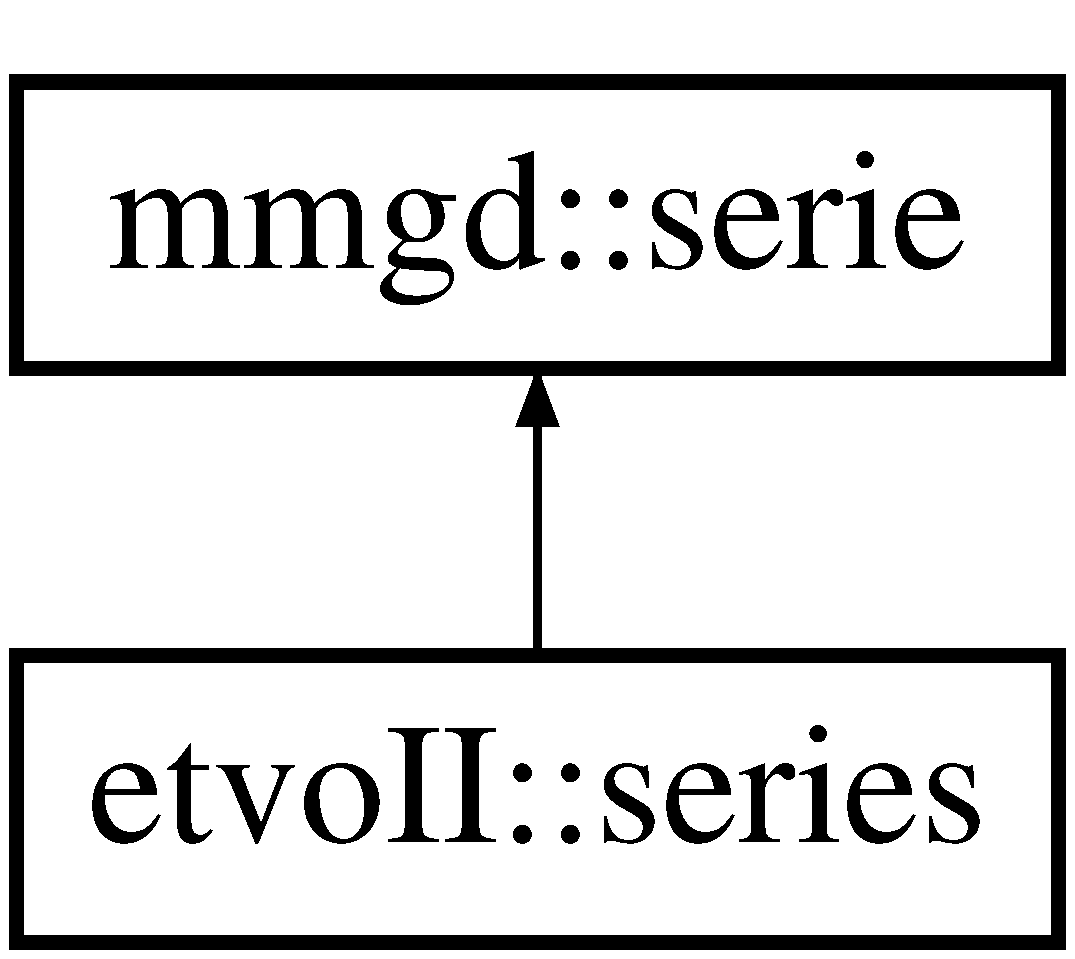
\includegraphics[height=2.000000cm]{classmmgd_1_1serie}
\end{center}
\end{figure}
\subsection*{Public Member Functions}
\begin{DoxyCompactItemize}
\item 
\mbox{\Hypertarget{classmmgd_1_1serie_aaa97a51daa7e06a231be806a84bd6073}\label{classmmgd_1_1serie_aaa97a51daa7e06a231be806a84bd6073}} 
{\bfseries serie} (const \mbox{\hyperlink{classmmgd_1_1serie}{serie}} \&)
\item 
\mbox{\Hypertarget{classmmgd_1_1serie_a2e5e176ba9944ac572e1999018e44886}\label{classmmgd_1_1serie_a2e5e176ba9944ac572e1999018e44886}} 
{\bfseries serie} (const \mbox{\hyperlink{classmmgd_1_1poly}{poly}} \&p1, const \mbox{\hyperlink{classmmgd_1_1poly}{poly}} \&q1, \mbox{\hyperlink{classmmgd_1_1gd}{gd}} \&r1)
\item 
\mbox{\Hypertarget{classmmgd_1_1serie_a4725a58c8ea4de37d2cdd88dd5b4c914}\label{classmmgd_1_1serie_a4725a58c8ea4de37d2cdd88dd5b4c914}} 
{\bfseries serie} (\mbox{\hyperlink{classmmgd_1_1poly}{poly}} \&p)
\item 
\mbox{\Hypertarget{classmmgd_1_1serie_a33e8a0a46077473352724801e10b3cf6}\label{classmmgd_1_1serie_a33e8a0a46077473352724801e10b3cf6}} 
{\bfseries serie} (\mbox{\hyperlink{classmmgd_1_1gd}{gd}} \&gd1)
\item 
\mbox{\Hypertarget{classmmgd_1_1serie_af3813bfd7099de4e1b0493dc310bd3fc}\label{classmmgd_1_1serie_af3813bfd7099de4e1b0493dc310bd3fc}} 
{\bfseries serie} (unsigned int np1, unsigned int nq1, \mbox{\hyperlink{classmmgd_1_1gd}{gd}} $\ast$p1, \mbox{\hyperlink{classmmgd_1_1gd}{gd}} $\ast$q1, \mbox{\hyperlink{classmmgd_1_1gd}{gd}} \&r1)
\item 
\mbox{\Hypertarget{classmmgd_1_1serie_a38fbdc0f684b65730903fcc2a75c2e06}\label{classmmgd_1_1serie_a38fbdc0f684b65730903fcc2a75c2e06}} 
\mbox{\hyperlink{classmmgd_1_1poly}{poly}} \& {\bfseries getp} (void)
\item 
\mbox{\Hypertarget{classmmgd_1_1serie_a67c4d214b2e02022f54ff8ff63e657f9}\label{classmmgd_1_1serie_a67c4d214b2e02022f54ff8ff63e657f9}} 
\mbox{\hyperlink{classmmgd_1_1poly}{poly}} \& {\bfseries getq} (void)
\item 
\mbox{\Hypertarget{classmmgd_1_1serie_a0650364b2ecc501864fa6e684053aa57}\label{classmmgd_1_1serie_a0650364b2ecc501864fa6e684053aa57}} 
\mbox{\hyperlink{classmmgd_1_1gd}{gd}} \& {\bfseries getr} (void)
\item 
\mbox{\Hypertarget{classmmgd_1_1serie_a066f2b3c24ff28b1b771040c7e01166e}\label{classmmgd_1_1serie_a066f2b3c24ff28b1b771040c7e01166e}} 
\mbox{\hyperlink{classmmgd_1_1serie}{serie}} \& {\bfseries operator=} (const \mbox{\hyperlink{classmmgd_1_1serie}{serie}} \&serie1)
\item 
\mbox{\Hypertarget{classmmgd_1_1serie_a2f14a188cfab4354429d9f0f87a82e58}\label{classmmgd_1_1serie_a2f14a188cfab4354429d9f0f87a82e58}} 
\mbox{\hyperlink{classmmgd_1_1serie}{serie}} \& {\bfseries operator=} (const \mbox{\hyperlink{classmmgd_1_1gd}{gd}} \&gd1)
\item 
\mbox{\Hypertarget{classmmgd_1_1serie_a21cca4fee933ae71f605215b13a612ae}\label{classmmgd_1_1serie_a21cca4fee933ae71f605215b13a612ae}} 
\mbox{\hyperlink{classmmgd_1_1serie}{serie}} \& {\bfseries operator=} (const \mbox{\hyperlink{classmmgd_1_1poly}{poly}} \&p1)
\item 
\mbox{\Hypertarget{classmmgd_1_1serie_a3ec7bfdba701b17e56c055e0a9486b6e}\label{classmmgd_1_1serie_a3ec7bfdba701b17e56c055e0a9486b6e}} 
void {\bfseries init} (\mbox{\hyperlink{classmmgd_1_1poly}{poly}} \&p1, \mbox{\hyperlink{classmmgd_1_1poly}{poly}} \&q1, \mbox{\hyperlink{classmmgd_1_1gd}{gd}} \&r1)
\item 
\mbox{\Hypertarget{classmmgd_1_1serie_ac01a3e0aea64486c264500293c6313d6}\label{classmmgd_1_1serie_ac01a3e0aea64486c264500293c6313d6}} 
void {\bfseries init} (unsigned int, unsigned int, \mbox{\hyperlink{classmmgd_1_1gd}{gd}} $\ast$, \mbox{\hyperlink{classmmgd_1_1gd}{gd}} $\ast$, \mbox{\hyperlink{classmmgd_1_1gd}{gd}} \&)
\item 
\mbox{\Hypertarget{classmmgd_1_1serie_a15d0c0636e2cf65ee8af81def95d0242}\label{classmmgd_1_1serie_a15d0c0636e2cf65ee8af81def95d0242}} 
void {\bfseries init} (\mbox{\hyperlink{classmmgd_1_1gd}{gd}} \&pgd1, \mbox{\hyperlink{classmmgd_1_1gd}{gd}} \&qgd1, \mbox{\hyperlink{classmmgd_1_1gd}{gd}} \&r1)
\item 
\mbox{\Hypertarget{classmmgd_1_1serie_a1485f36c62d4a6d3c5861c12219d28e2}\label{classmmgd_1_1serie_a1485f36c62d4a6d3c5861c12219d28e2}} 
void {\bfseries init} (\mbox{\hyperlink{classmmgd_1_1poly}{poly}} \&p1, \mbox{\hyperlink{classmmgd_1_1gd}{gd}} \&qgd1, \mbox{\hyperlink{classmmgd_1_1gd}{gd}} \&r1)
\item 
\mbox{\Hypertarget{classmmgd_1_1serie_a63454c770de7d4ee7f0216c21183574b}\label{classmmgd_1_1serie_a63454c770de7d4ee7f0216c21183574b}} 
void {\bfseries init} (\mbox{\hyperlink{classmmgd_1_1gd}{gd}} \&pgd1, \mbox{\hyperlink{classmmgd_1_1poly}{poly}} \&q1, \mbox{\hyperlink{classmmgd_1_1gd}{gd}} \&r1)
\item 
\mbox{\Hypertarget{classmmgd_1_1serie_a37939ffcb52ec8f82a45c54e34b8d3fe}\label{classmmgd_1_1serie_a37939ffcb52ec8f82a45c54e34b8d3fe}} 
void {\bfseries canon} ()
\item 
\mbox{\Hypertarget{classmmgd_1_1serie_a1d28f3f8c8f4a4f5e7b3cf17102faf25}\label{classmmgd_1_1serie_a1d28f3f8c8f4a4f5e7b3cf17102faf25}} 
int {\bfseries operator==} (\mbox{\hyperlink{classmmgd_1_1serie}{serie}} \&)
\end{DoxyCompactItemize}
\subsection*{Static Public Attributes}
\begin{DoxyCompactItemize}
\item 
\mbox{\Hypertarget{classmmgd_1_1serie_a5b098609ed451a16502695db01e95543}\label{classmmgd_1_1serie_a5b098609ed451a16502695db01e95543}} 
static \mbox{\hyperlink{classmmgd_1_1serie}{serie}} {\bfseries eps}
\end{DoxyCompactItemize}
\subsection*{Friends}
\begin{DoxyCompactItemize}
\item 
\mbox{\Hypertarget{classmmgd_1_1serie_ab5c16b5ec4f47cf21bc40d7a8ed334ba}\label{classmmgd_1_1serie_ab5c16b5ec4f47cf21bc40d7a8ed334ba}} 
std\+::ostream \& {\bfseries operator$<$$<$} (std\+::ostream \&flot, \mbox{\hyperlink{classmmgd_1_1serie}{serie}} \&serie1)
\item 
\mbox{\Hypertarget{classmmgd_1_1serie_aa30553ecd514ac08baab9da517a1634b}\label{classmmgd_1_1serie_aa30553ecd514ac08baab9da517a1634b}} 
std\+::fstream \& {\bfseries operator$<$$<$} (std\+::fstream \&flot, \mbox{\hyperlink{classmmgd_1_1serie}{serie}} \&serie1)
\item 
\mbox{\Hypertarget{classmmgd_1_1serie_a5cdfc5f944baf6a0d58154edf0289bd7}\label{classmmgd_1_1serie_a5cdfc5f944baf6a0d58154edf0289bd7}} 
\mbox{\hyperlink{classmmgd_1_1serie}{serie}} {\bfseries oplus} (\mbox{\hyperlink{classmmgd_1_1serie}{serie}} \&, \mbox{\hyperlink{classmmgd_1_1serie}{serie}} \&)
\item 
\mbox{\Hypertarget{classmmgd_1_1serie_a8cefe99b16b97b3b2259c1a7a41bdec2}\label{classmmgd_1_1serie_a8cefe99b16b97b3b2259c1a7a41bdec2}} 
\mbox{\hyperlink{classmmgd_1_1serie}{serie}} {\bfseries oplus} (\mbox{\hyperlink{classmmgd_1_1poly}{poly}} \&, \mbox{\hyperlink{classmmgd_1_1serie}{serie}} \&)
\item 
\mbox{\Hypertarget{classmmgd_1_1serie_a785a2830a23c8b9df7fbd48a063d3233}\label{classmmgd_1_1serie_a785a2830a23c8b9df7fbd48a063d3233}} 
\mbox{\hyperlink{classmmgd_1_1serie}{serie}} {\bfseries oplus} (\mbox{\hyperlink{classmmgd_1_1serie}{serie}} \&, \mbox{\hyperlink{classmmgd_1_1poly}{poly}} \&)
\item 
\mbox{\Hypertarget{classmmgd_1_1serie_a1e07a6e300fb9cbe0d6852e497b3cf2f}\label{classmmgd_1_1serie_a1e07a6e300fb9cbe0d6852e497b3cf2f}} 
\mbox{\hyperlink{classmmgd_1_1serie}{serie}} {\bfseries oplus} (\mbox{\hyperlink{classmmgd_1_1gd}{gd}} \&, \mbox{\hyperlink{classmmgd_1_1serie}{serie}} \&)
\item 
\mbox{\Hypertarget{classmmgd_1_1serie_ae3797d1df8139dea71783da93a19db37}\label{classmmgd_1_1serie_ae3797d1df8139dea71783da93a19db37}} 
\mbox{\hyperlink{classmmgd_1_1serie}{serie}} {\bfseries oplus} (\mbox{\hyperlink{classmmgd_1_1serie}{serie}} \&, \mbox{\hyperlink{classmmgd_1_1gd}{gd}} \&)
\item 
\mbox{\Hypertarget{classmmgd_1_1serie_aea7881b4435b831b601498506d6f0b81}\label{classmmgd_1_1serie_aea7881b4435b831b601498506d6f0b81}} 
\mbox{\hyperlink{classmmgd_1_1serie}{serie}} {\bfseries otimes} (\mbox{\hyperlink{classmmgd_1_1serie}{serie}} \&, \mbox{\hyperlink{classmmgd_1_1serie}{serie}} \&)
\item 
\mbox{\Hypertarget{classmmgd_1_1serie_ac420e254d3fbdecfa4c845352efceae0}\label{classmmgd_1_1serie_ac420e254d3fbdecfa4c845352efceae0}} 
\mbox{\hyperlink{classmmgd_1_1serie}{serie}} {\bfseries otimes} (\mbox{\hyperlink{classmmgd_1_1poly}{poly}} \&pol1, \mbox{\hyperlink{classmmgd_1_1serie}{serie}} \&s2)
\item 
\mbox{\Hypertarget{classmmgd_1_1serie_a2ce30e8ff131fe98008b9e8846518a64}\label{classmmgd_1_1serie_a2ce30e8ff131fe98008b9e8846518a64}} 
\mbox{\hyperlink{classmmgd_1_1serie}{serie}} {\bfseries otimes} (\mbox{\hyperlink{classmmgd_1_1serie}{serie}} \&s2, \mbox{\hyperlink{classmmgd_1_1poly}{poly}} \&pol1)
\item 
\mbox{\Hypertarget{classmmgd_1_1serie_a64dd80055a1485aa4188d3e51b65f327}\label{classmmgd_1_1serie_a64dd80055a1485aa4188d3e51b65f327}} 
\mbox{\hyperlink{classmmgd_1_1serie}{serie}} {\bfseries otimes} (\mbox{\hyperlink{classmmgd_1_1gd}{gd}} \&gd1, \mbox{\hyperlink{classmmgd_1_1serie}{serie}} \&s2)
\item 
\mbox{\Hypertarget{classmmgd_1_1serie_adae673cecde6bd03cc153ca190902664}\label{classmmgd_1_1serie_adae673cecde6bd03cc153ca190902664}} 
\mbox{\hyperlink{classmmgd_1_1serie}{serie}} {\bfseries otimes} (\mbox{\hyperlink{classmmgd_1_1serie}{serie}} \&s2, \mbox{\hyperlink{classmmgd_1_1gd}{gd}} \&gd1)
\item 
\mbox{\Hypertarget{classmmgd_1_1serie_ab39087f51b76a3f107d9a9470e53a588}\label{classmmgd_1_1serie_ab39087f51b76a3f107d9a9470e53a588}} 
\mbox{\hyperlink{classmmgd_1_1serie}{serie}} {\bfseries star} (\mbox{\hyperlink{classmmgd_1_1poly}{poly}} poly1)
\item 
\mbox{\Hypertarget{classmmgd_1_1serie_a373238aae64f359f9dd07639e18f2450}\label{classmmgd_1_1serie_a373238aae64f359f9dd07639e18f2450}} 
\mbox{\hyperlink{classmmgd_1_1serie}{serie}} {\bfseries star} (\mbox{\hyperlink{classmmgd_1_1gd}{gd}} \&r1)
\item 
\mbox{\Hypertarget{classmmgd_1_1serie_ad896bd7caaabe6801478307c7d792f65}\label{classmmgd_1_1serie_ad896bd7caaabe6801478307c7d792f65}} 
\mbox{\hyperlink{classmmgd_1_1serie}{serie}} {\bfseries star} (\mbox{\hyperlink{classmmgd_1_1serie}{serie}} \&s1)
\item 
\mbox{\Hypertarget{classmmgd_1_1serie_a2d481e6996673bb393e494e9597f9149}\label{classmmgd_1_1serie_a2d481e6996673bb393e494e9597f9149}} 
\mbox{\hyperlink{classmmgd_1_1serie}{serie}} {\bfseries inf} (\mbox{\hyperlink{classmmgd_1_1serie}{serie}} \&s1, \mbox{\hyperlink{classmmgd_1_1serie}{serie}} \&s2)
\item 
\mbox{\hyperlink{classmmgd_1_1serie}{serie}} \mbox{\hyperlink{classmmgd_1_1serie_ae529c9c97ff0829cde0be6b234952d67}{inf}} (\mbox{\hyperlink{classmmgd_1_1serie}{serie}} \&s1, \mbox{\hyperlink{classmmgd_1_1poly}{poly}} \&p2)
\item 
\mbox{\Hypertarget{classmmgd_1_1serie_a6da306502d5cbecbda9e28e464beb459}\label{classmmgd_1_1serie_a6da306502d5cbecbda9e28e464beb459}} 
\mbox{\hyperlink{classmmgd_1_1serie}{serie}} {\bfseries inf} (\mbox{\hyperlink{classmmgd_1_1poly}{poly}} \&p1, \mbox{\hyperlink{classmmgd_1_1serie}{serie}} \&s2)
\item 
\mbox{\Hypertarget{classmmgd_1_1serie_a02bcc7dd146114b8b79a0e6864cc7ad4}\label{classmmgd_1_1serie_a02bcc7dd146114b8b79a0e6864cc7ad4}} 
\mbox{\hyperlink{classmmgd_1_1serie}{serie}} {\bfseries inf} (\mbox{\hyperlink{classmmgd_1_1gd}{gd}} \&, \mbox{\hyperlink{classmmgd_1_1serie}{serie}} \&)
\item 
\mbox{\Hypertarget{classmmgd_1_1serie_ae5191750772678d2a419a573059e4514}\label{classmmgd_1_1serie_ae5191750772678d2a419a573059e4514}} 
\mbox{\hyperlink{classmmgd_1_1serie}{serie}} {\bfseries inf} (\mbox{\hyperlink{classmmgd_1_1serie}{serie}} \&, \mbox{\hyperlink{classmmgd_1_1gd}{gd}} \&)
\item 
\mbox{\Hypertarget{classmmgd_1_1serie_a003b5ee69741b8c166467d26f6574c25}\label{classmmgd_1_1serie_a003b5ee69741b8c166467d26f6574c25}} 
\mbox{\hyperlink{classmmgd_1_1serie}{serie}} {\bfseries frac} (\mbox{\hyperlink{classmmgd_1_1serie}{serie}} \&s1, \mbox{\hyperlink{classmmgd_1_1serie}{serie}} \&s2)
\item 
\mbox{\Hypertarget{classmmgd_1_1serie_a225fb5e2b9dd1f597226271a090a4298}\label{classmmgd_1_1serie_a225fb5e2b9dd1f597226271a090a4298}} 
\mbox{\hyperlink{classmmgd_1_1serie}{serie}} {\bfseries frac} (\mbox{\hyperlink{classmmgd_1_1serie}{serie}} \&s1, \mbox{\hyperlink{classmmgd_1_1gd}{gd}} \&gd2)
\item 
\mbox{\Hypertarget{classmmgd_1_1serie_a1ada807b04afe2bc3299b5e3ffa3f506}\label{classmmgd_1_1serie_a1ada807b04afe2bc3299b5e3ffa3f506}} 
\mbox{\hyperlink{classmmgd_1_1serie}{serie}} {\bfseries frac} (\mbox{\hyperlink{classmmgd_1_1serie}{serie}} \&s1, \mbox{\hyperlink{classmmgd_1_1poly}{poly}} \&poly1)
\item 
\mbox{\Hypertarget{classmmgd_1_1serie_a96a942e6263b0d9e099db5db3a6c0d9b}\label{classmmgd_1_1serie_a96a942e6263b0d9e099db5db3a6c0d9b}} 
\mbox{\hyperlink{classmmgd_1_1serie}{serie}} {\bfseries odot} (\mbox{\hyperlink{classmmgd_1_1serie}{serie}} \&, \mbox{\hyperlink{classmmgd_1_1serie}{serie}} \&)
\item 
\mbox{\Hypertarget{classmmgd_1_1serie_ac5d2d6f470449131209b2ecae26749fa}\label{classmmgd_1_1serie_ac5d2d6f470449131209b2ecae26749fa}} 
\mbox{\hyperlink{classmmgd_1_1serie}{serie}} {\bfseries odot} (\mbox{\hyperlink{classmmgd_1_1serie}{serie}} \&s1, \mbox{\hyperlink{classmmgd_1_1poly}{poly}} \&p2)
\item 
\mbox{\Hypertarget{classmmgd_1_1serie_ae07cb54d85919e3aa78c6ea6a38007b7}\label{classmmgd_1_1serie_ae07cb54d85919e3aa78c6ea6a38007b7}} 
\mbox{\hyperlink{classmmgd_1_1serie}{serie}} {\bfseries odot} (\mbox{\hyperlink{classmmgd_1_1poly}{poly}} \&p1, \mbox{\hyperlink{classmmgd_1_1serie}{serie}} \&s2)
\item 
\mbox{\Hypertarget{classmmgd_1_1serie_ac2ac2502c6f1f27a35fbeeea04fb4c16}\label{classmmgd_1_1serie_ac2ac2502c6f1f27a35fbeeea04fb4c16}} 
\mbox{\hyperlink{classmmgd_1_1serie}{serie}} {\bfseries fracodotsharp} (\mbox{\hyperlink{classmmgd_1_1serie}{serie}} \&, \mbox{\hyperlink{classmmgd_1_1serie}{serie}} \&)
\item 
\mbox{\Hypertarget{classmmgd_1_1serie_abcdcbf3dc5fe1c1257a5c3ff5cbc0945}\label{classmmgd_1_1serie_abcdcbf3dc5fe1c1257a5c3ff5cbc0945}} 
\mbox{\hyperlink{classmmgd_1_1serie}{serie}} {\bfseries fracodotflat} (\mbox{\hyperlink{classmmgd_1_1serie}{serie}} \&, \mbox{\hyperlink{classmmgd_1_1serie}{serie}} \&)
\item 
\mbox{\Hypertarget{classmmgd_1_1serie_a96ec45b632f274cbe3e36ed354c2fb59}\label{classmmgd_1_1serie_a96ec45b632f274cbe3e36ed354c2fb59}} 
\mbox{\hyperlink{classmmgd_1_1serie}{serie}} {\bfseries Dualfrac} (\mbox{\hyperlink{classmmgd_1_1serie}{serie}} \&s1, \mbox{\hyperlink{classmmgd_1_1gd}{gd}} \&gd2)
\item 
\mbox{\Hypertarget{classmmgd_1_1serie_a2c82a0b41c08782a6bfc3412746ee102}\label{classmmgd_1_1serie_a2c82a0b41c08782a6bfc3412746ee102}} 
\mbox{\hyperlink{classmmgd_1_1serie}{serie}} {\bfseries prcaus} (\mbox{\hyperlink{classmmgd_1_1serie}{serie}} \&)
\end{DoxyCompactItemize}


\subsection{Friends And Related Function Documentation}
\mbox{\Hypertarget{classmmgd_1_1serie_ae529c9c97ff0829cde0be6b234952d67}\label{classmmgd_1_1serie_ae529c9c97ff0829cde0be6b234952d67}} 
\index{mmgd\+::serie@{mmgd\+::serie}!inf@{inf}}
\index{inf@{inf}!mmgd\+::serie@{mmgd\+::serie}}
\subsubsection{\texorpdfstring{inf}{inf}}
{\footnotesize\ttfamily \mbox{\hyperlink{classmmgd_1_1serie}{serie}} inf (\begin{DoxyParamCaption}\item[{\mbox{\hyperlink{classmmgd_1_1serie}{serie}} \&}]{s1,  }\item[{\mbox{\hyperlink{classmmgd_1_1poly}{poly}} \&}]{p2 }\end{DoxyParamCaption})\hspace{0.3cm}{\ttfamily [friend]}}

inf d\textquotesingle{}une s�ie et d\textquotesingle{}un polyn�e 

The documentation for this class was generated from the following files\+:\begin{DoxyCompactItemize}
\item 
etvo/minmaxgd/serie.\+h\item 
etvo/minmaxgd/serie.\+cpp\end{DoxyCompactItemize}

\hypertarget{classetvo_i_i_1_1series}{}\section{etvo\+II\+:\+:series Class Reference}
\label{classetvo_i_i_1_1series}\index{etvo\+I\+I\+::series@{etvo\+I\+I\+::series}}
Inheritance diagram for etvo\+II\+:\+:series\+:\begin{figure}[H]
\begin{center}
\leavevmode
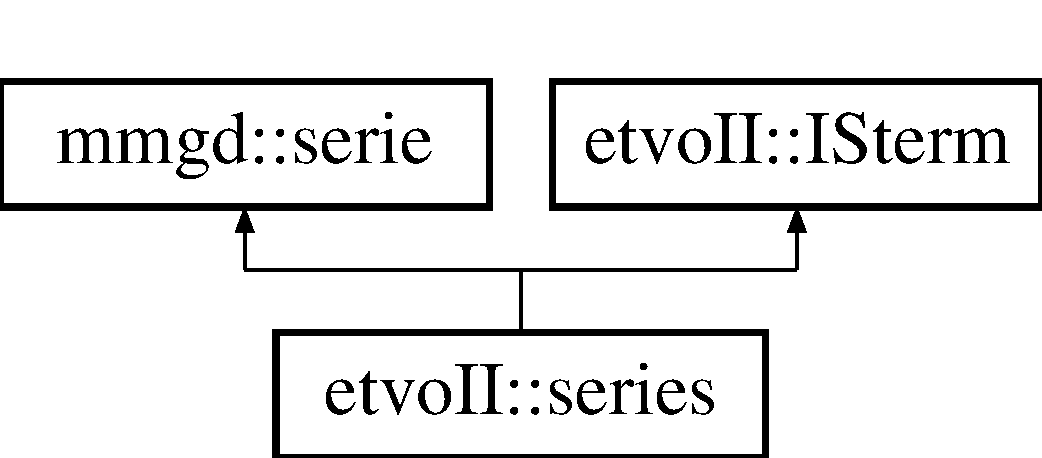
\includegraphics[height=2.000000cm]{classetvo_i_i_1_1series}
\end{center}
\end{figure}
\subsection*{Public Member Functions}
\begin{DoxyCompactItemize}
\item 
\mbox{\Hypertarget{classetvo_i_i_1_1series_ad55faeed0e6e60f6c40e4a9458795230}\label{classetvo_i_i_1_1series_ad55faeed0e6e60f6c40e4a9458795230}} 
bool {\bfseries is\+Poly} () const
\item 
\mbox{\Hypertarget{classetvo_i_i_1_1series_af1334a4b82caff1f0458b468c2d966a1}\label{classetvo_i_i_1_1series_af1334a4b82caff1f0458b468c2d966a1}} 
bool {\bfseries is\+Degenerate} () const
\item 
\mbox{\Hypertarget{classetvo_i_i_1_1series_af3c56a956329c27d606323537fe9122d}\label{classetvo_i_i_1_1series_af3c56a956329c27d606323537fe9122d}} 
{\bfseries series} (const \mbox{\hyperlink{classetvo_i_i_1_1poly}{poly}} \&p, const \mbox{\hyperlink{classetvo_i_i_1_1poly}{poly}} \&q, const \mbox{\hyperlink{classetvo_i_i_1_1gd}{gd}} \&r)
\item 
\mbox{\Hypertarget{classetvo_i_i_1_1series_ab693b0db1b3a141e4d5633e85e3ed91f}\label{classetvo_i_i_1_1series_ab693b0db1b3a141e4d5633e85e3ed91f}} 
{\bfseries series} (const \mbox{\hyperlink{classmmgd_1_1serie}{mmgd\+::serie}} \&s)
\item 
\mbox{\Hypertarget{classetvo_i_i_1_1series_a75571b7e6f2693c773412a61859eea05}\label{classetvo_i_i_1_1series_a75571b7e6f2693c773412a61859eea05}} 
{\bfseries series} (const \mbox{\hyperlink{classetvo_i_i_1_1gd}{gd}} \&)
\item 
\mbox{\Hypertarget{classetvo_i_i_1_1series_a27a88526dfdc0e5147ba43af78a2faf2}\label{classetvo_i_i_1_1series_a27a88526dfdc0e5147ba43af78a2faf2}} 
{\bfseries series} (const \mbox{\hyperlink{classetvo_i_i_1_1poly}{poly}} \&)
\item 
\mbox{\Hypertarget{classetvo_i_i_1_1series_aa7f6009dfba508eed2b8a61ff394a011}\label{classetvo_i_i_1_1series_aa7f6009dfba508eed2b8a61ff394a011}} 
{\bfseries series} (const \mbox{\hyperlink{classetvo_i_i_1_1series}{series}} \&)
\item 
\mbox{\Hypertarget{classetvo_i_i_1_1series_ac029c2e83d3990a27e75910ac2d9b9cd}\label{classetvo_i_i_1_1series_ac029c2e83d3990a27e75910ac2d9b9cd}} 
bool {\bfseries operator==} (const \mbox{\hyperlink{classetvo_i_i_1_1series}{series}} \&s) const
\item 
\mbox{\Hypertarget{classetvo_i_i_1_1series_a49f8eaf62350933b376a6fd2b51cc664}\label{classetvo_i_i_1_1series_a49f8eaf62350933b376a6fd2b51cc664}} 
bool {\bfseries operator$<$=} (const \mbox{\hyperlink{classetvo_i_i_1_1series}{series}} \&s) const
\item 
\mbox{\Hypertarget{classetvo_i_i_1_1series_ac36cba3f27c8a747b5c26b3df9b32add}\label{classetvo_i_i_1_1series_ac36cba3f27c8a747b5c26b3df9b32add}} 
bool {\bfseries operator$>$=} (const \mbox{\hyperlink{classetvo_i_i_1_1series}{series}} \&s) const
\item 
\mbox{\Hypertarget{classetvo_i_i_1_1series_ab505a24198a451b1ddb9c5c3b780d3a3}\label{classetvo_i_i_1_1series_ab505a24198a451b1ddb9c5c3b780d3a3}} 
\mbox{\hyperlink{classetvo_i_i_1_1series}{series}} {\bfseries operator+} (const \mbox{\hyperlink{classetvo_i_i_1_1series}{series}} \&s) const
\item 
\mbox{\Hypertarget{classetvo_i_i_1_1series_aa7f80e5acb3ae904ba967720ffba4c1e}\label{classetvo_i_i_1_1series_aa7f80e5acb3ae904ba967720ffba4c1e}} 
\mbox{\hyperlink{classetvo_i_i_1_1series}{series}} {\bfseries operator$\ast$} (const \mbox{\hyperlink{classetvo_i_i_1_1series}{series}} \&s) const
\item 
\mbox{\Hypertarget{classetvo_i_i_1_1series_ac4e2b6746681dd96b6f3d0db539507c8}\label{classetvo_i_i_1_1series_ac4e2b6746681dd96b6f3d0db539507c8}} 
\mbox{\hyperlink{classetvo_i_i_1_1series}{series}} {\bfseries inf} (const \mbox{\hyperlink{classetvo_i_i_1_1series}{series}} \&s) const
\item 
\mbox{\Hypertarget{classetvo_i_i_1_1series_a43f60fd9d21d86421e4124560da9572d}\label{classetvo_i_i_1_1series_a43f60fd9d21d86421e4124560da9572d}} 
\mbox{\hyperlink{classetvo_i_i_1_1series}{series}} {\bfseries star} () const
\item 
\mbox{\Hypertarget{classetvo_i_i_1_1series_a87f2e8374edd1ae4e1abe76d08423254}\label{classetvo_i_i_1_1series_a87f2e8374edd1ae4e1abe76d08423254}} 
\mbox{\hyperlink{classetvo_i_i_1_1series}{series}} {\bfseries lfrac} (const \mbox{\hyperlink{classetvo_i_i_1_1series}{series}} \&s) const
\item 
\mbox{\Hypertarget{classetvo_i_i_1_1series_a5cab5e64345d4173ebc58ba7ee01d297}\label{classetvo_i_i_1_1series_a5cab5e64345d4173ebc58ba7ee01d297}} 
\mbox{\hyperlink{classetvo_i_i_1_1series}{series}} {\bfseries rfrac} (const \mbox{\hyperlink{classetvo_i_i_1_1series}{series}} \&s) const
\item 
\mbox{\Hypertarget{classetvo_i_i_1_1series_aeb25bf6592e6c77b4ba3eb21c729f067}\label{classetvo_i_i_1_1series_aeb25bf6592e6c77b4ba3eb21c729f067}} 
\mbox{\hyperlink{classetvo_i_i_1_1series}{series}} {\bfseries frac} (const \mbox{\hyperlink{classetvo_i_i_1_1series}{series}} \&s) const
\item 
\mbox{\Hypertarget{classetvo_i_i_1_1series_af31254e3923593918c2f3791a29e9cd3}\label{classetvo_i_i_1_1series_af31254e3923593918c2f3791a29e9cd3}} 
\mbox{\hyperlink{classetvo_i_i_1_1series}{series}} {\bfseries frac} (const \mbox{\hyperlink{classetvo_i_i_1_1gd}{gd}} \&m) const
\item 
\mbox{\Hypertarget{classetvo_i_i_1_1series_a5124cc9bbc7745be2970479c0a588052}\label{classetvo_i_i_1_1series_a5124cc9bbc7745be2970479c0a588052}} 
\mbox{\hyperlink{classetvo_i_i_1_1series}{series}} {\bfseries frac} (const \mbox{\hyperlink{classetvo_i_i_1_1poly}{poly}} \&p) const
\item 
\mbox{\Hypertarget{classetvo_i_i_1_1series_a448c9581ed8ca63c795688aa1934c732}\label{classetvo_i_i_1_1series_a448c9581ed8ca63c795688aa1934c732}} 
\mbox{\hyperlink{classetvo_i_i_1_1series}{series}} {\bfseries prcaus} () const
\item 
\mbox{\Hypertarget{classetvo_i_i_1_1series_ad2101fcedbcb3e986ec5602910cb7dee}\label{classetvo_i_i_1_1series_ad2101fcedbcb3e986ec5602910cb7dee}} 
std\+::string {\bfseries To\+String} () const
\end{DoxyCompactItemize}
\subsection*{Static Public Member Functions}
\begin{DoxyCompactItemize}
\item 
\mbox{\Hypertarget{classetvo_i_i_1_1series_a4b61c527cbbb5c9365b1912f2d7f700d}\label{classetvo_i_i_1_1series_a4b61c527cbbb5c9365b1912f2d7f700d}} 
static \mbox{\hyperlink{classetvo_i_i_1_1series}{series}} {\bfseries Epsilon} ()
\item 
\mbox{\Hypertarget{classetvo_i_i_1_1series_a7ef500cc122204d82fe762e5aa260939}\label{classetvo_i_i_1_1series_a7ef500cc122204d82fe762e5aa260939}} 
static \mbox{\hyperlink{classetvo_i_i_1_1series}{series}} {\bfseries E} ()
\item 
\mbox{\Hypertarget{classetvo_i_i_1_1series_a8217c82caf53fb5cc403240b1d8b0668}\label{classetvo_i_i_1_1series_a8217c82caf53fb5cc403240b1d8b0668}} 
static \mbox{\hyperlink{classetvo_i_i_1_1series}{series}} {\bfseries Top} ()
\end{DoxyCompactItemize}
\subsection*{Additional Inherited Members}


The documentation for this class was generated from the following files\+:\begin{DoxyCompactItemize}
\item 
etvo/wrapper\+M\+M\+G\+D/series\+Wrapper.\+h\item 
etvo/wrapper\+M\+M\+G\+D/series\+Wrapper.\+cpp\end{DoxyCompactItemize}

\hypertarget{classetvo_i_i_1_1series_ed}{}\section{etvo\+II\+:\+:series\+Ed Class Reference}
\label{classetvo_i_i_1_1series_ed}\index{etvo\+I\+I\+::series\+Ed@{etvo\+I\+I\+::series\+Ed}}
Inheritance diagram for etvo\+II\+:\+:series\+Ed\+:\begin{figure}[H]
\begin{center}
\leavevmode
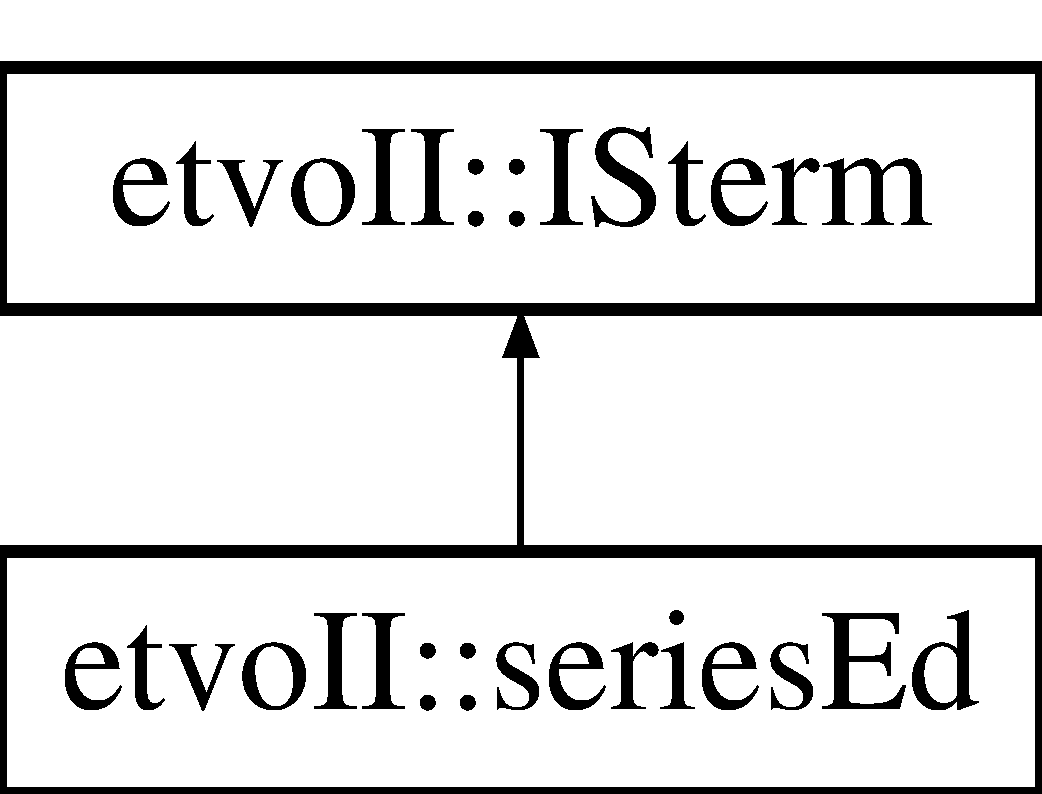
\includegraphics[height=2.000000cm]{classetvo_i_i_1_1series_ed}
\end{center}
\end{figure}
\subsection*{Public Member Functions}
\begin{DoxyCompactItemize}
\item 
\mbox{\Hypertarget{classetvo_i_i_1_1series_ed_a86e516a6ad92778dc3fd9b6d8b09a726}\label{classetvo_i_i_1_1series_ed_a86e516a6ad92778dc3fd9b6d8b09a726}} 
\mbox{\hyperlink{classetvo_i_i_1_1series_ed_a86e516a6ad92778dc3fd9b6d8b09a726}{series\+Ed}} ()
\begin{DoxyCompactList}\small\item\em epsilon \mbox{\hyperlink{classetvo_i_i_1_1series_ed}{series\+Ed}} \end{DoxyCompactList}\item 
\mbox{\Hypertarget{classetvo_i_i_1_1series_ed_a6d05a75db474ff6ba6a2f790a4a93ff0}\label{classetvo_i_i_1_1series_ed_a6d05a75db474ff6ba6a2f790a4a93ff0}} 
\mbox{\hyperlink{classetvo_i_i_1_1series_ed_a6d05a75db474ff6ba6a2f790a4a93ff0}{series\+Ed}} (bool Top\+NotE)
\begin{DoxyCompactList}\small\item\em Top (true) OR E(false) \mbox{\hyperlink{classetvo_i_i_1_1series_ed}{series\+Ed}}. \end{DoxyCompactList}\item 
\mbox{\Hypertarget{classetvo_i_i_1_1series_ed_a0945f34c4e3a7ed30a95e36e64b3f2b7}\label{classetvo_i_i_1_1series_ed_a0945f34c4e3a7ed30a95e36e64b3f2b7}} 
\mbox{\hyperlink{classetvo_i_i_1_1series_ed_a0945f34c4e3a7ed30a95e36e64b3f2b7}{series\+Ed}} (const \mbox{\hyperlink{classetvo_i_i_1_1poly_ed}{poly\+Ed}} \&p, const \mbox{\hyperlink{classetvo_i_i_1_1poly_ed}{poly\+Ed}} \&q, long gR, long d, bool right=1)
\begin{DoxyCompactList}\small\item\em \mbox{\hyperlink{classetvo_i_i_1_1series_ed}{series\+Ed}} from periodic p,q,r (right/left) form \end{DoxyCompactList}\item 
\mbox{\Hypertarget{classetvo_i_i_1_1series_ed_a2e527305328d8fc00f61a9d9f11f4105}\label{classetvo_i_i_1_1series_ed_a2e527305328d8fc00f61a9d9f11f4105}} 
{\bfseries series\+Ed} (const \mbox{\hyperlink{classetvo_i_i_1_1poly_ed}{poly\+Ed}} \&p, const \mbox{\hyperlink{classetvo_i_i_1_1poly_ed}{poly\+Ed}} \&q, const \mbox{\hyperlink{classetvo_i_i_1_1gd}{gd}} \&r, bool right=1)
\item 
\mbox{\Hypertarget{classetvo_i_i_1_1series_ed_a8a41844c37669d9e08288aeb533ba55a}\label{classetvo_i_i_1_1series_ed_a8a41844c37669d9e08288aeb533ba55a}} 
\mbox{\hyperlink{classetvo_i_i_1_1series_ed_a8a41844c37669d9e08288aeb533ba55a}{series\+Ed}} (const \mbox{\hyperlink{classetvo_i_i_1_1poly_ed}{poly\+Ed}} \&q)
\begin{DoxyCompactList}\small\item\em \mbox{\hyperlink{classetvo_i_i_1_1series_ed}{series\+Ed}} from \mbox{\hyperlink{classetvo_i_i_1_1poly_ed}{poly\+Ed}} \end{DoxyCompactList}\item 
\mbox{\Hypertarget{classetvo_i_i_1_1series_ed_a2edecb7de28f24b7c209ff0c51d86715}\label{classetvo_i_i_1_1series_ed_a2edecb7de28f24b7c209ff0c51d86715}} 
\mbox{\hyperlink{classetvo_i_i_1_1series_ed_a2edecb7de28f24b7c209ff0c51d86715}{series\+Ed}} (const \mbox{\hyperlink{classetvo_i_i_1_1_ed}{Ed}} \&m)
\begin{DoxyCompactList}\small\item\em \mbox{\hyperlink{classetvo_i_i_1_1series_ed}{series\+Ed}} from \mbox{\hyperlink{classetvo_i_i_1_1_ed}{Ed}} term \end{DoxyCompactList}\item 
\mbox{\Hypertarget{classetvo_i_i_1_1series_ed_a95587f4bea49ce6ae6f5e00e1fe2c9ee}\label{classetvo_i_i_1_1series_ed_a95587f4bea49ce6ae6f5e00e1fe2c9ee}} 
bool \mbox{\hyperlink{classetvo_i_i_1_1series_ed_a95587f4bea49ce6ae6f5e00e1fe2c9ee}{is\+Right\+Form}} () const
\begin{DoxyCompactList}\small\item\em check if in Right/\+Left form \end{DoxyCompactList}\item 
\mbox{\Hypertarget{classetvo_i_i_1_1series_ed_a5d216d120e9f079de760266bbae4f23c}\label{classetvo_i_i_1_1series_ed_a5d216d120e9f079de760266bbae4f23c}} 
bool {\bfseries is\+Left\+Form} () const
\item 
\mbox{\Hypertarget{classetvo_i_i_1_1series_ed_a49627a37de1fe2b2f0a8aac9ed0fc3c4}\label{classetvo_i_i_1_1series_ed_a49627a37de1fe2b2f0a8aac9ed0fc3c4}} 
bool \mbox{\hyperlink{classetvo_i_i_1_1series_ed_a49627a37de1fe2b2f0a8aac9ed0fc3c4}{is\+Polynomial}} () const
\begin{DoxyCompactList}\small\item\em check if it is only a polynomial \end{DoxyCompactList}\item 
\mbox{\Hypertarget{classetvo_i_i_1_1series_ed_a60aa7d381f6f35ff0e59d85d21b8a9b5}\label{classetvo_i_i_1_1series_ed_a60aa7d381f6f35ff0e59d85d21b8a9b5}} 
bool \mbox{\hyperlink{classetvo_i_i_1_1series_ed_a60aa7d381f6f35ff0e59d85d21b8a9b5}{is\+Proper}} () const
\begin{DoxyCompactList}\small\item\em check if it is in proper form \end{DoxyCompactList}\item 
\mbox{\Hypertarget{classetvo_i_i_1_1series_ed_a7253cad36e8efb6374dfd5e4341efbeb}\label{classetvo_i_i_1_1series_ed_a7253cad36e8efb6374dfd5e4341efbeb}} 
bool \mbox{\hyperlink{classetvo_i_i_1_1series_ed_a7253cad36e8efb6374dfd5e4341efbeb}{isE}} () const
\begin{DoxyCompactList}\small\item\em check if neutral \mbox{\hyperlink{classetvo_i_i_1_1series_ed}{series\+Ed}} \end{DoxyCompactList}\item 
\mbox{\Hypertarget{classetvo_i_i_1_1series_ed_af891a5c9bd4d37c263729726208d96f6}\label{classetvo_i_i_1_1series_ed_af891a5c9bd4d37c263729726208d96f6}} 
void \mbox{\hyperlink{classetvo_i_i_1_1series_ed_af891a5c9bd4d37c263729726208d96f6}{canon}} ()
\begin{DoxyCompactList}\small\item\em leads to canonical form (simplest proper form) \end{DoxyCompactList}\item 
\mbox{\Hypertarget{classetvo_i_i_1_1series_ed_a81ea31b035d4413c68d62f391221fccb}\label{classetvo_i_i_1_1series_ed_a81ea31b035d4413c68d62f391221fccb}} 
void \mbox{\hyperlink{classetvo_i_i_1_1series_ed_a81ea31b035d4413c68d62f391221fccb}{to\+Right}} ()
\begin{DoxyCompactList}\small\item\em to Right form \end{DoxyCompactList}\item 
\mbox{\Hypertarget{classetvo_i_i_1_1series_ed_acfa7eff4586cc0bafdf57222254c0d50}\label{classetvo_i_i_1_1series_ed_acfa7eff4586cc0bafdf57222254c0d50}} 
void \mbox{\hyperlink{classetvo_i_i_1_1series_ed_acfa7eff4586cc0bafdf57222254c0d50}{to\+Left}} ()
\begin{DoxyCompactList}\small\item\em to Left form \end{DoxyCompactList}\item 
\mbox{\Hypertarget{classetvo_i_i_1_1series_ed_af42bdaf41cf1c53fc325b837640bdba4}\label{classetvo_i_i_1_1series_ed_af42bdaf41cf1c53fc325b837640bdba4}} 
\mbox{\hyperlink{classetvo_i_i_1_1poly_ed}{poly\+Ed}} \mbox{\hyperlink{classetvo_i_i_1_1series_ed_af42bdaf41cf1c53fc325b837640bdba4}{getP}} () const
\begin{DoxyCompactList}\small\item\em getters returning p,q,r \end{DoxyCompactList}\item 
\mbox{\Hypertarget{classetvo_i_i_1_1series_ed_ad90c31e6dbebebeb4a0b90f8eaefcbb3}\label{classetvo_i_i_1_1series_ed_ad90c31e6dbebebeb4a0b90f8eaefcbb3}} 
\mbox{\hyperlink{classetvo_i_i_1_1poly_ed}{poly\+Ed}} {\bfseries getQ} () const
\item 
\mbox{\Hypertarget{classetvo_i_i_1_1series_ed_a6e314faaf87083611f2ff8280d27215d}\label{classetvo_i_i_1_1series_ed_a6e314faaf87083611f2ff8280d27215d}} 
\mbox{\hyperlink{classetvo_i_i_1_1gd}{gd}} {\bfseries getR} () const
\item 
\mbox{\Hypertarget{classetvo_i_i_1_1series_ed_a6d9e0bd2502b34c4ca3e6156dd880a33}\label{classetvo_i_i_1_1series_ed_a6d9e0bd2502b34c4ca3e6156dd880a33}} 
std\+::vector$<$ \mbox{\hyperlink{classetvo_i_i_1_1series}{series}} $>$ \mbox{\hyperlink{classetvo_i_i_1_1series_ed_a6d9e0bd2502b34c4ca3e6156dd880a33}{to\+Impulse\+Response}} () const
\begin{DoxyCompactList}\small\item\em returns the response to I,g1.\+I,g2.\+I ... \end{DoxyCompactList}\item 
\mbox{\Hypertarget{classetvo_i_i_1_1series_ed_adb6266ee8770bfbc37617f2c8f75d5e4}\label{classetvo_i_i_1_1series_ed_adb6266ee8770bfbc37617f2c8f75d5e4}} 
void {\bfseries get\+Lcm\+Gain} (unsigned int \&mu, unsigned int \&beta) const
\item 
\mbox{\Hypertarget{classetvo_i_i_1_1series_ed_ab325dce008db1e7d336a1a750389f6ec}\label{classetvo_i_i_1_1series_ed_ab325dce008db1e7d336a1a750389f6ec}} 
void {\bfseries get\+Max\+Gain} (unsigned int \&mu, unsigned int \&beta) const
\item 
\mbox{\Hypertarget{classetvo_i_i_1_1series_ed_a677f9e04ac56ce4cfae890e1d1e65b4a}\label{classetvo_i_i_1_1series_ed_a677f9e04ac56ce4cfae890e1d1e65b4a}} 
std\+::pair$<$ unsigned int, unsigned int $>$ {\bfseries get\+Max\+Gain} () const
\item 
\mbox{\Hypertarget{classetvo_i_i_1_1series_ed_a770bdaa263a47076abae16b8c080f13f}\label{classetvo_i_i_1_1series_ed_a770bdaa263a47076abae16b8c080f13f}} 
std\+::string {\bfseries to\+String} () const
\item 
\mbox{\Hypertarget{classetvo_i_i_1_1series_ed_a7afcc7b2231dad36b3f1be4ad7cd2335}\label{classetvo_i_i_1_1series_ed_a7afcc7b2231dad36b3f1be4ad7cd2335}} 
std\+::string {\bfseries to\+String\+As\+Mu\+Var} () const
\item 
\mbox{\Hypertarget{classetvo_i_i_1_1series_ed_adde0ba02140de943e44298bfeeb6b0d3}\label{classetvo_i_i_1_1series_ed_adde0ba02140de943e44298bfeeb6b0d3}} 
bool {\bfseries operator==} (const \mbox{\hyperlink{classetvo_i_i_1_1series_ed}{series\+Ed}} \&s) const
\item 
\mbox{\Hypertarget{classetvo_i_i_1_1series_ed_ae078b7e48c66c3f4569f44a87d438b37}\label{classetvo_i_i_1_1series_ed_ae078b7e48c66c3f4569f44a87d438b37}} 
bool {\bfseries operator!=} (const \mbox{\hyperlink{classetvo_i_i_1_1series_ed}{series\+Ed}} \&) const
\item 
\mbox{\Hypertarget{classetvo_i_i_1_1series_ed_a534eaaca3145aac56974378cc09e5636}\label{classetvo_i_i_1_1series_ed_a534eaaca3145aac56974378cc09e5636}} 
bool {\bfseries operator$<$=} (const \mbox{\hyperlink{classetvo_i_i_1_1series_ed}{series\+Ed}} \&) const
\item 
\mbox{\Hypertarget{classetvo_i_i_1_1series_ed_a1dc735d79007d07459069c24bee6a255}\label{classetvo_i_i_1_1series_ed_a1dc735d79007d07459069c24bee6a255}} 
bool {\bfseries operator$>$=} (const \mbox{\hyperlink{classetvo_i_i_1_1series_ed}{series\+Ed}} \&) const
\item 
\mbox{\Hypertarget{classetvo_i_i_1_1series_ed_a1f7405d5cbe6040f88eca3c6ad40ad15}\label{classetvo_i_i_1_1series_ed_a1f7405d5cbe6040f88eca3c6ad40ad15}} 
\mbox{\hyperlink{classetvo_i_i_1_1series_ed}{series\+Ed}} {\bfseries oplus} (const \mbox{\hyperlink{classetvo_i_i_1_1series_ed}{series\+Ed}} \&s) const
\item 
\mbox{\Hypertarget{classetvo_i_i_1_1series_ed_a3c01e83edc9c3e3b1f1b51e7e2806520}\label{classetvo_i_i_1_1series_ed_a3c01e83edc9c3e3b1f1b51e7e2806520}} 
\mbox{\hyperlink{classetvo_i_i_1_1series_ed}{series\+Ed}} {\bfseries oplus} (const \mbox{\hyperlink{classetvo_i_i_1_1poly_ed}{poly\+Ed}} \&p) const
\item 
\mbox{\Hypertarget{classetvo_i_i_1_1series_ed_a6fedde56e41656aecfe1a299b6829f9a}\label{classetvo_i_i_1_1series_ed_a6fedde56e41656aecfe1a299b6829f9a}} 
\mbox{\hyperlink{classetvo_i_i_1_1series_ed}{series\+Ed}} {\bfseries otimes} (const \mbox{\hyperlink{classetvo_i_i_1_1series_ed}{series\+Ed}} \&s) const
\item 
\mbox{\Hypertarget{classetvo_i_i_1_1series_ed_aac488576bdd3e69251ba861c65122482}\label{classetvo_i_i_1_1series_ed_aac488576bdd3e69251ba861c65122482}} 
\mbox{\hyperlink{classetvo_i_i_1_1series_ed}{series\+Ed}} {\bfseries otimes} (const \mbox{\hyperlink{classetvo_i_i_1_1_ed}{Ed}} \&m) const
\item 
\mbox{\Hypertarget{classetvo_i_i_1_1series_ed_ac4059690791fbe3adc4c84aa5576b006}\label{classetvo_i_i_1_1series_ed_ac4059690791fbe3adc4c84aa5576b006}} 
\mbox{\hyperlink{classetvo_i_i_1_1series_ed}{series\+Ed}} {\bfseries otimes} (const \mbox{\hyperlink{classetvo_i_i_1_1poly_ed}{poly\+Ed}} \&p) const
\item 
\mbox{\Hypertarget{classetvo_i_i_1_1series_ed_a5dba3fb5b080e0fd7853ac4f95a1a883}\label{classetvo_i_i_1_1series_ed_a5dba3fb5b080e0fd7853ac4f95a1a883}} 
\mbox{\hyperlink{classetvo_i_i_1_1series_ed}{series\+Ed}} {\bfseries operator+} (const \mbox{\hyperlink{classetvo_i_i_1_1series_ed}{series\+Ed}} \&s) const
\item 
\mbox{\Hypertarget{classetvo_i_i_1_1series_ed_a2b7d8cedece9a8001ed3598860ca2c9d}\label{classetvo_i_i_1_1series_ed_a2b7d8cedece9a8001ed3598860ca2c9d}} 
\mbox{\hyperlink{classetvo_i_i_1_1series_ed}{series\+Ed}} {\bfseries operator$\ast$} (const \mbox{\hyperlink{classetvo_i_i_1_1series_ed}{series\+Ed}} \&s) const
\item 
\mbox{\Hypertarget{classetvo_i_i_1_1series_ed_a0ce878483fe0a480973c7e0a49f59ceb}\label{classetvo_i_i_1_1series_ed_a0ce878483fe0a480973c7e0a49f59ceb}} 
\mbox{\hyperlink{classetvo_i_i_1_1series_ed}{series\+Ed}} {\bfseries operator$\ast$} (const \mbox{\hyperlink{classetvo_i_i_1_1_ed}{Ed}} \&m) const
\item 
\mbox{\Hypertarget{classetvo_i_i_1_1series_ed_a3397f04d7400a819277c6516c791b9b7}\label{classetvo_i_i_1_1series_ed_a3397f04d7400a819277c6516c791b9b7}} 
\mbox{\hyperlink{classetvo_i_i_1_1series_ed}{series\+Ed}} {\bfseries operator$\ast$} (const \mbox{\hyperlink{classetvo_i_i_1_1poly_ed}{poly\+Ed}} \&p) const
\item 
\mbox{\Hypertarget{classetvo_i_i_1_1series_ed_a038dc1aa0918db07ec382c099abd1c5f}\label{classetvo_i_i_1_1series_ed_a038dc1aa0918db07ec382c099abd1c5f}} 
\mbox{\hyperlink{classetvo_i_i_1_1series_ed}{series\+Ed}} {\bfseries star} () const
\item 
\mbox{\Hypertarget{classetvo_i_i_1_1series_ed_a959f5d95e0bbd784c94c20f55167db23}\label{classetvo_i_i_1_1series_ed_a959f5d95e0bbd784c94c20f55167db23}} 
\mbox{\hyperlink{classetvo_i_i_1_1series_ed}{series\+Ed}} {\bfseries star\+Alternate} () const
\item 
\mbox{\Hypertarget{classetvo_i_i_1_1series_ed_abc34bc595f23ed7f08dc44a05ecec1c1}\label{classetvo_i_i_1_1series_ed_abc34bc595f23ed7f08dc44a05ecec1c1}} 
\mbox{\hyperlink{classetvo_i_i_1_1series_ed}{series\+Ed}} {\bfseries star\+CD} () const
\item 
\mbox{\Hypertarget{classetvo_i_i_1_1series_ed_ae12a7a46a0976800a8d6bf74212e0b51}\label{classetvo_i_i_1_1series_ed_ae12a7a46a0976800a8d6bf74212e0b51}} 
\mbox{\hyperlink{classetvo_i_i_1_1series_ed}{series\+Ed}} {\bfseries star\+Poly\+Based} () const
\item 
\mbox{\Hypertarget{classetvo_i_i_1_1series_ed_a39c5f788ed254ce15285e6e270588d21}\label{classetvo_i_i_1_1series_ed_a39c5f788ed254ce15285e6e270588d21}} 
\mbox{\hyperlink{classetvo_i_i_1_1series_ed}{series\+Ed}} {\bfseries otimes\+CD} (const \mbox{\hyperlink{classetvo_i_i_1_1series_ed}{series\+Ed}} \&s) const
\item 
\mbox{\Hypertarget{classetvo_i_i_1_1series_ed_a1ad8fcfbfa8eb31db6fb63021851402c}\label{classetvo_i_i_1_1series_ed_a1ad8fcfbfa8eb31db6fb63021851402c}} 
\mbox{\hyperlink{classetvo_i_i_1_1series_ed}{series\+Ed}} {\bfseries oplus\+CD} (const \mbox{\hyperlink{classetvo_i_i_1_1series_ed}{series\+Ed}} \&s) const
\item 
\mbox{\Hypertarget{classetvo_i_i_1_1series_ed_a3495839c1cdaa59a9323bb40224afc50}\label{classetvo_i_i_1_1series_ed_a3495839c1cdaa59a9323bb40224afc50}} 
\mbox{\hyperlink{classetvo_i_i_1_1series_ed}{series\+Ed}} {\bfseries inf\+CD} (const \mbox{\hyperlink{classetvo_i_i_1_1series_ed}{series\+Ed}} \&s) const
\item 
\mbox{\Hypertarget{classetvo_i_i_1_1series_ed_abc9359be4ebddff269847c4886457064}\label{classetvo_i_i_1_1series_ed_abc9359be4ebddff269847c4886457064}} 
\mbox{\hyperlink{classetvo_i_i_1_1series_ed}{series\+Ed}} {\bfseries inf} (const \mbox{\hyperlink{classetvo_i_i_1_1series_ed}{series\+Ed}} \&s) const
\item 
\mbox{\Hypertarget{classetvo_i_i_1_1series_ed_a1ddbc2e2f2010b993d73a99224e5b1cd}\label{classetvo_i_i_1_1series_ed_a1ddbc2e2f2010b993d73a99224e5b1cd}} 
\mbox{\hyperlink{classetvo_i_i_1_1series_ed}{series\+Ed}} {\bfseries lfrac\+CD} (const \mbox{\hyperlink{classetvo_i_i_1_1series_ed}{series\+Ed}} \&s) const
\item 
\mbox{\Hypertarget{classetvo_i_i_1_1series_ed_a0a315ebe817d6b52631698f5bfd86615}\label{classetvo_i_i_1_1series_ed_a0a315ebe817d6b52631698f5bfd86615}} 
\mbox{\hyperlink{classetvo_i_i_1_1series_ed}{series\+Ed}} {\bfseries rfrac\+CD} (const \mbox{\hyperlink{classetvo_i_i_1_1series_ed}{series\+Ed}} \&s) const
\item 
\mbox{\Hypertarget{classetvo_i_i_1_1series_ed_af57c5d28e6ea68d708bc90b09d4c0959}\label{classetvo_i_i_1_1series_ed_af57c5d28e6ea68d708bc90b09d4c0959}} 
\mbox{\hyperlink{classetvo_i_i_1_1series_ed}{series\+Ed}} {\bfseries lfrac} (const \mbox{\hyperlink{classetvo_i_i_1_1series_ed}{series\+Ed}} \&s) const
\item 
\mbox{\Hypertarget{classetvo_i_i_1_1series_ed_a3a777586e69fb9eefd19ab2dd3eb6285}\label{classetvo_i_i_1_1series_ed_a3a777586e69fb9eefd19ab2dd3eb6285}} 
\mbox{\hyperlink{classetvo_i_i_1_1series_ed}{series\+Ed}} {\bfseries rfrac} (const \mbox{\hyperlink{classetvo_i_i_1_1series_ed}{series\+Ed}} \&s) const
\item 
\mbox{\Hypertarget{classetvo_i_i_1_1series_ed_a077ff3693051d2e42845615c4145231d}\label{classetvo_i_i_1_1series_ed_a077ff3693051d2e42845615c4145231d}} 
\mbox{\hyperlink{classetvo_i_i_1_1poly_ed}{poly\+Ed}} {\bfseries get\+Poly\+Up\+To} (int deltaT) const
\item 
\mbox{\Hypertarget{classetvo_i_i_1_1series_ed_a61b96fb16578e9c6b3fac992f73ba360}\label{classetvo_i_i_1_1series_ed_a61b96fb16578e9c6b3fac992f73ba360}} 
\mbox{\hyperlink{classetvo_i_i_1_1series}{series}} \mbox{\hyperlink{classetvo_i_i_1_1series_ed_a61b96fb16578e9c6b3fac992f73ba360}{to\+Series}} () const
\begin{DoxyCompactList}\small\item\em projection series\+Ed-\/$>$series (zero slice) \end{DoxyCompactList}\item 
\mbox{\Hypertarget{classetvo_i_i_1_1series_ed_ac0bc0026bddf7646f07f81ed7aa68dce}\label{classetvo_i_i_1_1series_ed_ac0bc0026bddf7646f07f81ed7aa68dce}} 
\mbox{\hyperlink{classetvo_i_i_1_1matrix}{etvo\+I\+I\+::matrix}}$<$ \mbox{\hyperlink{classetvo_i_i_1_1series}{series}} $>$ {\bfseries get\+Core} (unsigned ratio=1) const
\item 
\mbox{\Hypertarget{classetvo_i_i_1_1series_ed_a73138cafb1fe66d4e62fe4a33a81ac96}\label{classetvo_i_i_1_1series_ed_a73138cafb1fe66d4e62fe4a33a81ac96}} 
\mbox{\hyperlink{classetvo_i_i_1_1matrix}{etvo\+I\+I\+::matrix}}$<$ \mbox{\hyperlink{classetvo_i_i_1_1series}{series}} $>$ {\bfseries get\+Core\+Max} (unsigned ratio=1) const
\end{DoxyCompactItemize}
\subsection*{Static Public Member Functions}
\begin{DoxyCompactItemize}
\item 
\mbox{\Hypertarget{classetvo_i_i_1_1series_ed_a74175f2f194c76eaf1d7787d7f53be84}\label{classetvo_i_i_1_1series_ed_a74175f2f194c76eaf1d7787d7f53be84}} 
static \mbox{\hyperlink{classetvo_i_i_1_1series_ed}{series\+Ed}} \mbox{\hyperlink{classetvo_i_i_1_1series_ed_a74175f2f194c76eaf1d7787d7f53be84}{Epsilon}} ()
\begin{DoxyCompactList}\small\item\em eps,E,Top \end{DoxyCompactList}\item 
\mbox{\Hypertarget{classetvo_i_i_1_1series_ed_a6e082bdd4a46c1295f8f8617cbe6c188}\label{classetvo_i_i_1_1series_ed_a6e082bdd4a46c1295f8f8617cbe6c188}} 
static \mbox{\hyperlink{classetvo_i_i_1_1series_ed}{series\+Ed}} {\bfseries Top} ()
\item 
\mbox{\Hypertarget{classetvo_i_i_1_1series_ed_a5275f223d13fa265dccf44fe7f5d6e31}\label{classetvo_i_i_1_1series_ed_a5275f223d13fa265dccf44fe7f5d6e31}} 
static \mbox{\hyperlink{classetvo_i_i_1_1series_ed}{series\+Ed}} {\bfseries E} ()
\item 
\mbox{\Hypertarget{classetvo_i_i_1_1series_ed_a40a45e15c5059beebf89aaf0718e3dde}\label{classetvo_i_i_1_1series_ed_a40a45e15c5059beebf89aaf0718e3dde}} 
static \mbox{\hyperlink{classetvo_i_i_1_1series_ed}{series\+Ed}} {\bfseries oplus} (const \mbox{\hyperlink{classetvo_i_i_1_1poly_ed}{poly\+Ed}} \&p, const \mbox{\hyperlink{classetvo_i_i_1_1series_ed}{series\+Ed}} \&s)
\item 
\mbox{\Hypertarget{classetvo_i_i_1_1series_ed_ac42a563c3bdea96b13440d0addd97cd6}\label{classetvo_i_i_1_1series_ed_ac42a563c3bdea96b13440d0addd97cd6}} 
static \mbox{\hyperlink{classetvo_i_i_1_1series_ed}{series\+Ed}} {\bfseries otimes} (const \mbox{\hyperlink{classetvo_i_i_1_1_ed}{Ed}} \&m, const \mbox{\hyperlink{classetvo_i_i_1_1series_ed}{series\+Ed}} \&s)
\item 
\mbox{\Hypertarget{classetvo_i_i_1_1series_ed_a2e1b7e671b1baba215d5399ebc137695}\label{classetvo_i_i_1_1series_ed_a2e1b7e671b1baba215d5399ebc137695}} 
static \mbox{\hyperlink{classetvo_i_i_1_1series_ed}{series\+Ed}} {\bfseries otimes} (const \mbox{\hyperlink{classetvo_i_i_1_1poly_ed}{poly\+Ed}} \&m, const \mbox{\hyperlink{classetvo_i_i_1_1series_ed}{series\+Ed}} \&s)
\item 
\mbox{\Hypertarget{classetvo_i_i_1_1series_ed_a649ece302bf7a45481c450c2d7b1b3f1}\label{classetvo_i_i_1_1series_ed_a649ece302bf7a45481c450c2d7b1b3f1}} 
static \mbox{\hyperlink{classetvo_i_i_1_1poly_ed}{poly\+Ed}} {\bfseries get\+Poly\+Up\+To} (int deltaT, const \mbox{\hyperlink{classetvo_i_i_1_1poly_ed}{poly\+Ed}} \&p, const \mbox{\hyperlink{classetvo_i_i_1_1poly_ed}{poly\+Ed}} \&q, const \mbox{\hyperlink{classetvo_i_i_1_1gd}{gd}} \&r, bool droite=true)
\item 
\mbox{\Hypertarget{classetvo_i_i_1_1series_ed_a50c626579b815738e979fd9a22803b53}\label{classetvo_i_i_1_1series_ed_a50c626579b815738e979fd9a22803b53}} 
static \mbox{\hyperlink{classetvo_i_i_1_1series_ed}{series\+Ed}} {\bfseries to\+Causal} (const \mbox{\hyperlink{classetvo_i_i_1_1series_ed}{series\+Ed}} \&s)
\item 
\mbox{\Hypertarget{classetvo_i_i_1_1series_ed_acbeea1cf1adea319ccd09b306c0e32de}\label{classetvo_i_i_1_1series_ed_acbeea1cf1adea319ccd09b306c0e32de}} 
static \mbox{\hyperlink{classetvo_i_i_1_1series_ed}{series\+Ed}} \mbox{\hyperlink{classetvo_i_i_1_1series_ed_acbeea1cf1adea319ccd09b306c0e32de}{to\+Series\+Ed}} (const \mbox{\hyperlink{classetvo_i_i_1_1series}{series}} \&s)
\begin{DoxyCompactList}\small\item\em injection series(mmgd)-\/$>$\mbox{\hyperlink{classetvo_i_i_1_1series_ed}{series\+Ed}} \end{DoxyCompactList}\item 
\mbox{\Hypertarget{classetvo_i_i_1_1series_ed_af5ecb82703d6d70f9934f1a87a71ecc0}\label{classetvo_i_i_1_1series_ed_af5ecb82703d6d70f9934f1a87a71ecc0}} 
static \mbox{\hyperlink{classetvo_i_i_1_1series_ed}{series\+Ed}} \mbox{\hyperlink{classetvo_i_i_1_1series_ed_af5ecb82703d6d70f9934f1a87a71ecc0}{core\+To\+Series\+Ed}} (const \mbox{\hyperlink{classetvo_i_i_1_1matrix}{matrix}}$<$ \mbox{\hyperlink{classetvo_i_i_1_1series}{series}} $>$ \&C)
\begin{DoxyCompactList}\small\item\em conversion C\+O\+RE decomposition -\/$>$ \mbox{\hyperlink{classetvo_i_i_1_1series_ed}{series\+Ed}} \end{DoxyCompactList}\item 
\mbox{\Hypertarget{classetvo_i_i_1_1series_ed_a3aa0bf3e47c852e5a4095de23fc3dd19}\label{classetvo_i_i_1_1series_ed_a3aa0bf3e47c852e5a4095de23fc3dd19}} 
static \mbox{\hyperlink{classetvo_i_i_1_1matrix}{etvo\+I\+I\+::matrix}}$<$ \mbox{\hyperlink{classetvo_i_i_1_1series}{series}} $>$ {\bfseries get\+MatN} (unsigned size)
\end{DoxyCompactItemize}
\subsection*{Additional Inherited Members}


The documentation for this class was generated from the following files\+:\begin{DoxyCompactItemize}
\item 
etvo/series\+Ed/series\+Ed.\+h\item 
etvo/series\+Ed/series\+Ed.\+cpp\end{DoxyCompactItemize}

\hypertarget{classetvo_i_i_1_1_t__op}{}\section{etvo\+II\+:\+:T\+\_\+op Class Reference}
\label{classetvo_i_i_1_1_t__op}\index{etvo\+I\+I\+::\+T\+\_\+op@{etvo\+I\+I\+::\+T\+\_\+op}}
\subsection*{Public Member Functions}
\begin{DoxyCompactItemize}
\item 
\mbox{\Hypertarget{classetvo_i_i_1_1_t__op_a8381627b92222fe5fa7c3ad4e07bc7e8}\label{classetvo_i_i_1_1_t__op_a8381627b92222fe5fa7c3ad4e07bc7e8}} 
\mbox{\hyperlink{classetvo_i_i_1_1_t__op_a8381627b92222fe5fa7c3ad4e07bc7e8}{T\+\_\+op}} ()
\begin{DoxyCompactList}\small\item\em E op. \end{DoxyCompactList}\item 
\mbox{\Hypertarget{classetvo_i_i_1_1_t__op_afa7715276693e1d5105335a660f72291}\label{classetvo_i_i_1_1_t__op_afa7715276693e1d5105335a660f72291}} 
{\bfseries T\+\_\+op} (const \mbox{\hyperlink{classetvo_i_i_1_1d_dd}{d\+Dd}} \&term)
\item 
\mbox{\Hypertarget{classetvo_i_i_1_1_t__op_a9acc9d283812511eb94af19e114e2c40}\label{classetvo_i_i_1_1_t__op_a9acc9d283812511eb94af19e114e2c40}} 
void {\bfseries add} (const \mbox{\hyperlink{classetvo_i_i_1_1d_dd}{d\+Dd}} \&term)
\item 
\mbox{\Hypertarget{classetvo_i_i_1_1_t__op_aaf851da3708d18f38e034c0453c1153f}\label{classetvo_i_i_1_1_t__op_aaf851da3708d18f38e034c0453c1153f}} 
void {\bfseries add} (const \mbox{\hyperlink{classetvo_i_i_1_1_t__op}{T\+\_\+op}} \&op)
\item 
\mbox{\Hypertarget{classetvo_i_i_1_1_t__op_a33b2270ebe289302866b4da5a08ad751}\label{classetvo_i_i_1_1_t__op_a33b2270ebe289302866b4da5a08ad751}} 
std\+::pair$<$ unsigned, unsigned $>$ {\bfseries get\+Periodicity} () const
\item 
\mbox{\Hypertarget{classetvo_i_i_1_1_t__op_ab6692ede8f4210c4f136be21fc0b23aa}\label{classetvo_i_i_1_1_t__op_ab6692ede8f4210c4f136be21fc0b23aa}} 
std\+::vector$<$ \mbox{\hyperlink{classetvo_i_i_1_1d_dd}{d\+Dd}} $>$ {\bfseries get\+Terms} () const
\item 
\mbox{\Hypertarget{classetvo_i_i_1_1_t__op_a4993c538d84002b8f96cc69c7004e0bc}\label{classetvo_i_i_1_1_t__op_a4993c538d84002b8f96cc69c7004e0bc}} 
unsigned {\bfseries get\+MB} () const
\item 
\mbox{\Hypertarget{classetvo_i_i_1_1_t__op_acfacc00c2fe584ce4c346efba88737cd}\label{classetvo_i_i_1_1_t__op_acfacc00c2fe584ce4c346efba88737cd}} 
\mbox{\hyperlink{classetvo_i_i_1_1_t__op}{T\+\_\+op}} {\bfseries extend\+By} (unsigned mul) const
\item 
\mbox{\Hypertarget{classetvo_i_i_1_1_t__op_a2514dfcfe122517550d5dbf502e732c4}\label{classetvo_i_i_1_1_t__op_a2514dfcfe122517550d5dbf502e732c4}} 
void {\bfseries reduce} ()
\item 
\mbox{\Hypertarget{classetvo_i_i_1_1_t__op_a4c6b75eda1d20c304d90edec477f02fe}\label{classetvo_i_i_1_1_t__op_a4c6b75eda1d20c304d90edec477f02fe}} 
std\+::string {\bfseries to\+String} () const
\item 
\mbox{\Hypertarget{classetvo_i_i_1_1_t__op_a54d6146732a16f43726b125bb7d91fa7}\label{classetvo_i_i_1_1_t__op_a54d6146732a16f43726b125bb7d91fa7}} 
std\+::string {\bfseries to\+String\+As\+Delta\+Var} () const
\item 
\mbox{\Hypertarget{classetvo_i_i_1_1_t__op_a876c41cfac923c76127affdfdc7c0f4c}\label{classetvo_i_i_1_1_t__op_a876c41cfac923c76127affdfdc7c0f4c}} 
int {\bfseries Rw} (int ki) const
\item 
\mbox{\Hypertarget{classetvo_i_i_1_1_t__op_a59dc7d0196c8d31b8d3a4de3d4587f61}\label{classetvo_i_i_1_1_t__op_a59dc7d0196c8d31b8d3a4de3d4587f61}} 
\mbox{\hyperlink{classetvo_i_i_1_1_fmaxp}{Fmaxp}} {\bfseries get\+Rw} () const
\item 
\mbox{\Hypertarget{classetvo_i_i_1_1_t__op_aa04aa56e4980fcf804a76afbdd510570}\label{classetvo_i_i_1_1_t__op_aa04aa56e4980fcf804a76afbdd510570}} 
void {\bfseries set\+From\+Rw} (const \mbox{\hyperlink{classetvo_i_i_1_1_fmaxp}{Fmaxp}} \&)
\item 
\mbox{\Hypertarget{classetvo_i_i_1_1_t__op_a9df66a448c2cc32d94d92900af2ba94b}\label{classetvo_i_i_1_1_t__op_a9df66a448c2cc32d94d92900af2ba94b}} 
\mbox{\hyperlink{classetvo_i_i_1_1_t__op}{T\+\_\+op}} {\bfseries operator+} (const \mbox{\hyperlink{classetvo_i_i_1_1_t__op}{T\+\_\+op}} \&f) const
\item 
\mbox{\Hypertarget{classetvo_i_i_1_1_t__op_a2b52baefea1e120180ca54633cc60fd3}\label{classetvo_i_i_1_1_t__op_a2b52baefea1e120180ca54633cc60fd3}} 
\mbox{\hyperlink{classetvo_i_i_1_1_t__op}{T\+\_\+op}} {\bfseries oplus} (const \mbox{\hyperlink{classetvo_i_i_1_1_t__op}{T\+\_\+op}} \&f) const
\item 
\mbox{\Hypertarget{classetvo_i_i_1_1_t__op_af3b1b79180f037d2e6c18fdbf28a02f9}\label{classetvo_i_i_1_1_t__op_af3b1b79180f037d2e6c18fdbf28a02f9}} 
\mbox{\hyperlink{classetvo_i_i_1_1_t__op}{T\+\_\+op}} {\bfseries inf} (const \mbox{\hyperlink{classetvo_i_i_1_1_t__op}{T\+\_\+op}} \&f) const
\item 
\mbox{\Hypertarget{classetvo_i_i_1_1_t__op_a4cccae9d697f121fc4c90c4c2ad289d4}\label{classetvo_i_i_1_1_t__op_a4cccae9d697f121fc4c90c4c2ad289d4}} 
\mbox{\hyperlink{classetvo_i_i_1_1_t__op}{T\+\_\+op}} {\bfseries operator$\ast$} (const \mbox{\hyperlink{classetvo_i_i_1_1_t__op}{T\+\_\+op}} \&f) const
\item 
\mbox{\Hypertarget{classetvo_i_i_1_1_t__op_aa9de2029e624c8df97d72bacbee4eec2}\label{classetvo_i_i_1_1_t__op_aa9de2029e624c8df97d72bacbee4eec2}} 
\mbox{\hyperlink{classetvo_i_i_1_1_t__op}{T\+\_\+op}} {\bfseries otimes} (const \mbox{\hyperlink{classetvo_i_i_1_1_t__op}{T\+\_\+op}} \&f) const
\item 
\mbox{\Hypertarget{classetvo_i_i_1_1_t__op_aecef9988d7b4d0369cf0d1b8758a2bb1}\label{classetvo_i_i_1_1_t__op_aecef9988d7b4d0369cf0d1b8758a2bb1}} 
\mbox{\hyperlink{classetvo_i_i_1_1_t__op}{T\+\_\+op}} {\bfseries lfrac} (const \mbox{\hyperlink{classetvo_i_i_1_1_t__op}{T\+\_\+op}} \&f) const
\item 
\mbox{\Hypertarget{classetvo_i_i_1_1_t__op_a6947e2d92114dd3cafb0023b41ee7e0e}\label{classetvo_i_i_1_1_t__op_a6947e2d92114dd3cafb0023b41ee7e0e}} 
\mbox{\hyperlink{classetvo_i_i_1_1_t__op}{T\+\_\+op}} {\bfseries rfrac} (const \mbox{\hyperlink{classetvo_i_i_1_1_t__op}{T\+\_\+op}} \&f) const
\item 
\mbox{\Hypertarget{classetvo_i_i_1_1_t__op_a5a709ea67a9cbb7b36b02db8165e80d3}\label{classetvo_i_i_1_1_t__op_a5a709ea67a9cbb7b36b02db8165e80d3}} 
bool {\bfseries operator==} (const \mbox{\hyperlink{classetvo_i_i_1_1_t__op}{T\+\_\+op}} \&w) const
\item 
\mbox{\Hypertarget{classetvo_i_i_1_1_t__op_ae26ceb25c3765824c3730f40934fd9ce}\label{classetvo_i_i_1_1_t__op_ae26ceb25c3765824c3730f40934fd9ce}} 
bool {\bfseries operator$<$=} (const \mbox{\hyperlink{classetvo_i_i_1_1_t__op}{T\+\_\+op}} \&w) const
\item 
\mbox{\Hypertarget{classetvo_i_i_1_1_t__op_a47cf0e8c07a93db006871fead09eb77c}\label{classetvo_i_i_1_1_t__op_a47cf0e8c07a93db006871fead09eb77c}} 
bool {\bfseries operator$>$=} (const \mbox{\hyperlink{classetvo_i_i_1_1_t__op}{T\+\_\+op}} \&w) const
\item 
\mbox{\Hypertarget{classetvo_i_i_1_1_t__op_ae76b09a976629051bb98fc0fe7249fa6}\label{classetvo_i_i_1_1_t__op_ae76b09a976629051bb98fc0fe7249fa6}} 
bool {\bfseries operator$>$} (const \mbox{\hyperlink{classetvo_i_i_1_1_t__op}{T\+\_\+op}} \&w) const
\item 
\mbox{\Hypertarget{classetvo_i_i_1_1_t__op_a35e4ef6314038b7797e59cb2defce4c8}\label{classetvo_i_i_1_1_t__op_a35e4ef6314038b7797e59cb2defce4c8}} 
bool {\bfseries operator$<$} (const \mbox{\hyperlink{classetvo_i_i_1_1_t__op}{T\+\_\+op}} \&w) const
\end{DoxyCompactItemize}
\subsection*{Static Public Member Functions}
\begin{DoxyCompactItemize}
\item 
\mbox{\Hypertarget{classetvo_i_i_1_1_t__op_ae07676762447f306429a5cee4057dd2e}\label{classetvo_i_i_1_1_t__op_ae07676762447f306429a5cee4057dd2e}} 
static \mbox{\hyperlink{classetvo_i_i_1_1_t__op}{T\+\_\+op}} \mbox{\hyperlink{classetvo_i_i_1_1_t__op_ae07676762447f306429a5cee4057dd2e}{E}} ()
\begin{DoxyCompactList}\small\item\em neutral \mbox{\hyperlink{classetvo_i_i_1_1_t__op}{T\+\_\+op}} \end{DoxyCompactList}\item 
\mbox{\Hypertarget{classetvo_i_i_1_1_t__op_aebfcd131e3715e02e82dc3da9499e5b1}\label{classetvo_i_i_1_1_t__op_aebfcd131e3715e02e82dc3da9499e5b1}} 
static \mbox{\hyperlink{classetvo_i_i_1_1_t__op}{T\+\_\+op}} \mbox{\hyperlink{classetvo_i_i_1_1_t__op_aebfcd131e3715e02e82dc3da9499e5b1}{Delta}} (unsigned mb)
\begin{DoxyCompactList}\small\item\em Delta\+\_\+mb. \end{DoxyCompactList}\item 
\mbox{\Hypertarget{classetvo_i_i_1_1_t__op_ad78351eb96e65281f8bc96b09788f18a}\label{classetvo_i_i_1_1_t__op_ad78351eb96e65281f8bc96b09788f18a}} 
static \mbox{\hyperlink{classetvo_i_i_1_1_t__op}{T\+\_\+op}} \mbox{\hyperlink{classetvo_i_i_1_1_t__op_ad78351eb96e65281f8bc96b09788f18a}{delta}} (int t)
\begin{DoxyCompactList}\small\item\em delta$^\wedge$t \end{DoxyCompactList}\item 
\mbox{\Hypertarget{classetvo_i_i_1_1_t__op_aa0e83781b7a2023c99b80e6c37bda384}\label{classetvo_i_i_1_1_t__op_aa0e83781b7a2023c99b80e6c37bda384}} 
static \mbox{\hyperlink{classetvo_i_i_1_1_t__op}{T\+\_\+op}} \mbox{\hyperlink{classetvo_i_i_1_1_t__op_aa0e83781b7a2023c99b80e6c37bda384}{delta\+Var}} (const std\+::vector$<$ int $>$ \&delays)
\begin{DoxyCompactList}\small\item\em delta$^\wedge$$<$t1,t2..$>$ \end{DoxyCompactList}\end{DoxyCompactItemize}
\subsection*{Protected Attributes}
\begin{DoxyCompactItemize}
\item 
\mbox{\Hypertarget{classetvo_i_i_1_1_t__op_a1c7941be85342bad8476cf4be8fce3c5}\label{classetvo_i_i_1_1_t__op_a1c7941be85342bad8476cf4be8fce3c5}} 
\mbox{\hyperlink{classetvo_i_i_1_1_fmaxp}{Fmaxp}} {\bfseries \+\_\+fper}
\end{DoxyCompactItemize}


The documentation for this class was generated from the following files\+:\begin{DoxyCompactItemize}
\item 
etvo/etop/T\+\_\+op.\+h\item 
etvo/etop/T\+\_\+op.\+cpp\end{DoxyCompactItemize}

\section{mmgd\+:\+:taille\+\_\+incorrecte Class Reference}
\label{classmmgd_1_1taille__incorrecte}\index{mmgd\+::taille\+\_\+incorrecte@{mmgd\+::taille\+\_\+incorrecte}}
\subsection*{Public Member Functions}
\begin{DoxyCompactItemize}
\item 
\mbox{\label{classmmgd_1_1taille__incorrecte_a386ba698f1fbf5c24a7d5dae2bd82cf9}} 
{\bfseries taille\+\_\+incorrecte} (int i)
\end{DoxyCompactItemize}
\subsection*{Public Attributes}
\begin{DoxyCompactItemize}
\item 
\mbox{\label{classmmgd_1_1taille__incorrecte_a7e7428f326edd8e504a84cd90ff931eb}} 
int {\bfseries erreur}
\end{DoxyCompactItemize}


The documentation for this class was generated from the following file\+:\begin{DoxyCompactItemize}
\item 
F\+:/\+U\+A Box/\+Dev\+Soft/etvo\+I\+I\+I/etvo21/etvo/libminmaxgd/include/gd.\+h\end{DoxyCompactItemize}

\hypertarget{classtest_1_1_test}{}\section{test\+:\+:Test Class Reference}
\label{classtest_1_1_test}\index{test\+::\+Test@{test\+::\+Test}}
\subsection*{Classes}
\begin{DoxyCompactItemize}
\item 
class \mbox{\hyperlink{classtest_1_1_test_1_1_test_poly_ed}{Test\+Poly\+Ed}}
\item 
class \mbox{\hyperlink{classtest_1_1_test_1_1_test_series_ed}{Test\+Series\+Ed}}
\end{DoxyCompactItemize}
\subsection*{Static Public Member Functions}
\begin{DoxyCompactItemize}
\item 
\mbox{\Hypertarget{classtest_1_1_test_a1c025337939a36bee29e64da9edf1bcc}\label{classtest_1_1_test_a1c025337939a36bee29e64da9edf1bcc}} 
static bool {\bfseries Regular\+\_\+\+Fminp} (unsigned)
\item 
\mbox{\Hypertarget{classtest_1_1_test_aaa56ab62ca5de9bdef42de2557edd2cb}\label{classtest_1_1_test_aaa56ab62ca5de9bdef42de2557edd2cb}} 
static bool {\bfseries Regular\+\_\+\+Fmaxp} (unsigned)
\item 
\mbox{\Hypertarget{classtest_1_1_test_aaa7c69e3b00ffbe4c65e717896fa9beb}\label{classtest_1_1_test_aaa7c69e3b00ffbe4c65e717896fa9beb}} 
static void {\bfseries Test\+Regression} ()
\item 
\mbox{\Hypertarget{classtest_1_1_test_ab7f3e76eefb76dd927c98137cdba52bb}\label{classtest_1_1_test_ab7f3e76eefb76dd927c98137cdba52bb}} 
static void {\bfseries Test\+Regular} ()
\item 
\mbox{\Hypertarget{classtest_1_1_test_aabd2cd29eff0890aceabc99963d8a331}\label{classtest_1_1_test_aabd2cd29eff0890aceabc99963d8a331}} 
static void {\bfseries Test\+Pov} ()
\item 
\mbox{\Hypertarget{classtest_1_1_test_a4b160ab1f7ea4cd798e27b4ec4c50244}\label{classtest_1_1_test_a4b160ab1f7ea4cd798e27b4ec4c50244}} 
static void {\bfseries Test\+Rand\+Gen} (unsigned n\+Iter)
\item 
\mbox{\Hypertarget{classtest_1_1_test_a8bf8e3d8c74e8ba95e7ff928540fca7f}\label{classtest_1_1_test_a8bf8e3d8c74e8ba95e7ff928540fca7f}} 
static void {\bfseries Test\+Bugs} ()
\item 
\mbox{\Hypertarget{classtest_1_1_test_a731a1ba2ac4ccba93f5caa760a7d1ac9}\label{classtest_1_1_test_a731a1ba2ac4ccba93f5caa760a7d1ac9}} 
static void {\bfseries Test\+Basic\+Poly} ()
\item 
\mbox{\Hypertarget{classtest_1_1_test_ae9ef88424e87e06e51e67eabdeb8e508}\label{classtest_1_1_test_ae9ef88424e87e06e51e67eabdeb8e508}} 
static void {\bfseries Test\+Basic\+Series\+Ed} ()
\item 
\mbox{\Hypertarget{classtest_1_1_test_a31cf29564c2b74f78644f89442baabae}\label{classtest_1_1_test_a31cf29564c2b74f78644f89442baabae}} 
static void {\bfseries Test\+Canon\+Series\+Ed} (unsigned n\+Iter)
\item 
\mbox{\Hypertarget{classtest_1_1_test_a478b16331ff880bf8bff42ada9c79fb8}\label{classtest_1_1_test_a478b16331ff880bf8bff42ada9c79fb8}} 
static void {\bfseries Test\+Core\+Series\+Ed} (unsigned n\+Iter)
\item 
\mbox{\Hypertarget{classtest_1_1_test_a8b9dd01b07efe65694828b65cb863702}\label{classtest_1_1_test_a8b9dd01b07efe65694828b65cb863702}} 
static void {\bfseries Test\+All} ()
\item 
\mbox{\Hypertarget{classtest_1_1_test_a5f0c4a7d23d9b300635d8b2b047bcb5c}\label{classtest_1_1_test_a5f0c4a7d23d9b300635d8b2b047bcb5c}} 
static bool {\bfseries Regular\+\_\+poly\+Wrapper} (unsigned nb\+Iter, unsigned char T\+ST=0x0\+F)
\item 
\mbox{\Hypertarget{classtest_1_1_test_a5811fdd54af42c504d5931166da983af}\label{classtest_1_1_test_a5811fdd54af42c504d5931166da983af}} 
static bool {\bfseries Regular\+\_\+serie\+Wrapper} (unsigned nb\+Iter, unsigned char T\+ST=0x0\+F)
\item 
\mbox{\Hypertarget{classtest_1_1_test_a093d0df39f9580c662348583d1586abe}\label{classtest_1_1_test_a093d0df39f9580c662348583d1586abe}} 
static bool {\bfseries Specific\+\_\+g\+Ng} (unsigned nb\+Iter)
\item 
\mbox{\Hypertarget{classtest_1_1_test_ad740bf243567502508c2bbbd4d7f212f}\label{classtest_1_1_test_ad740bf243567502508c2bbbd4d7f212f}} 
static bool {\bfseries Specific\+\_\+d\+Dd} (unsigned nb\+Iter)
\item 
\mbox{\Hypertarget{classtest_1_1_test_a42cdd908c6aabdd0fedcf8f3c9c452f3}\label{classtest_1_1_test_a42cdd908c6aabdd0fedcf8f3c9c452f3}} 
static bool {\bfseries Specific\+\_\+poly\+Ed} (unsigned nb\+Iter)
\item 
\mbox{\Hypertarget{classtest_1_1_test_a166b428346bda678c4b39b20192ddc31}\label{classtest_1_1_test_a166b428346bda678c4b39b20192ddc31}} 
static bool {\bfseries Regular\+\_\+poly\+Ed} (unsigned, unsigned short T\+ST=0x0\+F)
\item 
\mbox{\Hypertarget{classtest_1_1_test_aac04d90279c3349fedca2cfe670c1970}\label{classtest_1_1_test_aac04d90279c3349fedca2cfe670c1970}} 
static bool {\bfseries Regular\+\_\+series\+Ed} (unsigned nb\+Iter, unsigned short T\+ST)
\item 
\mbox{\Hypertarget{classtest_1_1_test_a07ea710535261fc55b0dbacc8d34ea99}\label{classtest_1_1_test_a07ea710535261fc55b0dbacc8d34ea99}} 
static bool {\bfseries Specific\+\_\+poly\+Tg} (unsigned nb\+Iter)
\item 
\mbox{\Hypertarget{classtest_1_1_test_a7aaed77b8a4d6a959f42fc036ef75abe}\label{classtest_1_1_test_a7aaed77b8a4d6a959f42fc036ef75abe}} 
static bool {\bfseries Regular\+\_\+poly\+Tg} (unsigned, unsigned short T\+ST=0x0\+F)
\end{DoxyCompactItemize}


The documentation for this class was generated from the following files\+:\begin{DoxyCompactItemize}
\item 
etvo/test/Test.\+h\item 
etvo/test/Test.\+cpp\item 
etvo/test/\+Test\+Common/Test\+Bugs.\+cpp\item 
etvo/test/\+Test\+Common/Test\+Pov.\+cpp\item 
etvo/test/\+Test\+Common/Test\+Rand\+Gen.\+cpp\item 
etvo/test/\+Test\+E\+T\+V\+O\+P/Test\+Specificg\+Ngd\+Dd.\+cpp\item 
etvo/test/\+Test\+Fper/Test\+Fper\+Fmax\+Fmin.\+cpp\item 
etvo/test/\+Test\+M\+M\+G\+D/Test\+Wrapper\+M\+M\+G\+D.\+cpp\item 
etvo/test/Test\+Regression.\+cpp\item 
etvo/test/Test\+Regular.\+cpp\item 
etvo/test/\+Test\+Series\+Ed/Test\+Basic\+Poly.\+cpp\item 
etvo/test/\+Test\+Series\+Ed/Test\+Basic\+Series\+Ed.\+cpp\item 
etvo/test/\+Test\+Series\+Ed/Test\+Canon\+Series\+Ed.\+cpp\item 
etvo/test/\+Test\+Series\+Ed/Test\+Core\+Series\+Ed.\+cpp\item 
etvo/test/\+Test\+Series\+Ed/Test\+Series\+Ed.\+cpp\item 
etvo/test/\+Test\+Series\+Tg/Test\+Series\+Tg.\+cpp\end{DoxyCompactItemize}

\hypertarget{classtest_1_1test_exception}{}\section{test\+:\+:test\+Exception Class Reference}
\label{classtest_1_1test_exception}\index{test\+::test\+Exception@{test\+::test\+Exception}}
Inheritance diagram for test\+:\+:test\+Exception\+:\begin{figure}[H]
\begin{center}
\leavevmode
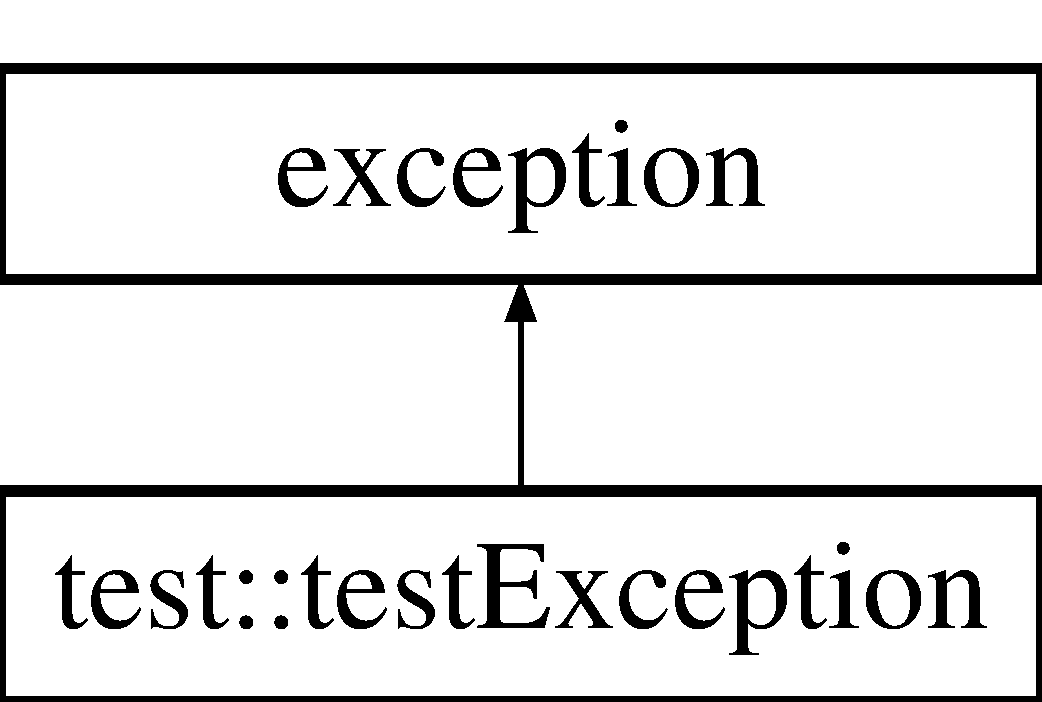
\includegraphics[height=2.000000cm]{classtest_1_1test_exception}
\end{center}
\end{figure}
\subsection*{Public Member Functions}
\begin{DoxyCompactItemize}
\item 
\mbox{\Hypertarget{classtest_1_1test_exception_aef9108e6feece2c8476c1c3d09b0f0ed}\label{classtest_1_1test_exception_aef9108e6feece2c8476c1c3d09b0f0ed}} 
{\bfseries test\+Exception} (unsigned num, const std\+::string \&msg)
\item 
\mbox{\Hypertarget{classtest_1_1test_exception_a1c64f3bd64d3d6bbb461ae2e333e6555}\label{classtest_1_1test_exception_a1c64f3bd64d3d6bbb461ae2e333e6555}} 
unsigned {\bfseries Num} () const
\item 
\mbox{\Hypertarget{classtest_1_1test_exception_ad58ece655ba80e4a9d2c20637afb3039}\label{classtest_1_1test_exception_ad58ece655ba80e4a9d2c20637afb3039}} 
std\+::string {\bfseries Message} () const
\end{DoxyCompactItemize}


The documentation for this class was generated from the following files\+:\begin{DoxyCompactItemize}
\item 
etvo/test/test\+Exception.\+h\item 
etvo/test/test\+Exception.\+cpp\end{DoxyCompactItemize}

\hypertarget{classtest_1_1_test_i_s}{}\section{test\+:\+:Test\+IS$<$ T $>$ Class Template Reference}
\label{classtest_1_1_test_i_s}\index{test\+::\+Test\+I\+S$<$ T $>$@{test\+::\+Test\+I\+S$<$ T $>$}}
\subsection*{Static Public Member Functions}
\begin{DoxyCompactItemize}
\item 
\mbox{\Hypertarget{classtest_1_1_test_i_s_aa0ee864672dd78ad0778ff450d979a4a}\label{classtest_1_1_test_i_s_aa0ee864672dd78ad0778ff450d979a4a}} 
static bool {\bfseries Test\+All} (const T \&a, const T \&b, const T \&c)
\item 
\mbox{\Hypertarget{classtest_1_1_test_i_s_adba68d4fe4f91ee465e662ec6939aa60}\label{classtest_1_1_test_i_s_adba68d4fe4f91ee465e662ec6939aa60}} 
static void {\bfseries print} (const T \&a, const T \&b)
\item 
\mbox{\Hypertarget{classtest_1_1_test_i_s_a0cff96e5b9e87c82ced013f9a45e780a}\label{classtest_1_1_test_i_s_a0cff96e5b9e87c82ced013f9a45e780a}} 
static void {\bfseries print} (const T \&a, const T \&b, const T \&c)
\item 
\mbox{\Hypertarget{classtest_1_1_test_i_s_a0a3d6f076ab302ddb247f957df47e49f}\label{classtest_1_1_test_i_s_a0a3d6f076ab302ddb247f957df47e49f}} 
static void {\bfseries Test3} (const T \&a, const T \&b)
\item 
\mbox{\Hypertarget{classtest_1_1_test_i_s_aca6ce7bc92e31a738f20f9c4b8c109ae}\label{classtest_1_1_test_i_s_aca6ce7bc92e31a738f20f9c4b8c109ae}} 
static void {\bfseries Test2} (const T \&a, const T \&b, const T \&c)
\item 
\mbox{\Hypertarget{classtest_1_1_test_i_s_a0d74db6c2f7566d7a548b18d0a59428c}\label{classtest_1_1_test_i_s_a0d74db6c2f7566d7a548b18d0a59428c}} 
static void {\bfseries Test1} (const T \&a, const T \&b)
\end{DoxyCompactItemize}


The documentation for this class was generated from the following file\+:\begin{DoxyCompactItemize}
\item 
etvo/test/\+Test\+Template/Test\+I\+S.\+h\end{DoxyCompactItemize}

\hypertarget{classtest_1_1_test_kleene}{}\section{test\+:\+:Test\+Kleene$<$ T $>$ Class Template Reference}
\label{classtest_1_1_test_kleene}\index{test\+::\+Test\+Kleene$<$ T $>$@{test\+::\+Test\+Kleene$<$ T $>$}}
\subsection*{Static Public Member Functions}
\begin{DoxyCompactItemize}
\item 
\mbox{\Hypertarget{classtest_1_1_test_kleene_aa77c20aa8b5a25d5152591aadc9e6bf6}\label{classtest_1_1_test_kleene_aa77c20aa8b5a25d5152591aadc9e6bf6}} 
static bool \mbox{\hyperlink{classtest_1_1_test_kleene_aa77c20aa8b5a25d5152591aadc9e6bf6}{Test\+All}} (const T \&a, const T \&b)
\begin{DoxyCompactList}\small\item\em a Gain 1, b Gain free \end{DoxyCompactList}\item 
\mbox{\Hypertarget{classtest_1_1_test_kleene_a0f6773f01e2e8c9c1c86db2c7daaa560}\label{classtest_1_1_test_kleene_a0f6773f01e2e8c9c1c86db2c7daaa560}} 
static void {\bfseries print} (const T \&a)
\item 
\mbox{\Hypertarget{classtest_1_1_test_kleene_aa6f233a0daee33b4fcddb249cb73cd8a}\label{classtest_1_1_test_kleene_aa6f233a0daee33b4fcddb249cb73cd8a}} 
static void {\bfseries Test1} (const T \&a)
\item 
\mbox{\Hypertarget{classtest_1_1_test_kleene_a85320079dc05edffd0df34eb5e079fa0}\label{classtest_1_1_test_kleene_a85320079dc05edffd0df34eb5e079fa0}} 
static void {\bfseries Test2} (const T \&a)
\end{DoxyCompactItemize}


The documentation for this class was generated from the following file\+:\begin{DoxyCompactItemize}
\item 
etvo/test/\+Test\+Template/Test\+Kleene.\+h\end{DoxyCompactItemize}

\hypertarget{classtest_1_1_test_1_1_test_poly_ed}{}\section{test\+:\+:Test\+:\+:Test\+Poly\+Ed Class Reference}
\label{classtest_1_1_test_1_1_test_poly_ed}\index{test\+::\+Test\+::\+Test\+Poly\+Ed@{test\+::\+Test\+::\+Test\+Poly\+Ed}}
\subsection*{Static Public Member Functions}
\begin{DoxyCompactItemize}
\item 
\mbox{\Hypertarget{classtest_1_1_test_1_1_test_poly_ed_a54a519e928514d6042cb285291b3a76f}\label{classtest_1_1_test_1_1_test_poly_ed_a54a519e928514d6042cb285291b3a76f}} 
static void {\bfseries Test\+Oplus} (unsigned n\+Iter)
\item 
\mbox{\Hypertarget{classtest_1_1_test_1_1_test_poly_ed_a8b03f6f328e379f9ee02da2cb0557917}\label{classtest_1_1_test_1_1_test_poly_ed_a8b03f6f328e379f9ee02da2cb0557917}} 
static void {\bfseries Test\+Otimes} (unsigned n\+Iter)
\item 
\mbox{\Hypertarget{classtest_1_1_test_1_1_test_poly_ed_ad4294e8e7c4bae5d2540cd85da62b708}\label{classtest_1_1_test_1_1_test_poly_ed_ad4294e8e7c4bae5d2540cd85da62b708}} 
static void {\bfseries Test\+Oplus\+PP} (unsigned n\+Iter)
\item 
\mbox{\Hypertarget{classtest_1_1_test_1_1_test_poly_ed_aa5d215f4ab4312f6d09893c3f44449a9}\label{classtest_1_1_test_1_1_test_poly_ed_aa5d215f4ab4312f6d09893c3f44449a9}} 
static void {\bfseries Test\+Comp\+Frac} (unsigned int n\+Iter)
\item 
\mbox{\Hypertarget{classtest_1_1_test_1_1_test_poly_ed_a2fd9bff22debe6c038e7001ca82bcbd6}\label{classtest_1_1_test_1_1_test_poly_ed_a2fd9bff22debe6c038e7001ca82bcbd6}} 
static void {\bfseries Test\+Comp\+Inf} (unsigned int n\+Iter)
\item 
\mbox{\Hypertarget{classtest_1_1_test_1_1_test_poly_ed_ab4e1fd31cbed2ef4aa8f3bd8e81bb0d0}\label{classtest_1_1_test_1_1_test_poly_ed_ab4e1fd31cbed2ef4aa8f3bd8e81bb0d0}} 
static void {\bfseries Test\+Otimes\+PP} (unsigned n\+Iter)
\end{DoxyCompactItemize}


The documentation for this class was generated from the following files\+:\begin{DoxyCompactItemize}
\item 
etvo/test/Test.\+h\item 
etvo/test/\+Test\+Series\+Ed/Test\+Poly\+Ed\+Unit1.\+cpp\end{DoxyCompactItemize}

\hypertarget{classtest_1_1_test_residuation}{}\section{test\+:\+:Test\+Residuation$<$ T $>$ Class Template Reference}
\label{classtest_1_1_test_residuation}\index{test\+::\+Test\+Residuation$<$ T $>$@{test\+::\+Test\+Residuation$<$ T $>$}}
\subsection*{Static Public Member Functions}
\begin{DoxyCompactItemize}
\item 
\mbox{\Hypertarget{classtest_1_1_test_residuation_afc11c8f180a0b5f93fce7c738a8d2f9a}\label{classtest_1_1_test_residuation_afc11c8f180a0b5f93fce7c738a8d2f9a}} 
static bool \mbox{\hyperlink{classtest_1_1_test_residuation_afc11c8f180a0b5f93fce7c738a8d2f9a}{Test\+All}} (const T \&a, const T \&b, const T \&c, const T \&d)
\begin{DoxyCompactList}\small\item\em a,b same Gain \end{DoxyCompactList}\item 
\mbox{\Hypertarget{classtest_1_1_test_residuation_a70446e1e7bfe421f84349c9075d75caf}\label{classtest_1_1_test_residuation_a70446e1e7bfe421f84349c9075d75caf}} 
static void {\bfseries print} (const T \&a, const T \&b)
\item 
\mbox{\Hypertarget{classtest_1_1_test_residuation_a04b510ec0574c9d67d8e2e9a126ef038}\label{classtest_1_1_test_residuation_a04b510ec0574c9d67d8e2e9a126ef038}} 
static void {\bfseries print} (const T \&a, const T \&b, const T \&c)
\item 
\mbox{\Hypertarget{classtest_1_1_test_residuation_ac80a94c9e4658f4e4731eb3c8e48db82}\label{classtest_1_1_test_residuation_ac80a94c9e4658f4e4731eb3c8e48db82}} 
static void {\bfseries Test1} (const T \&a, const T \&b, const T \&c)
\item 
\mbox{\Hypertarget{classtest_1_1_test_residuation_a8db6c698f58ad2c61a7950bdb10780ea}\label{classtest_1_1_test_residuation_a8db6c698f58ad2c61a7950bdb10780ea}} 
static void {\bfseries Test1b} (const T \&a, const T \&b, const T \&c)
\item 
\mbox{\Hypertarget{classtest_1_1_test_residuation_ab9354022dceafa57f831eea47e4aac75}\label{classtest_1_1_test_residuation_ab9354022dceafa57f831eea47e4aac75}} 
static void {\bfseries Test2346} (const T \&a, const T \&c, const T \&d)
\end{DoxyCompactItemize}


The documentation for this class was generated from the following file\+:\begin{DoxyCompactItemize}
\item 
etvo/test/\+Test\+Template/Test\+Residuation.\+h\end{DoxyCompactItemize}

\hypertarget{classtest_1_1_test_residuation_ineq}{}\section{test\+:\+:Test\+Residuation\+Ineq$<$ T $>$ Class Template Reference}
\label{classtest_1_1_test_residuation_ineq}\index{test\+::\+Test\+Residuation\+Ineq$<$ T $>$@{test\+::\+Test\+Residuation\+Ineq$<$ T $>$}}
\subsection*{Static Public Member Functions}
\begin{DoxyCompactItemize}
\item 
\mbox{\Hypertarget{classtest_1_1_test_residuation_ineq_a33c8db3f49174c5507fed75c138d4503}\label{classtest_1_1_test_residuation_ineq_a33c8db3f49174c5507fed75c138d4503}} 
static bool {\bfseries Test\+All} (const T \&a, const T \&b, const T \&c, const T \&d)
\item 
\mbox{\Hypertarget{classtest_1_1_test_residuation_ineq_ad75b896155a03eacaa7f8d1cb09c7c21}\label{classtest_1_1_test_residuation_ineq_ad75b896155a03eacaa7f8d1cb09c7c21}} 
static void {\bfseries print} (const T \&a, const T \&b)
\item 
\mbox{\Hypertarget{classtest_1_1_test_residuation_ineq_adb7924c60699959517247ef616c5027e}\label{classtest_1_1_test_residuation_ineq_adb7924c60699959517247ef616c5027e}} 
static void {\bfseries print} (const T \&a, const T \&b, const T \&c)
\item 
\mbox{\Hypertarget{classtest_1_1_test_residuation_ineq_a3cec4a74e8ff0a110e4f76bec40e1f49}\label{classtest_1_1_test_residuation_ineq_a3cec4a74e8ff0a110e4f76bec40e1f49}} 
static void {\bfseries Test1} (const T \&a, const T \&b)
\item 
\mbox{\Hypertarget{classtest_1_1_test_residuation_ineq_a8d8c4075495ae497209f4512229334f3}\label{classtest_1_1_test_residuation_ineq_a8d8c4075495ae497209f4512229334f3}} 
static void {\bfseries Test23} (const T \&a, const T \&b, const T \&c)
\item 
\mbox{\Hypertarget{classtest_1_1_test_residuation_ineq_a65549d03aab257dd099634c7ff83c1c8}\label{classtest_1_1_test_residuation_ineq_a65549d03aab257dd099634c7ff83c1c8}} 
static void {\bfseries Test45} (const T \&a, const T \&b, const T \&c, const T \&d)
\end{DoxyCompactItemize}


The documentation for this class was generated from the following file\+:\begin{DoxyCompactItemize}
\item 
etvo/test/\+Test\+Template/testresiduationineq.\+h\end{DoxyCompactItemize}

\hypertarget{classtest_1_1_test_1_1_test_series_ed}{}\section{test\+:\+:Test\+:\+:Test\+Series\+Ed Class Reference}
\label{classtest_1_1_test_1_1_test_series_ed}\index{test\+::\+Test\+::\+Test\+Series\+Ed@{test\+::\+Test\+::\+Test\+Series\+Ed}}
\subsection*{Static Public Member Functions}
\begin{DoxyCompactItemize}
\item 
\mbox{\Hypertarget{classtest_1_1_test_1_1_test_series_ed_a74398c75852db8f35faf9e71c57c441c}\label{classtest_1_1_test_1_1_test_series_ed_a74398c75852db8f35faf9e71c57c441c}} 
static void {\bfseries Test\+Series} ()
\item 
\mbox{\Hypertarget{classtest_1_1_test_1_1_test_series_ed_ac85e1dfa10ca74a6ba06948765caee4b}\label{classtest_1_1_test_1_1_test_series_ed_ac85e1dfa10ca74a6ba06948765caee4b}} 
static void {\bfseries Test\+Star} (unsigned n\+Iter, unsigned n\+Terms)
\item 
\mbox{\Hypertarget{classtest_1_1_test_1_1_test_series_ed_aeebda1f2c5ab66762952373bbd1272d7}\label{classtest_1_1_test_1_1_test_series_ed_aeebda1f2c5ab66762952373bbd1272d7}} 
static void {\bfseries Test\+Distributivity} (unsigned n\+Iter, unsigned n\+Terms)
\item 
\mbox{\Hypertarget{classtest_1_1_test_1_1_test_series_ed_a9862ad9bdc3a5e316333e01e749638d4}\label{classtest_1_1_test_1_1_test_series_ed_a9862ad9bdc3a5e316333e01e749638d4}} 
static void {\bfseries Test\+Left\+Right} (unsigned n\+Iter)
\item 
\mbox{\Hypertarget{classtest_1_1_test_1_1_test_series_ed_a939db71ae3fab6b8bd3f4f514d18161c}\label{classtest_1_1_test_1_1_test_series_ed_a939db71ae3fab6b8bd3f4f514d18161c}} 
static void {\bfseries Test\+Otimes\+SS} (unsigned n\+Iter)
\item 
\mbox{\Hypertarget{classtest_1_1_test_1_1_test_series_ed_a24bcc00fdbabeeb54aee6390a81c92f0}\label{classtest_1_1_test_1_1_test_series_ed_a24bcc00fdbabeeb54aee6390a81c92f0}} 
static void {\bfseries Test\+Otimes\+CD} (unsigned n\+Iter)
\item 
\mbox{\Hypertarget{classtest_1_1_test_1_1_test_series_ed_aaa8ae65b484e0d62be25804b514e39e1}\label{classtest_1_1_test_1_1_test_series_ed_aaa8ae65b484e0d62be25804b514e39e1}} 
static void {\bfseries Test\+Otimes} (unsigned n\+Iter)
\item 
\mbox{\Hypertarget{classtest_1_1_test_1_1_test_series_ed_a296b3f9e489a87704e1e91cc0700f67f}\label{classtest_1_1_test_1_1_test_series_ed_a296b3f9e489a87704e1e91cc0700f67f}} 
static void {\bfseries Test\+Oplus\+SS} (unsigned n\+Iter)
\item 
\mbox{\Hypertarget{classtest_1_1_test_1_1_test_series_ed_a5b767b03ac99d0e7f3cdbbc064b8bd47}\label{classtest_1_1_test_1_1_test_series_ed_a5b767b03ac99d0e7f3cdbbc064b8bd47}} 
static void {\bfseries Test\+Oplus} (unsigned n\+Iter)
\item 
\mbox{\Hypertarget{classtest_1_1_test_1_1_test_series_ed_aa809629b85ec66275a16cd41b0cdb3e7}\label{classtest_1_1_test_1_1_test_series_ed_aa809629b85ec66275a16cd41b0cdb3e7}} 
static void {\bfseries Test\+Oplus\+CD} (unsigned n\+Iter)
\item 
\mbox{\Hypertarget{classtest_1_1_test_1_1_test_series_ed_a75156495b0476fb5a2e72dcb4b2a7cf0}\label{classtest_1_1_test_1_1_test_series_ed_a75156495b0476fb5a2e72dcb4b2a7cf0}} 
static void {\bfseries Test\+Canon} (unsigned n\+Iter)
\item 
\mbox{\Hypertarget{classtest_1_1_test_1_1_test_series_ed_afd12715c5fbcb67694c78104815bef24}\label{classtest_1_1_test_1_1_test_series_ed_afd12715c5fbcb67694c78104815bef24}} 
static void {\bfseries Special} ()
\item 
static void \mbox{\hyperlink{classtest_1_1_test_1_1_test_series_ed_aa99eeabff5668975731cc7fc2dc89cac}{Test\+Kleene\+CD}} (unsigned n\+Iter)
\end{DoxyCompactItemize}


\subsection{Member Function Documentation}
\mbox{\Hypertarget{classtest_1_1_test_1_1_test_series_ed_aa99eeabff5668975731cc7fc2dc89cac}\label{classtest_1_1_test_1_1_test_series_ed_aa99eeabff5668975731cc7fc2dc89cac}} 
\index{test\+::\+Test\+::\+Test\+Series\+Ed@{test\+::\+Test\+::\+Test\+Series\+Ed}!Test\+Kleene\+CD@{Test\+Kleene\+CD}}
\index{Test\+Kleene\+CD@{Test\+Kleene\+CD}!test\+::\+Test\+::\+Test\+Series\+Ed@{test\+::\+Test\+::\+Test\+Series\+Ed}}
\subsubsection{\texorpdfstring{Test\+Kleene\+C\+D()}{TestKleeneCD()}}
{\footnotesize\ttfamily void test\+::\+Test\+::\+Test\+Series\+Ed\+::\+Test\+Kleene\+CD (\begin{DoxyParamCaption}\item[{unsigned}]{n\+Iter }\end{DoxyParamCaption})\hspace{0.3cm}{\ttfamily [static]}}

Exemple W\+O\+D\+ES 2014 ~\newline
~\newline
 Exemple I\+E\+EE T\+AC 2014 ~\newline
 Exemple I\+E\+EE T\+AC 2014 

The documentation for this class was generated from the following files\+:\begin{DoxyCompactItemize}
\item 
etvo/test/Test.\+h\item 
etvo/test/\+Test\+Series\+Ed/Test\+Series\+Ed\+Unit1.\+cpp\item 
etvo/test/\+Test\+Series\+Ed/Test\+Series\+Ed\+Unit2.\+cpp\end{DoxyCompactItemize}

\hypertarget{classtest_1_1_test_x_i_s}{}\section{test\+:\+:Test\+X\+IS$<$ T $>$ Class Template Reference}
\label{classtest_1_1_test_x_i_s}\index{test\+::\+Test\+X\+I\+S$<$ T $>$@{test\+::\+Test\+X\+I\+S$<$ T $>$}}
\subsection*{Static Public Member Functions}
\begin{DoxyCompactItemize}
\item 
\mbox{\Hypertarget{classtest_1_1_test_x_i_s_a34d81d76417c2cbe54b09c915d0398e4}\label{classtest_1_1_test_x_i_s_a34d81d76417c2cbe54b09c915d0398e4}} 
static bool {\bfseries Test\+All} (const T \&a)
\item 
\mbox{\Hypertarget{classtest_1_1_test_x_i_s_ad0e8b1c8b4d38f77003ffacc66ef1f30}\label{classtest_1_1_test_x_i_s_ad0e8b1c8b4d38f77003ffacc66ef1f30}} 
static void {\bfseries print} (const T \&a)
\item 
\mbox{\Hypertarget{classtest_1_1_test_x_i_s_a5369d11d51e6ede95f5f7c5600454f1d}\label{classtest_1_1_test_x_i_s_a5369d11d51e6ede95f5f7c5600454f1d}} 
static void {\bfseries Test0} ()
\item 
\mbox{\Hypertarget{classtest_1_1_test_x_i_s_a817db83540cd8ef5bf1f6d50f641b363}\label{classtest_1_1_test_x_i_s_a817db83540cd8ef5bf1f6d50f641b363}} 
static void {\bfseries Test1} (const T \&a)
\end{DoxyCompactItemize}


The documentation for this class was generated from the following file\+:\begin{DoxyCompactItemize}
\item 
etvo/test/\+Test\+Template/Test\+X\+I\+S.\+h\end{DoxyCompactItemize}

\hypertarget{classetvo_i_i_1_1_tg}{}\section{etvo\+II\+:\+:Tg Class Reference}
\label{classetvo_i_i_1_1_tg}\index{etvo\+I\+I\+::\+Tg@{etvo\+I\+I\+::\+Tg}}
\subsection*{Public Member Functions}
\begin{DoxyCompactItemize}
\item 
\mbox{\Hypertarget{classetvo_i_i_1_1_tg_a7c22ad366c60473b04d047ea72aef1a3}\label{classetvo_i_i_1_1_tg_a7c22ad366c60473b04d047ea72aef1a3}} 
{\bfseries Tg} (const \mbox{\hyperlink{classetvo_i_i_1_1_t__op}{T\+\_\+op}} \&w, int g)
\item 
\mbox{\Hypertarget{classetvo_i_i_1_1_tg_abbaa3363e1b3e36fea69c453a49cda16}\label{classetvo_i_i_1_1_tg_abbaa3363e1b3e36fea69c453a49cda16}} 
\mbox{\hyperlink{classetvo_i_i_1_1_t__op}{T\+\_\+op}} {\bfseries get\+T\+\_\+op} () const
\item 
\mbox{\Hypertarget{classetvo_i_i_1_1_tg_a0e5e15d4b4e212fd0f92ae736c23b506}\label{classetvo_i_i_1_1_tg_a0e5e15d4b4e212fd0f92ae736c23b506}} 
void {\bfseries set\+T\+\_\+op} (const \mbox{\hyperlink{classetvo_i_i_1_1_t__op}{T\+\_\+op}} \&)
\item 
\mbox{\Hypertarget{classetvo_i_i_1_1_tg_a7e09570d64bb434120a289467ec8c39a}\label{classetvo_i_i_1_1_tg_a7e09570d64bb434120a289467ec8c39a}} 
int {\bfseries getG} () const
\item 
\mbox{\Hypertarget{classetvo_i_i_1_1_tg_a5d7b9b764fe2e988f5d0a5d01e3cb6d4}\label{classetvo_i_i_1_1_tg_a5d7b9b764fe2e988f5d0a5d01e3cb6d4}} 
void {\bfseries setG} (int g)
\item 
\mbox{\Hypertarget{classetvo_i_i_1_1_tg_ae112af73378e9e2ff35163edc1cd4424}\label{classetvo_i_i_1_1_tg_ae112af73378e9e2ff35163edc1cd4424}} 
\mbox{\hyperlink{classetvo_i_i_1_1_tg}{Tg}} {\bfseries operator$\ast$} (const \mbox{\hyperlink{classetvo_i_i_1_1_tg}{Tg}} \&) const
\item 
\mbox{\Hypertarget{classetvo_i_i_1_1_tg_a282937d4866705b25ad1ce3cc8c078da}\label{classetvo_i_i_1_1_tg_a282937d4866705b25ad1ce3cc8c078da}} 
\mbox{\hyperlink{classetvo_i_i_1_1_tg}{Tg}} {\bfseries otimes} (const \mbox{\hyperlink{classetvo_i_i_1_1_tg}{Tg}} \&) const
\item 
\mbox{\Hypertarget{classetvo_i_i_1_1_tg_a0b6c73ff388a76673412639c89e942a8}\label{classetvo_i_i_1_1_tg_a0b6c73ff388a76673412639c89e942a8}} 
\mbox{\hyperlink{classetvo_i_i_1_1poly_tg}{poly\+Tg}} {\bfseries operator$\ast$} (const \mbox{\hyperlink{classetvo_i_i_1_1poly_tg}{poly\+Tg}} \&) const
\item 
\mbox{\Hypertarget{classetvo_i_i_1_1_tg_a7943d40dd5de2392ac8eef3420349bda}\label{classetvo_i_i_1_1_tg_a7943d40dd5de2392ac8eef3420349bda}} 
\mbox{\hyperlink{classetvo_i_i_1_1poly_tg}{poly\+Tg}} {\bfseries otimes} (const \mbox{\hyperlink{classetvo_i_i_1_1poly_tg}{poly\+Tg}} \&) const
\item 
\mbox{\Hypertarget{classetvo_i_i_1_1_tg_afea23f4e607bcebf98970086d04481ea}\label{classetvo_i_i_1_1_tg_afea23f4e607bcebf98970086d04481ea}} 
\mbox{\hyperlink{classetvo_i_i_1_1poly_tg}{poly\+Tg}} {\bfseries operator+} (const \mbox{\hyperlink{classetvo_i_i_1_1_tg}{Tg}} \&) const
\item 
\mbox{\Hypertarget{classetvo_i_i_1_1_tg_a458be285e51d79e4c8fb9d42d9cd9687}\label{classetvo_i_i_1_1_tg_a458be285e51d79e4c8fb9d42d9cd9687}} 
\mbox{\hyperlink{classetvo_i_i_1_1poly_tg}{poly\+Tg}} {\bfseries oplus} (const \mbox{\hyperlink{classetvo_i_i_1_1_tg}{Tg}} \&) const
\item 
\mbox{\Hypertarget{classetvo_i_i_1_1_tg_a8c03e3c80ec1699c09ee054cc123e076}\label{classetvo_i_i_1_1_tg_a8c03e3c80ec1699c09ee054cc123e076}} 
\mbox{\hyperlink{classetvo_i_i_1_1poly_tg}{poly\+Tg}} {\bfseries operator+} (const \mbox{\hyperlink{classetvo_i_i_1_1poly_tg}{poly\+Tg}} \&) const
\item 
\mbox{\Hypertarget{classetvo_i_i_1_1_tg_a23d04c4821a428242f8960cdc3c9824f}\label{classetvo_i_i_1_1_tg_a23d04c4821a428242f8960cdc3c9824f}} 
\mbox{\hyperlink{classetvo_i_i_1_1poly_tg}{poly\+Tg}} {\bfseries oplus} (const \mbox{\hyperlink{classetvo_i_i_1_1poly_tg}{poly\+Tg}} \&) const
\item 
\mbox{\Hypertarget{classetvo_i_i_1_1_tg_ab7c8611d9347aeac0e400a4c479c564c}\label{classetvo_i_i_1_1_tg_ab7c8611d9347aeac0e400a4c479c564c}} 
\mbox{\hyperlink{classetvo_i_i_1_1_tg}{Tg}} {\bfseries inf} (const \mbox{\hyperlink{classetvo_i_i_1_1_tg}{Tg}} \&) const
\item 
\mbox{\Hypertarget{classetvo_i_i_1_1_tg_aca973aa65083f997dc8ac0d63bdb086f}\label{classetvo_i_i_1_1_tg_aca973aa65083f997dc8ac0d63bdb086f}} 
\mbox{\hyperlink{classetvo_i_i_1_1_tg}{Tg}} {\bfseries lfrac} (const \mbox{\hyperlink{classetvo_i_i_1_1_tg}{Tg}} \&) const
\item 
\mbox{\Hypertarget{classetvo_i_i_1_1_tg_aa2909a4b95e5280a8596974bfed48dda}\label{classetvo_i_i_1_1_tg_aa2909a4b95e5280a8596974bfed48dda}} 
\mbox{\hyperlink{classetvo_i_i_1_1_tg}{Tg}} {\bfseries rfrac} (const \mbox{\hyperlink{classetvo_i_i_1_1_tg}{Tg}} \&) const
\item 
\mbox{\Hypertarget{classetvo_i_i_1_1_tg_a056be940039693d2ca1da26bef41edab}\label{classetvo_i_i_1_1_tg_a056be940039693d2ca1da26bef41edab}} 
std\+::string {\bfseries to\+String} () const
\item 
\mbox{\Hypertarget{classetvo_i_i_1_1_tg_a8ae7896ab5a4fd55b2581979fd0ba5a6}\label{classetvo_i_i_1_1_tg_a8ae7896ab5a4fd55b2581979fd0ba5a6}} 
std\+::string {\bfseries to\+String\+As\+Delta\+Var} () const
\item 
\mbox{\Hypertarget{classetvo_i_i_1_1_tg_ad65dbfb72f59eb19abf1e185606fab30}\label{classetvo_i_i_1_1_tg_ad65dbfb72f59eb19abf1e185606fab30}} 
void {\bfseries canon} ()
\item 
\mbox{\Hypertarget{classetvo_i_i_1_1_tg_a9e68ea08fe12077902d71616065a4905}\label{classetvo_i_i_1_1_tg_a9e68ea08fe12077902d71616065a4905}} 
bool {\bfseries operator==} (const \mbox{\hyperlink{classetvo_i_i_1_1_tg}{Tg}} \&) const
\item 
\mbox{\Hypertarget{classetvo_i_i_1_1_tg_a4bca83b3ff37b22ab84a6715e33e4383}\label{classetvo_i_i_1_1_tg_a4bca83b3ff37b22ab84a6715e33e4383}} 
bool {\bfseries operator!=} (const \mbox{\hyperlink{classetvo_i_i_1_1_tg}{Tg}} \&) const
\item 
\mbox{\Hypertarget{classetvo_i_i_1_1_tg_a39baf99417a03e4d1183a37e099cb504}\label{classetvo_i_i_1_1_tg_a39baf99417a03e4d1183a37e099cb504}} 
bool {\bfseries operator$<$=} (const \mbox{\hyperlink{classetvo_i_i_1_1_tg}{Tg}} \&) const
\item 
\mbox{\Hypertarget{classetvo_i_i_1_1_tg_a556897c515426824b3a99e574179c862}\label{classetvo_i_i_1_1_tg_a556897c515426824b3a99e574179c862}} 
bool {\bfseries operator$>$=} (const \mbox{\hyperlink{classetvo_i_i_1_1_tg}{Tg}} \&) const
\end{DoxyCompactItemize}
\subsection*{Static Public Member Functions}
\begin{DoxyCompactItemize}
\item 
\mbox{\Hypertarget{classetvo_i_i_1_1_tg_acdeb0254c059e7f140b5fbb3a751eac8}\label{classetvo_i_i_1_1_tg_acdeb0254c059e7f140b5fbb3a751eac8}} 
static \mbox{\hyperlink{classetvo_i_i_1_1_tg}{Tg}} {\bfseries E} ()
\item 
\mbox{\Hypertarget{classetvo_i_i_1_1_tg_a5db928beb3ea725ed6a444d46805c963}\label{classetvo_i_i_1_1_tg_a5db928beb3ea725ed6a444d46805c963}} 
static \mbox{\hyperlink{classetvo_i_i_1_1_tg}{Tg}} {\bfseries g} (int n)
\item 
\mbox{\Hypertarget{classetvo_i_i_1_1_tg_a1907f3a1949c2fd6b75f69f40ff84c56}\label{classetvo_i_i_1_1_tg_a1907f3a1949c2fd6b75f69f40ff84c56}} 
static \mbox{\hyperlink{classetvo_i_i_1_1_tg}{Tg}} {\bfseries D} (unsigned mb)
\item 
\mbox{\Hypertarget{classetvo_i_i_1_1_tg_ad8660090e345cfe6eb9f1ca30e6dcd91}\label{classetvo_i_i_1_1_tg_ad8660090e345cfe6eb9f1ca30e6dcd91}} 
static \mbox{\hyperlink{classetvo_i_i_1_1_tg}{Tg}} {\bfseries d} (int t)
\end{DoxyCompactItemize}


The documentation for this class was generated from the following files\+:\begin{DoxyCompactItemize}
\item 
etvo/series\+Tg/Tg.\+h\item 
etvo/series\+Tg/Tg.\+cpp\end{DoxyCompactItemize}

\hypertarget{classetvo_i_i_1_1_tools}{}\section{etvo\+II\+:\+:Tools Class Reference}
\label{classetvo_i_i_1_1_tools}\index{etvo\+I\+I\+::\+Tools@{etvo\+I\+I\+::\+Tools}}
\subsection*{Static Public Member Functions}
\begin{DoxyCompactItemize}
\item 
\mbox{\Hypertarget{classetvo_i_i_1_1_tools_afe900bed880579e3439aad60b179365e}\label{classetvo_i_i_1_1_tools_afe900bed880579e3439aad60b179365e}} 
static int {\bfseries lcm} (int, int)
\item 
\mbox{\Hypertarget{classetvo_i_i_1_1_tools_a1cca712c5d379dcb3ebd3caacff219d9}\label{classetvo_i_i_1_1_tools_a1cca712c5d379dcb3ebd3caacff219d9}} 
static int {\bfseries gcd} (int, int)
\item 
\mbox{\Hypertarget{classetvo_i_i_1_1_tools_a1241a59c1ec3125a4f5cf05f3a5fcba9}\label{classetvo_i_i_1_1_tools_a1241a59c1ec3125a4f5cf05f3a5fcba9}} 
static unsigned int {\bfseries lcm} (unsigned int, unsigned int)
\item 
\mbox{\Hypertarget{classetvo_i_i_1_1_tools_aa0cdec81aa5fab0a1c1cc01101959f6d}\label{classetvo_i_i_1_1_tools_aa0cdec81aa5fab0a1c1cc01101959f6d}} 
static unsigned int {\bfseries gcd} (unsigned int, unsigned int)
\item 
\mbox{\Hypertarget{classetvo_i_i_1_1_tools_a0699e3815842351c50858ba6d1609848}\label{classetvo_i_i_1_1_tools_a0699e3815842351c50858ba6d1609848}} 
static long {\bfseries lcm} (long, long)
\item 
\mbox{\Hypertarget{classetvo_i_i_1_1_tools_a8a673a175d58e5c15cc6f6611d3da8f0}\label{classetvo_i_i_1_1_tools_a8a673a175d58e5c15cc6f6611d3da8f0}} 
static long {\bfseries gcd} (long, long)
\item 
\mbox{\Hypertarget{classetvo_i_i_1_1_tools_a4cd6778ee5ca8ce34d2dffc2f98b3568}\label{classetvo_i_i_1_1_tools_a4cd6778ee5ca8ce34d2dffc2f98b3568}} 
static int {\bfseries Min} (int, int)
\item 
\mbox{\Hypertarget{classetvo_i_i_1_1_tools_a8413c630d217de2178bcfe68eed26702}\label{classetvo_i_i_1_1_tools_a8413c630d217de2178bcfe68eed26702}} 
static int {\bfseries Max} (int, int)
\item 
\mbox{\Hypertarget{classetvo_i_i_1_1_tools_aeaca628f61f5324f8a092ea7c42bcc82}\label{classetvo_i_i_1_1_tools_aeaca628f61f5324f8a092ea7c42bcc82}} 
static long {\bfseries Min} (long, long)
\item 
\mbox{\Hypertarget{classetvo_i_i_1_1_tools_a5831d2c7887faff6fcf529fea63b1070}\label{classetvo_i_i_1_1_tools_a5831d2c7887faff6fcf529fea63b1070}} 
static long {\bfseries Max} (long, long)
\item 
\mbox{\Hypertarget{classetvo_i_i_1_1_tools_a86622ed2e0b78773cb68be4df51312fe}\label{classetvo_i_i_1_1_tools_a86622ed2e0b78773cb68be4df51312fe}} 
static int {\bfseries Max\+Infinity} ()
\item 
\mbox{\Hypertarget{classetvo_i_i_1_1_tools_a207bb06f93ffbd5a8ecb0dbd07e94a0e}\label{classetvo_i_i_1_1_tools_a207bb06f93ffbd5a8ecb0dbd07e94a0e}} 
static int {\bfseries Min\+Infinity} ()
\end{DoxyCompactItemize}


The documentation for this class was generated from the following files\+:\begin{DoxyCompactItemize}
\item 
etvo/common/Tools.\+h\item 
etvo/common/Tools.\+cpp\end{DoxyCompactItemize}

\chapter{File Documentation}
\hypertarget{_fper_8cpp}{}\section{etvo/\+Fper/\+Fper.cpp File Reference}
\label{_fper_8cpp}\index{etvo/\+Fper/\+Fper.\+cpp@{etvo/\+Fper/\+Fper.\+cpp}}
{\ttfamily \#include \char`\"{}Fper.\+h\char`\"{}}\newline
{\ttfamily \#include $<$sstream$>$}\newline
{\ttfamily \#include $<$cmath$>$}\newline
{\ttfamily \#include $<$iostream$>$}\newline
{\ttfamily \#include $<$algorithm$>$}\newline
{\ttfamily \#include \char`\"{}..\textbackslash{}common\textbackslash{}\+Tools.\+h\char`\"{}}\newline
\subsection*{Namespaces}
\begin{DoxyCompactItemize}
\item 
 \mbox{\hyperlink{namespaceetvo_i_i}{etvo\+II}}
\end{DoxyCompactItemize}
\subsection*{Functions}
\begin{DoxyCompactItemize}
\item 
std\+::ostream \& \mbox{\hyperlink{namespaceetvo_i_i_a462212bcba4cc820676526d88ddbfb87}{etvo\+I\+I\+::operator$<$$<$}} (std\+::ostream \&f, const Fper \&)
\begin{DoxyCompactList}\small\item\em operator to print \mbox{\hyperlink{classetvo_i_i_1_1_fper}{Fper}} elements into the standard ostream \end{DoxyCompactList}\end{DoxyCompactItemize}


\subsection{Detailed Description}
\begin{DoxyAuthor}{Author}
BC L\+A\+R\+IS 
\end{DoxyAuthor}
\begin{DoxyVersion}{Version}
2.\+0 
\end{DoxyVersion}

\section{F\+:/\+UA Box/\+Dev\+Soft/etvo\+I\+I\+I/etvo21/etvo/\+Fper/\+Fper.h File Reference}
\label{_fper_8h}\index{F\+:/\+U\+A Box/\+Dev\+Soft/etvo\+I\+I\+I/etvo21/etvo/\+Fper/\+Fper.\+h@{F\+:/\+U\+A Box/\+Dev\+Soft/etvo\+I\+I\+I/etvo21/etvo/\+Fper/\+Fper.\+h}}
{\ttfamily \#include $<$utility$>$}\newline
{\ttfamily \#include $<$vector$>$}\newline
{\ttfamily \#include $<$string$>$}\newline
\subsection*{Classes}
\begin{DoxyCompactItemize}
\item 
class \textbf{ etvo\+::\+Fper}
\begin{DoxyCompactList}\small\item\em Base class for pseudo -\/ periodic functions Z-\/$>$Z where f(x + dP) = codP + f(x) \end{DoxyCompactList}\end{DoxyCompactItemize}
\subsection*{Namespaces}
\begin{DoxyCompactItemize}
\item 
 \textbf{ etvo}
\end{DoxyCompactItemize}
\subsection*{Functions}
\begin{DoxyCompactItemize}
\item 
std\+::ostream \& \textbf{ etvo\+::operator$<$$<$} (std\+::ostream \&f, const Fper \&)
\begin{DoxyCompactList}\small\item\em operator to print \doxyref{Fper}{p.}{classetvo_1_1_fper} elements into the standard ostream \end{DoxyCompactList}\end{DoxyCompactItemize}

%--- End generated contents ---

% Index
\backmatter
\newpage
\phantomsection
\clearemptydoublepage
\addcontentsline{toc}{chapter}{Index}
\printindex

\end{document}
